%=======================================================================
%  Master's dissertation -- University of Verona
%  Department of Computer Science, Master's Degree in Artificial Intelligence
%
%  Build:  latexmk -pdf main.tex        (or press Recompile in Overleaf)
%
%  Tables under tables/ are GENERATED. Regenerate them with
%      python Thesis/tools/make_tables.py
%  after any pipeline rerun, and never edit them by hand.
%=======================================================================
%  oneside, not twoside. A twoside layout widens the inner margin to leave room for a
%  binding, which puts the text block half a centimetre right of centre on odd pages and
%  half a centimetre left of centre on even ones. Bound and read on paper that is correct
%  and invisible. Read on screen, as this will be, the block jumps a centimetre sideways
%  at every page turn and the page number alternates corners. oneside centres the block
%  and fixes the number in one place. It also drops the blank verso pages that openright
%  inserted before each chapter.
\documentclass[12pt,a4paper,oneside]{report}

%---------------------------------------------------------------- encoding
\usepackage[T1]{fontenc}
\usepackage[utf8]{inputenc}
\usepackage[english]{babel}

%------------------------------------------------------------------ layout
%  Left and right are equal, so the block is centred. Their sum is unchanged at 6cm, so
%  the text width stays exactly 15cm and nothing reflows: every table keeps its width,
%  every figure its scale, every line its breaks. Only the position moves.
\usepackage[a4paper,left=3cm,right=3cm,top=3cm,bottom=3cm,headheight=14pt]{geometry}
\usepackage{setspace}
\onehalfspacing
\usepackage{emptypage}          % no headers on blank verso pages
\usepackage{fancyhdr}
\pagestyle{fancy}
\fancyhf{}
%  LE and RO are the verso and recto slots of a two-sided layout. In oneside every page
%  counts as recto, so LE would never fire and the chapter name would vanish from the
%  document entirely. L and R put both marks on every page instead, and the page number
%  moves to the centre of the foot rather than alternating between the outer corners.
%  One mark, not two. LE and RO are the verso and recto slots of a two-sided layout,
%  where each page carries one of them and each has the full line to itself. Putting
%  both on every page in oneside gave them no guaranteed gap: fancyhdr sets L flush
%  left and R flush right in the same box, and when they meet they simply overlap.
%  "Chapter 5. Experimental Setup and Dataset Methodology" against "5.2. Dataset
%  Provenance and Characteristics" is 96 characters, which is wider than this text
%  block, and the compiled header read "...and Datase5.2MetDodolegyProvenance...".
%
%  The section mark alone is the better of the two to keep: it carries the chapter
%  number already, so nothing a reader needs is lost, and the longest section title
%  here is 61 characters, which fits with room to spare.
\fancyhead[R]{\small\nouppercase{\rightmark}}
\fancyfoot[C]{\thepage}
\renewcommand{\headrulewidth}{0.4pt}

%------------------------------------------------------------ mathematics
\usepackage{amsmath,amssymb,amsthm}
\usepackage{bm}

%---------------------------------------------------------------- graphics
\usepackage{graphicx}
\graphicspath{{figures/}}
\usepackage{tikz}
\usetikzlibrary{arrows.meta, positioning, fit, backgrounds, calc}
\usepackage{subcaption}
\usepackage[font=small,labelfont=bf]{caption}

%------------------------------------------------------------------ tables
\usepackage{booktabs}           % \toprule \midrule \bottomrule
\usepackage{multirow}
\usepackage{array}
\usepackage{tabularx}           % X columns for tables that must fit the text width
\usepackage{longtable}
\usepackage{rotating}

%------------------------------------------------------------------- misc
\usepackage{microtype}
% Long unbreakable identifiers -- precision\_recall\_curve sets 22 characters,
% CONFOUNDER_MODE="integrate" 27 -- give TeX no legal breakpoint, so a few
% paragraphs in Chapter 2 and Section 4.6 ended 1-8pt over the measure rather
% than break badly. emergencystretch is the targeted lever: it is offered only
% on a final pass, for lines TeX cannot otherwise set, so lines that already
% fit are untouched and the trade is a slightly loose line instead of one
% poking into the margin.
\emergencystretch=3em
\usepackage{enumitem}
\usepackage{listings}
\usepackage{xcolor}
\usepackage[hidelinks,breaklinks]{hyperref}
\hypersetup{
  colorlinks=true,
  linkcolor=black,
  citecolor=black,
  urlcolor=blue!50!black,
  pdftitle={Causal anomaly detection from multivariate time series},
  pdfauthor={Sagar Lal},
  pdfsubject={Master's degree in Artificial Intelligence (LM-18), Universit\`a di Verona}
}
\usepackage[nameinlink,capitalise]{cleveref}

%------------------------------------------------------- float placement
%  LaTeX's defaults are tuned for a paper with two or three figures, and this
%  document has 23 tables and 43 figures, many of them large. Under the
%  defaults a float taller than 70 per cent of the text block cannot sit at the
%  top of a page, textfraction reserves a fifth of every page for text, and a
%  float page needs to be only half full to be acceptable. The combination
%  pushed the larger tables onto pages of their own and left those pages, and
%  the text pages before them, substantially empty -- Table 6.8 was occupying a
%  page by itself with white space below it.
%
%  These values let a large float share a page with a few lines of text and
%  require a float page to be nearly full before it is broken. They change
%  placement only; nothing about the content moves.
\renewcommand{\topfraction}{0.9}
\renewcommand{\bottomfraction}{0.7}
\renewcommand{\textfraction}{0.1}
\renewcommand{\floatpagefraction}{0.8}
\setcounter{topnumber}{3}
\setcounter{bottomnumber}{2}
\setcounter{totalnumber}{5}

%--------------------------------------------------------- code listings
\definecolor{codegray}{gray}{0.95}
\lstset{
  basicstyle=\ttfamily\footnotesize,
  backgroundcolor=\color{codegray},
  breaklines=true,
  frame=none,
  numbers=none,
  showstringspaces=false,
  language=Python
}

%------------------------------------------------------------- shorthands
\newcommand{\PCMCI}{PCMCI}
\newcommand{\GES}{GES}
\newcommand{\CAMUV}{CAM-UV}
\newcommand{\AUC}{AUC-ROC}

\begin{document}

%=======================================================================
%  FRONT MATTER
%=======================================================================
\pagenumbering{roman}
\pagestyle{empty}

%=======================================================================
%  Title page -- matches the format used by other Meli-supervised
%  dissertations in the Department of Computer Science.
%=======================================================================
\begin{titlepage}
\centering
\vspace*{1cm}

{\LARGE\bfseries UNIVERSIT\`A DI VERONA\par}
\vspace{1.2cm}

{\large Department of Computer Science\par}
\vspace{0.8cm}

{\normalsize Master's Degree in\par}
\vspace{0.3cm}
{\large Artificial Intelligence (LM-18)\par}

\vspace{3.4cm}

{\LARGE\bfseries
Causal anomaly detection from\\[0.35em]
multivariate time series\par}

\vspace{3cm}

\begin{minipage}[t]{0.45\textwidth}
  \raggedright
  \textbf{Supervisor}\\[0.4em]
  Prof.\ Daniele Meli
\end{minipage}
\hfill
\begin{minipage}[t]{0.45\textwidth}
  \raggedleft
  \textbf{Candidate}\\[0.4em]
  Sagar Lal
\end{minipage}

\vfill
{\normalsize Academic Year 2025/2026\par}
\vspace{1cm}
\end{titlepage}

\cleardoublepage

%=======================================================================
%  ABSTRACT
%=======================================================================
\chapter*{Abstract}
\addcontentsline{toc}{chapter}{Abstract}

Most anomaly detectors on multivariate sensor streams watch one quantity: the size of a deviation. Relational faults defeat that. Every variable stays inside its nominal range while the relationship between them breaks, so the detector sees nothing, and when it does fire it cannot say which mechanism failed.

Causal discovery infers from observational data alone which variables directly drive which others, and returns a graph whose edges stand for mechanisms and not for correlations. The literature proposes it as a remedy for both difficulties. The supporting evidence is narrow. A published evaluation usually exercises one discovery algorithm, and usually takes the causal relations to be linear; where several algorithms are compared, the dataset, the downstream detector and the thresholding rule commonly move alongside the graph, so a reported gain cannot be attributed to the causal structure rather than to everything that moved with it.

This thesis holds fixed everything that usually moves with the graph. A controlled grid of 27 configurations crosses three causal discovery algorithms, PCMCI, GES and CAM-UV, one from each of the constraint-based, score-based and functional families, with three regression variants that relax the linearity assumption in turn: linear, cubic polynomial, and a random Fourier approximation to a radial basis function kernel. The three domains differ deliberately in scale and in physical character: humanoid robot telemetry at 244 monitored variables, the PTB-XL electrocardiogram corpus at 12, and the Tennessee Eastman process at 52. Everything downstream of the discovered graph stays constant, and 17 automated checks confirm that on every build instead of taking it on trust. Three tuned deep autoencoders and a parameter-free mean absolute $z$-score control run through the identical protocol.

On detection the causal pipeline is competitive without being uniformly best, and the character of the fault decides which way a domain falls. Where faults are relational, on the electrocardiogram data, the best causal configuration reaches an AUC-ROC of 0.8114 against 0.7077 for the best tuned neural baseline and 0.6136 for the parameter-free control. Where faults are amplitude excursions, on the industrial process, the causal pipeline trails the neural baselines, 0.9151 against 0.9997, and cannot be separated from the parameter-free control at 0.9286, which falls inside its confidence interval. One pattern runs through both. The causal advantage falls monotonically as the control's score rises, which makes the condition under which structure pays measurable before either method is built.

The case for causal structure therefore rests on explanation, and this thesis measures that case on two numbers instead of arguing it. Relevance asks how often the variables a method ranks highest are the ones the anomaly actually involved. Ground truth for it comes from outside the pipeline: the perturbed subsystem on the robot, the standard lead territory of each diagnosis on the electrocardiogram, the documented actuator on the plant. Consistency asks whether independent configurations agree on those variables. Both sit beside the rate an uninformed method would reach, because the share of variables that count as relevant differs by more than an order of magnitude between the three domains, and the raw percentages rank them backwards.

Measured this way the attributions carry real information on two domains of three. On the plant the causal algorithms select the documented actuator at eight to thirteen times the rate of random selection, and on the robot the nine configurations agree with one another at twenty-six times chance. The electrocardiogram reads as a failure until the classes are separated. Pooled, the figure sits at chance. Grouped by diagnosis, infarctions localise above chance in all three algorithms, and an infarction is defined by the territory its changes appear in; conduction and rhythm classes do not. The method localises what is anatomically localisable and fails where the notion of a correct lead is itself weaker.

The comparison against post-hoc explanation does not favour the causal pipeline. SHAP over the neural baselines was scored on the same classes and the same ground truth, on all three datasets. Paired over anomaly classes, only the electrocardiogram supplies enough scorable classes to decide anything: there SHAP beats PCMCI at the depth this thesis states its attribution results at, and again at the next depth down, and is indistinguishable from CAM-UV. It is indistinguishable from GES too at every depth at which GES is still ranking rather than returning the whole of the smaller pool it searches. The robot's three attack classes and the plant's five documented actuators cannot reach the 5\% level whatever the difference, so no verdict is reported on either. On the plant the causal method names the documented actuator in 13 of 15 configurations against 12, an ordering that reverses at five variables and vanishes at ten. On the electrocardiogram CAM-UV and SHAP rank the same twelve leads and sit level, at 0.95 times chance each, and neither localises anything. Comparing only where both sides search a pool of the same size, intrinsic attribution was therefore nowhere more relevant than post-hoc attribution, which is the opposite of what motivated the work and is reported as measured. The test adds a qualification rather than a consolation: on the one domain with enough ground truth to test, intrinsic attribution is measurably behind only under PCMCI and indistinguishable from post-hoc attribution otherwise, while the other two domains decide nothing in either direction. Three attack classes, five documented actuators and fourteen localisable diagnoses are the whole of what three public benchmarks supply, and two of those three quantities are too small to support a test at all. One qualification belongs with it: the methods do not all search the same number of variables, and because lift divides by the size of that search space it rewards the larger one, so the counts appear beside it throughout.

On consistency the causal side wins once, on the electrocardiogram, and the index alone undersells the win. Separate agreement about a class from agreement a method would reach whatever the class, and the causal attributions carry a margin of 0.267 there against 0.047 for the neural ones, whose agreement is close to a fixed ranking of the leads. That is also the dataset where causal relevance is weakest. The configurations agree with one another, specifically and about the record in front of them, while agreeing on leads no likelier than chance to be diagnostic. Agreement is not correctness. The case for reading an explanation off the model instead of fitting a second one to approximate it rests on what the explanation is, and it does not rest on the explanation scoring higher.

Attribution names the variable whose modelled relationship broke, not the one that deviated most, identifying the tablet sensor downstream of an LED attack in 9 of 9 robotics configurations and a joint temperature in 8 of 9 for a mechanical fault. Six of those nine came from graphs holding no LED channel at all: a correct explanation produced from a structure that does not contain it.

Two findings qualify the approach, and neither was sought. Detection performance cannot validate a discovered graph, since a graph carrying no observed-parent edges detected competitively. And treating the subsampling rate as a property of each algorithm forecloses cross-algorithm significance testing, leaving 54 of 108 within-domain comparisons formally unpairable.

\vspace{1em}
\noindent\textbf{Keywords:} causal discovery, anomaly detection, explainable AI, PCMCI, GES, CAM-UV, recursive least squares, Tennessee Eastman, PTB-XL, cyber-physical systems.

\cleardoublepage

%=======================================================================
%  ACKNOWLEDGEMENTS
%=======================================================================
\chapter*{Acknowledgements}
\addcontentsline{toc}{chapter}{Acknowledgements}

My thanks go first to my supervisor, Assistant Professor Daniele Meli. He gave this
work its direction, and he kept returning me to the question of what the numbers
actually supported, which is the part of research I found hardest and learned most
from. Several of the arguments in this thesis exist because he declined to accept an
earlier and easier version of them.

I am grateful to the University of Verona and to the Artificial Intelligence Master's
programme for two years of teaching that I drew on throughout this work, and to the
XAI course laboratory for the Pepper recordings that became the robotics domain of
this evaluation.

My family, and above all my parents, carried the cost of my studying a long way from
home. They did that without ever asking me to justify it. I am more grateful than
this page can say.

\cleardoublepage

\pagestyle{fancy}
\tableofcontents
\cleardoublepage
\addcontentsline{toc}{chapter}{List of Figures}
\listoffigures
\cleardoublepage
\addcontentsline{toc}{chapter}{List of Tables}
\listoftables
\cleardoublepage
%=======================================================================
%  LIST OF ABBREVIATIONS
%  Every acronym used in the body appears here. Add to this list as you
%  write; an acronym that appears in the text but not here is the kind of
%  small inconsistency a controrelatore notices.
%=======================================================================
\chapter*{List of Abbreviations}
\addcontentsline{toc}{chapter}{List of Abbreviations}
% chapter* sets no page mark, so this list inherited whichever mark was
% left standing -- and it follows \listoftables, so page two of the
% abbreviations printed "List of Tables" above it. The header takes
% \rightmark, which is the second argument.
\markboth{List of Abbreviations}{List of Abbreviations}

\begin{description}[labelwidth=2.6cm,leftmargin=3.0cm,style=nextline,font=\bfseries]
  \item[AUC]          Area Under the Curve
  \item[AUC-PR]    Area Under the Precision--Recall curve
  \item[AUC-ROC]   Area Under the Receiver Operating Characteristic curve
  \item[BIC]          Bayesian Information Criterion
  \item[CAM-UV]    Causal Additive Model with Unobserved Variables
  \item[CPDAG]     Completed Partially Directed Acyclic Graph
  \item[CPU]          Central Processing Unit
  \item[CRC32]        32-bit Cyclic Redundancy Check
  \item[DAG]       Directed Acyclic Graph
  \item[ECG]       Electrocardiogram
  \item[F1]        F-measure, the harmonic mean of precision and recall
  \item[FCI]          Fast Causal Inference
  \item[FDR]          False Discovery Rate
  \item[FN]        False Negative
  \item[FP]        False Positive
  \item[FPR]          False Positive Rate
  \item[GB]        Gigabyte
  \item[GES]       Greedy Equivalence Search
  \item[HSIC]      Hilbert--Schmidt Independence Criterion
  \item[LED]          Light-Emitting Diode
  \item[LIME]         Local Interpretable Model-agnostic Explanations
  \item[LSTM]      Long Short-Term Memory
  \item[MCI]       Momentary Conditional Independence
  \item[MSE]          Mean Squared Error
  \item[OLS]       Ordinary Least Squares
  \item[ParCorr]   Partial Correlation (independence test)
  \item[PC]        Peter--Clark (causal discovery algorithm)
  \item[PCA]       Principal Component Analysis
  \item[PCMCI]     Peter--Clark Momentary Conditional Independence
  \item[PTB-XL]    Physikalisch-Technische Bundesanstalt XL ECG dataset
  \item[RBF]       Radial Basis Function
  \item[RLS]       Recursive Least Squares
  \item[RMS]          Root Mean Square
  \item[ROC]       Receiver Operating Characteristic
  \item[SHAP]      SHapley Additive exPlanations
  \item[SPC]          Statistical Process Control
  \item[ST]        ST segment of the electrocardiographic waveform
  \item[TCN]       Temporal Convolutional Network
  \item[TEP]       Tennessee Eastman Process
  \item[TN]        True Negative
  \item[TP]        True Positive
  \item[XAI]       Explainable Artificial Intelligence
  \item[XMEAS]     Measured variable, Tennessee Eastman nomenclature
  \item[XMV]       Manipulated variable, Tennessee Eastman nomenclature
\end{description}

\cleardoublepage

%=======================================================================
%  BODY
%=======================================================================
\pagenumbering{arabic}
\setcounter{page}{1}

%=======================================================================
%  CHAPTER 1 -- INTRODUCTION
%=======================================================================
\chapter{Introduction}
\label{ch:introduction}

\section{Motivation}
\label{sec:motivation}

Modern operational environments produce continuous, multivariate sensor streams. Whether the subject is the kinematic state of a humanoid robot, the physiological signals of a patient, or the thermodynamic state of a chemical plant, operators depend on those streams to know when the system has departed from normal behaviour. Two difficulties motivate this thesis, and they are separable: detecting that something has gone wrong, and saying what.

The first is detection. The prevailing paradigm for time-series anomaly detection evaluates signal magnitude, searching for excursions beyond expected bounds~\cite{chandola2009survey,blazquezgarcia2021review}. Contemporary practice pursues the same target with neural models, among them recurrent, convolutional and attention-based autoencoders that reconstruct a window and flag it when the reconstruction error is large~\cite{malhotra2016lstmad,su2019omnianomaly,audibert2020usad}. But the quantity being watched is still the size of a deviation. That rests on a physical assumption which is frequently false: that a fault necessarily produces a large deviation in some individual variable. Many faults instead present as relational drift, in which every variable remains inside its nominal range while the relationship between them breaks. Electrocardiography supplies a concrete case. The limb leads satisfy Einthoven's identity~\cite{malmivuo1995bioelectromagnetism}, lead III being the difference of leads II and I, and a cardiac event may disturb that identity while leaving each lead within its usual amplitude. A detector examining each lead independently observes three normal signals and reports nothing.

The second motivation is explainability. A deep autoencoder that flags a window does so by returning a reconstruction error aggregated over a latent vector, and it has no vocabulary for saying which physical mechanism failed: the output is that something, somewhere in the monitored system, looks unusual. An operator receiving that alert still has to diagnose the fault unaided. A detector whose internal state is instead a set of coefficients, each attached to a named relationship between two measured variables, can say which of those relationships stopped holding, naming a candidate mechanism to inspect, not only a moment at which to start looking.

\section{Problem Statement and Methodology Overview}
\label{sec:problem}

This thesis addresses the following problem. Given a multivariate series $X(t) \in \mathbb{R}^n$, where $n$ is the number of monitored variables and each component is one sensor channel sampled over time, observed under normal operation, learn a model of normal structural behaviour; given a new window, produce a per-timestep anomaly score measuring departure from that structure, and rank the monitored variables by their contribution to it.

\subsection{Causal structure and causal discovery}
\label{sec:intro-causal}

The structure this thesis models is causal. A causal structure over the monitored variables is a directed graph in which an edge from $X^i$ to $X^j$ asserts that $X^i$ is one of the quantities directly setting the value of $X^j$, not merely a quantity that moves with it. The variables with an edge into $X^j$ are called its \emph{parents}, written $\mathcal{P}(X^j)$, and they are the inputs to the mechanism producing $X^j$. In a time series a parent may be simultaneous with its child or precede it by some number of steps, so an edge carries a lag as well as a direction.

Causal discovery is the task of recovering that graph from observational data alone, without intervening on the system, which for a patient monitor or a running chemical plant is the only option available. Different families of algorithm recover it by different means, and they disagree about what makes a causal relation identifiable in the first place; Chapter~\ref{ch:related} places the families in their literature and Chapter~\ref{ch:background} states the mechanics of the three used here.

The parent set is what makes structure useful for detection. Knowing $\mathcal{P}(X^j)$ licenses modelling $X^j$ as a function of its parents alone rather than of every other variable, and a fault then shows up as that function changing, as the mechanism breaking, and not as any single variable leaving its range.

\subsection{The detection pipeline}
\label{sec:intro-pipeline}

Everything in this thesis is built on a three-stage pipeline, and the evaluation cannot be read without it:

\begin{enumerate}
  \item \textbf{Discover.} A causal discovery algorithm is run on the fault-free portion of the recording and returns, for each variable, its parent set.
  \item \textbf{Regress.} Each variable is regressed on its parents. This fits one coefficient vector per variable, describing the mechanism that produces it. The fit is made twice: once offline on fault-free data, giving a reference vector, and once online as the evaluation data arrives, giving a vector that tracks continuously.
  \item \textbf{Evaluate the coefficients.} The anomaly score is the departure of the tracked coefficients from the fault-free reference. A large departure means a modelled relationship has stopped holding. Because each coefficient belongs to a named relationship, the same quantity ranks the variables and so yields the attribution.
\end{enumerate}

What is scored is therefore the drift of the model's coefficients, not the size of the residual it leaves. Chapter~\ref{ch:methodology} gives the mechanism in full and states why coefficient drift and residual magnitude are not interchangeable.

\subsection{The three axes of the evaluation}
\label{sec:intro-axes}

With the pipeline fixed, the evaluation varies it along three axes. The first two belong to the method. The third is the data the method is applied to, and Chapter~\ref{ch:methodology} keeps that distinction because it governs what a difference between two cells can be attributed to. The three are:

\begin{enumerate}
  \item \textbf{Causal discovery algorithm:} the method that determines each variable's parent set, and so the first stage of the pipeline.
  \item \textbf{Regression family:} the functional form mapping that parent set to the target in the second stage, linear or one of two non-linear expansions, since assuming linear causal relations is itself a modelling commitment worth testing.
  \item \textbf{Application domain:} the physical system generating the series. This one changes what enters the pipeline and nothing inside it.
\end{enumerate}

For differences in detection performance to be attributable to the causal discovery algorithm and its interaction with the regression family, everything downstream of the discovered graph must be held constant. That constraint is enforced programmatically rather than asserted: a suite of 17 automated checks runs on every build and verifies that the recursive least squares update, the coefficient drift score, the attribution depth and a label-blind thresholding rule are identical across all configurations. What is \emph{not} held constant is stated where it arises: the subsampling rate and the variable inclusion cap are properties of each algorithm's own workflow, and Chapter~\ref{ch:discussion} quantifies what that costs.

\section{Research Questions}
\label{sec:rqs}

The grid is instantiated with three causal discovery algorithms, one drawn from each family the taxonomy of Chapter~\ref{ch:related} identifies: PCMCI, which tests conditional independence; GES, which scores equivalence classes against a penalised likelihood; and CAM-UV, which assumes a functional form and also flags variable pairs it attributes to an unobserved common cause. Each is crossed with three regression families, linear, a degree-three polynomial expansion, and a random Fourier approximation to a radial basis function kernel, so that the linearity assumption is relaxed in turn and not assumed throughout.

The three domains differ deliberately in scale and in physical character. The cyber-physical domain is telemetry from a SoftBank Pepper humanoid robot, the largest at 244 monitored variables after preprocessing, carrying documented injected attacks on the LED, joint and wheel subsystems. The healthcare domain is the PTB-XL electrocardiogram corpus at 12 leads, four of which are exact linear combinations of the others, which makes it the case where relational structure is known to exist. The industrial domain is the Tennessee Eastman process at 52 variables, where faults are large amplitude excursions. Chapter~\ref{ch:experimental_setup} describes all three in detail. Four research questions structure the evaluation over that grid; Chapter~\ref{ch:results} reports the measurements bearing on each, and Chapter~\ref{ch:conclusion} states the answers.

\begin{description}[leftmargin=1.6cm,style=nextline,font=\bfseries]
  \item[RQ1] Which causal discovery algorithm yields the most effective anomaly detection under a unified protocol, and is that ranking stable across application domains?
  \item[RQ2] Does the capacity of the regression family interact with the choice of causal discovery algorithm, or do the two axes contribute independently?
  \item[RQ3] Do causal detectors outperform non-causal neural baselines of comparable capacity, and under what conditions?
  \item[RQ4] Are the variable attributions produced by coefficient drift physically meaningful, in the sense of identifying the variable whose modelled relationship broke, and thus the root cause of the anomaly, not the variable that deviated most?
\end{description}

One measurement reported in Chapter~\ref{ch:results} answers none of these directly and is not raised to a question of its own. CAM-UV alone returns a second output, the set of variable pairs it attributes to an unobserved common cause, and what that set contains turns out to explain much of how CAM-UV places in the comparison above. It is therefore reported in Appendix~\ref{app:confounders} as evidence bearing on the behaviour of one of the three algorithms, and not as an independent line of enquiry.

\section{Contributions}
\label{sec:contributions}

Three contributions follow, and they report what the evaluation measured and not what it set out to establish.

\begin{description}[leftmargin=1.2cm,font=\bfseries]
  \item[C1] A systematic evaluation of causal discovery algorithms and regression assumptions for anomaly detection over high-dimensional data. Twenty-seven configurations, three algorithms crossed with three regression families across three domains of 244, 52 and 12 variables, differ only along those declared axes, with everything downstream of the graph held constant and that uniformity enforced by automated checks on every build rather than asserted.
  \item[C2] An assessment of the accuracy against explainability tradeoff. The detection advantage of causal structure is conditional and the condition is measurable in advance: it shrinks monotonically as the score of a parameter-free control rises, and vanishes where faults are pure amplitude excursions. Explainability does not follow the same curve. Attribution identifies the variable whose modelled relationship broke in 9 of 9 configurations for one documented fault and 8 of 9 for another, including configurations whose graphs cannot represent the relation that would account for the answer, so the explanatory value of the causal framing survives in domains where its detection advantage does not. Scored across every anomaly class instead of those two, and between methods ranking pools of the same size, the intrinsic attribution is no more relevant than post-hoc attribution over the neural baselines, and what survives the wider scoring is stated where it is measured.
  \item[C3] A comparison against state-of-the-art neural architectures for anomaly detection, covering both detection and explanation. Three tuned deep autoencoders and a parameter-free control are evaluated under the identical label-blind protocol, and post-hoc SHAP attribution over those baselines is set against the intrinsic causal attribution on the same anomaly classes in all three domains, and scored against the documented cause of each. The comparison did not come out in favour of the causal side, and Chapter~\ref{ch:results} reports it as measured.
\end{description}

Two further findings emerged from the evaluation instead of being sought by it, and they qualify the approach without recommending it. Detection performance cannot validate a discovered causal graph, since a graph carrying no observed-parent edges detected competitively and graphs built on incompatible premises produced indistinguishable scores. And treating the subsampling rate as a property of each algorithm forecloses cross-algorithm significance testing entirely, leaving 54 of 108 within-domain comparisons formally unpairable. Both are reported where they arise without being claimed as contributions.

\section{Thesis Structure}
\label{sec:structure}

The literature review in Chapter~\ref{ch:related} separates classical statistical process control from the modern reconstruction models, and places this evaluation within the taxonomy of causal discovery. Chapter~\ref{ch:background} then sets out the formalisms the pipeline uses, and only those. The pipeline itself is the subject of Chapter~\ref{ch:methodology}, which declares the axes of the evaluation along with what is held constant and what is not; the datasets, the fault characteristics and the protocol follow in Chapter~\ref{ch:experimental_setup}. Measurements are reported in Chapter~\ref{ch:results} and interpreted in Chapter~\ref{ch:discussion}, which also states the conditional advantage and the threats to validity. Chapter~\ref{ch:conclusion} answers the research questions and says what follows from them.

%=======================================================================
%  CHAPTER 2 -- RELATED WORK
%=======================================================================
\chapter{Background and Related Work}
\label{ch:related}

%-----------------------------------------------------------------------
\section{Anomaly Detection in Multivariate Time Series}
\label{sec:rw-ad}

The classical approach to fault detection rests on statistical process control and its multivariate extensions, principally principal component analysis and its dynamic and kernel variants. Chiang et al.~\cite{chiang2001faultdetection} formalise this lineage as the foundation of data-driven fault diagnosis for industrial systems. In practice such methods frequently reduce to evaluating univariate thresholds, because where the relational structure between variables carries little information the multivariate machinery has nothing to exploit that a threshold does not.

That this remains the operational default is documented empirically, not assumed here. Yin et al.~\cite{yin2012comparison} establish classical multivariate statistical methods as the standard data-driven baseline for the Tennessee Eastman Process, the same dataset used in Chapter~\ref{ch:experimental_setup}. A parameter-free statistical baseline is therefore not a straw man constructed for contrast; it is the method a practitioner would already have deployed, and against which any structural or deep model must justify its additional cost.

This thesis codifies that baseline as a parameter-free mean absolute $z$-score over the monitored signal, evaluated under the same threshold rule as every other configuration. Including it is what allows the evaluation to distinguish a pipeline that fails to learn from one that learns structure it did not need. When Chapter~\ref{ch:discussion} reports that this control scores 0.9286 on the Industrial domain against 0.9151 for the best causal configuration, the finding is not that structural machinery is redundant in principle, but that on this domain, under this detector, it bought nothing the classical mechanism did not already provide.

The remainder of this chapter turns to what has been proposed since: reconstruction-based deep models in Section~\ref{sec:rel-neural}, the evaluation practices under which they are compared in Section~\ref{sec:rel-evaluation}, and the causal methods that are the subject of this thesis from Section~\ref{sec:rw-cd} onward.

\section{Deep Learning Baselines in Time-Series Anomaly Detection}
\label{sec:rel-neural}

The taxonomy of anomaly detection was set out by Chandola et al.~\cite{chandola2009survey} and brought up to date for time series by Bl\'azquez-Garc\'ia et al.~\cite{blazquezgarcia2021review}. Contemporary practice is dominated by reconstruction-based deep models, among them the LSTM encoder-decoder of Malhotra et al.~\cite{malhotra2016lstmad}, the stochastic recurrent model of Su et al.~\cite{su2019omnianomaly}, and the adversarially trained USAD of Audibert et al.~\cite{audibert2020usad}.

Those specialised architectures were not selected as the baselines for this study, and the reason is methodological, not dismissive. It follows from a requirement the comparison has to meet, which is worth stating before the choice that meets it.

A baseline that is tuned less thoroughly than the proposed method will lose, and the result will report the depth of the tuning, not the merit of the model. Section~\ref{sec:rel-evaluation} returns to this as a documented failure of the field, and it is a failure this project committed and had to correct. Avoiding it requires giving every model the same tuning effort, which in practice means one hyperparameter grid searched identically for each.

The specialised architectures make that impossible. Their hyperparameters are not merely different values, they are different quantities: USAD is governed by the weighting between its two adversarially trained decoders, OmniAnomaly by the weight on a variational term in its loss, and neither has any counterpart in the other or in a plain autoencoder. There is no grid that can be searched identically over all of them, because there is no shared axis to vary. One could tune each model on its own terms, but then the models would have received different amounts of search and the comparison would be back where it started.

The baselines here are instead an LSTM autoencoder~\cite{hochreiter1997lstm}, a temporal convolutional network~\cite{bai2018tcn} and a Transformer encoder~\cite{vaswani2017attention}. These span the three mainstream sequence-modelling paradigms (recurrence, convolution and attention), so the comparison still covers the space of contemporary architectures. What makes them usable is that all three reconstruct a window under the same objective and train through the same loop, differing only in how the encoder is built. Their hyperparameters are therefore the same three quantities in every case: hidden width, depth and learning rate. One grid over those three is meaningful for all of them, which is what allows the identical twelve-configuration search described in Chapter~\ref{ch:experimental_setup}, and the argument of Section~\ref{sec:rel-evaluation} depends on their having received it.

Thresholding is the second point of departure. Hundman et al.~\cite{hundman2018telemanom} popularised dynamic, nonparametric thresholds that adapt to the local behaviour of the score series. This thesis uses a fixed 95th percentile of the fault-free score distribution instead. Both rules are label-blind and neither is more principled in the abstract, but only the fixed rule holds the false positive budget identical across configurations, and without that the 27 causal configurations and the baselines could not be placed on a common axis.

The most directly relevant work is the Graph Deviation Network of Deng and Hooi~\cite{deng2021gdn}, which learns a graph over sensors and uses it to detect anomalies. GDN does not claim that the learned graph represents physical causation; the structure is a modelling device. That makes it the sharpest available point of comparison, because it isolates the question this thesis asks: what does the causal claim add beyond structure?

Part of the answer is uncomfortable and is developed in Chapter~\ref{ch:discussion}. On the evidence gathered here, detection performance cannot distinguish a causal graph from a merely structural one: a graph carrying no observed-parent edges at all detected competitively, and two graphs built on incompatible premises produced indistinguishable scores. Judged by detection alone, the weaker claim GDN makes is the better-supported one. The causal framing earns its keep on a different axis: it yields a root-cause attribution that can be scored against a documented ground truth, which a structural graph learned for detection does not attempt and detection metrics cannot assess. That distinction, not any difference in AUC-ROC, is what the causal label buys.

\section{Evaluation Practice in Time-Series Anomaly Detection}
\label{sec:rel-evaluation}

Progress in time-series anomaly detection is frequently illusory, driven by evaluation practice rather than by algorithmic improvement~\cite{wu2023flawed}. Large-scale empirical review supports the weaker but still awkward claim that architectural elaboration does not reliably buy accuracy: Schmidl et al.~\cite{schmidl2022anomaly} re-implemented 71 algorithms and ran them over 976 datasets, and report no clear winner between algorithm families, with every family capable of being effective and the best cost-benefit ratio in the study belonging to a wavelet-based method and not to any deep architecture. A field in which elaborate and simple methods cannot be separated on accuracy is one where the comparison protocol, not the model, decides what looks best. The most consequential of those protocol choices is point adjustment, under which an entire anomalous segment is credited as detected whenever any single point inside it is flagged. Kim et al.~\cite{kim2022rigorous} show that this inflates reported scores so severely that even a random anomaly score can be made to look state of the art. It is not a failure this thesis has to correct for, because no metric here is point-adjusted: every figure reported is computed point-wise against the per-sample labels, so a detector is credited only for the samples it actually flags. Four further failures are not disposed of so easily, and the methodology is structured to measure them instead of merely avoiding them.

The first is fitting the decision threshold to the evaluation labels, which selects the operating point with knowledge of the answers. The pipeline here uses a label-blind 95th-percentile rule instead, and the rule is enforced automatically instead of by convention: every configuration is audited for any step that would choose the operating point with knowledge of the evaluation labels, and the build fails if one is found.

The second is evaluating an optimised proposal against an untuned baseline. This error was committed during the early stages of this project, which evaluated the causal configurations against neural architectures left at default settings. Correcting it, by applying the identical twelve-configuration search to every architecture on every domain, moved seven of the nine architecture-domain cells off their default configuration. The correction inverted no domain winner, and it reduced the causal margin on Healthcare from 0.1299 against the untuned baseline to 0.1037 against the tuned one. A comparison that omits baseline tuning reports the depth of its own hyperparameter search and not the merit of its algorithm.

The third is the omission of a parameter-free control. Introducing a trivial mean absolute $z$-score baseline changed the conclusion available on the Industrial domain instead of confirming it. The control scores 0.9286 against 0.9151 for the best causal configuration, so the finding is not that causal methods underperformed deep learning there, but that neither method's structure performed work a threshold could not. A comparison omitting the control would have reported the first conclusion, which is materially different and, on this evidence, wrong.

The fourth is treating a numerical difference as a demonstrated one. As Dem\v{s}ar~\cite{demsar2006statistical} sets out, a reported performance gap requires a formal test. Applying DeLong's test across the evaluation grid revealed a structural obstacle, not a result: 54 of the 108 within-domain comparisons score different observations and admit no paired test at all. Every one of those 54 involves PCMCI against one of the other two algorithms, which locates the cost precisely. Treating the subsampling rate as a property of each algorithm's workflow instead of as a pipeline constant is defensible, and it forecloses cross-algorithm significance testing entirely, a consequence worth stating in the same breath as the choice.

\section{Causal Discovery from Observational Data}
\label{sec:rw-cd}

Observational causal discovery is surveyed by Glymour et al.~\cite{glymour2019review} and, more critically, by Vowels et al.~\cite{vowels2022dags}. This thesis structures its evaluation around the three principal families that taxonomy identifies, taking one representative from each, so that a result holding across all three is a property of causal discovery and not of one estimator.

The first family is constraint-based discovery, originating with the PC and FCI algorithms~\cite{spirtes2000causation}, which recover structure through conditional independence testing. Runge et al.~\cite{runge2019pcmci,runge2020pcmciplus} extended the paradigm to time series, where autocorrelation inflates apparent dependence, and the approach is implemented in the Tigramite framework~\cite{runge2023tigramite}. PCMCI is taken as the representative because the standard method degrades sharply under exactly the conditions these domains present. On synthetic data constructed to contain no cross-variable edges at all, so that every reported edge is a false positive by construction, PC links 0.4982 of all variable pairs at an autocorrelation coefficient of 0.95, against 0.0429 at zero, while PCMCI's rate is flat across the whole sweep. That flatness, not any particular level, is what the selection rests on: the level itself depends on the false-discovery correction, which this pipeline does not apply. The measurement, and that distinction, are reported in Section~\ref{sec:pcpcmci}.

The second family is score-based discovery, which searches the space of Markov equivalence classes to optimise a penalised likelihood. Chickering~\cite{chickering2002ges} formalised Greedy Equivalence Search, later scaled to high dimensions by Ramsey et al.~\cite{ramsey2017fges}. Because it scores equivalence classes instead of individual directed graphs, GES returns a completed partially directed acyclic graph, in which some edges remain unoriented. As set out in Chapter~\ref{ch:background}, that property obliges the pipeline to apply a strict extraction rule and retain only unambiguously directed edges, since an unoriented edge does not license a parent-child regression.

The third family comprises functional causal models. The lineage begins with LiNGAM~\cite{shimizu2006lingam}, which obtains identifiability from non-Gaussian noise under linear mechanisms, and continues through nonlinear additive noise models~\cite{hoyer2008anm,buhlmann2014cam}. Maeda and Shimizu~\cite{maeda2021camuv} developed CAM-UV, which also flags pairs of variables it attributes to an unobserved common cause, and which this thesis runs through the lingam package~\cite{ikeuchi2023lingam}. Its identifiability derives from the nonlinearity of the causal mechanisms under additive noise and not from the non-Gaussianity assumption central to the earlier linear variants, a distinction that matters because the two are easily conflated within the same lineage.

Continuous-optimisation approaches targeting independent observations, such as NOTEARS~\cite{zheng2018notears}, fall outside this three-family taxonomy and are excluded on that basis and not on any claim about their capability. The selection principle was one representative per family, and NOTEARS belongs to none of the three.

The software ecosystem is fragmented in a way that shaped the implementation. The causal-learn library~\cite{zheng2024causallearn} supplies GES, and its Table 1 organises the field into the families used above, but it contains no time-series constraint-based method: the constraint-based algorithms it ships assume independent observations. CAM-UV is run from the lingam package and PCMCI from Tigramite, so no single library could supply all three and a unified wrapper across three packages was required, with the verification that entails.

These three families make incompatible assumptions about what makes structure recoverable: conditional independence, penalised likelihood over equivalence classes, and functional form. Evaluating them under one fixed downstream detector is what turns that incompatibility from a theoretical observation into a measurable difference.

\section{Causality for Anomaly Detection and Root-Cause Analysis}
\label{sec:rw-causal-ad}

The nearest neighbours to this work sit in three literatures. Root-cause analysis for microservice systems has produced a sequence of causal-discovery-based methods, among them RCD~\cite{ikram2022rcd}, CIRCA~\cite{li2022circa} and BARO~\cite{pham2024baro}, together with a critical assessment of how far the field has actually progressed~\cite{pham2024howfar}. Fault detection and diagnosis in the process industries has a longer history, surveyed by Chiang et al.~\cite{chiang2001faultdetection} and compared empirically by Yin et al.~\cite{yin2012comparison} on the Tennessee Eastman benchmark used here. And a separate line derives detectors from Granger causality~\cite{granger1969causality}, which tests predictive rather than structural precedence.

Across these literatures a recurring methodological pattern makes reported gains difficult to interpret. A paper typically proposes a causal discovery method, pairs it with a downstream detector designed alongside it, evaluates on a dataset chosen by the authors, and scores the result under a thresholding rule specific to the paper. When the resulting pipeline outperforms an off-the-shelf recurrent baseline, the improvement cannot be attributed to the causal structure, because the causal structure is not the only thing that changed. The detector, the threshold and the evaluation protocol changed with it, and any of them could carry the difference.

This thesis addresses that by fixing the downstream machinery instead of the inputs. No claim of complete isolation is made, and the limits are stated where they arise: as set out in Chapter~\ref{ch:methodology}, the subsampling rate and the variable inclusion cap are properties of each algorithm's own workflow and are not equalised, because equalising them is infeasible in one direction and changes what each algorithm is in the other. What is held constant is everything downstream of the discovered graph (the recursive least squares filter, the coefficient drift score, the fixed 95th-percentile threshold and the attribution depth) identically across all 27 configurations, and verified programmatically on every build rather than asserted.

The contribution is therefore narrower than a claim of priority and more useful than one. Within this evaluation a performance difference between two configurations can be attributed to the causal discovery algorithm and its interaction with the regression family, because nothing else downstream was permitted to move. Where that attribution is not available, across algorithms that score different observations, the thesis reports the fact, not the difference.

\section{Explainability for Anomaly Detection}
\label{sec:rw-xai}

Explainability for time-series models is comparatively under-served relative to vision and language, as the review of Theissler et al.~\cite{theissler2022xaitimeseries} sets out. The prevailing approach is post-hoc attribution, applying a method such as SHAP~\cite{lundberg2017shap}, LIME~\cite{ribeiro2016lime} or integrated gradients~\cite{sundararajan2017integrated} to a model that has already been trained and is otherwise opaque. Some of this
work is specific to sequences: TimeSHAP~\cite{bento2021timeshap} adapts Shapley
values to recurrent models by perturbing whole subsequences, and reports which
events and which time steps carry the attribution as well as which features.
That is the closest post-hoc analogue to what is attempted here, and the
difference is where the explanation comes from. TimeSHAP explains a trained
model after the fact. The attribution in this work is read off the structure the
detector already uses to score, so no second model is fitted to produce it.

The causal attribution used here is of a different kind, and the distinction is the one Rudin~\cite{rudin2019stop} draws in arguing that high-stakes settings call for models that are interpretable by construction rather than explained after the fact. The attribution in this pipeline is a coefficient vector indexed by the causal parents of each target, so the explanation is the model itself and not an approximation of it. Applying SHAP to an autoencoder's reconstruction error is, by contrast, an approximation of a model that has no representation of one variable causing another. SHAP is run over the neural baselines in this thesis precisely so that this remains a comparison instead of an assertion.

The more consequential problem in this literature is evaluation. As Doshi-Velez and Kim~\cite{doshivelez2017rigorous} argue, explanation quality is usually assessed by asking whether an explanation looks reasonable to a reader, for want of anything better. Adebayo et al.~\cite{adebayo2018sanity} show how weak that standard is, demonstrating that widely used saliency methods can fail elementary sanity checks while producing visually convincing output. The evaluation in this thesis avoids the difficulty instead of solving it: the injected attacks in the robotics dataset specify which physical subsystem was perturbed, so an attribution can be scored against a documented answer rather than a judgement.

That advantage produces a result which complicates Rudin's position instead of confirming it, and the complication is reported in Chapter~\ref{ch:discussion} and not smoothed over here. The intrinsic attribution is correct in 9 of 9 configurations for the LED attack and 8 of 9 for the joint attack. It is also correct in six configurations whose graphs contain no LED channel at all, and therefore cannot represent the relation that would explain the answer. An interpretable-by-construction model arrived at the right explanation from a structure that does not contain it, which is not what interpretability by construction is usually taken to promise.

\section{Summary and Positioning}
\label{sec:rw-gap}

The literature reviewed in this chapter leaves three gaps in how causal anomaly detection is evaluated. This thesis is positioned against those three, and the correspondence to its contributions is direct.

First, published comparisons routinely vary the causal discovery method, the downstream detector, the dataset and the thresholding rule at the same time. A reported gain therefore cannot be attributed to the causal structure, because the structure is not the only thing that changed. Contribution C1 addresses this by fixing everything downstream of the discovered graph (the filter, the score, the threshold rule and the attribution depth) and by enforcing that uniformity through automated checks on every build instead of by assertion. What remains variable, the subsampling rate and the variable inclusion cap, is declared as a property of each algorithm's workflow and its cost is quantified in Chapter~\ref{ch:discussion}, so the claim made here is that the downstream machinery is controlled, and not that the comparison is fully isolated.

Second, the absence of a parameter-free reference point leaves claims of algorithmic superiority unanchored. Where a proposed causal method outperforms a neural baseline, the literature rarely establishes whether a trivial statistical threshold would have outperformed both. Contributions C2 and C3 follow from supplying that reference point. C2 uses it as an instrument, not just as a control, since the score of the trivial baseline indexes how much of a domain's fault signature is pure amplitude and the causal advantage falls monotonically as it rises; C3 places the tuned neural architectures on the same axis under the same label-blind protocol, so that all three families are read against one another instead of each against its own convention. The accompanying negative result is reported where it arises but is not claimed as a contribution: detection performance cannot establish that a discovered graph is physically meaningful, because a graph carrying no observed-parent edges detected competitively and graphs built on incompatible premises produced indistinguishable scores.

Third, explanation quality is predominantly assessed by whether an explanation appears plausible, for want of a documented answer to compare against. The explainability half of Contribution C2 exploits a dataset in which the injected faults name the perturbed subsystem, so attribution can be scored rather than left to judgement, and C3 sets that intrinsic attribution against post-hoc SHAP over the neural baselines on the same faults. The result complicates the interpretability literature, and does not confirm it: a model interpretable by construction produced the correct explanation in configurations whose graphs do not contain the relation that would account for it.

Two further findings do not answer a gap in this literature and are not presented as contributions. The first bounds the behaviour of CAM-UV empirically on real data, replacing an assumption about its latent-variable handling with measured saturation and starvation regimes. The second identifies a consequence of this study's own design: that treating the subsampling rate as an algorithm property forecloses cross-algorithm significance testing. Both are findings about the methods and about this evaluation and not about what the field has failed to do, and both are reported where they arise.

%=======================================================================
%  CHAPTER 3 -- BACKGROUND
%=======================================================================
\chapter{Formal Preliminaries}
\label{ch:background}

This chapter states the formalisms the detector is built on, and only those. It defines the structural causal model used to describe a multivariate time series, lists the assumptions under which the structure of such a model can be recovered from observation alone, and sets out the three discovery algorithms the evaluation compares. How those pieces are wired into a detector is the subject of Chapter~\ref{ch:methodology}; what they achieve on data is the subject of Chapter~\ref{ch:results}. Nothing here depends on either.

\section{Structural Causal Models in Time Series}
\label{sec:bg-scm}

\subsection{The model}

The theoretical foundation of the pipeline is the structural causal model \cite{pearl2009causality, peters2017elements}. For a multivariate time series $X$ with $d$ component series, the state of a variable $X^j$ at time $t$ is given by an assignment
\[
  X_t^j = f_j\!\left(\mathcal{P}(X_t^j),\, \varepsilon_t^j\right),
\]
where $\mathcal{P}(X_t^j)$ is the set of causal parents of $X^j$, each a variable $X_{t-\tau}^i$ for some lag $\tau \ge 0$, and the noise terms $\varepsilon_t^j$ are jointly independent. The assignment is not an equation to be rearranged. It says that the value on the left is produced by the values on the right, so the two sides are not interchangeable and reversing one is a different model rather than the same one rewritten.

Allowing $\tau = 0$ is a substantive choice and not a formality. A relation between two sensors sampled at a rate slower than the physics coupling them appears in the record as a simultaneous one, and a definition confined to $\tau \ge 1$ would exclude it by construction. Nothing in the pipeline forbids a contemporaneous parent; which lags a given algorithm can actually reach is a property of that algorithm, and is taken up below.

Two graphs describe such a model, and they must be kept apart. The full-time graph has one node per variable per timestep and an edge $X^i_{t-\tau} \to X^j_t$ for every parent relation. It is infinite. The summary graph collapses the time index, drawing $X^i \to X^j$ whenever an edge exists at any lag, which makes it finite and readable at the cost of losing the lag. Under a stationarity assumption the full-time graph repeats, so a finite window of it determines the whole.

This thesis uses the framework strictly for its observational factorisation. No interventional quantity is estimated and no do-calculus is invoked. Identifying the parent set $\mathcal{P}(X_t^j)$ allows a detector to approximate the mechanism $f_j$ by regressing the target on its direct causes rather than on the full state vector, and a fault then shows up as drift in that approximated mechanism. No single variable need leave its normal range for the detector to see it. That is the whole of the use made of causality here. The commitment is deliberately a modest one.

\subsection{Standing assumptions}
\label{sec:bg-assumptions}

Recovering $\mathcal{P}$ from observation alone is impossible without restrictions on how the distribution relates to the graph. Four assumptions are standard and each of the three algorithms below leans on some subset of them.

The \emph{causal Markov condition} says that a variable is independent of its non-descendants given its parents. It is what licenses reading conditional independence off a graph. Without it the graph and the distribution are unrelated objects and no observational procedure connects them.

\emph{Faithfulness} is the converse direction: every conditional independence holding in the distribution is entailed by the graph. It rules out cancellation, where two causal paths of opposite sign sum to zero and a genuine dependence is invisible to any test. Faithfulness cannot be checked on data. It fails on a set of parameter values of measure zero, which sounds reassuring until one notices that engineered systems are built to cancel, and a control loop holding a variable at setpoint is a cancellation by design.

\emph{Causal sufficiency} requires every common cause of two measured variables to be measured. A latent driver violates it, and the symptom is a spurious edge between the two variables it drives. This is the assumption most often false in practice, since instrumenting a plant or a patient exhaustively is not an option.

\emph{Causal stationarity} requires the mechanisms $f_j$ and the lag structure to be constant over the window searched. It is what makes a finite sample informative about a repeating graph. A detector built on drift is, in a sense, an instrument for finding where this assumption stops holding; discovery, however, needs it to hold on the training window.

\subsection{Markov equivalence and the limits of observation}
\label{sec:bg-equivalence}

Two directed acyclic graphs are Markov equivalent when they entail the same set of conditional independencies. No test on observational data can separate them, because there is nothing to separate: they make identical claims about the distribution. The chain $A \to B \to C$, the chain $A \leftarrow B \leftarrow C$ and the fork $A \leftarrow B \to C$ all entail $A \perp C \mid B$ and nothing else, so all three are one equivalence class. The collider $A \to B \leftarrow C$ is not in that class, and this is the asymmetry that makes any orientation possible at all: a collider entails $A \perp C$ and $A \not\perp C \mid B$, which is a signature no other configuration produces.

An equivalence class is written as a completed partially directed acyclic graph. Edges oriented in every member of the class appear directed; edges oriented one way in some members and the other way in others appear undirected. An undirected edge is therefore a statement about the data and not a shortcoming of the search. It says the adjacency is supported and the direction is not decidable from independencies alone.

There are two ways past that ceiling and the three algorithms below split along them. One is to bring in information the independence structure does not carry, which in time series means temporal order: a cause cannot follow its effect, so any edge at $\tau \ge 1$ is oriented by the clock. The other is to restrict the functional form of the mechanisms, which breaks the symmetry between a model and its reverse in the residuals rather than in the independencies. Both buy orientation. They buy it with different assumptions, and the assumptions are what a reader has to weigh.

\section{Causal Discovery Mechanisms}
\label{sec:bg-discovery}

The pipeline constructs parent sets through three algorithmic paradigms, each resting on different statistical mechanics. Figure~\ref{fig:paradigms} places the three side by side, because the distinction between them is the reason the evaluation uses one representative from each rather than three variants of one idea: a finding that holds across all three is a property of causal discovery, and a finding that holds for only one is a property of that estimator.

\begin{figure}[htbp]
  \centering
  \resizebox{\textwidth}{!}{%=======================================================================
%  FIGURE -- what each discovery family uses to identify structure
%
%  Include from a chapter with:
%      \begin{figure}[htbp]
%        \centering
%        \resizebox{\textwidth}{!}{%=======================================================================
%  FIGURE -- what each discovery family uses to identify structure
%
%  Include from a chapter with:
%      \begin{figure}[htbp]
%        \centering
%        \resizebox{\textwidth}{!}{\input{figures/discovery_paradigms}}
%        \caption{...}
%        \label{fig:paradigms}
%      \end{figure}
%
%  main.tex already loads tikz with arrows.meta, positioning, fit,
%  backgrounds and calc, which is everything this figure uses.
%
%  The point the figure has to make: the three algorithms are not three
%  implementations of one idea. Each rests on a different assumption about
%  what makes structure recoverable from observation alone -- conditional
%  independence, a penalised score over equivalence classes, and the
%  functional form of the mechanism. That is why a result holding across
%  all three says something about causal discovery rather than about one
%  estimator, and it is the argument of Section 2.4.
%
%  LAYOUT NOTE, because this figure has been wrong twice.
%
%  The caption block under each panel was first placed at a fixed
%  coordinate. Centred on it, a three-line block grew upward into the
%  diagram and printed on top of it: "residuals not independent" and
%  "functional model" came out overlaid as "resfunctionalmodelent" in the
%  compiled PDF. Anchoring the block at its top edge helped but still
%  relied on my guessing how tall the rows above it would render, which is
%  not something to guess at without a compiler to check against.
%
%  Each panel's diagram now sits in its own inner scope with a local
%  bounding box, and the caption is placed below that box with
%  positioning's `below=of`. TikZ then computes the clearance from what
%  actually rendered rather than from an estimate, so no combination of
%  font, text width or line count can make the two collide.
%=======================================================================
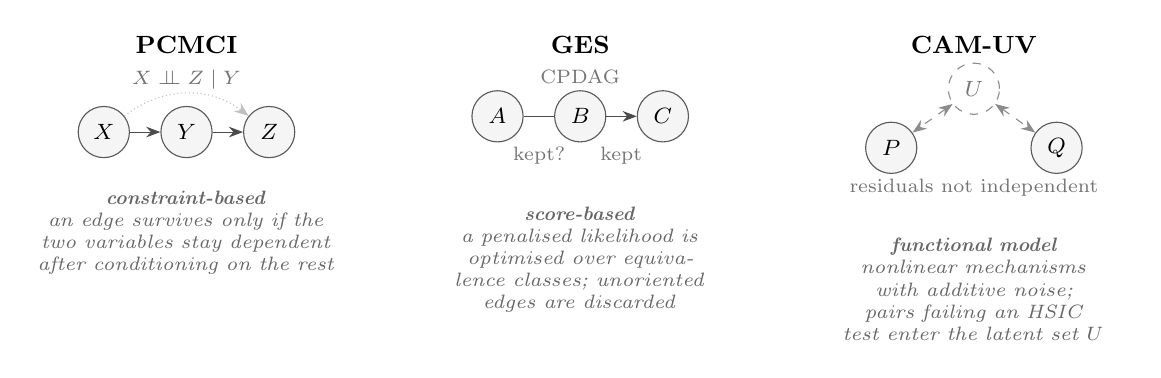
\begin{tikzpicture}[
  font=\small,
  v/.style={circle, draw=black!65, fill=black!4, minimum size=6.5mm, inner sep=0pt,
            font=\footnotesize},
  hid/.style={circle, draw=black!45, dashed, fill=none, minimum size=6.5mm,
              inner sep=0pt, font=\footnotesize, text=black!55},
  e/.style={-{Stealth[length=1.8mm]}, draw=black!70},
  und/.style={draw=black!70},
  bi/.style={{Stealth[length=1.8mm]}-{Stealth[length=1.8mm]}, draw=black!45, dashed},
  ttl/.style={font=\small\bfseries, align=center},
  sub/.style={font=\scriptsize\itshape, text=black!60, align=center, text width=38mm},
  panel/.style={draw=black!25, rounded corners=2pt, inner sep=3mm}
]

% ================================================= 1. constraint-based (PCMCI)
\begin{scope}[local bounding box=p1]
  \begin{scope}[local bounding box=d1]
    \node[ttl] (t1) at (0, 1.85) {PCMCI};
    \node[v] (x1) at (-1.05, 0.75) {$X$};
    \node[v] (y1) at ( 0.00, 0.75) {$Y$};
    \node[v] (z1) at ( 1.05, 0.75) {$Z$};
    \draw[e] (x1) -- (y1);
    \draw[e] (y1) -- (z1);
    \draw[e, bend left=38, draw=black!25, densely dotted] (x1) to (z1);
    \node[font=\scriptsize, text=black!55] at (0, 1.42) {$X \perp\!\!\!\perp Z \mid Y$};
  \end{scope}
  \node[sub, below=3mm of d1]
    {\textbf{constraint-based}\\ an edge survives only if the two variables stay
     dependent after conditioning on the rest};
\end{scope}

% ===================================================== 2. score-based (GES)
\begin{scope}[shift={(5.0, 0)}, local bounding box=p2]
  \begin{scope}[local bounding box=d2]
    \node[ttl] (t2) at (0, 1.85) {GES};
    \node[v] (a2) at (-1.05, 0.95) {$A$};
    \node[v] (b2) at ( 0.00, 0.95) {$B$};
    \node[v] (c2) at ( 1.05, 0.95) {$C$};
    \draw[und] (a2) -- (b2);
    \draw[e]   (b2) -- (c2);
    \node[font=\scriptsize, text=black!55] at (0, 1.45) {CPDAG};
    \node[font=\scriptsize, text=black!55] at (-0.52, 0.45) {kept?};
    \node[font=\scriptsize, text=black!55] at ( 0.52, 0.45) {kept};
  \end{scope}
  \node[sub, below=3mm of d2]
    {\textbf{score-based}\\ a penalised likelihood is optimised over equivalence
     classes; unoriented edges are discarded};
\end{scope}

% ============================================ 3. functional causal model (CAM-UV)
\begin{scope}[shift={(10.0, 0)}, local bounding box=p3]
  \begin{scope}[local bounding box=d3]
    \node[ttl] (t3) at (0, 1.85) {CAM-UV};
    \node[hid] (u3) at ( 0.00, 1.30) {$U$};
    \node[v]   (p3n) at (-1.05, 0.55) {$P$};
    \node[v]   (q3n) at ( 1.05, 0.55) {$Q$};
    \draw[bi] (u3) -- (p3n);
    \draw[bi] (u3) -- (q3n);
    \node[font=\scriptsize, text=black!55] at (0, 0.05) {residuals not independent};
  \end{scope}
  \node[sub, below=3mm of d3]
    {\textbf{functional model}\\ nonlinear mechanisms with additive noise; pairs failing
     an HSIC test enter the latent set $U$};
\end{scope}

\end{tikzpicture}
}
%        \caption{...}
%        \label{fig:paradigms}
%      \end{figure}
%
%  main.tex already loads tikz with arrows.meta, positioning, fit,
%  backgrounds and calc, which is everything this figure uses.
%
%  The point the figure has to make: the three algorithms are not three
%  implementations of one idea. Each rests on a different assumption about
%  what makes structure recoverable from observation alone -- conditional
%  independence, a penalised score over equivalence classes, and the
%  functional form of the mechanism. That is why a result holding across
%  all three says something about causal discovery rather than about one
%  estimator, and it is the argument of Section 2.4.
%
%  LAYOUT NOTE, because this figure has been wrong twice.
%
%  The caption block under each panel was first placed at a fixed
%  coordinate. Centred on it, a three-line block grew upward into the
%  diagram and printed on top of it: "residuals not independent" and
%  "functional model" came out overlaid as "resfunctionalmodelent" in the
%  compiled PDF. Anchoring the block at its top edge helped but still
%  relied on my guessing how tall the rows above it would render, which is
%  not something to guess at without a compiler to check against.
%
%  Each panel's diagram now sits in its own inner scope with a local
%  bounding box, and the caption is placed below that box with
%  positioning's `below=of`. TikZ then computes the clearance from what
%  actually rendered rather than from an estimate, so no combination of
%  font, text width or line count can make the two collide.
%=======================================================================
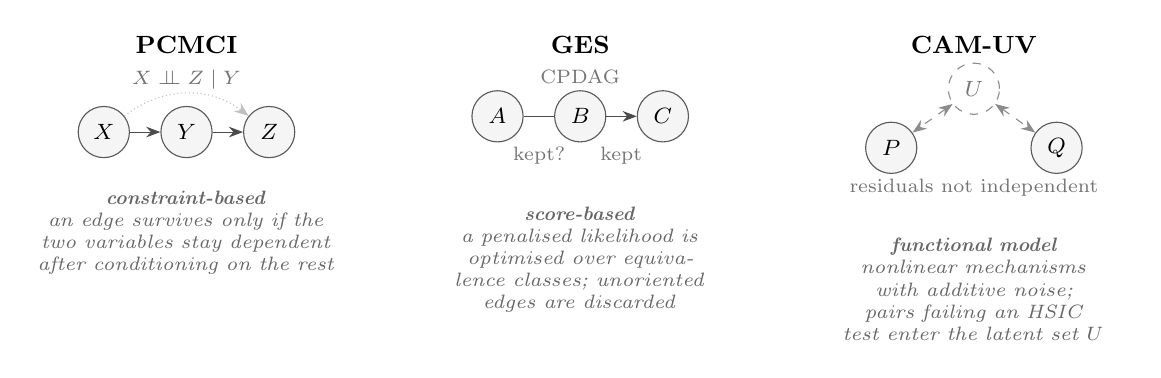
\begin{tikzpicture}[
  font=\small,
  v/.style={circle, draw=black!65, fill=black!4, minimum size=6.5mm, inner sep=0pt,
            font=\footnotesize},
  hid/.style={circle, draw=black!45, dashed, fill=none, minimum size=6.5mm,
              inner sep=0pt, font=\footnotesize, text=black!55},
  e/.style={-{Stealth[length=1.8mm]}, draw=black!70},
  und/.style={draw=black!70},
  bi/.style={{Stealth[length=1.8mm]}-{Stealth[length=1.8mm]}, draw=black!45, dashed},
  ttl/.style={font=\small\bfseries, align=center},
  sub/.style={font=\scriptsize\itshape, text=black!60, align=center, text width=38mm},
  panel/.style={draw=black!25, rounded corners=2pt, inner sep=3mm}
]

% ================================================= 1. constraint-based (PCMCI)
\begin{scope}[local bounding box=p1]
  \begin{scope}[local bounding box=d1]
    \node[ttl] (t1) at (0, 1.85) {PCMCI};
    \node[v] (x1) at (-1.05, 0.75) {$X$};
    \node[v] (y1) at ( 0.00, 0.75) {$Y$};
    \node[v] (z1) at ( 1.05, 0.75) {$Z$};
    \draw[e] (x1) -- (y1);
    \draw[e] (y1) -- (z1);
    \draw[e, bend left=38, draw=black!25, densely dotted] (x1) to (z1);
    \node[font=\scriptsize, text=black!55] at (0, 1.42) {$X \perp\!\!\!\perp Z \mid Y$};
  \end{scope}
  \node[sub, below=3mm of d1]
    {\textbf{constraint-based}\\ an edge survives only if the two variables stay
     dependent after conditioning on the rest};
\end{scope}

% ===================================================== 2. score-based (GES)
\begin{scope}[shift={(5.0, 0)}, local bounding box=p2]
  \begin{scope}[local bounding box=d2]
    \node[ttl] (t2) at (0, 1.85) {GES};
    \node[v] (a2) at (-1.05, 0.95) {$A$};
    \node[v] (b2) at ( 0.00, 0.95) {$B$};
    \node[v] (c2) at ( 1.05, 0.95) {$C$};
    \draw[und] (a2) -- (b2);
    \draw[e]   (b2) -- (c2);
    \node[font=\scriptsize, text=black!55] at (0, 1.45) {CPDAG};
    \node[font=\scriptsize, text=black!55] at (-0.52, 0.45) {kept?};
    \node[font=\scriptsize, text=black!55] at ( 0.52, 0.45) {kept};
  \end{scope}
  \node[sub, below=3mm of d2]
    {\textbf{score-based}\\ a penalised likelihood is optimised over equivalence
     classes; unoriented edges are discarded};
\end{scope}

% ============================================ 3. functional causal model (CAM-UV)
\begin{scope}[shift={(10.0, 0)}, local bounding box=p3]
  \begin{scope}[local bounding box=d3]
    \node[ttl] (t3) at (0, 1.85) {CAM-UV};
    \node[hid] (u3) at ( 0.00, 1.30) {$U$};
    \node[v]   (p3n) at (-1.05, 0.55) {$P$};
    \node[v]   (q3n) at ( 1.05, 0.55) {$Q$};
    \draw[bi] (u3) -- (p3n);
    \draw[bi] (u3) -- (q3n);
    \node[font=\scriptsize, text=black!55] at (0, 0.05) {residuals not independent};
  \end{scope}
  \node[sub, below=3mm of d3]
    {\textbf{functional model}\\ nonlinear mechanisms with additive noise; pairs failing
     an HSIC test enter the latent set $U$};
\end{scope}

\end{tikzpicture}
}
  \caption[What each discovery family uses to identify structure]{What each discovery family uses to identify structure. The three rest on incompatible assumptions about what makes a causal relation recoverable from observation alone: conditional independence after conditioning on the remaining variables, a penalised likelihood scored over Markov equivalence classes, and the functional form of the mechanism together with an independence test on the residuals.}
  \label{fig:paradigms}
\end{figure}

Two properties are claimed for discovery algorithms and they are worth defining before they are used, since both are asymptotic and both are easy to overread. An algorithm is \emph{sound} when everything it outputs is true of the generating graph: an edge it draws is a real adjacency, an arrowhead it places is a real direction. It is \emph{complete} when it outputs everything that is decidable from the information it is given, so that anything it leaves undetermined is genuinely undetermined and not merely missed. Soundness without completeness describes a cautious method that reports less than it could. Completeness without soundness describes a method that commits to answers it cannot support. Both properties are stated in the limit of infinite data and a perfect conditional independence test or a perfectly consistent score, and neither transfers to a finite sample. What they license is a reading of the algorithm's design, and what the finite sample delivers is an estimate whose errors are of the kind the design permits.

\subsection{Constraint-based discovery: PCMCI}
\label{sec:bg-pcmci}

PCMCI isolates causal links by testing conditional independence \cite{runge2019pcmci}. The test used throughout this thesis is linear partial correlation, and a property of partial correlation matters for a sensor pipeline: it is invariant to affine transformation. Discovery is therefore agnostic to the units, the scaling and the baseline offsets of the physical channels, and depends only on their conditional covariance structure.

\paragraph{Mechanism.} The procedure runs in two stages, and the reason for the second is the problem the first leaves behind. The first stage, PC$_1$, is a condition-selection pass: for each target variable it starts from the full set of lagged candidates and iteratively removes those that become conditionally independent of the target given the candidates already retained, which leaves a reduced parent set for each variable. Running this per target is what keeps the method tractable, since the alternative is a test over every subset of the remaining variables.

Condition selection alone would produce many false positives, because a test repeated across thousands of candidate links will reject the null by chance whatever the significance level. The second stage, the momentary conditional independence test, addresses this by conditioning each candidate link on the parents of both of its endpoints. Conditioning on the parents of the source as well as those of the target removes the autocorrelation in the driving variable, which is the dominant source of spurious links in time series and the reason a naive lagged correlation analysis reports structure where none exists.

\paragraph{Assumptions.} PCMCI inherits the full constraint-based list: the causal Markov condition, faithfulness, causal sufficiency and causal stationarity over the searched window, together with a conditional independence test that is valid for the data at hand. The last is not a formality. With a partial correlation test the procedure is testing linear conditional independence, so a purely nonlinear dependence with zero partial correlation is invisible to it, and the guarantee below is a guarantee about a linear world. One further assumption is specific to the lag structure. The consistency argument for PCMCI is stated for time-lagged links under the premise that contemporaneous causation is absent; where the search is extended to $\tau = 0$, the links returned at that lag are adjacencies whose orientation the procedure does not establish, and orienting them requires the additional machinery of PCMCI+ \cite{runge2020pcmciplus}.

\paragraph{Soundness and completeness.} In the oracle limit, with a consistent independence test and the assumptions above holding, the constraint-based family is sound and complete for the Markov equivalence class \cite{spirtes2000causation}: the adjacencies recovered are exactly the true ones, and the orientations are exactly those that the independencies determine. In the lagged setting completeness is stronger than in the static one, because temporal order settles every direction the independencies leave open. The momentary conditional independence stage is not part of that guarantee; it is a false-discovery control layer on top of it, and it trades power for precision. The practical consequence is a method conservative in a specific direction: it is more likely to miss a real edge than to invent one.

\paragraph{Advantages.} The test operates per target and per lag, so the search scales to wide systems where an exhaustive score comparison does not. Lags are handled natively, which means the output is already a temporal object and needs no external convention to become one. The conditional independence test is modular, so a nonlinear test can be substituted where the linear one is inadequate, and the affine invariance of partial correlation removes any need to calibrate across sensors of different physical units.

\paragraph{Drawbacks.} The number of tests grows with the number of variables and with $\tau_{\max}$, and every additional test is another opportunity to reject the null by accident, which is why an uncorrected run over a wide system tends to over-link. With a linear test the method is blind to nonlinear dependence. Causal sufficiency is assumed and never checked, so a latent common driver is returned as a direct edge with no flag on it. And the false-discovery correction that would hold the error rate at its nominal level is optional, so a configuration that omits it operates at a higher effective rate than its significance threshold suggests.

\subsection{Score-based discovery: GES}
\label{sec:bg-ges}

Greedy Equivalence Search searches the space of Markov equivalence classes directly, inserting and deleting edges to optimise a penalised likelihood \cite{chickering2002ges}. It scores whole structures rather than individual relations, which is a different epistemology from testing links one at a time.

\paragraph{Mechanism.} The search proceeds in two phases. A forward phase inserts the single edge that most improves the score, repeating until no insertion improves it. A backward phase then deletes edges on the same criterion until no deletion improves it. The backward phase is what makes the procedure more than a greedy heuristic: forward search alone will overshoot, adding edges that were justified only in the presence of others it had not yet considered, and the deletion pass is what removes them.

\paragraph{Assumptions.} GES requires the causal Markov condition, faithfulness and causal sufficiency, and in place of an independence test it requires a score that is \emph{locally consistent}: one that, in the large-sample limit, increases when an edge is added that removes a genuine dependence and decreases when an edge is added that does not. The Bayesian information criterion is locally consistent, and it is the score used here. It is also parametric. The usual formulation assumes a linear model with Gaussian errors, so its consistency is consistency within that family, and a nonlinear mechanism is scored by how well a linear model approximates it. The search also treats the observations as exchangeable: it has no representation of time, and an autocorrelated series violates the independent-sampling premise the likelihood is written under.

\paragraph{Soundness and completeness.} Chickering's result is asymptotic consistency: given a locally consistent score, causal sufficiency and a distribution faithful to some directed acyclic graph, the two phases together recover the true Markov equivalence class in the large-sample limit \cite{chickering2002ges}. That is soundness and completeness at the level of the equivalence class, which is the most any observational method can deliver without restricting the function class. Within the class the method is deliberately silent, and the undirected edges in its output are that silence written down. The guarantee is asymptotic; the samples available in any real study are finite; and the greedy search itself has no finite-sample optimality claim, so a run can terminate at a local optimum that the score would not have chosen given more data.

\paragraph{Advantages.} Scoring equivalence classes avoids the multiple-testing problem that dominates constraint-based search, because there is no sequence of hypothesis tests whose errors accumulate. The complexity penalty pushes towards sparse structures, and a sparse graph is the kind a downstream regression can actually use. The output is a single coherent structure rather than an edge list assembled from independent decisions, so it cannot contain the mutually inconsistent conclusions that separate tests sometimes produce.

\paragraph{Drawbacks.} The search is greedy over a combinatorial space and its cost grows sharply with the number of variables, which places a practical ceiling on the systems it can be run on. The default score carries a linear-Gaussian assumption that is rarely stated when results are reported. There is no notion of lag anywhere in the method, so a temporal interpretation of its output has to be supplied from outside it. And the undirected edges, correct as they are, leave a downstream consumer with a decision the algorithm has declined to make.

\subsection{Functional causal models: CAM-UV}
\label{sec:bg-camuv}

CAM-UV assumes a causal additive model with additive noise and recovers direction from the functional form of the mechanism rather than from the independence structure \cite{maeda2021camuv, buhlmann2014cam}. It is the only one of the three that does not assume causal sufficiency.

\paragraph{Mechanism and the identifiability argument.} The identifiability argument is worth stating because it is what distinguishes this family from the other two. If every mechanism were linear and every noise term Gaussian, the joint distribution would be symmetric in a way that makes the two directions of a causal edge indistinguishable, and no amount of data would separate them. Assuming the mechanisms are nonlinear breaks that symmetry \cite{hoyer2008anm}: when the true model generates the effect as a nonlinear function of the cause plus independent noise, fitting the same form in the reverse direction leaves residuals that are dependent on the putative cause. The direction that yields independent residuals is the correct one, and the test for that independence is what the method spends its effort on. Residual independence is assessed with the Hilbert-Schmidt independence criterion~\cite{gretton2005hsic}, a kernel statistic that detects dependence of any form and not only linear correlation.

Uniquely among the three, CAM-UV also reports pairs of variables it attributes to an unobserved common cause, returned as a set $U$ alongside the observed parent set $P$. The same residual machinery supports this: a pair whose dependence survives conditioning on the measured variables, and which admits no additive-noise model in either direction, is evidence of a driver that was never measured.

\paragraph{Assumptions.} The mechanisms must be additive in the noise and nonlinear in the parents, the noise must be continuous and independent across variables, and the assumed model class must contain the true mechanism. Causal sufficiency is relaxed rather than assumed, which is the method's distinctive claim. Faithfulness in the constraint-based sense is not required, since orientation comes from the residuals; what replaces it is a requirement that the independence test have power against the dependences that actually arise. Like GES, the method has no representation of time.

\paragraph{Soundness and completeness.} Within its model class the guarantee is stronger than anything the other two can offer, because the additive-noise restriction identifies the graph itself and not merely its equivalence class: the direction of a pair is decidable where the independence structure alone leaves it open. That strength is conditional in a way the other guarantees are not. Soundness holds when the true mechanism lies in the assumed class and fails without warning when it does not, because the residual independence test is then being asked to choose between two wrong models, and the direction it prefers carries no guarantee. Completeness is qualified in the other direction: pairs for which no orientation passes the test are left undecided and pairs attributed to a latent cause are reported as such, so the output is a partial description by design and not by exhaustion.

\paragraph{Advantages.} Direction is recovered beyond the Markov equivalence class, which is the single largest gain available to a method that has only observational data. Latent common causes are detected and labelled rather than quietly absorbed into a spurious edge, which is the failure mode of both other families. The kernel independence test makes no parametric commitment about the shape of the dependence it is looking for.

\paragraph{Drawbacks.} Everything rests on the model class being right, and the method does not report when it is not. Kernel independence testing is expensive in the number of observations and needs a substantial sample before it has power, which makes the method the most sample-hungry of the three. The output is not a single connected structure but a mixture of oriented pairs, undecided pairs and latent-cause pairs, and a downstream consumer has to be told what to do with each. There is no lag, as with GES. And a latent-cause pair, correct as a finding, is precisely the thing a regression on measured variables cannot represent.

\subsection{The three families side by side}
\label{sec:bg-comparison}

Table~\ref{tab:algo-comparison} sets the three against one another on the properties that matter downstream. The point of the comparison is not to rank them. It is that they fail differently, and a failure mode is what determines whether an algorithm suits a given system.

\begin{table}[htbp]
\centering
\small
\caption[The three discovery families compared]{The three discovery families compared on the properties that determine what a downstream regression receives. The guarantees in the fifth row are asymptotic in every case and none of them transfers to a finite sample.}
\label{tab:algo-comparison}
\begin{tabularx}{\textwidth}{@{}l X X X@{}}
\toprule
 & \textbf{PCMCI} & \textbf{GES} & \textbf{CAM-UV} \\
\midrule
Paradigm
  & constraint-based
  & score-based
  & functional \\[0.4em]
Evidence used
  & conditional independence of lagged and contemporaneous candidates
  & penalised likelihood over equivalence classes
  & independence of regression residuals \\[0.4em]
Key assumptions
  & Markov, faithfulness, causal sufficiency, stationarity, valid independence test
  & Markov, faithfulness, causal sufficiency, locally consistent score
  & additive nonlinear mechanisms, independent continuous noise, correct model class \\[0.4em]
Causal sufficiency
  & assumed
  & assumed
  & not assumed; latent pairs reported \\[0.4em]
Asymptotic guarantee
  & sound and complete for the equivalence class; lags oriented by time order
  & consistent for the equivalence class
  & identifies direction within the model class, beyond the equivalence class \\[0.4em]
Output object
  & a lagged graph, directed at $\tau \ge 1$
  & a completed partially directed acyclic graph, no lag
  & oriented pairs, undecided pairs and latent-cause pairs, no lag \\[0.4em]
Chief cost
  & multiple testing over many candidate links
  & combinatorial search; linear-Gaussian default score
  & kernel independence tests; sample-hungry \\[0.4em]
Fails by
  & over-linking, and silence about latent causes
  & leaving edges unoriented, and misreading nonlinearity as absence
  & committing to a direction when the model class is wrong \\
\bottomrule
\end{tabularx}
\end{table}

Three points follow from the table and they bear on everything after it.

The first concerns the type of thing each method produces, not how good it is at producing it. PCMCI emits a temporal object: an edge carries a lag and, above zero, an orientation the clock supplies for free. GES and CAM-UV emit atemporal objects, and an edge from either is a claim that two variables are related without a claim about when. Anything downstream that needs a lag has to supply one, and supplying one is an assumption of the pipeline rather than a finding of the algorithm. That distinction is carried through Chapter~\ref{ch:methodology}.

The second concerns latent causes. Two of the three assume them away. Only CAM-UV can say that a dependence it found is attributable to something nobody measured, and it says so in a form that a regression on measured variables cannot consume directly. A pipeline that takes CAM-UV seriously has to decide what to do with that set, and the decision is not neutral.

The third concerns the relationship between assumption strength and output strength, which runs the way one would expect. CAM-UV assumes the most about the mechanism and returns the most: full orientation, latent detection. GES assumes the least about functional form among the two static methods and returns the least: an equivalence class with edges it declines to orient. PCMCI sits between them and is rescued by time, since the temporal order does for its lagged edges what a functional assumption does for CAM-UV's. Each of these trades is a bet on what the system is like. None of them can be verified from the data the bet is made on, which is why an evaluation across all three says something an evaluation of any one of them cannot.

%=======================================================================
%  CHAPTER 4 -- METHODOLOGY
%=======================================================================
\chapter{Methodology}
\label{ch:methodology}

%-----------------------------------------------------------------------
\section{Overview of the Unified Pipeline}
\label{sec:method-overview}

\subsection{The five blocks}

The detector is built once and reused. Data recorded under fault-free operation enters at the left of Figure~\ref{fig:architecture} and passes through five blocks, each of which takes a definite object from the one before it and hands a definite object to the one after.

Preprocessing puts the raw channels on a common footing. It splits the record chronologically, decides which variables and which samples are carried forward, and emits a rectangular matrix of observations by variables. Causal discovery reads that matrix and returns a graph whose edges are candidate mechanisms. What the next block needs from it is narrower than a graph: for every variable, the set of other variables it will be predicted from, each with a lag attached. Turning the first object into the second is a job the pipeline does and the algorithms do not, and it is where most of this chapter's detail sits.

The baseline fit turns each parent set into a model. For every target it fits a regression of that variable on its parents, using fault-free data alone, so what the fitted coefficients encode is the plant in good health. Those coefficients are the reference the rest of the pipeline is measured against.

Online scoring is where detection happens. The same regressions are updated with a recursive least squares filter as new samples arrive, and the quantity monitored is the movement of the coefficients rather than the size of the prediction error. A relationship that still holds produces stable coefficients under the update. A relationship that has broken forces them to move. Reducing that movement across all targets gives one anomaly score per timestep, and a sample is flagged when the score passes a threshold set from fault-free data alone. Attribution then ranks the variables by how much each contributed, which turns a detection into an
explanation.

\begin{figure}[htbp]
  \centering
  \resizebox{\textwidth}{!}{%=======================================================================
%  FIGURE -- the unified detection pipeline
%
%  Include from a chapter with:
%      \begin{figure}[htbp]
%        \centering
%        %=======================================================================
%  FIGURE -- the unified detection pipeline
%
%  Include from a chapter with:
%      \begin{figure}[htbp]
%        \centering
%        \input{figures/architecture}
%        \caption{...}
%        \label{fig:architecture}
%      \end{figure}
%
%  main.tex must load TikZ. Add to the preamble:
%      \usepackage{tikz}
%      \usetikzlibrary{arrows.meta, positioning, fit, backgrounds}
%
%  The design point the figure has to make, and the reason it is worth a
%  page: three of the five stages are IDENTICAL code across all 27
%  configurations, and only two vary. Shading carries that distinction, so
%  a reader sees the experimental design before reading a word of Chapter 4.
%=======================================================================
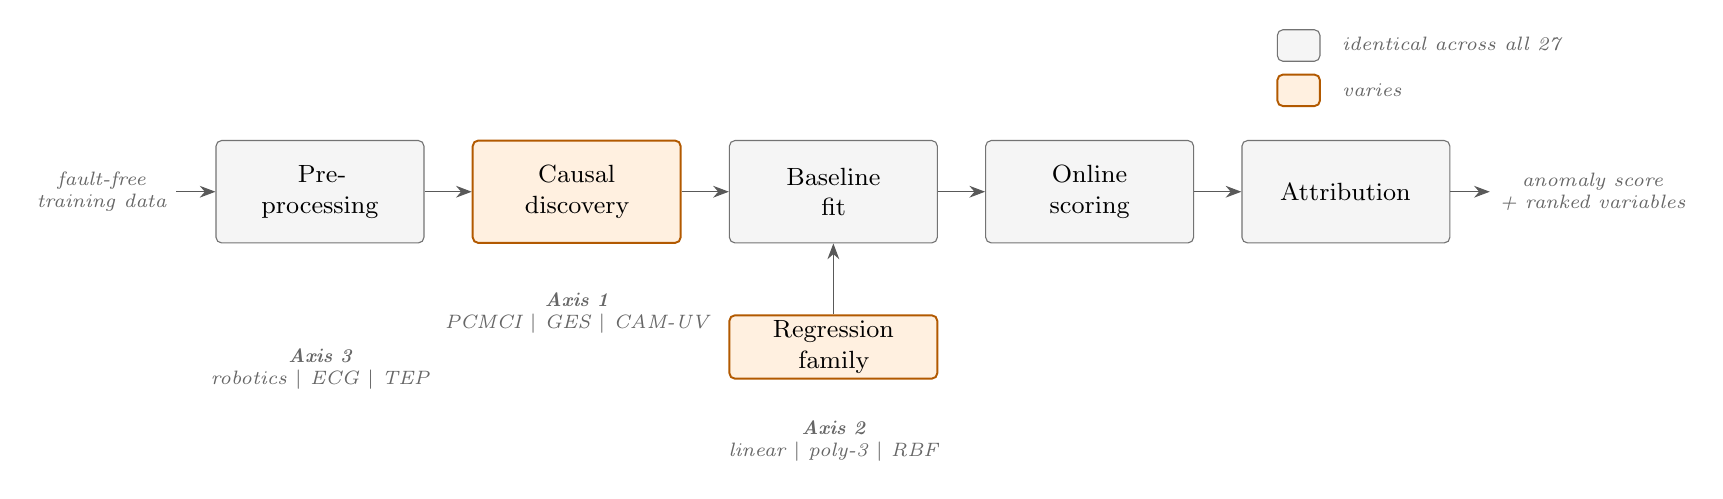
\begin{tikzpicture}[
  font=\small,
  node distance=6mm,
  fixed/.style={
    draw=black!55, fill=black!4, rounded corners=2pt,
    minimum height=13mm, text width=25mm, align=center, inner sep=2pt
  },
  varies/.style={
    draw=orange!70!black, line width=0.7pt, fill=orange!12, rounded corners=2pt,
    minimum height=13mm, text width=25mm, align=center, inner sep=2pt
  },
  lbl/.style={font=\scriptsize\itshape, text=black!60, align=center},
  ax/.style={-{Stealth[length=2mm]}, draw=black!65}
]

% ---- the five pipeline stages, left to right
\node[fixed]  (pre)  {Pre-\\processing};
\node[varies] (disc) [right=of pre]  {Causal\\discovery};
\node[fixed]  (base) [right=of disc] {Baseline\\fit};
\node[fixed]  (score)[right=of base] {Online\\scoring};
\node[fixed]  (attr) [right=of score]{Attribution};

\foreach \a/\b in {pre/disc, disc/base, base/score, score/attr}
  \draw[ax] (\a) -- (\b);

% ---- what enters and what leaves
\node[lbl] (in)  [left=5mm of pre]  {fault-free\\training data};
\node[lbl] (out) [right=5mm of attr]{anomaly score\\+ ranked variables};
\draw[ax] (in)  -- (pre);
\draw[ax] (attr) -- (out);

% ---- the second varying axis attaches to the baseline fit
\node[varies, minimum height=8mm, text width=25mm] (reg) [below=9mm of base]
  {Regression\\family};
\draw[ax] (reg) -- (base);

% ---- the three axes, annotated beneath
\node[lbl] (a1) [below=5mm of disc]
  {\textbf{Axis 1}\\PCMCI $\mid$ GES $\mid$ CAM-UV};
\node[lbl] (a2) [below=4mm of reg]
  {\textbf{Axis 2}\\linear $\mid$ poly-3 $\mid$ RBF};
\node[lbl] (a3) at ($(pre.south)+(0,-16mm)$)
  {\textbf{Axis 3}\\robotics $\mid$ ECG $\mid$ TEP};

% ---- legend
\begin{scope}[shift={($(attr.north)+(-6mm,12mm)$)}]
  \node[fixed,  minimum height=4mm, text width=4mm] (lf) {};
  \node[lbl, right=1.5mm of lf, align=left] {identical across all 27};
  \node[varies, minimum height=4mm, text width=4mm] (lv) [below=1.5mm of lf] {};
  \node[lbl, right=1.5mm of lv, align=left] {varies};
\end{scope}

\end{tikzpicture}

%        \caption{...}
%        \label{fig:architecture}
%      \end{figure}
%
%  main.tex must load TikZ. Add to the preamble:
%      \usepackage{tikz}
%      \usetikzlibrary{arrows.meta, positioning, fit, backgrounds}
%
%  The design point the figure has to make, and the reason it is worth a
%  page: three of the five stages are IDENTICAL code across all 27
%  configurations, and only two vary. Shading carries that distinction, so
%  a reader sees the experimental design before reading a word of Chapter 4.
%=======================================================================
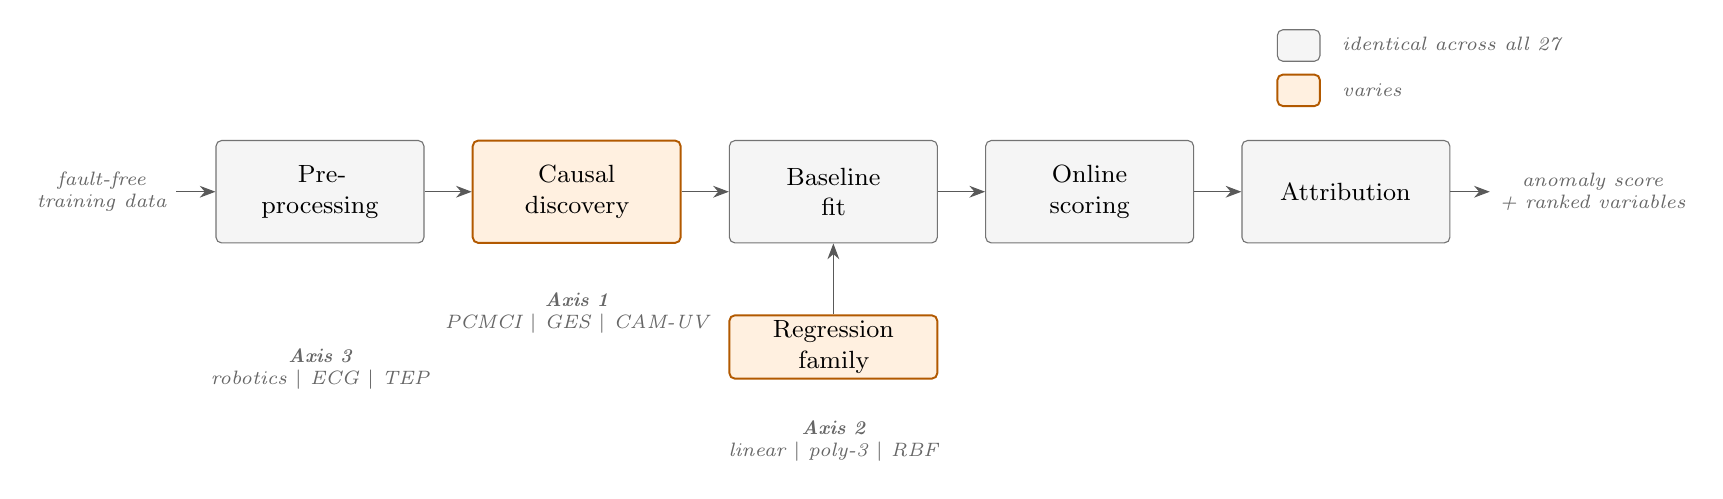
\begin{tikzpicture}[
  font=\small,
  node distance=6mm,
  fixed/.style={
    draw=black!55, fill=black!4, rounded corners=2pt,
    minimum height=13mm, text width=25mm, align=center, inner sep=2pt
  },
  varies/.style={
    draw=orange!70!black, line width=0.7pt, fill=orange!12, rounded corners=2pt,
    minimum height=13mm, text width=25mm, align=center, inner sep=2pt
  },
  lbl/.style={font=\scriptsize\itshape, text=black!60, align=center},
  ax/.style={-{Stealth[length=2mm]}, draw=black!65}
]

% ---- the five pipeline stages, left to right
\node[fixed]  (pre)  {Pre-\\processing};
\node[varies] (disc) [right=of pre]  {Causal\\discovery};
\node[fixed]  (base) [right=of disc] {Baseline\\fit};
\node[fixed]  (score)[right=of base] {Online\\scoring};
\node[fixed]  (attr) [right=of score]{Attribution};

\foreach \a/\b in {pre/disc, disc/base, base/score, score/attr}
  \draw[ax] (\a) -- (\b);

% ---- what enters and what leaves
\node[lbl] (in)  [left=5mm of pre]  {fault-free\\training data};
\node[lbl] (out) [right=5mm of attr]{anomaly score\\+ ranked variables};
\draw[ax] (in)  -- (pre);
\draw[ax] (attr) -- (out);

% ---- the second varying axis attaches to the baseline fit
\node[varies, minimum height=8mm, text width=25mm] (reg) [below=9mm of base]
  {Regression\\family};
\draw[ax] (reg) -- (base);

% ---- the three axes, annotated beneath
\node[lbl] (a1) [below=5mm of disc]
  {\textbf{Axis 1}\\PCMCI $\mid$ GES $\mid$ CAM-UV};
\node[lbl] (a2) [below=4mm of reg]
  {\textbf{Axis 2}\\linear $\mid$ poly-3 $\mid$ RBF};
\node[lbl] (a3) at ($(pre.south)+(0,-16mm)$)
  {\textbf{Axis 3}\\robotics $\mid$ ECG $\mid$ TEP};

% ---- legend
\begin{scope}[shift={($(attr.north)+(-6mm,12mm)$)}]
  \node[fixed,  minimum height=4mm, text width=4mm] (lf) {};
  \node[lbl, right=1.5mm of lf, align=left] {identical across all 27};
  \node[varies, minimum height=4mm, text width=4mm] (lv) [below=1.5mm of lf] {};
  \node[lbl, right=1.5mm of lv, align=left] {varies};
\end{scope}

\end{tikzpicture}
}
  \caption[The unified detection pipeline]{The unified detection pipeline. Preprocessing, baseline fit, online scoring and attribution are identical in every configuration; only the causal discovery step and the regression family vary, and those are the two methodological axes this chapter declares. The third annotation in the diagram marks the data entering at the left, which changes no stage of the pipeline and belongs to the experimental design of Chapter~\ref{ch:experimental_setup} rather than to the method.}
  \label{fig:architecture}
\end{figure}

Each block gets its own section below. The order of the sections is the order of the arrows, and each one states four things: what enters, what leaves, what has to be true for the block to be doing what it claims, and why the next block cannot proceed without what this one produces. The algorithms themselves are not re-described here; they belong to Chapter~\ref{ch:background}, and what matters at this level is the shape of what they emit.

\subsection{What varies and what is held fixed}

The methodology has two axes. The first is the causal discovery algorithm, which decides what each regression is allowed to look at. The second is the regression family, which decides what functional form the fit may take. Crossing three algorithms with three regression variants gives nine methodological combinations, and the same nine are instantiated on each of the three application domains described in Chapter~\ref{ch:experimental_setup}, which is how the study arrives at 27 configurations in total. The domain is not a third axis of the method. It changes the data entering at the left and nothing downstream of it.

The diagram carries the experimental design as well as the data flow. Of the five blocks, three are identical in every configuration and only two vary. Shading marks that distinction, so a reader can see what is controlled before reading the argument for it.

Comparability comes from holding the downstream detector constant while varying its inputs. Preprocessing is deliberately not uniform. As set out in Section~\ref{sec:method-preprocessing}, the subsampling rate and the variable inclusion cap are treated as intrinsic properties of each algorithm's operational workflow instead of as free parameters to be equalised. Research Question~1 therefore compares each algorithm as it is intended to be applied, preprocessing included, and does not isolate the discovery step. The cost of that decision is quantified in Chapter~\ref{ch:results}.

What remains strictly uniform is the whole of the downstream detection machinery: the recursive least squares update, the coefficient drift score, the thresholding rule and the attribution depth. That is a programmatically enforced claim and not an aspirational one, verified by a suite of seventeen automated checks on every build. The most consequential of them audits every configuration for any step that would fit a decision threshold to the evaluation labels, and fails the build if one is found, so no configuration can quietly improve its reported figures by selecting its own operating point against the answers.

%-----------------------------------------------------------------------
\section{Block One: Preprocessing}
\label{sec:method-preprocessing}

\paragraph{Input and output.} The block receives the raw multivariate record as it comes off the instrument, with its native sampling rate, its native units and its full channel list. It emits two matrices of observations by variables: a fault-free training partition on which discovery and the baseline fit are performed, and an evaluation partition that is never seen until the online pass. Nothing downstream ever touches the raw record.

\paragraph{The chronological split.} The first operation divides the record in time, taking the earlier portion as the fault-free training baseline and holding out the remainder for evaluation. The proportion is fixed at 70\% and 30\% in every configuration. A chronological division is a necessity rather than a convention. A randomised split over a time series places future observations in the training set, and because consecutive samples are strongly dependent this leaks information in a way a random split over independent observations does not. The leak is not visible in the resulting scores, which is why it is dangerous. The proportion is not free of consequences elsewhere. On the plant it leaves discovery 35 samples for 52 variables at the protocol's subsampling rate, which is 0.67 observations per variable, and Chapter~\ref{ch:experimental_setup} shows the recovered graph densifying monotonically as that count grows. The sparsity of the industrial graphs is a property of this split before it is a property of the process.

\paragraph{Variable selection and subsampling.} The second operation decides how wide and how long the matrix is. Both quantities are treated as properties of each algorithm's workflow rather than as uniform pipeline constraints, because neither is free in both directions: a score-based search over a wide system fails to converge at variable counts a constraint-based search handles without difficulty, and equalising downwards would mean evaluating one algorithm on a problem nobody would give it. The inclusion cap and the sample retention rate therefore vary by algorithm, and the values applied in each case are tabulated in Chapter~\ref{ch:experimental_setup} and Appendix~\ref{app:hyperparameters}. This is the study's principal threat to internal validity. It is declared here, not conceded later, and it is quantified rather than left as a word. PCMCI selects its retention rate per domain, taking 74 on Robotics, 7 on Healthcare and 1 on Industrial, where GES and CAM-UV are fixed at 10 throughout and capped at 35 variables besides. Two ablations bound what that costs. Forcing PCMCI to rate 10 on Robotics drops it from 0.8752 to 0.6813; forcing GES to rate 1 on Healthcare drops it from 0.8114 to 0.6184. The rate is therefore not a nuisance parameter, and the comparison RQ1 asks for is foreclosed by it: 54 of the 108 within-domain comparisons admit no paired test, every one of them involving PCMCI against another algorithm.

\paragraph{Standardisation, and where it actually happens.} The third operation is $z$-score standardisation, applied per target rather than globally. A separate scaler is fitted over the causal parents of each individual target variable, using the training partition alone, and the fitted scalers are retained so that the online pass applies the identical transform. Strictly, this straddles two blocks: a scaler defined over a target's parents cannot be fitted until the parent sets exist, so the operation is specified here and executed once the graph has been normalised. One consequence affects how coefficients are read. The same physical sensor may receive a different scaling depending on which target's regression it appears in, so coefficient magnitudes are comparable within a target and not across targets.

\paragraph{Assumptions.} The block assumes the training partition is fault-free, which is an assumption about the data and not something the pipeline can verify. It assumes the record is stationary enough over the training window for a scaler fitted there to remain valid on the evaluation window. And by subsampling it assumes that the dynamics of interest survive at the reduced rate, which is a bet on the bandwidth of the process relative to the retention rate chosen.

\paragraph{Why the next block needs this.} Causal discovery operates on a matrix whose rows are observations and whose columns are variables, and every one of the three algorithms will accept a transposed matrix without complaint and return a plausible graph over the wrong objects. Fixing the orientation, the width and the length here means the discovery block has one well-defined input and no opportunity to silently reinterpret it.

%-----------------------------------------------------------------------
\section{Block Two: Causal Discovery}
\label{sec:method-axis1}

\paragraph{Input and output.} The block receives the fault-free training matrix and returns a graph. What it does internally is one of the three procedures of Chapter~\ref{ch:background} and is not restated here. What matters at this level is that the three return objects of different types, and the pipeline needs one type.

PCMCI returns a lagged graph: an edge carries the identity of the parent, the identity of the child and the lag between them. GES returns a completed partially directed acyclic graph over the unlagged matrix, in which some edges are oriented and some are not, and none carries a lag. CAM-UV returns two sets over the unlagged matrix, the observed parent set $P$ and the set $U$ of variable pairs it attributes to an unobserved common cause, and neither carries a lag either. A regression cannot be fitted to any of those three directly.

\begin{figure}[htbp]
  \centering
  \resizebox{\textwidth}{!}{%
  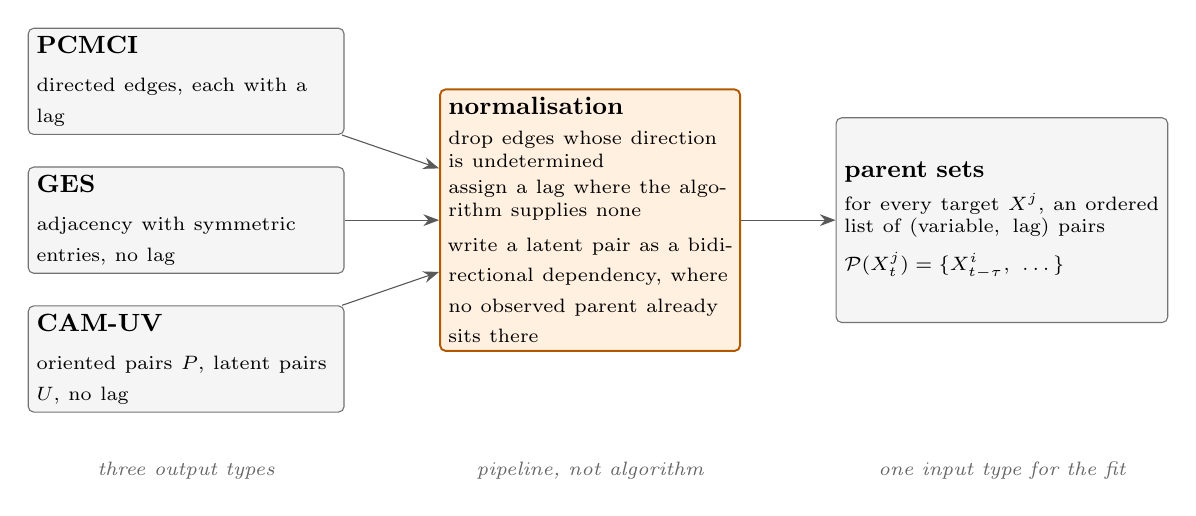
\begin{tikzpicture}[
    font=\small,
    emit/.style={draw=black!55, fill=black!4, rounded corners=2pt,
                 text width=38mm, align=left, inner sep=3pt, minimum height=13mm},
    proc/.style={draw=orange!70!black, line width=0.7pt, fill=orange!12,
                 rounded corners=2pt, text width=36mm, align=left, inner sep=3pt,
                 minimum height=26mm},
    pset/.style={draw=black!55, fill=black!4, rounded corners=2pt,
                 text width=40mm, align=left, inner sep=3pt, minimum height=26mm},
    cpt/.style={font=\scriptsize\itshape, text=black!60, align=center},
    ar/.style={-{Stealth[length=2mm]}, draw=black!65}
  ]
    \node[emit] (e1) {\textbf{PCMCI}\\[1mm]\scriptsize directed edges, each with a lag};
    \node[emit] (e2) [below=4mm of e1] {\textbf{GES}\\[1mm]\scriptsize adjacency with symmetric entries, no lag};
    \node[emit] (e3) [below=4mm of e2] {\textbf{CAM-UV}\\[1mm]\scriptsize oriented pairs $P$, latent pairs $U$, no lag};

    \node[proc] (norm) [right=12mm of e2]
      {\textbf{normalisation}\\[1mm]\scriptsize
       drop edges whose direction is undetermined\\[0.6mm]
       assign a lag where the algorithm supplies none\\[0.6mm]
       write a latent pair as a bidirectional dependency, where no observed parent already sits there};

    \node[pset] (ps) [right=12mm of norm]
      {\textbf{parent sets}\\[1mm]\scriptsize
       for every target $X^j$, an ordered list of $(\text{variable},\ \text{lag})$ pairs\\[1mm]
       $\mathcal{P}(X^j_t) = \{X^{i}_{t-\tau},\ \dots\}$};

    \foreach \a in {e1,e2,e3} \draw[ar] (\a) -- (norm);
    \draw[ar] (norm) -- (ps);

    \node[cpt] (c1) [below=5mm of e3] {three output types};
    \node[cpt] (c2) at (norm |- c1) {pipeline, not algorithm};
    \node[cpt] (c3) at (ps |- c1) {one input type for the fit};
  \end{tikzpicture}}
  \caption[What the discovery block emits and what the fit receives]{What the discovery block emits and what the baseline fit receives. The three algorithms return objects of three different types, and only the rightmost one can be regressed on. The middle box is the pipeline's work and not the algorithms': every edge that reaches a regression as a lagged parent of a particular target does so under a rule stated in this section, which means the lag structure of a GES or CAM-UV graph is a property of this pipeline and not a finding of the discovery step.}
  \label{fig:graph-normalisation}
\end{figure}

\subsection{From a discovered graph to a parent set}
\label{sec:integration-verification}

The conversion is shown in Figure~\ref{fig:graph-normalisation}. Four rules do the work, and each of them is a decision the pipeline makes on the algorithm's behalf.

\paragraph{Undetermined directions are dropped.} An edge is retained only where the adjacency entries agree that the direction is determined, which is to say only where the graph asserts an unambiguous $i \to j$ relation. Where the search declined to orient an edge, the pipeline declines too. The alternative would be to orient by convention, which would hand the regressor a parent the data does not support, and the undirected edge exists precisely because the data cannot choose. Some information is lost this way. That is the correct price. What it buys, and what it costs, can both be counted. A variable reached only by edges the search declined to orient receives no parent at all and drops out of the detector entirely, which is why GES enters the regression stage with nine targets of the twelve electrocardiogram leads and twenty-five of the plant's fifty-two variables. Those are mechanisms the detector cannot watch. The alternative was to invent directions for them.

\paragraph{A missing lag is assigned, not discovered.} An algorithm run on the unlagged matrix returns an edge that says two variables are related and says nothing about when. Before it can enter a regression that differences an offline baseline against an online pass, a lag has to be attached. The pipeline attaches one, uniformly within a configuration, and the value used in each case is recorded in Chapter~\ref{ch:experimental_setup}. This point is laboured because it is easy to misread a figure of a GES or CAM-UV graph as a temporal claim. It is not one. PCMCI is the only one of the three whose lags are discovered. Where they land narrows the distinction considerably. Measured against the cached graphs under the sparsification rule and the cap below, 100.0\% of the parent slots PCMCI's regressions retain on Healthcare and on Robotics sit at lag zero, and 98.7\% do on Industrial. So the algorithm that discovers its lags almost always discovers zero, and the assigned lag the other two receive differs from the discovered one less often than this paragraph's emphasis implies.

\paragraph{Latent pairs are written as bidirectional dependencies.} CAM-UV's set $U$ names pairs whose dependence it attributes to something nobody measured. The scoring mechanism cannot regress on an unmeasured signal, so each such pair is written into the final graph as a bidirectional dependency, forcing each variable to account for the other's variance without representing the cause explicitly. Observed parents take strict precedence: a pair is written from $U$ only where no edge from $P$ already occupies that position. The rule preserves the statistical linkage the algorithm found and is honest about what it is doing, which is substituting a proxy for a cause that was never recorded. How much of a graph that substitution accounts for varies enormously by domain, and on one of the three it accounts for all of it. CAM-UV assigns 480 robot variable pairs to $U$, a saturation of 80.7\%, and returns no observed-parent edge whatsoever, so every edge the detector receives there is a proxy. On the electrocardiogram 39 of the 48 linked pairs come from $U$, and on the plant 14 of 49. Appendix~\ref{app:confounders} separates the two counts in each domain.

\paragraph{The graph is sparsified before use.} A threshold is applied to the retained edge set before parent lists are built, with the multiplier tabulated in Appendix~\ref{app:hyperparameters}. On a dense graph this is the difference between a parent list that reflects the search and one that reflects whatever survived an arbitrary truncation later. In practice the rule barely fires. Across all nine algorithm-domain configurations the effect-size filter removes edges in exactly one, PCMCI on healthcare, where it discards three of 66 variable pairs. The reason is that GES and CAM-UV supply edge indicators and not continuous strengths, so for those two the filter compares 1.0 against the mean of a sparse indicator matrix and every edge survives it. Graph density is therefore settled by what each algorithm discovers, not by this rule.

\paragraph{Assumptions.} The block assumes the training window satisfies the standing assumptions of Section~\ref{sec:bg-assumptions} for whichever algorithm is running, and those differ: two of the three assume causal sufficiency and one does not. It assumes the matrix orientation is correct, which the previous block guarantees and which no algorithm checks. And the lag-assignment rule assumes that a relation the algorithm found without reference to time is adequately represented at the single lag chosen, which is the weakest assumption in the pipeline and is not defensible in general. It is stated so that the results obtained under it can be read with that in view.

\paragraph{Why the next block needs a regression at all.} A graph is a statement about which variables are related. It is not a statement about how, and a detector cannot be built from it directly, because a graph is a fixed object and a fault is a change. What changes when a mechanism breaks is the strength and the shape of the dependence, not usually the existence of the edge. Fitting a regression to each parent set converts the qualitative claim into a quantitative one: a coefficient vector that has a value under normal operation and a different value once the mechanism has altered. The graph decides what the model may look at; the regression is what supplies a number that can move. This is the reason the pipeline does not stop at discovery, and it is also why a discovery error is costly downstream, since a missing parent leaves a mechanism unmodelled and a spurious parent gives the filter a coefficient with nothing real to track.

%-----------------------------------------------------------------------
\section{Block Three: Baseline Fit}
\label{sec:method-baseline}

\paragraph{Input and output.} The block receives the parent sets and the fault-free training partition. For every target it emits three things that the online pass will need: a fitted scaler over that target's parents, a feature map, and a baseline coefficient vector $\mathbf{w}^{(0)}_v$ including an intercept. Everything the detector later calls normal is contained in those vectors.

\subsection{The parent cap}
\label{sec:parent-cap}

A target is not regressed on every parent its graph supplies. The incoming edges are sorted by lag and the three shortest-lag parents are kept, so the design matrix is at most three columns wide plus the intercept, in every configuration and irrespective of how dense the graph is. Ties are resolved by variable index.

Figure~\ref{fig:parentcap-diagram} shows the selection concretely, because the mechanism is easy to misread as a tie-break among near-equal candidates. It is nothing of the kind. Temporal position decides what survives, and the strength of the evidence the discovery step weighed decides nothing at all. The cap is uniform as a rule and radically uneven as an intervention. On robotics it discards 98.2\% of the edges PCMCI found and none at all of what GES found; on healthcare, 75.8\% against 26.5\%. A comparison run under it therefore sets a whole graph against a small selection from another, and where the cap binds hardest the surviving parent set is settled substantially by lag order and a tiebreak on variable index rather than by the search. Chapter~\ref{ch:results} measures the bite for all nine pairs.

\begin{figure}[htbp]
  \centering
  \resizebox{0.92\textwidth}{!}{%=======================================================================
%  FIGURE -- how the three-parent cap selects a design matrix
%
%  Include from a chapter with:
%      \begin{figure}[htbp]
%        \centering
%        %=======================================================================
%  FIGURE -- how the three-parent cap selects a design matrix
%
%  Include from a chapter with:
%      \begin{figure}[htbp]
%        \centering
%        \input{figures/parent_cap}
%        \caption{...}
%        \label{fig:parentcap-diagram}
%      \end{figure}
%
%  Uses only tikz with arrows.meta, already loaded by main.tex. Every node
%  is written out rather than generated in a loop, and there is no
%  conditional or pgfmath in the body, so the figure cannot fail in a way
%  that depends on how TikZ expands a loop variable.
%
%  The point: the cap is not a tie-break among near-equal candidates. It
%  sorts the incoming edges by LAG and keeps the first three, so on a dense
%  graph the parents reaching the regression are chosen by an ordering that
%  carries no information about edge strength. The numbers are the measured
%  healthcare PCMCI case from tools/parent_cap_bite.csv: 12.42 candidate
%  parents per target on average, reduced to exactly 3.00.
%
%  The lag labels are the measured healthcare PCMCI case too, not a generic
%  illustration: tools/parent_cap_lag.py finds that on Healthcare PCMCI's
%  candidates are dominated by tau=0 (contemporaneous) edges, and that every
%  one of the three the cap actually keeps is tau=0 -- not tau=1 as an
%  earlier version of this figure showed. tau=4 is also not a value PCMCI
%  can produce on Healthcare, where tau_max=3, so the dropped candidates
%  are relabelled within range as well. See Section 3.1 and Section 4.3.
%=======================================================================
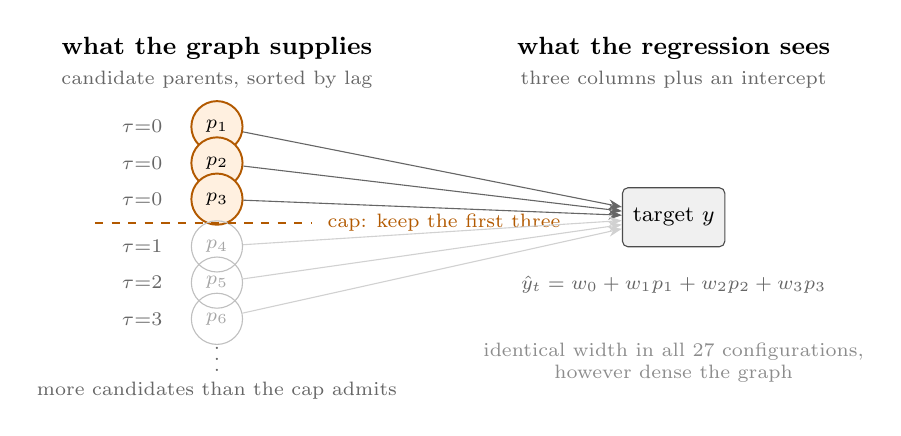
\begin{tikzpicture}[
  font=\small,
  keptn/.style={circle, draw=orange!70!black, line width=0.7pt, fill=orange!12,
                minimum size=6.5mm, inner sep=0pt, font=\scriptsize},
  dropn/.style={circle, draw=black!25, fill=none, minimum size=6.5mm, inner sep=0pt,
                font=\scriptsize, text=black!35},
  tgt/.style={rectangle, rounded corners=2pt, draw=black!70, fill=black!6,
              minimum height=7.5mm, minimum width=13mm, font=\footnotesize},
  e/.style={-{Stealth[length=1.7mm]}, draw=black!60},
  eg/.style={-{Stealth[length=1.7mm]}, draw=black!18},
  lbl/.style={font=\scriptsize, text=black!60, align=center},
  hd/.style={font=\small\bfseries, align=center}
]

% ---------------------------------------------- left: what the graph supplies
\node[hd]  at (-1.5,  2.45) {what the graph supplies};
\node[lbl] at (-1.5,  2.05) {candidate parents, sorted by lag};

\node[keptn] (c0) at (-1.5,  1.45) {$p_{1}$};
\node[keptn] (c1) at (-1.5,  0.99) {$p_{2}$};
\node[keptn] (c2) at (-1.5,  0.53) {$p_{3}$};
\node[dropn] (c3) at (-1.5, -0.07) {$p_{4}$};
\node[dropn] (c4) at (-1.5, -0.53) {$p_{5}$};
\node[dropn] (c5) at (-1.5, -0.99) {$p_{6}$};

\node[lbl] at (-2.45,  1.45) {$\tau{=}0$};
\node[lbl] at (-2.45,  0.99) {$\tau{=}0$};
\node[lbl] at (-2.45,  0.53) {$\tau{=}0$};
\node[lbl] at (-2.45, -0.07) {$\tau{=}1$};
\node[lbl] at (-2.45, -0.53) {$\tau{=}2$};
\node[lbl] at (-2.45, -0.99) {$\tau{=}3$};

\node[lbl] at (-1.5, -1.40) {$\vdots$};
\node[lbl] at (-1.5, -1.90) {more candidates than the cap admits};

% ---------------------------------------------- the cap
\draw[dashed, draw=orange!70!black, line width=0.6pt] (-3.05, 0.23) -- (-0.30, 0.23);
\node[lbl, text=orange!70!black, anchor=west] at (-0.22, 0.23) {cap: keep the first three};

% ---------------------------------------------- right: the regression
\node[tgt] (y) at (4.3, 0.30) {target $y$};

\draw[e]  (c0) -- (y);
\draw[e]  (c1) -- (y);
\draw[e]  (c2) -- (y);
\draw[eg] (c3) -- (y);
\draw[eg] (c4) -- (y);
\draw[eg] (c5) -- (y);

\node[hd]  at (4.3,  2.45) {what the regression sees};
\node[lbl] at (4.3,  2.05) {three columns plus an intercept};
\node[lbl] at (4.3, -0.55) {$\hat{y}_t = w_0 + w_1 p_1 + w_2 p_2 + w_3 p_3$};
\node[lbl, text=black!45] at (4.3, -1.55)
  {identical width in all 27 configurations,\\ however dense the graph};

\end{tikzpicture}

%        \caption{...}
%        \label{fig:parentcap-diagram}
%      \end{figure}
%
%  Uses only tikz with arrows.meta, already loaded by main.tex. Every node
%  is written out rather than generated in a loop, and there is no
%  conditional or pgfmath in the body, so the figure cannot fail in a way
%  that depends on how TikZ expands a loop variable.
%
%  The point: the cap is not a tie-break among near-equal candidates. It
%  sorts the incoming edges by LAG and keeps the first three, so on a dense
%  graph the parents reaching the regression are chosen by an ordering that
%  carries no information about edge strength. The numbers are the measured
%  healthcare PCMCI case from tools/parent_cap_bite.csv: 12.42 candidate
%  parents per target on average, reduced to exactly 3.00.
%
%  The lag labels are the measured healthcare PCMCI case too, not a generic
%  illustration: tools/parent_cap_lag.py finds that on Healthcare PCMCI's
%  candidates are dominated by tau=0 (contemporaneous) edges, and that every
%  one of the three the cap actually keeps is tau=0 -- not tau=1 as an
%  earlier version of this figure showed. tau=4 is also not a value PCMCI
%  can produce on Healthcare, where tau_max=3, so the dropped candidates
%  are relabelled within range as well. See Section 3.1 and Section 4.3.
%=======================================================================
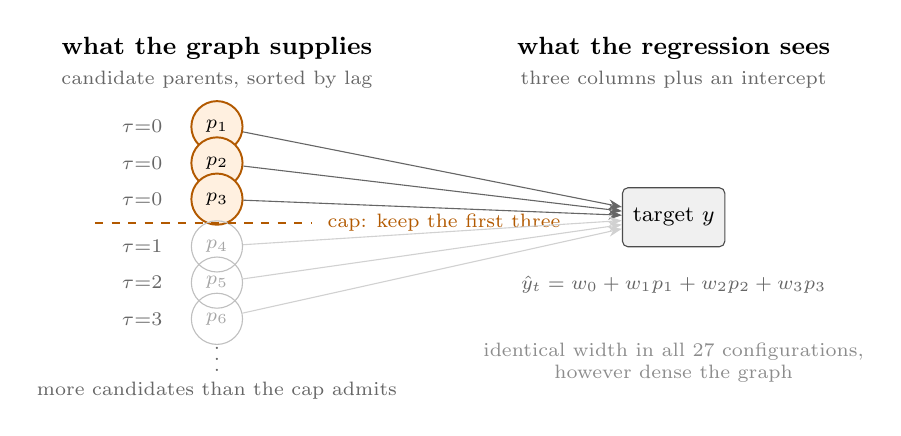
\begin{tikzpicture}[
  font=\small,
  keptn/.style={circle, draw=orange!70!black, line width=0.7pt, fill=orange!12,
                minimum size=6.5mm, inner sep=0pt, font=\scriptsize},
  dropn/.style={circle, draw=black!25, fill=none, minimum size=6.5mm, inner sep=0pt,
                font=\scriptsize, text=black!35},
  tgt/.style={rectangle, rounded corners=2pt, draw=black!70, fill=black!6,
              minimum height=7.5mm, minimum width=13mm, font=\footnotesize},
  e/.style={-{Stealth[length=1.7mm]}, draw=black!60},
  eg/.style={-{Stealth[length=1.7mm]}, draw=black!18},
  lbl/.style={font=\scriptsize, text=black!60, align=center},
  hd/.style={font=\small\bfseries, align=center}
]

% ---------------------------------------------- left: what the graph supplies
\node[hd]  at (-1.5,  2.45) {what the graph supplies};
\node[lbl] at (-1.5,  2.05) {candidate parents, sorted by lag};

\node[keptn] (c0) at (-1.5,  1.45) {$p_{1}$};
\node[keptn] (c1) at (-1.5,  0.99) {$p_{2}$};
\node[keptn] (c2) at (-1.5,  0.53) {$p_{3}$};
\node[dropn] (c3) at (-1.5, -0.07) {$p_{4}$};
\node[dropn] (c4) at (-1.5, -0.53) {$p_{5}$};
\node[dropn] (c5) at (-1.5, -0.99) {$p_{6}$};

\node[lbl] at (-2.45,  1.45) {$\tau{=}0$};
\node[lbl] at (-2.45,  0.99) {$\tau{=}0$};
\node[lbl] at (-2.45,  0.53) {$\tau{=}0$};
\node[lbl] at (-2.45, -0.07) {$\tau{=}1$};
\node[lbl] at (-2.45, -0.53) {$\tau{=}2$};
\node[lbl] at (-2.45, -0.99) {$\tau{=}3$};

\node[lbl] at (-1.5, -1.40) {$\vdots$};
\node[lbl] at (-1.5, -1.90) {more candidates than the cap admits};

% ---------------------------------------------- the cap
\draw[dashed, draw=orange!70!black, line width=0.6pt] (-3.05, 0.23) -- (-0.30, 0.23);
\node[lbl, text=orange!70!black, anchor=west] at (-0.22, 0.23) {cap: keep the first three};

% ---------------------------------------------- right: the regression
\node[tgt] (y) at (4.3, 0.30) {target $y$};

\draw[e]  (c0) -- (y);
\draw[e]  (c1) -- (y);
\draw[e]  (c2) -- (y);
\draw[eg] (c3) -- (y);
\draw[eg] (c4) -- (y);
\draw[eg] (c5) -- (y);

\node[hd]  at (4.3,  2.45) {what the regression sees};
\node[lbl] at (4.3,  2.05) {three columns plus an intercept};
\node[lbl] at (4.3, -0.55) {$\hat{y}_t = w_0 + w_1 p_1 + w_2 p_2 + w_3 p_3$};
\node[lbl, text=black!45] at (4.3, -1.55)
  {identical width in all 27 configurations,\\ however dense the graph};

\end{tikzpicture}
}
  \caption[How the three-parent cap selects a design matrix]{How the three-parent cap selects a design matrix. The incoming edges of a target are ordered by lag, closest first, and the first three are kept. The surviving parents are therefore chosen by temporal position rather than by the strength of the evidence the discovery step weighed, and on a dense graph the parent set is settled substantially by an arbitrary tiebreak. The design matrix is the same width in every configuration, however dense the graph that fed it.}
  \label{fig:parentcap-diagram}
\end{figure}

The bound is not a parameter of this study and was not selected against any result. It is retained from the reference implementation, which sorts by lag and truncates at three identically, and it is kept for the same parity reason that governs the attribution rules of Section~\ref{sec:method-attribution}. The same reference fixes the depth at which attributions are tabulated, which is why that is also three.

Two consequences pull in opposite directions and both belong in the record. The cap equalises regression capacity across the three algorithms, so a performance difference within a domain cannot be attributed to one algorithm having been handed a larger model to fit, which is what the controlled comparison of Research Question~1 requires. Against that, it does not remove the same number of edges from each algorithm, because the algorithms do not produce graphs of comparable density. Where the cap binds hard, the surviving parents are chosen by lag order with ties broken on an index, so the parent set is settled substantially by an arbitrary rule rather than by the discovery step that was supposed to determine it. A dense graph therefore does not give the regression more to work with. It gives the tiebreak more to do. How often the bound binds for each algorithm, and what follows from it, is measured in Chapter~\ref{ch:results}.

\subsection{The regression family}
\label{sec:method-regression}

The second methodological axis varies the functional form of the fit while leaving the parent set untouched. Three variants are used: linear, a polynomial expansion of degree three, and a radial basis function feature map. The point of the axis is to test whether the linearity implicit in most of the pipeline is a limitation or an adequate approximation, and it is a fair test only because the parent sets are identical across the three.

The RBF variant uses random Fourier features, a randomised low-rank approximation to the RBF kernel~\cite{rahimi2007random}, which then feeds the same linear estimator. It is a feature expansion and not a radial basis function network, and the distinction matters because the coefficients the detector monitors are coefficients on explicit features, which a kernel method would not provide.

\subsection{Feature maps and regularisation}
\label{sec:bg-features}

Expanding a parent set polynomially or through a Fourier map raises the dimension quickly and produces strongly correlated features. Left unpenalised, that collinearity leaves the design matrix ill-conditioned and the least squares solution unstable, which for a drift detector is fatal rather than merely inconvenient: an unstable solution moves for numerical reasons and the detector cannot tell that movement from a fault. All three variants therefore apply an $L_2$ ridge penalty~\cite{hoerl1970ridge}.

Standardisation is applied to the parent variables before the expansion, and the order matters. An $L_2$ penalty is isotropic in the coordinates it is given, so without prior standardisation a variable with a large native magnitude receives proportionally less shrinkage than one with a small magnitude, and the penalty stops being neutral between parents.

The regularisation strength requires a statement, because it bounds the empirical claims that follow. In two of the three domains it is held constant at 10.0 across every configuration. The third is Robotics, where it varies by regression variant, taking 10.0 for the linear map, 0.01 for the degree-three polynomial and 1.0 for the random Fourier features, because a degree-three expansion and a random-feature map over that domain's parent sets produce design matrices too poorly conditioned to fit under the stronger penalty. That was an engineering necessity and not a tuning choice, and the values are tabulated in Appendix~\ref{app:hyperparameters}. The structural invariant is that the penalty varies by domain and feature map but is identical across all three algorithms within every cell, which an automated check enforces on every build.

Reporting this here rather than in a limitations list makes clear which comparisons are strictly controlled and which are partially confounded. For Research Question~1, comparing the discovery algorithms against one another, there is no confounding at all: within any cell the identical penalty is applied to all three, so the algorithmic comparison is isolated. For Research Question~2, evaluating the effect of the regression family, the domain with the varying penalty is partially confounded, since a within-algorithm comparison there changes the feature map and the penalty at the same time. Any difference observed under those conditions cannot be attributed to the feature space alone. Chapter~\ref{ch:results} is written with that restriction in force.

\paragraph{Assumptions.} The fit assumes the training partition is fault-free, since a fault inside it would be encoded as normal and would then be invisible. It assumes the parent set is adequate, in that a target whose true drivers were not discovered will have a baseline that explains little and coefficients that wander for reasons unrelated to any fault. And it assumes that a mechanism holding over the training window is the right reference for the evaluation window, which is the stationarity assumption again, now carrying the weight of the whole detector.

\paragraph{Why the next block needs this.} Online scoring measures a departure, and a departure needs a reference. The baseline vectors are that reference. Nothing else in the pipeline defines what normal is.

%-----------------------------------------------------------------------
\section{Block Four: Online Scoring}
\label{sec:method-scoring}

\paragraph{Input and output.} The block receives the baseline coefficient vectors, the fitted scalers and feature maps, and the evaluation partition arriving one sample at a time. It emits an anomaly score for each timestep, a binary flag obtained by thresholding it, and the per-target drift vectors that the attribution block consumes. The design matrix it works over is the capped one fixed by the previous block: at most three parents plus an intercept, whichever algorithm supplied the graph.

\subsection{Recursive coefficient tracking}
\label{sec:bg-scoring}

To track the coefficients continuously the pipeline uses a recursive least squares filter~\cite{haykin2002adaptive}, one per regression target. Indexing targets by $v$ and their coefficients by $k$, and writing $y_t$ for a target's observation and $\mathbf{x}_t$ for its parent vector, the design vector is augmented with a constant intercept term, so that a pure baseline shift is captured as structural drift instead of passing unobserved.

At each timestep the filter updates the weight vector $\mathbf{w}_t$ and the inverse correlation matrix $\mathbf{P}_t$:
\begin{align}
  \mathbf{k}_t &= \frac{\mathbf{P}_{t-1}\mathbf{x}_t}{\lambda + \mathbf{x}_t^{\top}\mathbf{P}_{t-1}\mathbf{x}_t}, \label{eq:rls-gain} \\
  e_t &= y_t - \mathbf{x}_t^{\top}\mathbf{w}_{t-1}, \label{eq:rls-error} \\
  \mathbf{w}_t &= \mathbf{w}_{t-1} + \mathbf{k}_t e_t, \label{eq:rls-weight} \\
  \mathbf{P}_t &= \frac{1}{\lambda}\left(\mathbf{P}_{t-1} - \mathbf{k}_t\mathbf{x}_t^{\top}\mathbf{P}_{t-1}\right). \label{eq:rls-cov}
\end{align}

The forgetting factor $\lambda \in (0, 1]$ governs the effective memory, which is $1/(1-\lambda)$ samples. It is the one parameter of this block that varies by domain, and the choice is a genuine trade, not a default anyone should inherit unexamined. At $\lambda = 1$ the filter has infinite memory and reduces exactly to ordinary least squares over the whole stream, which is the right estimator for a process whose mechanisms are constant and the wrong one for a process whose operating point moves, because every fault-free sample continues to pull the estimate back towards the old value and a real change is tracked slowly or not at all. Below one, the filter follows a moving relationship at the cost of a noisier estimate and a shorter horizon over which a slow drift can accumulate. Domains that are comparatively stationary take the first setting and domains requiring continuous adaptation take the second; the values are tabulated in Appendix~\ref{app:hyperparameters} and the consequences are measured in Chapter~\ref{ch:results}.

A warm-up of fifteen steps is enforced before any drift is scored, so that initialisation transients cannot register as detections. Those samples are dropped rather than scored, because the online error is pinned to zero during warm-up and scoring them would inject a block of artificial zeros into whichever class the run belongs to.

\paragraph{Numerical safeguards.} Three guards are applied inside the update, identically in every configuration, and each prevents a failure that would otherwise be silent rather than loud. Inputs and outputs are sanitised against non-finite values, since one such value entering the state corrupts every subsequent update for that target without raising anything. The denominator $\lambda + \mathbf{x}_t^{\top}\mathbf{P}_{t-1}\mathbf{x}_t$ is checked for finiteness and magnitude, and where it is degenerate the update is skipped instead of applied, because a degenerate denominator yields a zero or infinite gain and the filter would carry on over corrupted state. And $\mathbf{P}_t$ is re-symmetrised at each step, since floating-point error in the covariance recursion accumulates asymmetry over many iterations even though the update is symmetric in exact arithmetic. None of the three alters the recursion where it is well conditioned.

\subsection{From drift to a decision}

Write $d_{v,k}(t)$ for the departure of the $k$th coefficient of target $v$ from its fault-free value,
\[
  d_{v,k}(t) = w_{v,k}(t) - w_{v,k}^{(0)} .
\]
Two quantities are built from this and they serve different purposes, so they are separated here rather than left to a reader to infer which is which.

The detection score compares each coefficient's departure against a tolerance derived from how much that same coefficient drifts under fault-free operation, and reports the largest such ratio across every coefficient of every modelled target:
\[
  s(t) \;=\; \max_{v,\,k}\;
  \frac{\bigl| d_{v,k}(t) \bigr|}
       {\kappa \, \bigl\lVert d^{\text{base}}_{v,k} \bigr\rVert_2},
\]
where $\lVert d^{\text{base}}_{v,k} \rVert_2$ is the norm of that coefficient's drift over the fault-free baseline window and $\kappa$ is a per-domain tolerance, identical across the three algorithms within a domain and tabulated in Appendix~\ref{app:hyperparameters}. Normalising each coefficient by its own baseline is what allows coefficients of very different scales to be compared. Taking the maximum instead of a sum means one broken relationship is enough to raise the score, which is the behaviour a detector should have: a fault in a plant is local, and a sum would dilute it across every mechanism that is still working.

The attribution ranking uses the other reduction, the $L_2$ norm of a target's coefficient departures at a given time,
\[
  a_v(t) = \big\lVert \mathbf{d}_{v}(t) \big\rVert_2 ,
\]
which the next block aggregates. Detection asks whether any relationship has broken. Attribution asks which one broke worst. The two questions call for different reductions and the pipeline keeps both.

\begin{figure}[htbp]
  \centering
  \resizebox{0.82\textwidth}{!}{%=======================================================================
%  FIGURE -- how a coefficient drift score is computed
%
%  Include from a chapter with:
%      \begin{figure}[htbp]
%        \centering
%        \resizebox{0.82\textwidth}{!}{%=======================================================================
%  FIGURE -- how a coefficient drift score is computed
%
%  Include from a chapter with:
%      \begin{figure}[htbp]
%        \centering
%        \resizebox{0.82\textwidth}{!}{\input{figures/drift_pipeline}}
%        \caption{...}
%        \label{fig:drift-pipeline}
%      \end{figure}
%
%  Why this figure exists.
%
%  Equations 3.1 to 3.4 give the recursive least squares update: how one
%  coefficient moves from one timestep to the next. They do not show the
%  thing the detector is built on, which is that two passes are run over
%  two disjoint windows and their coefficients are differenced. A reader
%  can follow every equation in Chapter 3 and still not know that w^(0)
%  comes from an offline fit on the training split while w(t) comes from
%  an online pass over the evaluation split, nor that the ratio is taken
%  per coefficient before the maximum is taken across them.
%
%  STYLE NAMES, because the first version of this figure would not
%  compile. Every style below is prefixed `dp'. The first version named
%  one of them `out', which is a reserved TikZ key -- it is the outgoing
%  angle in `to[out=30,in=150]' -- so `\node[out, ...]' was read as the
%  key /tikz/out with no value, and the rest of the picture unravelled
%  from there. `in', `at', `to', `pos', `scale' and `shift' are reserved
%  in the same way. A prefix costs nothing and rules the whole class of
%  collisions out.
%
%  LAYOUT: placement is relative throughout, via positioning's below=of
%  and right=of, so the boxes cannot overlap however the text inside them
%  reflows.
%=======================================================================
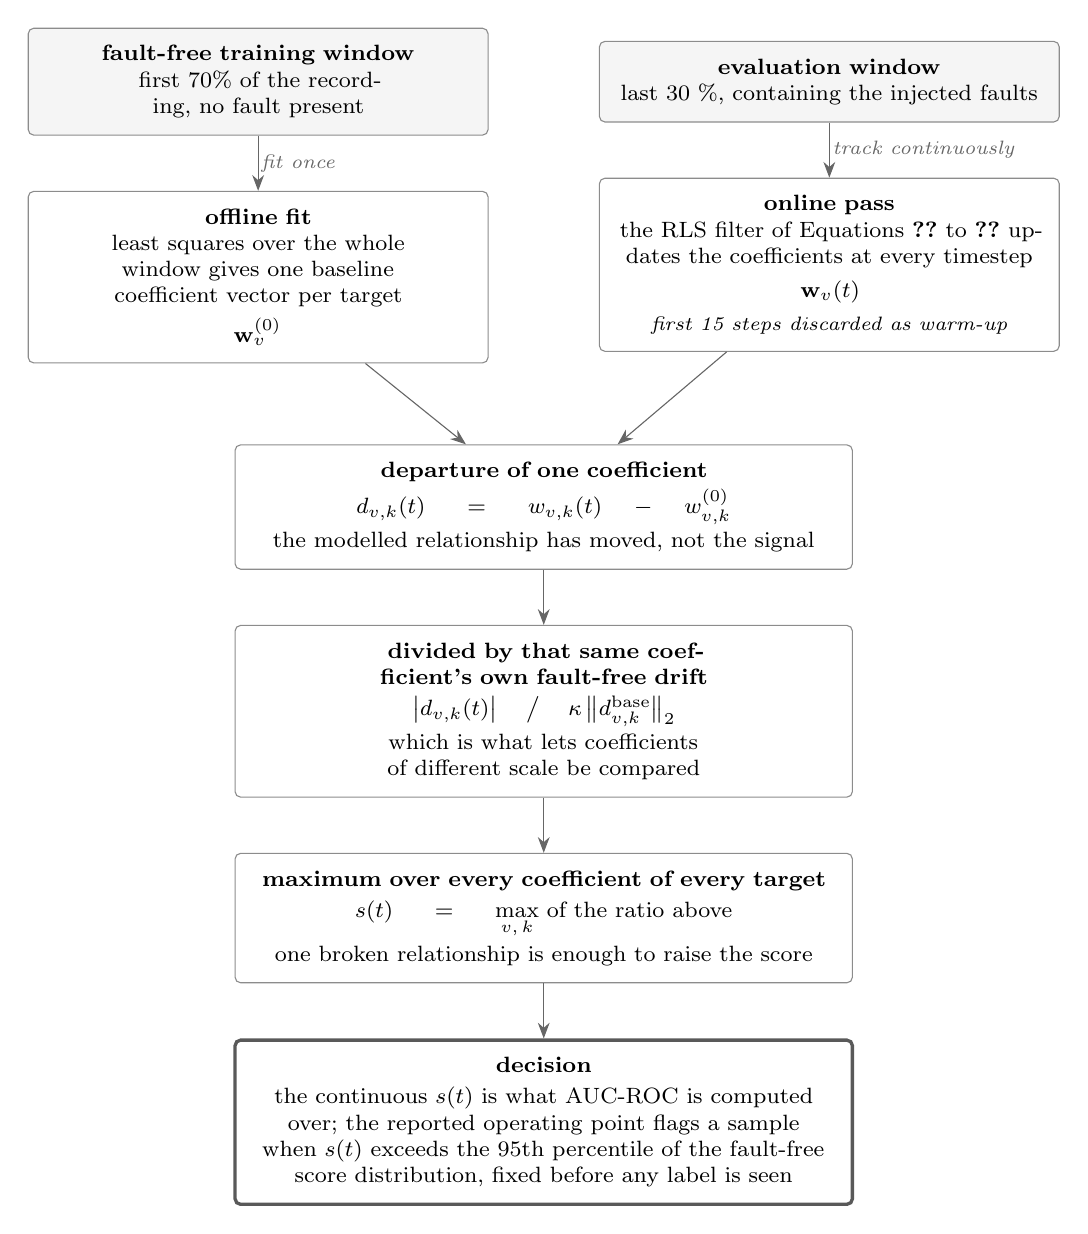
\begin{tikzpicture}[
  font=\small,
  dpbox/.style={draw=black!45, rounded corners=2pt, align=center,
                text width=54mm, inner sep=2.2mm, font=\footnotesize},
  dpsrc/.style={dpbox, fill=black!4},
  dpmid/.style={dpbox, text width=74mm},
  dpend/.style={dpbox, text width=74mm, draw=black!65, very thick},
  dparr/.style={-{Stealth[length=2mm]}, draw=black!60},
  dplbl/.style={font=\scriptsize\itshape, text=black!60, inner sep=1pt},
  node distance=7mm
]

% ---------------------------------------------- the two windows
\node[dpsrc] (train) {\textbf{fault-free training window}\\ first 70\%
  of the recording, no fault present};
\node[dpsrc, right=14mm of train] (evalwin) {\textbf{evaluation window}\\ last 30
 \%, containing the injected faults};

% ---------------------------------------------- the two passes
\node[dpbox, below=of train] (offline)
  {\textbf{offline fit}\\ least squares over the whole window gives one baseline
   coefficient vector per target\\[1mm] $\mathbf{w}^{(0)}_{v}$};
\node[dpbox, below=of evalwin] (online)
  {\textbf{online pass}\\ the RLS filter of Equations~\ref{eq:rls-gain}
   to~\ref{eq:rls-cov} updates the coefficients at every
   timestep\\[1mm] $\mathbf{w}_{v}(t)$\\[0.8mm]\scriptsize\itshape first 15 steps discarded as warm-up};

\draw[dparr] (train) -- node[dplbl, right] {fit once} (offline);
\draw[dparr] (evalwin) -- node[dplbl, right] {track continuously} (online);

% ---------------------------------------------- the difference
\coordinate (dpmerge) at ($(offline.south)!0.5!(online.south)$);
\node[dpmid, below=11mm of dpmerge] (diff)
  {\textbf{departure of one coefficient}\\[0.6mm]
   $d_{v,k}(t) \;=\; w_{v,k}(t) \;-\; w^{(0)}_{v,k}$\\[0.6mm]
   the modelled relationship has moved, not the signal};

\draw[dparr] (offline) -- (diff);
\draw[dparr] (online) -- (diff);


% ---------------------------------------------- normalisation
\node[dpmid, below=of diff] (norm)
  {\textbf{divided by that same coefficient's own fault-free drift}\\[0.6mm]
   $\bigl|d_{v,k}(t)\bigr| \;\big/\;
    \kappa\,\bigl\lVert d^{\mathrm{base}}_{v,k}\bigr\rVert_2$\\[0.6mm]
   which is what lets coefficients of different scale be compared};
\draw[dparr] (diff) -- (norm);

% ---------------------------------------------- the maximum
\node[dpmid, below=of norm] (agg)
  {\textbf{maximum over every coefficient of every target}\\[0.6mm]
   $s(t) \;=\; \displaystyle\max_{v,\,k}$ of the ratio above\\[0.6mm]
   one broken relationship is enough to raise the score};
\draw[dparr] (norm) -- (agg);

% ---------------------------------------------- the decision
\node[dpend, below=of agg] (flag)
  {\textbf{decision}\\[0.6mm]
   the continuous $s(t)$ is what AUC-ROC is computed over; the reported
   operating point flags a sample when $s(t)$ exceeds the 95th percentile
   of the fault-free score distribution, fixed before any label is seen};
\draw[dparr] (agg) -- (flag);

\end{tikzpicture}
}
%        \caption{...}
%        \label{fig:drift-pipeline}
%      \end{figure}
%
%  Why this figure exists.
%
%  Equations 3.1 to 3.4 give the recursive least squares update: how one
%  coefficient moves from one timestep to the next. They do not show the
%  thing the detector is built on, which is that two passes are run over
%  two disjoint windows and their coefficients are differenced. A reader
%  can follow every equation in Chapter 3 and still not know that w^(0)
%  comes from an offline fit on the training split while w(t) comes from
%  an online pass over the evaluation split, nor that the ratio is taken
%  per coefficient before the maximum is taken across them.
%
%  STYLE NAMES, because the first version of this figure would not
%  compile. Every style below is prefixed `dp'. The first version named
%  one of them `out', which is a reserved TikZ key -- it is the outgoing
%  angle in `to[out=30,in=150]' -- so `\node[out, ...]' was read as the
%  key /tikz/out with no value, and the rest of the picture unravelled
%  from there. `in', `at', `to', `pos', `scale' and `shift' are reserved
%  in the same way. A prefix costs nothing and rules the whole class of
%  collisions out.
%
%  LAYOUT: placement is relative throughout, via positioning's below=of
%  and right=of, so the boxes cannot overlap however the text inside them
%  reflows.
%=======================================================================
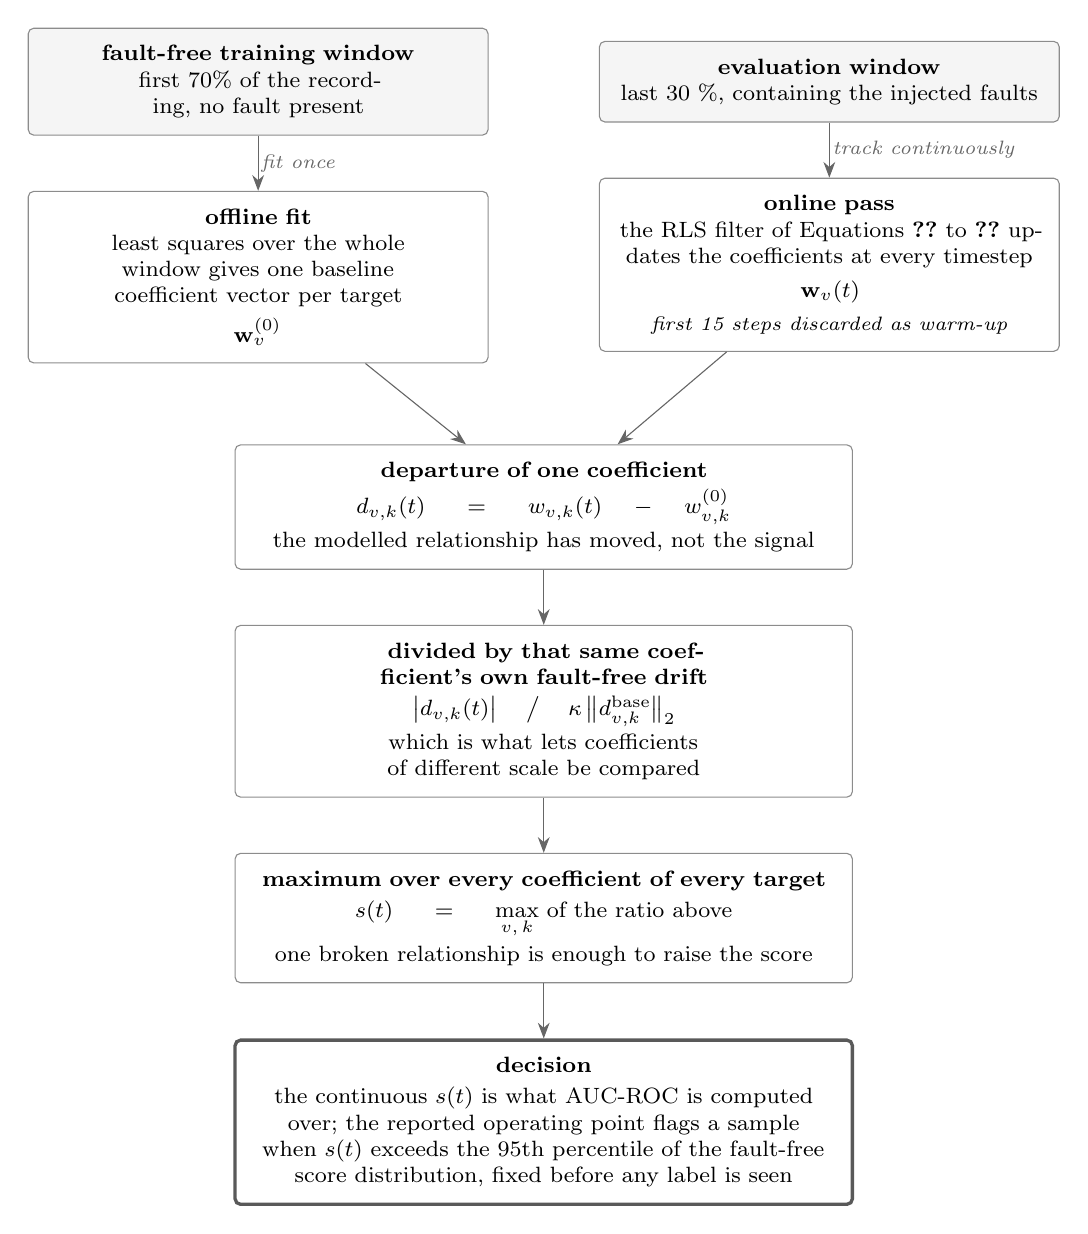
\begin{tikzpicture}[
  font=\small,
  dpbox/.style={draw=black!45, rounded corners=2pt, align=center,
                text width=54mm, inner sep=2.2mm, font=\footnotesize},
  dpsrc/.style={dpbox, fill=black!4},
  dpmid/.style={dpbox, text width=74mm},
  dpend/.style={dpbox, text width=74mm, draw=black!65, very thick},
  dparr/.style={-{Stealth[length=2mm]}, draw=black!60},
  dplbl/.style={font=\scriptsize\itshape, text=black!60, inner sep=1pt},
  node distance=7mm
]

% ---------------------------------------------- the two windows
\node[dpsrc] (train) {\textbf{fault-free training window}\\ first 70\%
  of the recording, no fault present};
\node[dpsrc, right=14mm of train] (evalwin) {\textbf{evaluation window}\\ last 30
 \%, containing the injected faults};

% ---------------------------------------------- the two passes
\node[dpbox, below=of train] (offline)
  {\textbf{offline fit}\\ least squares over the whole window gives one baseline
   coefficient vector per target\\[1mm] $\mathbf{w}^{(0)}_{v}$};
\node[dpbox, below=of evalwin] (online)
  {\textbf{online pass}\\ the RLS filter of Equations~\ref{eq:rls-gain}
   to~\ref{eq:rls-cov} updates the coefficients at every
   timestep\\[1mm] $\mathbf{w}_{v}(t)$\\[0.8mm]\scriptsize\itshape first 15 steps discarded as warm-up};

\draw[dparr] (train) -- node[dplbl, right] {fit once} (offline);
\draw[dparr] (evalwin) -- node[dplbl, right] {track continuously} (online);

% ---------------------------------------------- the difference
\coordinate (dpmerge) at ($(offline.south)!0.5!(online.south)$);
\node[dpmid, below=11mm of dpmerge] (diff)
  {\textbf{departure of one coefficient}\\[0.6mm]
   $d_{v,k}(t) \;=\; w_{v,k}(t) \;-\; w^{(0)}_{v,k}$\\[0.6mm]
   the modelled relationship has moved, not the signal};

\draw[dparr] (offline) -- (diff);
\draw[dparr] (online) -- (diff);


% ---------------------------------------------- normalisation
\node[dpmid, below=of diff] (norm)
  {\textbf{divided by that same coefficient's own fault-free drift}\\[0.6mm]
   $\bigl|d_{v,k}(t)\bigr| \;\big/\;
    \kappa\,\bigl\lVert d^{\mathrm{base}}_{v,k}\bigr\rVert_2$\\[0.6mm]
   which is what lets coefficients of different scale be compared};
\draw[dparr] (diff) -- (norm);

% ---------------------------------------------- the maximum
\node[dpmid, below=of norm] (agg)
  {\textbf{maximum over every coefficient of every target}\\[0.6mm]
   $s(t) \;=\; \displaystyle\max_{v,\,k}$ of the ratio above\\[0.6mm]
   one broken relationship is enough to raise the score};
\draw[dparr] (norm) -- (agg);

% ---------------------------------------------- the decision
\node[dpend, below=of agg] (flag)
  {\textbf{decision}\\[0.6mm]
   the continuous $s(t)$ is what AUC-ROC is computed over; the reported
   operating point flags a sample when $s(t)$ exceeds the 95th percentile
   of the fault-free score distribution, fixed before any label is seen};
\draw[dparr] (agg) -- (flag);

\end{tikzpicture}
}
  \caption[How a coefficient drift score is computed]{How a coefficient drift score is computed. The two windows are disjoint and the two passes are separate: the baseline coefficients are fitted offline on the fault-free training split, while the online filter tracks the coefficients across the evaluation split. Drift is their difference, taken per coefficient and normalised by that same coefficient's fault-free variation before the maximum is taken over all of them. The order of those last two operations is what makes a single broken relationship sufficient to raise the score. Every constant shown is the one the pipeline applies, and each is tabulated in Appendix~\ref{app:hyperparameters}.}
  \label{fig:drift-pipeline}
\end{figure}

Figure~\ref{fig:drift-pipeline} sets the mechanism out in one place. Equations~\ref{eq:rls-gain} to~\ref{eq:rls-cov} describe how a single coefficient moves from one timestep to the next; what they do not show is that two passes are run over two disjoint windows and their coefficients are then differenced. The baseline vector comes from the offline fit of the previous block, the tracked vector from the online pass, and the score is built from the gap.

\paragraph{Why drift and not residual magnitude.} The block rests on a premise that can be stated plainly and is testable. A detector whose state is the size of the residual cannot distinguish a mechanism breaking from a mechanism whose inputs have merely rescaled, because both make the observed values move. Coefficient drift tracks the integrity of the modelled relationship instead of the size of its error, and a rescaling that leaves the relationship intact leaves the coefficients where they were. The premise is not assumed here. It is verified against a controlled construction whose answer is known independently. A genuine structural break returns a mean drift of 4.1707; an amplitude rescaling that leaves the relationship intact returns 0.0002. Four orders of magnitude separate them, and a reconstruction metric separates them by nothing at all, because both move the observed values. Chapter~\ref{ch:experimental_setup} reports that check alongside the others, and Chapter~\ref{ch:results} measures the consequences on real data.

\paragraph{The decision rule.} An anomaly is declared when the score exceeds the 95th percentile of the drift distribution computed exclusively on held-out fault-free data. The rule is uniform across every configuration and it is label-blind by construction: the pipeline rejects threshold tuning against evaluation labels, which fits the operating point to the very faults being evaluated. The consequence is a fixed false-positive budget for every model, which is what gives the performance comparisons of Chapter~\ref{ch:results} a consistent basis.

\paragraph{Assumptions.} Scoring assumes the baseline vectors describe a healthy plant, and inherits everything the fit assumed. It assumes the fault-free drift used to set $\kappa$ and the threshold is representative of fault-free operation generally, so that a novel but benign operating regime is not scored as a fault. And it assumes a fault is expressed in the coefficients of at least one modelled mechanism, which is the substantive claim of the whole approach: a fault that changes no discovered relationship is invisible to this detector no matter how large it is.

%-----------------------------------------------------------------------
\section{Block Five: Attribution}
\label{sec:method-attribution}
\label{sec:bg-attribution}

\paragraph{Input and output.} The block receives the per-target drift vectors produced by the online pass, collected over two windows: the window in which the anomaly was flagged, and the fault-free baseline window. It emits a ranking of the monitored variables. The detection score says that something broke; this ranking says where to look.

The quantity ranked is the per-target drift norm $a_v(t)$ defined above, written $a_{:,i}$ when collected over the timesteps of a window for variable $i$. Two ranking rules are built from it and the pipeline uses both, in different places.

\paragraph{The normalised rule.} The attribution score for variable $i$ is the root mean square of its drift over the anomaly window, divided by the root mean square of the same quantity over the fault-free baseline window,
\[
  A_i = \frac{\operatorname{RMS}_{\text{attack}}\!\left(a_{:,i}\right)}
             {\max\!\left(E_i,\; 10^{-8}\right)},
  \qquad
  E_i = \operatorname{RMS}_{\text{baseline}}\!\left(a_{:,i}\right).
\]
The small constant is a floor on the denominator and not an additive smoothing term; it prevents division by a vanishing baseline for a variable that is effectively static. The ratio is length-independent, so a score of one means a variable is drifting exactly as much as it does under normal operation. This rule suits a system whose variables span very different intrinsic amplitudes, since a raw norm would let naturally noisy channels dominate the ranking whether or not their mechanisms had altered. What it isolates is the relative degradation of a mechanism, irrespective of the signal's native scale.

\paragraph{The unnormalised rule.} The second rule drops the baseline division and reduces the drift over the anomaly window directly,
\[
  A_i = \lVert a_{:,i} \rVert_2 .
\]
The norm is taken over time for a single variable, not over variables at a single time. This rule is retained for parity with the reference implementation wherever that reference defines the evaluation protocol, and it suits a system in which a genuinely quiet channel is quiet because nothing drives it. Dividing by a very small baseline confers an enormous advantage on such a channel and can displace the correct attribution entirely, which is not a hypothetical failure: Chapter~\ref{ch:results} exhibits it.

\paragraph{Which rule applies where.} The choice is made per domain and is declared in Section~\ref{sec:ranking-rule}, because it depends on the variance profile of the instrumented system rather than on anything methodological. One robotics fault settles the point. Under the raw norm the joint attack attributes to KneePicthTemp, the temperature the documented requirement names; under the normalised rule the same data returns LedEarR3 and LedEarL3, which carry the twelfth and thirteenth smallest fault-free baselines of 244 variables at 0.0268 against KneePicthTemp's 7.5380 at rank 238. Dividing by a baseline that small hands two quiet sensors a 281-fold advantage and displaces the correct attribution outright. Neither rule dominates, which is why the choice is made per domain and declared. Within a domain the rule is identical across all nine configurations, so within-domain comparisons are strictly like-for-like. Across domains they are not, and attribution rankings are therefore never compared between domains anywhere in this thesis.

One detail of the reduction has to be stated because it changes how a ranking must be read. Some configurations take the $L_2$ norm of the drift vector and others its root mean square, which is that norm divided by $\sqrt{T}$ for a window of $T$ timesteps. Since $T$ is a property of the window and not of the variable, the two differ by a factor constant across every variable being ranked, so they induce the same ordering and the same top entries. The consequential difference between the two rules is the division by $E_i$, which does vary by variable and does change the ranking. The choice of reduction does not.

\paragraph{Depth.} Attribution depth is held constant across every configuration. The ranking itself covers every monitored target; the per-anomaly figures plot the fifteen highest-scoring variables, or all of them where a domain monitors fewer; and the tables report the three highest, which is the depth at which every attribution result in this thesis is stated.

\paragraph{Assumptions.} The block assumes that the target whose coefficients moved most is the target nearest the fault, which is a strong assumption in a system with feedback, since a controller compensating for an upstream fault can produce the largest drift some distance from the cause. The robot's LED attack is that case, and the pipeline surfaces the downstream victim rather than the attacked channel: TabletTouchX, which ranks 78th of 249 sensors by raw standardised deviation, is returned first in all nine configurations. Whether that counts as the root cause or as one step removed from it is a question this assumption decides in advance. It assumes the drift observed during the anomaly window is attributable to the anomaly, which requires the window to be correctly located. And it assumes the monitored variable set contains something close to the root cause; a fault in an uninstrumented component can only ever be attributed to whichever measured mechanism it disturbed most.

\chapter{Experimental Setup and Dataset}
\label{ch:experimental_setup}

\section{Introduction}
Comparing a causal detector against a deep learning one is only worth doing if the comparison is controlled, and the usual failure is not a wrong result but an uninterpretable one. Where two methods differ in their preprocessing, their subsampling, their scaling or the way their threshold is set, the difference in their scores cannot be assigned to any of those things in particular, and the reported gap measures the experimental setup as much as it measures the algorithms.

The framework here is built around one constraint: everything downstream of the discovery step is held identical. All 27 causal configurations and all three deep learning baselines run through the same label-blind evaluation pipeline.

Three third-party implementations supply the discovery step. PCMCI is run through tigramite~\cite{runge2023tigramite}, GES through causal-learn~\cite{zheng2024causallearn}, and CAM-UV through lingam~\cite{ikeuchi2023lingam}. The regression variants, the ridge estimator, the polynomial expansion and the random Fourier feature map are standard implementations; the recursive least squares filter, the drift score, the thresholding rule and the attribution ranking are written for this pipeline. Discovery runs at a significance level of $\alpha = 0.05$ throughout, and PCMCI derives its maximum lag per domain from the frequency content of the signal, $\tau_{\max} = \lfloor f_{\max} / \bar{f} \rfloor$. The complete parameter set, including the per-domain forgetting factor $\lambda$, the tolerance multiplier $\kappa$, the ridge penalty and the subsampling rates, is tabulated in Appendix~\ref{app:hyperparameters}.

\label{sec:setup-lag}
One consequence of that derivation is worth recording here, because a later argument depends on it. PCMCI is free to place a parent at any lag from zero upward, and the minimum is left at the library default of zero, so a contemporaneous relationship is tested on the same footing as a lagged one. It overwhelmingly wins. Measured against the cached graphs under the pipeline's own sparsification rule and its lag-ordered three-parent cap, 100.0\% of the parent slots PCMCI's regressions retain on Healthcare and on Robotics sit at lag zero, and 98.7\% do on Industrial. On this pipeline PCMCI is therefore not the algorithm regressing each variable on its own past; it is the one most reliant on the present.

\section{Dataset Provenance and Characteristics}
To validate the generalisability and domain-specificity of the causal anomaly detection pipeline, experiments were conducted across three distinct environments: cyber-physical, biological, and industrial. Table~\ref{tab:datasets} places the three side by side before any of them is described in detail. They are not comparable in shape. The robot recording is wide and short, the electrocardiogram corpus is narrow and long, and the plant simulation sits between the two on both counts while carrying an evaluation split that is almost entirely faulty. Those differences govern a good deal of what Chapter~\ref{ch:results} reports, which is why they are gathered here at the outset.

\begin{table}[htbp]
  \centering
  \small
  \caption[The three evaluation datasets compared]{The three evaluation datasets compared. The robotics variable counts are the recorded columns and the number still varying once constant channels are dropped and the series is subsampled; the healthcare counts are the recorded leads and the subset that is algebraically independent of the rest. Fault-free samples are the observations the best causal configuration in each domain performs discovery on, at that configuration's own subsampling rate, and are taken from Table~\ref{tab:baseline_parity}. Anomaly prevalence is the positive rate of each evaluation split as scored by the parameter-free control of Section~\ref{sec:trivial-control}.}
  \label{tab:datasets}
  \begin{tabularx}{\textwidth}{@{}l
      >{\raggedright\arraybackslash}X
      >{\raggedright\arraybackslash}X
      >{\raggedright\arraybackslash}X@{}}
    \toprule
     & Robotics (Pepper) & Healthcare (PTB-XL) & Industrial (TEP) \\
    \midrule
    Monitored variables
      & 255 recorded, 244 after subsampling
      & 12 leads, 8 of them independent
      & 52 \\[0.35em]
    Fault-free samples
      & 274
      & 5{,}000
      & 500 \\[0.35em]
    Anomaly classes
      & 3
      & 20
      & 20 \\[0.35em]
    Anomaly prevalence
      & 0.5795
      & 0.5717
      & 0.9524 \\[0.35em]
    Nature of the faults
      & attacks injected into the control software of a live robot
      & cardiac pathology recorded from patients and labelled by a clinician
      & process disturbances introduced into a plant simulator \\
    \bottomrule
  \end{tabularx}
\end{table}

The fault column is the row that matters most for how the results are read. Only one of the three domains carries faults that were neither injected nor simulated, and it is also the domain where the detector has least raw amplitude to work with.

\subsection{The Cyber-Physical Domain: SoftBank PEPPER Robot}
The primary benchmark for this research is derived from the SoftBank Pepper humanoid robot, representing a highly dynamic, deterministic cyber-physical system. The raw dataset comprises high-frequency telemetry across 255 distinct variables, including kinematic sensors, hardware diagnostics, and software states. Three counts follow from that recording and the thesis quotes each of them, so they are separated here. Six variables never change during fault-free operation, leaving 249 that carry information; this is the population the model-free deviation ranking in Chapter~\ref{ch:results} works over. Subsampling to the discovery resolution of every 74th sample renders five more constant, so the causal graphs are learned over 244. Each number is correct for what it counts, and none is the raw sensor total.

One property of the export reaches the attribution figures, so it is recorded here. Eighteen sensor names occur twice, and in every one of the eighteen cases the two channels carry different readings, so they are distinct physical sensors that share a label, and not a duplicated column. They are disambiguated with a numeric suffix on load, which is why a bar in the robotics attribution plots is labelled \texttt{LaserF01X.1}.

The evaluation focuses on three documented cyber-physical attack vectors:
\begin{itemize}
    \item \textbf{\texttt{LedsControl}:} A software-level manipulation directly targeting the visual feedback hardware.
    \item \textbf{\texttt{JointControl}:} A physical manipulation resulting in a mechanical stress attack, driven by excess motor strain leading to elevated temperatures.
    \item \textbf{\texttt{WheelsControl}:} An attack manipulating the locomotion and gyroscope subsystems.
\end{itemize}

\subsection{The Healthcare Domain: PTB-XL ECG}
PTB-XL is a clinical electrocardiography corpus released through PhysioNet~\cite{wagner2020ptbxl,goldberger2000physionet}. Each record is a short resting electrocardiogram from one patient, annotated by a cardiologist, and this study uses the low-resolution release of each signal.

What the twelve channels record is one quantity seen from twelve directions. Depolarisation and repolarisation of the cardiac muscle produce a travelling electrical wavefront, and at the body surface that wavefront behaves approximately as a single time-varying dipole. A lead is a potential difference between electrode positions, which makes it a projection of that dipole onto one axis. Six limb leads (I, II, III, aVR, aVL, aVF) are derived from electrodes on the two arms and the left leg and view the heart in the frontal plane. Six precordial leads (V1 to V6) come from electrodes placed in sequence across the chest wall and view it in the transverse plane, from the right ventricle round to the lateral wall of the left. Twelve channels, one source.

The primary evaluation on the PTB-XL ECG dataset uses all 12 standard leads. Four of them (III, aVR, aVL, aVF) are exact linear functions of the others governed by Einthoven's and Goldberger's equations~\cite{malmivuo1995bioelectromagnetism,goldberger1942augmented}. Because causal discovery algorithms cannot distinguish algebraic definitions from biological mechanisms, a secondary robustness check was executed restricting the data strictly to the 8 algebraically independent leads. This ablation quantifies how much of the model's baseline performance was derived from exploiting these mathematical dependencies.

The dataset's diagnostic annotations roll up into five superclasses: a normal electrocardiogram, myocardial infarction, ST/T change, conduction disturbance and hypertrophy. Every one of the four abnormal superclasses is present among the records used here as anomaly classes. They include infarctions in the inferior, anteroseptal and lateral territories, non-diagnostic and non-specific ST/T abnormalities, anterior and posterior fascicular block, incomplete right bundle branch block, non-specific intraventricular conduction disturbance, and left and right ventricular hypertrophy. Several records carry a rhythm statement instead of, or alongside, a diagnostic one, atrial flutter and atrial fibrillation being the common cases, and the diagnostic superclasses do not cover those at all.

This is the domain where the case for a relational detector is easiest to state. Absolute amplitude in any single lead is a poor discriminator: it moves with electrode placement, chest wall thickness, body position and recording gain, and it varies between healthy people by more than several pathologies shift it. What identifies a condition is the pattern across leads. Infarction shows ST elevation in the leads that face the injured wall together with reciprocal depression in those facing away, so the sign of the relationship between two channels is the finding and the size of either one is not. Conduction disturbance changes the order and the relative timing of the deflections rather than their height. Hypertrophy is read from ratios, such as how the R wave grows from one precordial lead to the next. A detector that watches each channel's amplitude on its own has no access to any of this. One that tracks how each lead is predicted from the others does.

\subsection{The Industrial Domain: Tennessee Eastman Process}
The Tennessee Eastman Process (TEP) is a simulation of a real chemical plant, published by Downs and Vogel as an open control problem with the proprietary chemistry disguised behind lettered components~\cite{downs1993tep}. Four gaseous reactants are fed into a reactor, where exothermic and irreversible gas-phase reactions form two liquid products and a byproduct. An inert component enters with one of the feeds and accumulates, so the plant cannot be run closed.

The plant has five unit operations and the fault behaviour of all of them is observable. Reactor effluent leaves as vapour and is cooled through a condenser into a vapour-liquid separator. The uncondensed overhead from the separator is returned to the reactor feed by a recycle compressor, and a purge stream bleeds off the inert and the byproduct before they build up. Liquid from the separator passes to a stripper, where the light reactants still dissolved in it are stripped out with one of the feed streams and returned to the process; the stripper bottoms are the product. Two loops therefore close around the reactor, which is what makes the process a useful test case: a disturbance anywhere in the recycle path comes back to its own origin.

The 52 variables used here combine the plant's process measurements, which are flows, pressures, levels, temperatures and composition analyses taken around the reactor, the separator and the stripper, with the manipulated variables through which the control loops act on the valves. Both sides of the control loop are visible, and that is the reason a fault here need not show up as a large excursion in any measurement. A regulatory controller that is doing its job absorbs a disturbance by moving a valve, so the measured variable is held near setpoint and the evidence of the fault sits in the changed relationship between the two.

The twenty fault classes are the disturbances the original specification defines, simulated and released as labelled runs by Rieth et al.~\cite{rieth2017tepdata}. Most are step changes that shift a quantity to a new level and hold it there: the composition of a feed stream changes, or the inlet temperature of a cooling water supply moves. Several are random variations in the same quantities, which leave the mean where it was and alter only the variability, and these are much harder to see in a single channel. One is a slow drift in the reaction kinetics, which moves the plant gradually rather than at an instant, so there is no onset edge to detect. Two are sticking valves, one on the reactor cooling water and one on the condenser cooling water, where the actuator no longer tracks the command it is given. The remaining five the specification records only as unknown: the simulator injects them and does not say what they are. Each faulty run also begins in normal operation and the disturbance is introduced part of the way in, which is why the faulty files are trimmed to the post-onset window before they are scored.

Under the unified protocol, applying a 70/30 train-evaluation split reduced the discovery regime to merely 35 samples for 52 variables at a subsampling rate of $k=10$. This severely limits statistical power during the causal discovery phase. Table~\ref{tab:tep-power} quantifies the effect directly: holding the algorithm fixed and varying only the subsampling rate, the recovered graph density rises from 0.0238 at 35 samples to 0.1112 at 350. The sparsity of the industrial graphs is therefore a consequence of the sample count instead of a property of the process.

% GENERATED by Thesis/tools/make_tables.py -- do not edit by hand.
% Every figure below is read from a CSV written by the pipelines.
\begin{table}[htbp]
\centering
\caption[Discovery sample-count sweep over the Tennessee Eastman training window]{Discovery sample-count sweep over the Tennessee Eastman training window. The graph densifies monotonically as samples grow, which identifies the sparsity seen under the evaluation protocol as absent statistical power and not a property of the process.}
\label{tab:tep-power}
\begin{tabular}{rrrrr}
\toprule
Subsample & Samples & Parent edges & Confounded pairs & Density \\
\midrule
10 & 35 \footnotesize(protocol) & 35 & 14 & 2.4\% \\
5 & 70 & 35 & 28 & 3.4\% \\
2 & 175 & 59 & 38 & 5.1\% \\
1 & 350 & 115 & 90 & 11.1\% \\
\bottomrule
\end{tabular}
\end{table}


\section{Data Preprocessing and Leakage Prevention}
For all domains, the contiguous multivariate time-series data was strictly partitioned chronologically into a 70\% fault-free training set and a 30\% evaluation set. Normalisation is Z-score standardisation. To prevent leakage, the mean and standard deviation were fitted only on the 70\% fault-free training split.

To manage computational intractability, temporal subsampling was applied. The subsampling rate $k$ is a property of the algorithm's internal policy, not a global property of the domain. While GES and CAM-UV were evaluated at a fixed $k=10$ across all domains, PCMCI selects its subsampling adaptively ($k=74$ for Robotics, $k=7$ for Healthcare, $k=1$ for Industrial). Computational limits also required capping GES and CAM-UV at 35 variables using a label-blind variance filter. Strictly matched algorithmic comparisons are therefore limited to the Healthcare and Industrial domains. Because the algorithms score different sample sets, paired significance testing between PCMCI and the other causal algorithms is untestable.

\subsection{Preprocessing the Discovered Graph: Sparsification}
Everything above prepares the data. One further preparation step is applied to the graph, between discovery and scoring, and it is a preprocessing step in exactly the same sense: the detector never sees the raw output of a discovery algorithm, only the edge set that survives this rule.

Graph density is controlled by a dual-constraint sparsification rule. An edge is retained only if it achieves statistical significance ($p < 0.05$) and its absolute effect size exceeds a domain-specific multiplier applied to the mean absolute effect size. This multiplier was fixed at 1.0 for the Healthcare and Robotics domains and at 0.0 for the Industrial domain, where the second condition is therefore satisfied unconditionally.

The two quantities entering this rule are not the same object for all three algorithms, and the difference is worth stating and not leaving for a reader to discover. PCMCI supplies genuine partial correlations from its ParCorr test, so the stored effect sizes span $[-0.948, 0.954]$ and the filter discriminates among them: 149 of 564 candidate healthcare edges survive it. GES and CAM-UV instead supply edge indicators. A CPDAG and a CAM-UV parent set carry adjacency, not a continuous strength, so every discovered edge is recorded with a value of exactly 1.0 alongside a synthetic $p$-value. For those two algorithms the significance test reduces to \emph{the edge was discovered}, and the effect-size filter (comparing 1.0 against the mean of a sparse indicator matrix) is satisfied by every edge without exception.

The practical consequence is measurable and small. Across all nine algorithm--domain configurations the effect-size filter removes edges in exactly one, PCMCI on healthcare, where it discards three of 66 variable pairs. Graph density is therefore determined by what each algorithm discovers, not by the filter applied afterwards.

\section{Anomaly Scoring and Label-Blind Thresholding}
The causal anomaly detection pipeline does not evaluate reconstruction error; it measures coefficient drift. Reconstruction error asks whether a specific sensor value is unusual, whereas coefficient drift asks whether the fundamental physical relationship between variables has broken.

For a target variable with a design vector (which explicitly includes the intercept) built from its causal parents, the model tracks the evolution of regression coefficients using Recursive Least Squares (RLS). Following a 15-step warm-up period, each coefficient's departure from its fault-free value is compared against a tolerance derived from how far that same coefficient drifts under normal operation, and the score at each timestep is the largest such ratio across every coefficient of every modelled target:
$$s(t) = \max_{v,\,k}\ \frac{\bigl| w_{v,k}(t) - w_{v,k}^{(0)} \bigr|}{\kappa \, \bigl\lVert d^{\text{base}}_{v,k} \bigr\rVert_2}$$
The per-domain tolerance $\kappa$ takes the values 1.2 on Robotics, 2.0 on Healthcare and 3.0 on Industrial, and is identical across all three algorithms within each domain. Appendix~\ref{app:hyperparameters} tabulates it alongside every other setting the pipeline applies, separating the values the audit holds identical across all 27 configurations from the few that vary by algorithm or by domain, so that a reader can check the uniformity claim rather than take it. Because each coefficient is divided by its own fault-free drift, the score is expressed in multiples of normal variation rather than in raw coefficient units, which is what makes it comparable across variables of very different scale.
The theoretical justification for prioritising coefficient drift over reconstruction error is empirically verified. During algorithmic validation, a genuine structural relationship break yielded a mean drift score of 4.1707, whereas an amplitude rescaling with an intact relationship yielded a score of merely 0.0002. A standard reconstruction metric cannot distinguish between these two scenarios, but the drift metric successfully separates them by four orders of magnitude. Table~\ref{tab:validation} reports this alongside the other numerical checks, each of which constructs a problem whose answer is known independently and confirms the implementation reaches it.

% GENERATED by Thesis/tools/make_tables.py -- do not edit by hand.
% Every figure below is read from a CSV written by the pipelines.
\begin{table}[htbp]
\centering
\small
\caption[Numerical validation of the detector against closed-form answers]{Numerical validation of the detector against closed-form answers. Each row constructs a problem whose result is known independently of the implementation and confirms that the implementation reaches it.}
\label{tab:validation}
\begin{tabularx}{\textwidth}{@{}Xl r@{}}
\toprule
Check & Quantity & Value \\
\midrule
RLS at $\lambda=1$ equals ordinary least squares & max $|w_{\mathrm{RLS}} - w_{\mathrm{OLS}}|$ & $7.478 \times 10^{-10}$ \\
RLS with forgetting, $\lambda = 0.995$ & estimate of a coefficient stepping to $2.5$ & 2.5004 \\
RLS without forgetting, $\lambda = 1$ & same coefficient, no forgetting & 1.2522 \\
Drift when the relationship breaks & mean drift after the change & 4.1707 \\
Drift when values are rescaled but the relationship holds & mean drift after the change & 0.0002 \\
Drift when nothing changes & mean drift, second half & 0.0008 \\
\bottomrule
\end{tabularx}
\end{table}


To binarise the continuous anomaly scores, a universal, label-blind threshold $\tau$ was instituted. For every evaluated model, $\tau$ is defined precisely as the 95th percentile of the score distribution generated from the held-out fault-free data, ensuring a 5\% False Positive Rate (FPR) budget.

\subsection{The Per-Domain Ranking Rule}
\label{sec:ranking-rule}

The attribution ranking of Section~\ref{sec:method-attribution} admits two reductions, and which one applies is a property of the domain rather than of the method. Robotics ranks by the raw $L_2$ norm of the attack-window drift, retained for parity with the reference implementation that defines this domain's evaluation protocol. Healthcare and Industrial divide that norm by each variable's own fault-free baseline. The choice follows the variance profile of the instrumented system, and it is not neutral: Appendix~\ref{app:full-results} shows that on one robotics fault the two rules return different variables, and says which sensors the normalised rule promotes and why.

\section{Baseline Architectures and Hyperparameter Protocol}
Three deep learning autoencoders (LSTM, Temporal Convolutional Network, and Transformer) were implemented. Each architecture underwent a systematic 12-configuration hyperparameter search ($h \in \{32, 64\}$, $l \in \{1, 2, 3\}$, $\alpha \in \{0.001, 0.01\}$) across all three domains. The optimal configuration was selected based strictly on minimising the Mean Squared Error (MSE) on a disjoint 15\% fault-free validation split, with early stopping to prevent overfitting.

\subsection{Post-hoc Attribution over the Baselines}
\label{sec:setup-shap}

The neural baselines carry the comparison for explanation as well as for
detection, so each trained autoencoder is also explained. Attribution is
computed with SHAP, using the gradient explainer because it supports the
convolutional and attention architectures where the deep explainer's layer
rules do not cover every operation, and the quantity explained is the
reconstruction error the detector thresholds. The explainer is given fifty
fault-free windows as its background distribution, and the attributions are
summed over the time axis of each window and averaged over the windows of the
fault, which leaves one magnitude per variable per anomaly class. That is the
same shape the causal pipeline's attribution produces, so the two can be scored
by one procedure.

This is run on all three datasets over the same anomaly classes the causal
pipeline is scored on: the three injected robot attacks, the twenty
electrocardiogram records and the twenty plant faults. Each domain's loader
reads its subsampling stride and its non-constant variable set from that
domain's own causal cache, so the baselines see the matrix the causal pipeline
saw. Without that the two families would be attributing over different
variables and the comparison would not mean anything.

That parity is exact against PCMCI and against PCMCI alone. PCMCI derives its
stride from the frequency content of each signal, and the loaders inherit it.
CAM-UV and GES fix their stride at ten whatever the signal, so they read a
different number of rows in every domain, and on the plant they see a tenth of
what the baselines see. Comparisons involving those two are therefore between
methods that did not observe the same data, which is stated here because
Section~\ref{sec:attribution} draws conclusions from them. On the plant the
faulty files are also trimmed to the post-onset window before attribution, as
the causal pipeline does, since the fault is injected 160 samples in and the
earlier samples are fault-free.

Two properties of the method bear on how its output is read. The background
sample is drawn at random, so the explainer is seeded, and the instability that
remains across seeds is reported in Section~\ref{sec:attribution} instead of
being suppressed. And the magnitudes arrive in the units of the input, which
makes them incomparable between panels until each is normalised by its own
total; Section~\ref{sec:attribution} does that before any figure is read across
architectures.

\subsection{The Trivial Control}
\label{sec:trivial-control}
To establish an absolute performance floor, a trivial statistical control was evaluated alongside the deep learning baselines. This parameter-free baseline simply calculates the mean absolute $z$-score of the input window, standardised against the fault-free training mean and standard deviation, and applies the identical 95th-percentile decision rule. This control establishes the floor against which the computationally expensive causal and neural pipelines must justify themselves: an advantage over it is evidence of a genuine algorithmic capability, and its absence indicates that the faults were detectable by gross amplitude alone.

\section{Evaluation Metrics}
\label{sec:metrics}

Detection performance is evaluated with the standard classification metrics derived from the confusion matrix (precision, recall and $F_1$) alongside the threshold-free AUC-ROC and AUC-PR. AUC-ROC is the primary metric throughout, because it evaluates the ordering of the anomaly scores across all thresholds and not the quality of one operating point. $F_1$ is reported at the fixed 95th-percentile threshold, and because that collapses the score distribution to a single cut, a configuration with the better AUC-ROC can return the worse $F_1$ if its score distribution happens to align unfavourably with that cut.

AUC-PR is reported for completeness but cannot be compared across domains. Anomaly prevalence ranges from 0.5717 on Healthcare to 0.9524 on Industrial, as Table~\ref{tab:datasets} records, and AUC-PR depends directly on the positive rate~\cite{davis2006prroc}, so a cross-domain comparison on that metric would describe the datasets instead of the algorithms.

Uncertainty over the single-run causal configurations is quantified with a moving-block bootstrap of 2000 draws~\cite{kunsch1989blockbootstrap}. Resampling contiguous blocks preserves the local dependence that an independent resample would destroy, and the block length is derived per series from its own length and is not fixed,
\[
  L = \max\!\left(2,\; \operatorname{round}\!\left(n^{1/3}\right)\right),
\]
with $n$ the number of scored samples. Each configuration is seeded from a CRC32 hash of its own output path, so intervals are reproducible without being identical across configurations.

For a direct comparison between two configurations evaluated on the same samples the pipeline uses DeLong's test~\cite{delong1988comparing}, which operates on the difference of the two AUC estimates. It is more sensitive than inspecting whether two intervals overlap, and for a specific reason: the variance of the difference is $\mathrm{Var}(A_1) + \mathrm{Var}(A_2) - 2\,\mathrm{Cov}(A_1, A_2)$, so when two scores are positively correlated, as they are when computed on identical samples, the difference is known more precisely than either score alone. Two configurations whose intervals overlap substantially can therefore still be separable.

Attribution is not scored per sample but per anomaly class, so neither of those instruments applies to it and a third is needed. Uncertainty on the attribution figures of Section~\ref{sec:attribution} comes from a cluster bootstrap over anomaly classes: 20{,}000 resamples, percentile interval, seeded once at the start of the run so the figures are reproducible. Whole classes are drawn with replacement and every cell belonging to a drawn class is carried with it, because the three regression variants of one algorithm on one fault are three correlated observations of one event and resampling them independently would return an interval too narrow to believe. Comparisons between two methods are made on the paired difference within each class, which removes the between-class variance that dominates here, some faults being easier to attribute than others for every method at once.

That interval is reported as a descriptive range and is not the decision rule, because at these sample sizes it cannot state its own level. Whether a percentile interval excludes zero is related to whether the classes agree in sign, but only in one direction: unanimity implies exclusion and exclusion does not imply unanimity, so the probability $2^{1-n}$ that all $n$ classes fall on the same side of a symmetric null bounds such a rule's false-positive rate from below without fixing it. A lower bound is worth having where it is large, and useless where it is small.

The decision rule is therefore an exact paired sign test on the class differences, with ties discarded. It has a level at every sample size, and its smallest attainable two-sided value on $n$ untied classes is exactly $2^{1-n}$ rather than merely at least that. The consequence is the binding constraint on two of the three domains. Those floors are the best a panel of that size can do, and ties push them higher still, since a tied class is discarded and the exponent runs on what survives. With the robot's three attack classes the smallest $p$ the design admits is therefore 0.25 at best, and with the plant's five documented actuators 0.0625 at best; in practice several of the plant's comparisons tie on three or four of their five classes and their real floor is 0.5 or 1. Neither panel reaches the 5\% level however large the observed difference, so neither is asked for a verdict. With the fourteen localisable cardiac classes the floor is $1.2 \times 10^{-4}$ before ties and no worse than $10^{-3}$ after them, so a verdict is available there whichever way the ties fall. The same arithmetic explains why the bootstrap bounds on the robot are worth nothing beyond description: with $3^3 = 27$ equally likely resamples the all-minimum draw carries $1/27 = 3.7\%$ of the mass, more than the 2.5\% the lower tail removes, so the reported interval is exactly the range of the three values.

Multiplicity is controlled rather than ignored. Section~\ref{sec:method-attribution} fixes the top-three ranking as the depth at which every attribution result in this thesis is stated, so the primary family is the three comparisons at that depth within a domain and Holm's step-down correction is applied across them. The remaining three depths are exploratory; they are reported uncorrected, labelled as such, and tabulated in full as Table~\ref{tab:attr-paired-full} rather than omitted, because choosing which depth to show after seeing what each one says is the failure Section~\ref{sec:rel-evaluation} names as this field's fourth.

\chapter{Results}
\label{ch:results}

\section{Headline comparison}

RQ1 asks which causal discovery algorithm gives the most effective anomaly detection under one shared protocol, and whether that ranking holds from one application domain to the next. Table~\ref{tab:main-results} presents the headline anomaly detection performance across 27 distinct causal discovery configurations, structured along three primary axes: the dataset domain, the underlying causal discovery algorithm, and the applied regression variant.
% GENERATED by Thesis/tools/make_tables.py -- do not edit by hand.
% Every figure below is read from a CSV written by the pipelines.
\begin{table}[htbp]
\centering
\small
\caption[Detection performance (AUC-ROC) for all 27 causal configurations]{Detection performance (AUC-ROC) for all 27 causal configurations. Rows are causal discovery algorithms, columns are regression variants, blocks are application domains. The best value within each domain is shown in bold.}
\label{tab:main-results}
\begin{tabular}{llrrr}
\toprule
Domain & Algorithm & Linear / Ridge $\uparrow$ & Polynomial $\uparrow$ & RBF + Ridge $\uparrow$ \\
\midrule
\multirow{3}{*}{Robotics (Pepper)} & PCMCI & 0.7825 & 0.8053 & \textbf{0.8752} \\
 & GES & 0.5906 & 0.6999 & 0.6516 \\
 & CAM-UV & 0.6497 & 0.6888 & 0.7818 \\
\midrule
\multirow{3}{*}{Healthcare (PTB-XL)} & PCMCI & 0.6181 & 0.5075 & 0.7147 \\
 & GES & \textbf{0.8114} & 0.7867 & 0.7620 \\
 & CAM-UV & 0.7861 & 0.7691 & 0.7692 \\
\midrule
\multirow{3}{*}{Industrial (TEP)} & PCMCI & 0.8860 & \textbf{0.9151} & 0.8495 \\
 & GES & 0.8407 & 0.8849 & 0.8994 \\
 & CAM-UV & 0.8428 & 0.8212 & 0.8922 \\
\bottomrule
\end{tabular}
\end{table}


No single detection paradigm wins across all three domains. Which one is ahead depends on the domain, and that dependence is the result rather than a complication of it. In the cyber-physical Robotics domain, the tuned neural baseline attains a higher point estimate than the optimal causal configuration (AUC-ROC 0.8856 versus 0.8752), although Section~\ref{sec:uncertainty} shows this ordering is not supported once sampling uncertainty is accounted for. In the Industrial domain the deep learning architectures win outright (AUC-ROC 0.9997), and the parameter-free trivial control also scores above the best causal pipeline (0.9286 versus 0.9151), an ordering Section~\ref{sec:uncertainty} likewise shows to be inseparable. The biological Healthcare domain is where the causal approach holds up: the causal pipeline achieves an AUC-ROC of 0.8114 against the tuned neural baseline (0.7077) and the trivial control (0.6136). This ordering rests on point estimates alone, since the causal and neural pipelines score different sample sets and therefore admit no paired significance test.

Table~\ref{tab:main-results} also carries the measurement RQ2 asks for, which is the second axis read down the columns, not across the rows. Of the nine algorithm--domain cells the RBF feature map takes five, the linear map two and the degree-three polynomial two. No variant dominates, and the pattern is not a property of the domain either: GES prefers a different variant in each of the three domains, taking the polynomial on robotics, the linear map on healthcare and RBF on industrial. Which regression family performs best therefore cannot be stated without naming both the algorithm and the domain, and the interaction is reported here rather than resolved. With one run per cell there is no within-cell variance and so no formal test of it, as Section~\ref{sec:disc-threats} records.

\subsection{Per-domain detail}
\label{sec:per-domain}

Precision, recall, F1 and AUC-ROC for every configuration on the cyber-physical Robotics domain are set out in Table~\ref{tab:detail-robotic}.
% GENERATED by Thesis/tools/make_tables.py -- do not edit by hand.
% Every figure below is read from a CSV written by the pipelines.
\begin{table}[htbp]
\centering
\footnotesize
\setlength{\tabcolsep}{3pt}
\caption[Complete detection metrics for the robotics domain]{Complete detection metrics for the robotics domain. The threshold is the 95th percentile of the fault-free score distribution, computed without reference to any anomaly label.}
\label{tab:detail-robotic}
\begin{tabular}{llrrrrrrrrrr}
\toprule
Algorithm & Variant & Thr. & TP $\uparrow$ & FP $\downarrow$ & TN $\uparrow$ & FN $\downarrow$ & Acc. $\uparrow$ & Prec. $\uparrow$ & Rec. $\uparrow$ & F1 $\uparrow$ & AUC $\uparrow$ \\
\midrule
\multirow{3}{*}{PCMCI} & Linear & 1.103 & 55 & 4 & 64 & 58 & 0.6575 & 0.9322 & 0.4867 & 0.6395 & 0.7825 \\
 & Poly-3 & 2.370 & 75 & 4 & 64 & 38 & 0.7680 & 0.9494 & 0.6637 & 0.7812 & 0.8053 \\
 & RBF & 2.450 & 77 & 4 & 64 & 36 & 0.7790 & 0.9506 & \textbf{0.6814} & 0.7938 & \textbf{0.8752} \\
\midrule
\multirow{3}{*}{GES} & Linear & 0.259 & 321 & 28 & 520 & 509 & 0.6103 & 0.9198 & 0.3867 & 0.5445 & 0.5906 \\
 & Poly-3 & 3.278 & 383 & 28 & 520 & 447 & 0.6553 & 0.9319 & 0.4614 & 0.6172 & 0.6999 \\
 & RBF & 0.426 & 421 & 28 & 520 & 409 & 0.6829 & 0.9376 & 0.5072 & 0.6583 & 0.6516 \\
\midrule
\multirow{3}{*}{CAM-UV} & Linear & 0.196 & 267 & 28 & 520 & 563 & 0.5711 & 0.9051 & 0.3217 & 0.4747 & 0.6497 \\
 & Poly-3 & 1.074 & 328 & 28 & 520 & 502 & 0.6154 & 0.9213 & 0.3952 & 0.5531 & 0.6888 \\
 & RBF & 0.150 & 565 & 28 & 520 & 265 & \textbf{0.7874} & \textbf{0.9528} & 0.6807 & \textbf{0.7941} & 0.7818 \\
\bottomrule
\end{tabular}
\end{table}


AUC-ROC and F1 disagree in this study because they answer different questions. AUC-ROC evaluates ranking across all possible thresholds, whereas F1 is reported at a single operating point: the 95th percentile of the fault-free score distribution, fixed before any attack label is seen.

The consequence is visible in the per-domain tables. Because the threshold fixes the false-positive rate at 5\% by construction, precision is nearly constant across all nine robotics configurations, ranging only from 0.9051 to 0.9528, while recall varies by a factor of two, from 0.3217 to 0.6814. F1 therefore moves almost entirely through recall, and reflects how well each score distribution happens to align with that particular cut-off and not how well the model ranks.

Seven rank inversions follow. The strongest configuration by AUC-ROC, PCMCI with RBF features at 0.8752, is marginally beaten on F1 by CAM-UV with RBF features at 0.7818, a configuration 0.093 lower in ranking ability. PCMCI linear/ridge, at 0.7825, loses on F1 to GES with RBF features at 0.6516, a gap of 0.13.

This is the intended cost of refusing to fit the threshold to test labels. F1 is reported as an achievable operating point, not a maximum, and AUC-ROC is treated as the primary measure of discriminative ability throughout.

The corresponding metrics for the biological Healthcare domain, over all twelve standard leads, are in Table~\ref{tab:detail-healthcare}. The eight-lead ablation is reported separately in Section~\ref{sec:eight-lead-ablation}.
% GENERATED by Thesis/tools/make_tables.py -- do not edit by hand.
% Every figure below is read from a CSV written by the pipelines.
\begin{table}[htbp]
\centering
\footnotesize
\setlength{\tabcolsep}{3pt}
\caption[Complete detection metrics for the healthcare domain]{Complete detection metrics for the healthcare domain. The threshold is the 95th percentile of the fault-free score distribution, computed without reference to any anomaly label.}
\label{tab:detail-healthcare}
\begin{tabular}{llrrrrrrrrrr}
\toprule
Algorithm & Variant & Thr. & TP $\uparrow$ & FP $\downarrow$ & TN $\uparrow$ & FN $\downarrow$ & Acc. $\uparrow$ & Prec. $\uparrow$ & Rec. $\uparrow$ & F1 $\uparrow$ & AUC $\uparrow$ \\
\midrule
\multirow{3}{*}{PCMCI} & Linear & 0.026 & 525 & 98 & 1848 & 2335 & 0.4938 & 0.8427 & 0.1836 & 0.3015 & 0.6181 \\
 & Poly-3 & 0.050 & 180 & 98 & 1848 & 2680 & 0.4220 & 0.6475 & 0.0629 & 0.1147 & 0.5075 \\
 & RBF & 0.034 & 1041 & 98 & 1848 & 1819 & 0.6011 & \textbf{0.9140} & 0.3640 & 0.5206 & 0.7147 \\
\midrule
\multirow{3}{*}{GES} & Linear & 0.033 & 711 & 73 & 1382 & 949 & \textbf{0.6719} & 0.9069 & \textbf{0.4283} & \textbf{0.5818} & \textbf{0.8114} \\
 & Poly-3 & 0.057 & 440 & 73 & 1382 & 1220 & 0.5849 & 0.8577 & 0.2651 & 0.4050 & 0.7867 \\
 & RBF & 0.044 & 602 & 73 & 1382 & 1058 & 0.6369 & 0.8919 & 0.3627 & 0.5156 & 0.7620 \\
\midrule
\multirow{3}{*}{CAM-UV} & Linear & 0.035 & 608 & 73 & 1382 & 1052 & 0.6388 & 0.8928 & 0.3663 & 0.5194 & 0.7861 \\
 & Poly-3 & 0.058 & 438 & 73 & 1382 & 1222 & 0.5843 & 0.8571 & 0.2639 & 0.4035 & 0.7691 \\
 & RBF & 0.049 & 513 & 73 & 1382 & 1147 & 0.6083 & 0.8754 & 0.3090 & 0.4568 & 0.7692 \\
\bottomrule
\end{tabular}
\end{table}


The divergence between AUC-ROC and F1 described above for Table~\ref{tab:detail-robotic} applies identically here, and for the same reason: the operating point is fixed by the fault-free distribution rather than chosen to maximise F1.

For the Industrial domain the complete configuration breakdown is Table~\ref{tab:detail-industrial}.
% GENERATED by Thesis/tools/make_tables.py -- do not edit by hand.
% Every figure below is read from a CSV written by the pipelines.
\begin{table}[htbp]
\centering
\footnotesize
\setlength{\tabcolsep}{3pt}
\caption[Complete detection metrics for the industrial domain]{Complete detection metrics for the industrial domain. The threshold is the 95th percentile of the fault-free score distribution, computed without reference to any anomaly label.}
\label{tab:detail-industrial}
\begin{tabular}{llrrrrrrrrrr}
\toprule
Algorithm & Variant & Thr. & TP $\uparrow$ & FP $\downarrow$ & TN $\uparrow$ & FN $\downarrow$ & Acc. $\uparrow$ & Prec. $\uparrow$ & Rec. $\uparrow$ & F1 $\uparrow$ & AUC $\uparrow$ \\
\midrule
\multirow{3}{*}{PCMCI} & Linear & 0.194 & 12536 & 40 & 756 & 3384 & 0.7952 & \textbf{0.9968} & 0.7874 & 0.8798 & 0.8860 \\
 & Poly-3 & 0.217 & 12598 & 40 & 756 & 3322 & 0.7989 & \textbf{0.9968} & 0.7913 & 0.8823 & \textbf{0.9151} \\
 & RBF & 0.347 & 11738 & 40 & 756 & 4182 & 0.7474 & 0.9966 & 0.7373 & 0.8476 & 0.8495 \\
\midrule
\multirow{3}{*}{GES} & Linear & 1.357 & 950 & 4 & 59 & 310 & 0.7627 & 0.9958 & 0.7540 & 0.8582 & 0.8407 \\
 & Poly-3 & 2.576 & 945 & 4 & 59 & 315 & 0.7589 & 0.9958 & 0.7500 & 0.8556 & 0.8849 \\
 & RBF & 3.060 & 1019 & 4 & 59 & 241 & \textbf{0.8148} & 0.9961 & \textbf{0.8087} & \textbf{0.8927} & 0.8994 \\
\midrule
\multirow{3}{*}{CAM-UV} & Linear & 1.061 & 962 & 4 & 59 & 298 & 0.7717 & 0.9959 & 0.7635 & 0.8643 & 0.8428 \\
 & Poly-3 & 2.579 & 865 & 4 & 59 & 395 & 0.6984 & 0.9954 & 0.6865 & 0.8126 & 0.8212 \\
 & RBF & 3.036 & 1001 & 4 & 59 & 259 & 0.8012 & 0.9960 & 0.7944 & 0.8839 & 0.8922 \\
\bottomrule
\end{tabular}
\end{table}


The same qualification applies. Note also that this evaluation set carries a 95.24\% anomaly prevalence, so AUC-PR is inflated by the class balance and threshold-independent AUC-ROC should be preferred when comparing configurations on this domain.

\section{Uncertainty}
\label{sec:uncertainty}

To account for the autocorrelation inherent in time-series data, uncertainty is quantified using a moving-block bootstrap and not the analytical Hanley--McNeil interval~\cite{hanley1982roc}. An i.i.d. resample destroys serial dependence and produces artificially narrow intervals, whereas the block bootstrap preserves temporal dynamics and yields honest confidence bounds.

Figure~\ref{fig:forest} plots all 27 intervals at once, which is what makes the argument of this section legible: the extent to which the intervals overlap is a property of the whole set and not of any row in it. Where an exact bound is wanted, Table~\ref{tab:bootstrap} in Appendix~\ref{app:full-results} lists every interval, with the analytical Hanley--McNeil bounds beside it for comparison.

\begin{figure}[htbp]
  \centering
  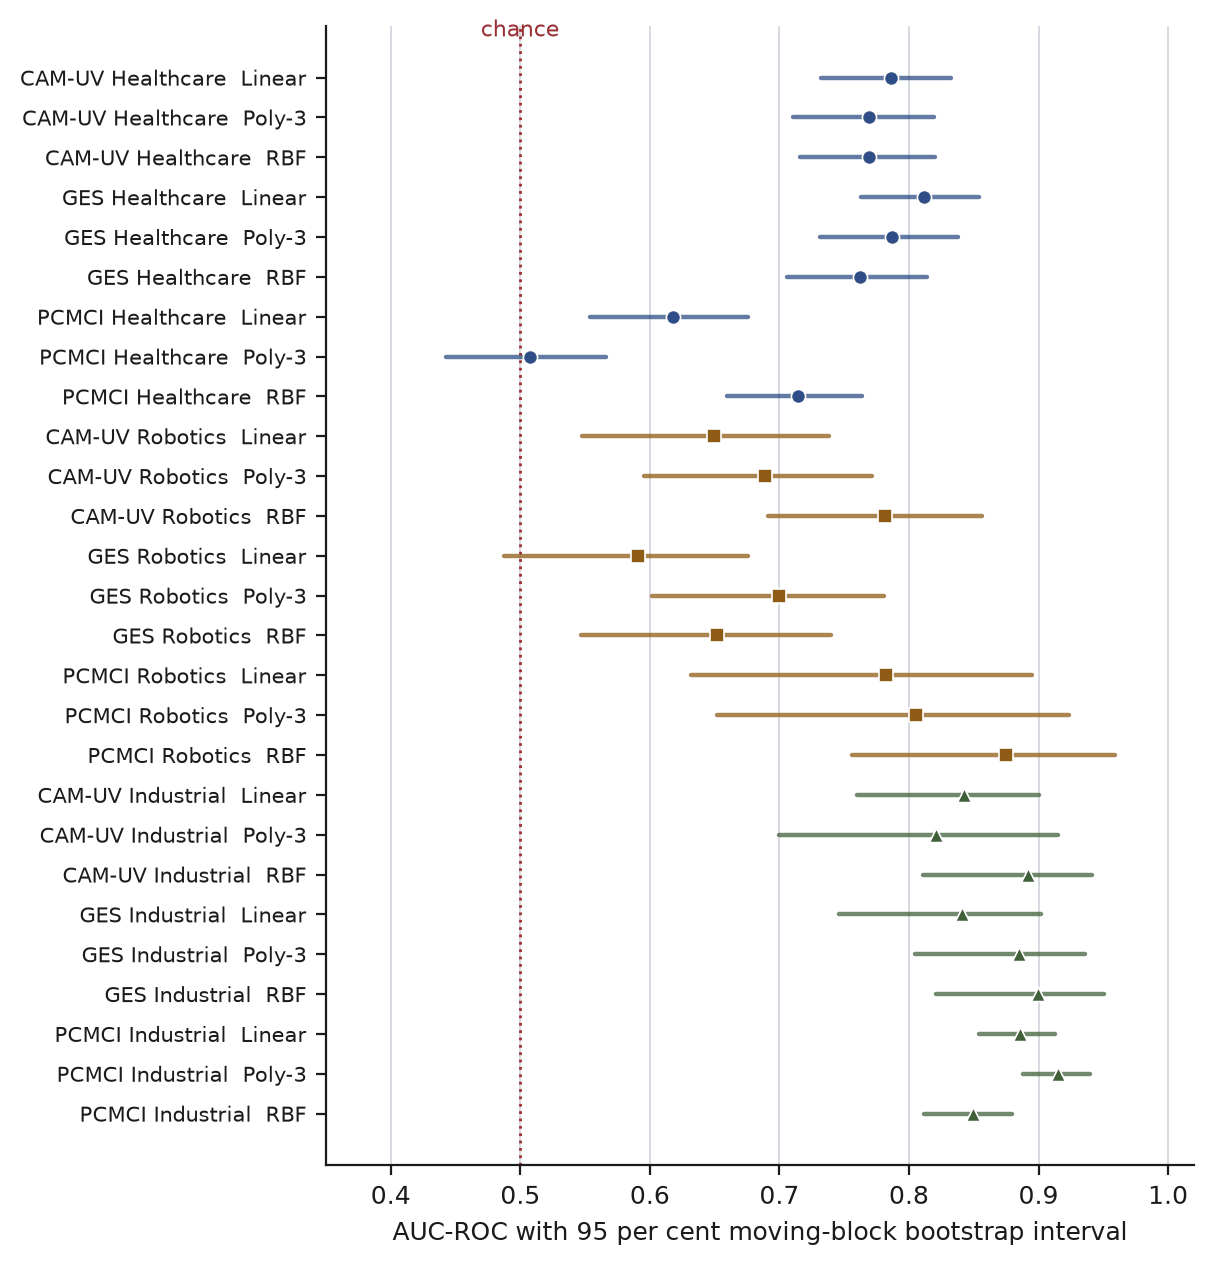
\includegraphics[width=0.86\textwidth]{fig_bootstrap_forest.png}
  \caption[Bootstrap intervals for all 27 causal configurations]{Bootstrap intervals for all 27 causal configurations, grouped by domain. Two intervals cross the chance line: PCMCI with polynomial features on healthcare, which sits almost exactly on it, and GES with linear features on robotics. The widest intervals in the study belong to PCMCI on robotics, which is also where its highest point estimate sits: 181 scored samples against 1{,}378 for the other two algorithms in that domain.}
  \label{fig:forest}
\end{figure}

Accounting for sample uncertainty via moving-block bootstrapping reveals that strict hierarchical rankings within the Robotics domain are statistically unsupported. The optimal causal configuration (PCMCI-RBF, AUC-ROC 0.8752) exhibits a wide 95\% confidence interval of [0.7559, 0.9587]. This interval, spanning 0.203, entirely encompasses the tuned neural baseline and heavily overlaps with multiple subsequent causal configurations. The sample size behind that interval is the reason, and it is a property of the configuration rather than of the domain: PCMCI scores robotics at its own coarser resolution and is therefore evaluated over 181 samples, where GES and CAM-UV are evaluated over 1{,}378. The widest intervals in the domain are consequently PCMCI's, and the configuration with the highest point estimate is also the one whose estimate is least precisely known. These models cannot be definitively ranked by point estimates alone. The intervals also expose configurations whose performance cannot be separated from chance, such as GES-Linear, whose interval of [0.4873, 0.6761] crosses 0.5.

The same test must be applied to the comparisons that run against this thesis as well as to those that run for it, and on the Industrial domain it changes what may be claimed. The parameter-free control scores 0.9286 there against 0.9151 for the best causal configuration, but that configuration's interval is $[0.8880, 0.9394]$ and the control's score falls inside it; the two also score different numbers of samples, so no paired test is available either. The control is therefore not shown to beat the causal pipeline on Industrial. What is shown is that the causal pipeline cannot be distinguished from a method with no learned parameters, which is the weaker statement and the one Section~\ref{sec:disc-when} relies on. By contrast the neural baselines at 0.9997 sit well outside that interval, so that ordering is separable and is reported as such.

It is critical to note, however, that overlapping confidence intervals are a weaker measure of separability than paired testing. While interval overlap indicates high marginal variance, paired significance testing via the DeLong method demonstrates that specific configurations on a shared sample set remain statistically distinct (PCMCI-RBF versus PCMCI-Linear, $p = 0.000011$), confirming that paired tests are required to evaluate model modifications measured on identical data.

Table~\ref{tab:delong-summary} reports what that test can and cannot reach across the whole grid. Each domain contributes 36 within-domain pairs, and exactly half of them are testable: a pair fails whenever PCMCI is on exactly one side of it, because PCMCI subsamples at its own rate and the two configurations then score different observations. Two PCMCI configurations share a sample set with each other and are testable, which is why the paragraph above can report one. The split is 54 testable against 54 unpairable, identically in all three domains, and it is not a property of the data but of the decision to treat the subsampling rate as belonging to each algorithm. Of the 54 that can be tested, 41 separate at the 5\% level, so the instrument is not weak where it applies; it simply does not reach the comparison RQ1 asks for. The full set is given as Table~\ref{tab:delong-full}.

% GENERATED by Thesis/tools/make_tables.py -- do not edit by hand.
% Every figure below is read from a CSV written by the pipelines.
\begin{table}[htbp]
\centering
\caption[Paired AUC comparisons by DeLong's test, by domain]{Paired AUC comparisons by DeLong's test, by domain. Every within-domain pair of the nine configurations is counted, so each domain contributes 36. A pair is testable only when both configurations score the same observations, which fails wherever PCMCI is on exactly one side of the comparison because it subsamples at its own rate; two PCMCI configurations share a sample set with each other and are testable, which is what makes the split 18 and 18 rather than 21 and 15. The unpairable column is the cost of treating the subsampling rate as a property of each algorithm and not as a pipeline constant.}
\label{tab:delong-summary}
\begin{tabular}{lrrrr}
\toprule
Domain & Comparisons & Testable $\uparrow$ & Unpairable $\downarrow$ & Significant $\uparrow$ \\
\midrule
Healthcare (ECG) & 36 & 18 & 18 & 14 \\
Industrial (TEP) & 36 & 18 & 18 & 12 \\
Robotics (Pepper) & 36 & 18 & 18 & 15 \\
\midrule
\textbf{All three} & \textbf{108} & \textbf{54} & \textbf{54} & \textbf{41} \\
\bottomrule
\end{tabular}
\end{table}


\section{Comparison against baselines}
\label{sec:baselines}

This section reports the measurements bearing on RQ3, which asks whether causal detectors outperform non-causal neural baselines of comparable capacity, and under what conditions. The parameter-free control is reported alongside them, because the condition turns out to be legible in its score. Table~\ref{tab:baselines} details the performance of the three deep learning autoencoders (LSTM, TCN and Transformer) following domain-specific hyperparameter tuning, alongside the parameter-free trivial statistical control. All models operate under the identical 95th-percentile label-blind decision rule.

The baselines are reported at a coarser grain than the causal configurations, and the reason is a matter of what was kept. Each autoencoder figure is a mean AUC-ROC over three seeds with its standard deviation, so Table~\ref{tab:baselines} gives no counterpart to the per-configuration confusion matrices of Section~\ref{sec:per-domain}: the per-seed true and false positive counts were not retained when the runs were aggregated, and they are not reconstructed here from the summary statistics that were.

One asymmetry in that protocol has to be declared, because it bears on the comparison the healthcare column is used to make. The autoencoders take their variable set and their scoring resolution from PCMCI's cached graph in every domain. On robotics and industrial that is also the resolution of the best causal configuration, so those columns compare like with like. On healthcare it is not: the strongest causal result is GES's, obtained at a coarser subsampling rate, so the fault-free recording yields 7{,}143 samples at the resolution the baselines work in and 5{,}000 at the one GES works in. The variable set is identical, all twelve leads in both cases, so the difference is one of resolution alone. Its direction is worth stating explicitly, since it runs against the thesis and not for it: the healthcare baselines are trained and evaluated on more data than the causal configuration they are compared against, so the causal margin reported in that column is measured against a better-resourced opponent, not a handicapped one. Table~\ref{tab:baseline_parity} sets out what each side was given in each domain, so that the declaration can be checked rather than taken on trust.
% GENERATED by Thesis/tools/make_tables.py -- do not edit by hand.
% Every figure below is read from a CSV written by the pipelines.
\begin{table}[htbp]
\centering
\small
\caption[Non-causal reference points, as AUC-ROC]{Non-causal reference points, as AUC-ROC. The neural autoencoders read the same variables and apply the same 95th-percentile fault-free threshold as the causal pipelines, and are reported as the mean over three seeds with the standard deviation across them. They run at PCMCI's scoring resolution in every domain, which matches the best causal configuration on robotics and industrial but not on healthcare. Table~\ref{tab:baseline_parity} sets out what each side was given in each domain, including the direction of that asymmetry, which runs against this thesis instead of for it. The trivial control is a parameter-free mean absolute $z$-score with no learned parameters at all. Bold marks the best value in each column, whichever family it belongs to.}
\label{tab:baselines}
\begin{tabular}{lccc}
\toprule
Method & Robotics $\uparrow$ & Healthcare $\uparrow$ & Industrial $\uparrow$ \\
\midrule
LSTM autoencoder & $0.8804 \pm 0.0032$ & $0.7077 \pm 0.0048$ & $0.9670 \pm 0.0006$ \\
TCN autoencoder & $\mathbf{0.8856 \pm 0.0051}$ & $0.6379 \pm 0.0038$ & $\mathbf{0.9997 \pm 0.0001}$ \\
Transformer autoencoder & $0.8139 \pm 0.0158$ & $0.6102 \pm 0.0332$ & $0.9988 \pm 0.0001$ \\
\midrule
Trivial control, mean $|z|$ & $0.8139$ & $0.6136$ & $0.9286$ \\
\midrule
Best causal configuration & $0.8752$ & $\mathbf{0.8114}$ & $0.9151$ \\
\bottomrule
\end{tabular}
\end{table}


% GENERATED by Thesis/tools/make_tables.py -- do not edit by hand.
% Every figure below is read from a CSV written by the pipelines.
\begin{table}[htbp]
\centering
\small
\caption[What each side of the baseline comparison was given]{What each side of the baseline comparison was given. The variable set is identical within every domain, so a single column carries it; the difference, where there is one, is the subsampling rate and therefore the number of fault-free samples. Robotics and industrial are matched exactly. Healthcare is not, and the direction runs against the thesis: the autoencoders are fitted on 7{,}143 fault-free samples where the best causal configuration sees 5{,}000, so the causal margin reported for that domain is measured against a better-resourced opponent instead of a handicapped one.}
\label{tab:baseline_parity}
\begin{tabularx}{\textwidth}{@{}l X r r r r r c@{}}
\toprule
\multirow{2}{*}{Domain} & \multirow{2}{*}{Best causal} & \multirow{2}{*}{Vars} & \multicolumn{2}{c}{Subsample} & \multicolumn{2}{c}{Fault-free samples} & \multirow{2}{*}{Matched} \\
\cmidrule(lr){4-5}\cmidrule(lr){6-7}
 & & & Neural & Causal & Neural & Causal &  \\
\midrule
Robotics & PCMCI, RBF & 244 & 74 & 74 & 274 & 274 & yes \\
Healthcare & GES, Linear & 12 & 7 & 10 & 7143 & 5000 & no \\
Industrial & PCMCI, Poly-3 & 52 & 1 & 1 & 500 & 500 & yes \\
\bottomrule
\end{tabularx}
\end{table}


The trivial statistical baseline, which has no learned parameters at all, reaches an AUC-ROC of 0.9286 on the Industrial dataset, above the point estimate of the optimal causal configuration (0.9151). That ordering should be read as the absence of a causal advantage instead of as a separation, because 0.9286 lies inside the causal configuration's bootstrap interval of $[0.8880, 0.9394]$, reported as Table~\ref{tab:bootstrap} in Appendix~\ref{app:full-results}, and the two score different sample counts so no paired test is available either. TEP faults appear as large, abrupt changes in amplitude. When a component fails the deviation in the raw signal is big enough that a z-score finds it, and a causal graph has nothing to add to a fault that is already visible one channel at a time. One limitation of this evaluation set bears on how the figure should be read: its anomaly prevalence is 95.24\%, and at that imbalance a threshold-dependent metric describes the prevalence more than the detector, which is why AUC-ROC is the one quoted.

Biological ECG data behaves the other way round. A cardiac anomaly often changes the synchronisation between leads without producing a large voltage spike, so the amplitude stays inside its normal range and the trivial baseline misses it (0.6136) while the relationships between leads have already broken, which the causal pipeline picks up (0.8114). The density of the healthcare causal graphs is consistent with this reading, since the sparser the graph, the better that algorithm scored across all three. Section~\ref{sec:density} shows, however, that density is entangled on this domain with the number of observations each algorithm performs discovery on, so the ordering is reported there as a correlate and not as the cause.

\section{Attribution: Relevance and Consistency}
\label{sec:attribution}

This section reports the measurements bearing on RQ4, which asks whether the attributions produced by coefficient drift identify the variable whose modelled relationship broke rather than the one that deviated most. The mechanism is a ranking by breakage. The discovered graph selects which parents each variable is regressed on, and the drift of those regressions' coefficients during the anomaly window produces the ranking; no path through the graph is traced.

Those rankings can be read one anomaly at a time, and Appendix~\ref{app:full-results} sets them out that way: the top-ranked variable for each robotics attack class in every configuration, the same for the healthcare and industrial classes, the corresponding SHAP panels over the neural baselines, and the evidence behind the per-domain choice of ranking rule. Read that way the causal side looks strong on the robot. It isolates the downstream tablet sensors for the \texttt{LedsControl} attack in 9 of 9 configurations and recovers the thermal root cause of the mechanical \texttt{JointControl} attack in 8 of 9, and it does so across graphs of entirely different structure, two of which do not model the attacked LED channels at all. Three attack classes on one dataset are a thin basis for that claim. The rest of this section scores both families on two numbers computed across all three domains, which puts them on the same footing. The two do not run over the same classes, and the reason is the ground truth rather than the method: relevance needs a documented cause to score against and is therefore confined to the twenty-two classes that carry one, while consistency asks only whether methods agree with each other and so runs over all forty-three.

Relevance asks whether the variables a method ranks highest are the ones the
anomaly actually involved. The ground truth is taken from outside the pipeline
in each domain. For the robot, an attack on a subsystem should attribute to
that subsystem, so wheel attacks count any variable named for a wheel, LED
attacks count the LED and tablet channels, and joint attacks count the joint
angles and temperatures. For the ECG, each class is scored against the leads
its diagnosis is standardly localised to, so an inferior myocardial infarction
counts leads II, III and aVF. For the plant, the five faults with a documented
actuator cause are scored against that actuator. The twenty-one classes with no documented cause, which are the six non-localising ECG
classes and the fifteen plant faults whose cause the dataset does not state,
are excluded from the scoring instead of being guessed at.

Relevance cannot be read without knowing what an uninformed method would score,
because the fraction of variables that count as relevant differs enormously
between domains. Of the 244 robot sensors, 71 contain LED or tablet in the
name, so a method selecting at random already scores 29\% on the LED attack.
On the plant, where one actuator out of 52 is the documented cause, chance is
2\%. Table~\ref{tab:relevance} therefore reports the chance rate beside
every measurement, and the lift is the ratio between them. Chance is a property of the variable pool and not of how many variables a method is allowed to name, so one column serves both depths. It does vary by class, and the column reports the mean over a domain's classes, which is why it will not reproduce a single-class rate quoted in prose: on the robot chance is 29.1\% for the LED attack, 18.0\% for the joint attack and 3.7\% for the wheels, and PCMCI's 16.9\% is their mean.

% GENERATED by Thesis/tools/make_tables.py -- do not edit by hand.
% Every figure below is read from a CSV written by the pipelines.
\begin{table}[htbp]
\centering
\footnotesize
\setlength{\tabcolsep}{3pt}
\caption[Relevance of the top-attributed variables against the documented cause of each anomaly class]{Relevance of the top-attributed variables against the documented cause of each anomaly class, for the three causal algorithms and for post-hoc SHAP on the neural baselines. Chance is the share of variables that are relevant for that class, so lift is the factor by which a method beats random selection. SHAP is computed on all three datasets, over the same anomaly classes the causal pipeline is scored on. Classes with no documented cause are excluded rather than guessed at, and the Cls.\ column is how many survive that exclusion: the robot laboratory defines three attacks, the industrial specification documents an actuator for five of its twenty faults, and fourteen of the twenty cardiac classes localise to lead territory. Those are the sample sizes this section rests on. The interval is a cluster bootstrap resampling whole classes, and it is wide because the class counts are small. Bold marks the highest point estimate in each domain and nothing more; Table~\ref{tab:attr-paired} reports which of these differences a paired test separates at the depth this thesis states its attribution results at, and Table~\ref{tab:attr-paired-full} does the same at every depth. Most are not separated, and on the robot and the plant most are not tested at all: three and five classes cannot reach the 5\% level however the numbers fall, which is a different statement and the weaker one.}
\label{tab:relevance}
\begin{tabular}{llrrrrrrrr}
\toprule
& & & & \multicolumn{3}{c}{Top-3} & \multicolumn{3}{c}{Top-5} \\
\cmidrule(lr){5-7}\cmidrule(lr){8-10}
Dataset & Method & Cls. & Chance\% & Rel.\% $\uparrow$ & 95\% CI & Lift $\uparrow$ & Rel.\% $\uparrow$ & 95\% CI & Lift $\uparrow$ \\
\midrule
\multirow{4}{*}{Robotics} & PCMCI & \multirow{4}{*}{3} & 16.9 & 70.4 & 66.7--77.8 & 4.15 & 57.8 & 40.0--80.0 & 3.41 \\
 & GES &  & 21.9 & 48.1 & 11.1--66.7 & 2.20 & 37.8 & 13.3--60.0 & 1.73 \\
 & CAM-UV &  & 24.8 & 74.1 & 66.7--88.9 & 2.99 & 62.2 & 40.0--93.3 & 2.51 \\
 & SHAP &  & 16.9 & \textbf{85.2} & 77.8--88.9 & \textbf{5.03} & \textbf{84.4} & 80.0--93.3 & \textbf{4.98} \\
\midrule
\multirow{4}{*}{Healthcare} & PCMCI & \multirow{4}{*}{14} & 29.2 & 15.9 & 6.3--27.0 & 0.54 & 18.1 & 10.5--26.7 & 0.62 \\
 & GES &  & 34.9 & \textbf{34.1} & 22.2--45.2 & \textbf{0.98} & \textbf{35.7} & 27.1--43.8 & \textbf{1.02} \\
 & CAM-UV &  & 29.2 & 27.8 & 15.1--42.1 & 0.95 & 28.1 & 19.5--37.1 & 0.96 \\
 & SHAP &  & 29.2 & 27.8 & 17.5--38.9 & 0.95 & 28.6 & 21.4--36.2 & 0.98 \\
\midrule
\multirow{4}{*}{Industrial} & PCMCI & \multirow{4}{*}{5} & 1.9 & 24.4 & 17.8--31.1 & 12.73 & 14.7 & 10.7--18.7 & 7.64 \\
 & GES &  & 2.4 & 20.0 & 6.7--33.3 & 8.33 & 12.0 & 4.0--20.0 & 5.00 \\
 & CAM-UV &  & 2.6 & \textbf{28.9} & 24.4--33.3 & 11.28 & 17.3 & 14.7--20.0 & 6.77 \\
 & SHAP &  & 1.9 & 26.7 & 13.3--33.3 & \textbf{13.89} & \textbf{18.7} & 16.0--20.0 & \textbf{9.72} \\
\bottomrule
\end{tabular}
\end{table}


The domains separate clearly, and the separation is by lift rather than by raw share. On the plant the causal algorithms select the documented actuator at 8 to 13 times the rate of random selection, which is the strongest result in the table. On the robot the lift is 2.2 to 4.2. On the ECG every causal configuration sits at or below chance on the top three, and no higher than 1.02 times it on the top five, with PCMCI at 0.54 times chance, meaning its highest-ranked leads are less likely to be the diagnostic ones than leads drawn at random. That is a negative result and it is consistent with the detection numbers in Section~\ref{sec:baselines}: the healthcare pipeline scores well on detection while failing to explain what it detected.

What the table will not support is a ranking of the methods against each other, and the class counts are why. The robot laboratory defines three attacks, the industrial specification names an actuator for five of its twenty faults, and fourteen of the twenty cardiac classes localise to lead territory at all. Every figure in the relevance column is a mean over that many classes, and the intervals beside them are correspondingly wide: CAM-UV's 74.1\% on the robot carries an interval running from 66.7 to 88.9, which contains PCMCI's 70.4 and swallows the whole of SHAP's 77.8 to 88.9. Reading the column order as a result would be the error Section~\ref{sec:rel-evaluation} names as this field's fourth, committed in the section that is supposed to answer it.

Pooling the fourteen localisable ECG classes into one figure conceals the only
structure the domain has, and separating them changes the reading.
Table~\ref{tab:relevance-healthcare} groups the classes into the four diagnostic
families they fall into. Infarctions are the one family the attributions
localise above chance in every algorithm, reaching 1.81 times chance for CAM-UV,
which is the strongest healthcare result anywhere in this work. Conduction
disturbances sit below chance throughout. The rhythm classes split the
algorithms sharply, from 0.13 times chance for PCMCI to 1.10 for GES.

That ordering is what one would expect if the method is doing something real.
An infarction is diagnosed by which territory the changes appear in, so the
lead set it is scored against is the definition of the diagnosis, not a
proxy for it. Atrial flutter is not a territorial diagnosis at all, and the
leads it is scored against are the ones in which the flutter waves are
conventionally easiest to see, which is a weaker notion of ground truth. The
causal attributions localise the classes that are defined by location, and fail
on the classes that are not. The pooled figure of 0.54 to 0.98 times chance
reported above averages those two cases together and describes neither.

% GENERATED by Thesis/tools/make_tables.py -- do not edit by hand.
% Every figure below is read from a CSV written by the pipelines.
\begin{table}[htbp]
\centering
\small
\setlength{\tabcolsep}{4pt}
\caption[Relevance of the top three attributed leads on the healthcare dataset]{Relevance of the top three attributed leads on the healthcare dataset, with the classes grouped into diagnostic families and not reported one record at a time. Lift is relative to the share of leads that count as relevant for that family. The six classes whose diagnosis localises to no particular lead are excluded, as elsewhere.}
\label{tab:relevance-healthcare}
\begin{tabular}{llrrrrrr}
\toprule
& & \multicolumn{2}{c}{PCMCI} & \multicolumn{2}{c}{GES} & \multicolumn{2}{c}{CAM-UV} \\
\cmidrule(lr){3-4}\cmidrule(lr){5-6}\cmidrule(lr){7-8}
Family & Classes & Rel.\% $\uparrow$ & Lift $\uparrow$ & Rel.\% $\uparrow$ & Lift $\uparrow$ & Rel.\% $\uparrow$ & Lift $\uparrow$ \\
\midrule
Myocardial infarction & 4 & 30.6 & 1.05 & 41.7 & 1.25 & \textbf{52.8} & \textbf{1.81} \\
Conduction disturbance & 4 & 8.3 & 0.40 & 13.9 & 0.62 & \textbf{16.7} & \textbf{0.80} \\
Hypertrophy & 1 & \textbf{44.4} & \textbf{1.07} & 11.1 & 0.25 & 11.1 & 0.27 \\
Atrial flutter or fibrillation & 5 & 4.4 & 0.13 & \textbf{48.9} & \textbf{1.10} & 20.0 & 0.60 \\
\bottomrule
\end{tabular}
\end{table}



The SHAP row is the comparison against the neural baselines, computed over the
same anomaly classes on all three datasets. Before it is read, one property of
the lift column has to be stated, because it decides two of the three verdicts.

Lift divides the achieved rate by the chance rate, and the chance rate is one
over the size of the pool a method ranks. The methods do not rank the same
pools. PCMCI and the neural baselines rank every variable, 244 on the robot and
52 on the plant, while CAM-UV and GES rank only the variables their variance cap
admits: CAM-UV 35 on the robot and 39 on the plant, GES 32 and 25. Where a fault has exactly one correct
answer, as every documented plant fault does, lift is therefore proportional to
pool size at a fixed hit rate, and a method searching 52 variables is credited
with more skill than one searching 39 for finding the same actuator. Comparing
lift across unequal pools rewards the larger search space. The raw counts do not
have that defect, and on the plant they say something different from the lift
column: CAM-UV names the documented actuator in 13 of its 15 scored
configurations, against 12 for SHAP, 11 for PCMCI and 9 for GES. Widening to
five variables reverses it, 14 for SHAP against 13 for CAM-UV, and by ten they
are level at 15. The plant is a tie whose ordering depends on the cut-off, and
reporting it as a SHAP win would be an artefact of the normalisation.

The one comparison that is free of this is PCMCI against the neural baselines,
which rank identical pools in all three domains. There SHAP is ahead
everywhere: 85.2\% against 70.4 on the robot, 27.8 against 15.9 on the
electrocardiogram, and 12 documented actuators against 11 on the plant. That is the defensible form of the result. It is still not the result this work set out to find. One further pair is like-for-like and deserves separating out, because it is the only one: on the electrocardiogram CAM-UV ranks the same twelve leads SHAP does.
There the two are exactly level, 27.8\% each and 0.95 times chance each, and
neither localises anything. GES posts the highest raw percentage on that domain,
34.1 against 27.8, but it ranks nine leads where the others rank twelve, so its
chance rate is 34.9\% against 29.2\% and its lift is 0.98 against 0.95. The gap
is the pool and not the method, and on the quantity that divides the pool out the
two are again at chance together.

Four comparisons in this table set two methods ranking a pool of the same size
against each other: PCMCI against the baselines in each of the three domains, and
CAM-UV against them on the electrocardiogram. Post-hoc attribution is ahead in
three of the four and level in the fourth, and intrinsic attribution is ahead in
none of them. Every remaining cell of the column compares methods searching
different numbers of variables and settles nothing in either direction.
That is a weaker claim than the lift column alone would support, but it is the claim the counts
sustain. Appendix~\ref{app:full-results} carries the SHAP panels
these figures are computed from, for all three architectures on each of the
three domains.

Two properties of the robot ground truth should be read alongside those numbers,
because both flatter the causal side. The rule counts a variable as relevant when
its name contains the subsystem, so every temperature channel counts for the
joint attack, which makes 19 of the 35 variables CAM-UV ranks relevant for that
one fault. And on the LED attack neither CAM-UV nor GES holds a single LED
channel, their caps having excluded all 69; their scores there rest entirely on
the two tablet sensors. PCMCI, which holds every LED channel, ranks none of them
in its top three either, so the failure to recover the attacked sensors is real and not an artefact of the caps. Tightening the rule would widen the margin
against the causal side on this domain instead of narrowing it.

Consistency asks a different question: whether independent methods agree on
which variables explain a class. A method can be consistently wrong, so the two
numbers are not substitutes. Agreement is measured as the mean pairwise Jaccard
index over the selected sets. Chance agreement is again reported beside it,
because the Jaccard index rises on its own as the selected set grows relative to
the number of variables. Two random selections of ten from the twelve ECG leads
overlap almost completely, and without that baseline the ECG would appear to be
the most consistent domain purely by arithmetic. The nine causal configurations
and the three neural architectures are scored as separate groups, so that each
row measures how far one family agrees with itself.

% GENERATED by Thesis/tools/make_tables.py -- do not edit by hand.
% Every figure below is read from a CSV written by the pipelines.
\begin{table}[htbp]
\centering
\footnotesize
\setlength{\tabcolsep}{3pt}
\caption[Cross-method agreement on the attributed variables, as the mean pairwise Jaccard index over the configurations of each family]{Cross-method agreement on the attributed variables, as the mean pairwise Jaccard index over the configurations of each family, beside the agreement two random selections of the same size would reach. SHAP is computed on all three datasets, and its three architectures are kept in a group separate from the nine causal configurations, so that each row measures how far one family agrees with itself. The two groups differ in size, and the matched comparison is given in the text. Cls.\ is the number of anomaly classes each figure averages over, and it governs how much weight the comparison bears: the paired test of these differences is reported in Section~\ref{sec:attr-intervals}. It separates on industrial at every depth, where twenty classes stand behind a margin of 0.31 to 0.43; it separates nowhere on the electrocardiogram, whose largest margin of 0.076 returns $p = 0.115$; and the robot's three classes cannot reach the 5\% level at all, so no verdict is offered there in either direction.}
\label{tab:consistency}
\begin{tabular}{llrrrrrrr}
\toprule
& & & \multicolumn{2}{c}{Top-3} & \multicolumn{2}{c}{Top-5} & \multicolumn{2}{c}{Top-10} \\
\cmidrule(lr){4-5}\cmidrule(lr){6-7}\cmidrule(lr){8-9}
Dataset & Family & Cls. & $J$ $\uparrow$ & Lift $\uparrow$ & $J$ $\uparrow$ & Lift $\uparrow$ & $J$ $\uparrow$ & Lift $\uparrow$ \\
\midrule
\multirow{2}{*}{Robotics (Pepper)} & Causal (9 configurations) & \multirow{2}{*}{3} & 0.380 & 25.8 & 0.322 & 13.0 & 0.348 & 6.9 \\
 & SHAP (3 architectures) &  & \textbf{0.522} & \textbf{84.2} & \textbf{0.590} & \textbf{56.8} & \textbf{0.440} & \textbf{21.0} \\
\midrule
\multirow{2}{*}{Healthcare (PTB-XL)} & Causal (9 configurations) & \multirow{2}{*}{20} & 0.314 & 2.0 & 0.431 & 1.5 & 0.734 & 0.9 \\
 & SHAP (3 architectures) &  & \textbf{0.360} & \textbf{2.5} & \textbf{0.456} & \textbf{1.7} & \textbf{0.810} & \textbf{1.1} \\
\midrule
\multirow{2}{*}{Industrial (TEP)} & Causal (9 configurations) & \multirow{2}{*}{20} & 0.272 & 6.7 & 0.271 & 3.9 & 0.338 & 2.3 \\
 & SHAP (3 architectures) &  & \textbf{0.697} & \textbf{23.5} & \textbf{0.673} & \textbf{13.3} & \textbf{0.653} & \textbf{6.1} \\
\bottomrule
\end{tabular}
\end{table}


Table~\ref{tab:consistency} reports the result. Measured this way the causal attributions agree at 25.8 times chance on the
robot and 6.7 times chance on the plant. On the ECG the agreement is 2.0 times
chance over three variables and falls to 0.9 at ten, which is below what random
selection would produce. The same weakness that the relevance scoring exposes
on this domain appears again here.

The comparison against the neural baselines needs one correction before it can
be read. The causal family is nine configurations spanning three genuinely
different algorithms, and the neural family is three architectures sharing one
training pipeline; agreement falls as the group becomes more varied, so the
causal side is being asked the harder question. Scoring each method against its
own three variants, three pairs on each side, removes that asymmetry. On the
robot the causal algorithms reach 0.422, 0.433 and 0.433 against 0.522 for SHAP.
On the plant they reach 0.312, 0.358 and 0.373 against 0.697. On the ECG the
ordering reverses, with CAM-UV at 0.447 against 0.360 for SHAP. GES reaches
0.442 there but ranks only nine of the twelve leads, so its figure is not
comparable to one computed over all twelve and is left out of the comparison.

Agreement alone is not worth much, because a method that returns nearly the same
answer whatever it is asked will score highly on it. The quantity that carries
information is the margin between how far a family agrees with itself on one
fault and how far a single configuration agrees with itself across different
faults. On the ECG, CAM-UV agrees at 0.447 within a class against 0.180 between
classes, a margin of 0.267, so its agreement is specific to the class it is
explaining. That margin is a point estimate and is not tested anywhere in this thesis: it is computed per domain rather than per class, so there is nothing to pair over, and the sign test of Section~\ref{sec:attr-intervals} is applied to the raw index and not to this quantity. It is reported as an observation and should not be read as a demonstrated difference.

The three neural architectures agree at 0.360 within a class against
0.313 between classes, a margin of 0.047, and at five variables that margin goes
negative: they agree with each other on a given record less closely than one of
them agrees with itself across different records. Their consistency on this
domain is close to a fixed ranking of the leads.

So the causal side wins consistency on one dataset of three, it wins it by a
wider margin than the raw index shows, and it is the dataset where its
relevance is weakest. That combination is the most informative result in this
section. On the ECG the causal configurations agree with one another, specifically
and about the class in front of them, while agreeing on leads no more likely than
chance to be the diagnostic ones. Agreement is not correctness, and this is the
clearest case in this work of the two coming apart.

Within the robot the picture also depends on which fault is being explained. On
the LED attack the causal configurations agree at a Jaccard index of 0.722
against 0.233 for the three neural architectures, so the structural consistency
described at the head of this section holds there and is a factor of three.
On the joint and wheel attacks the ordering reverses, at 0.289 against 0.667 and
0.128 against 0.667. The causal advantage is real on the fault whose attributed
variable is a downstream victim of the attack, and absent on the two faults
where it is not.

% GENERATED by Thesis/tools/make_tables.py -- do not edit by hand.
% Every figure below is read from a CSV written by the pipelines.
\begin{table}[htbp]
\centering
\small
\caption[Standardised deviation of each variable during the three Pepper attacks, measured against fault-free statistics with no model involved]{Standardised deviation of each variable during the three Pepper attacks, measured against fault-free statistics with no model involved. Rank is out of the 249 non-constant sensors. The variable each documented requirement names is shown with its own rank, which on the LED attack is 78th: a method that followed magnitude could not recover it.}
\label{tab:deviation}
\begin{tabular}{llrrl}
\toprule
Fault & Variable & Rank & Mean $|z|$ & Requirement \\
\midrule
WheelsControl & \texttt{WheelFLStiff} & 1 & 7.2222 & no requirement \\
 & \texttt{RElbowYawStiff} & 2 & 3.6714 & no requirement \\
 & \texttt{RShoulderPitchStiff} & 3 & 3.6463 & no requirement \\
 & \texttt{RShoulderRollStiff} & 4 & 3.4348 & no requirement \\
 & \texttt{RElbowRollStiff} & 5 & 3.2812 & no requirement \\
\midrule
JointControl & \texttt{RShoulderPitch} & 1 & 1.8511 & --- \\
 & \texttt{LaserVeR01X} & 2 & 1.5677 & --- \\
 & \texttt{LShoulderRoll} & 3 & 1.2846 & --- \\
 & \texttt{\textbf{KneePicthTemp}} & 4 & 1.0588 & \textbf{satisfies} \\
 & \texttt{SonarB} & 5 & 1.0147 & --- \\
\midrule
LedsControl & \texttt{LedEarR8} & 1 & 4.1994 & --- \\
 & \texttt{LedEarL8} & 2 & 4.1994 & --- \\
 & \texttt{LedEarL3} & 3 & 4.1895 & --- \\
 & \texttt{LedEarR3} & 4 & 4.1895 & --- \\
 & \texttt{LedEarR5} & 5 & 3.8058 & --- \\
 & \texttt{\textbf{TabletTouchX}} & 78 & 1.3112 & \textbf{satisfies} \\
\bottomrule
\end{tabular}
\end{table}


One question remains open through all of this. Both families could simply be following magnitude, returning whichever sensor moved furthest and calling it an explanation. Table~\ref{tab:deviation} is the control for that, because it ranks every variable by how far it moved during each robotics attack with no model involved at all: a method that merely tracked magnitude would return its top row. Reading the two pipelines against it shows that the distinction between them does not reduce to symptom against magnitude. On the \texttt{JointControl} attack, SHAP behaves exactly like a magnitude tracker: all three neural architectures isolate \texttt{RShoulderPitch}, which coincides with the single largest raw deviation in the system, ranking first of 249. The thermal root cause, ranked fourth, is missed by all three.

That behaviour is not universal. During the \texttt{LedsControl} attack the SHAP attributions for the TCN and Transformer architectures escape raw magnitude, isolating \texttt{TabletTouchX} despite that sensor ranking 78th in raw deviation, with a standardised deviation of 1.3112 against the LED channels themselves at 4.1994. Post-hoc attribution over a reconstruction objective is therefore not reducible to magnitude tracking, and can capture a dependency that is not obvious from the signal.

What the causal pipeline adds on these two faults is structural consistency. It recovers the 78th-ranked variable in 9 of 9 configurations for the LED attack and the 4th-ranked variable in 8 of 9 for the joint attack, across three distinct algorithms including two that do not model the attacked LED sensors at all. The relevance scoring above shows what that consistency is and is not worth: scored against the documented cause on every anomaly class that carries one, in all three domains, and compared over pools of the same size, the causal attribution is no more relevant than the post-hoc one anywhere. Section~\ref{sec:attr-intervals} adds how much of that a test supports, which is one comparison of the nine made at the depth this thesis reports attribution at, and Table~\ref{tab:attr-paired-full} extends the count to every depth.

This remains a comparison of pipelines, not of attribution methods on equal terms. SHAP is explaining the neural baselines and the drift ranking is explaining the causal models, so the two are not applied to a common substrate and no claim is made that SHAP is deficient. The claim is narrower, and narrower still than the preceding paragraphs might suggest. On the joint fault the neural pipeline reports the symptom that moved furthest and the causal pipeline reports the relationship that broke. On the LED fault both recover a variable ranked 78th by deviation, so the distinction is a tendency of these two pipelines on some faults and not a property separating the two kinds of attribution.

\subsection{Which Attribution Differences Survive a Test}
\label{sec:attr-intervals}

Table~\ref{tab:attr-paired} puts the comparison on a footing the point estimates cannot provide. Each row is a difference taken within an anomaly class and then averaged, which is the right form here because every method is scored on the same classes: some faults are easier to attribute than others for all of them at once, and pairing removes that shared variation instead of charging it to the methods. The interval resamples whole classes rather than table cells, so that three regression variants of one algorithm on one fault count as one observation of one event and not as three.

% GENERATED by Thesis/tools/make_tables.py -- do not edit by hand.
% Every figure below is read from a CSV written by the pipelines.
\begin{table}[htbp]
\centering
\footnotesize
\setlength{\tabcolsep}{4pt}
\caption[Paired differences in attribution relevance at the top-three depth, SHAP minus each causal algorithm, over the anomaly classes both were scored on]{Paired differences in attribution relevance at the top-three depth, SHAP minus each causal algorithm, over the anomaly classes both were scored on. A positive value favours SHAP. The test is an exact paired sign test, not the bootstrap interval, which is reported beside it as a descriptive range only: the interval rule cannot state its own level, whereas the sign test can, and its smallest attainable two-sided value on $n$ classes that are not tied is exactly $2^{1-n}$. That is 0.25 at best on the robot's three attack classes and 0.0625 at best on the plant's five documented actuators, and ties are discarded and so raise those floors rather than lowering them. Neither panel can return a result at the 5\% level however large the difference, and both are dashed rather than answered. The Sign column splits the classes into those favouring SHAP, those favouring the causal side and those tied; ties carry no evidence and the test discards them. This is the depth Section~\ref{sec:method-attribution} fixes for every attribution result in this thesis, so the three comparisons within a domain form one family and $p$ is Holm-adjusted across them. The other three depths are exploratory and are tabulated in full as Table~\ref{tab:attr-paired-full}. One of the nine rows separates and six carry no verdict at all.}
\label{tab:attr-paired}
\begin{tabular}{llrrcrc}
\toprule
Dataset & Comparison & Cls. & $\Delta$ Rel.\% & Sign & Holm $p$ & Separable \\
\midrule
Robotics & SHAP $-$ CAM-UV & 3 & +11.1 & 2/0/1 & --- & --- \\
 & SHAP $-$ GES & 3 & +37.0 & 3/0/0 & --- & --- \\
 & SHAP $-$ PCMCI & 3 & +14.8 & 3/0/0 & --- & --- \\
\midrule
Healthcare & SHAP $-$ CAM-UV & 14 & 0.0 & 7/6/1 & 1.0000 & no \\
 & SHAP $-$ GES & 14 & -6.3 & 5/7/2 & 1.0000 & no \\
 & SHAP $-$ PCMCI & 14 & \textbf{+11.9} & 10/1/3 & 0.0352 & yes \\
\midrule
Industrial & SHAP $-$ CAM-UV & 5 & -2.2 & 1/1/3 & --- & --- \\
 & SHAP $-$ GES & 5 & +6.7 & 1/0/4 & --- & --- \\
 & SHAP $-$ PCMCI & 5 & +2.2 & 2/1/2 & --- & --- \\
\bottomrule
\end{tabular}
\end{table}


Six of the nine rows carry no verdict, and the reason is the design rather than the data. The test is an exact paired sign test, and its smallest attainable two-sided value on $n$ untied classes is $2^{1-n}$: 0.25 at best with the robot's three attack classes and 0.0625 at best with the plant's five documented actuators. Ties are discarded and so raise those floors rather than lowering them, which on the plant leaves four of the six rows with one or two untied classes and a real floor of 0.5 or 1. Neither panel reaches the 5\% level however large the difference happens to be, so neither is asked for one. The bootstrap interval is reported beside the difference as a range and is not the rule; on the robot it is not even an interval in any useful sense, since with $3^3 = 27$ equally likely resamples the all-minimum draw carries more mass than the lower tail removes and the bounds collapse onto the smallest and largest of the three values. Reading a verdict off those rows would be the error Section~\ref{sec:rel-evaluation} names as this field's fourth, committed in the section written to answer it, so they are dashed.

What the underpowered panels can report is the sign, and the table gives it as three counts: classes favouring SHAP, classes favouring the causal side, and classes tied. On the robot all three attack classes favour SHAP against GES and against PCMCI, which is the strongest statement three classes admit; one-sided, that is $p = 0.125$. Against CAM-UV the split is two and one tied. Suggestive is not significant, and the difference between those two words is the whole of what this subsection adds.

Only the fourteen localisable cardiac classes support a test. At the pre-specified depth SHAP beats PCMCI by 11.9 points, ten classes favouring it against one, and the sign test returns $p = 0.0117$, which survives Holm correction across the domain's three comparisons at $0.0352$. Against CAM-UV the difference is 0.0, seven classes each way and one tied, and nothing is claimed.

The remaining row needs the pool caveat of Section~\ref{sec:attribution} applied to it, because a paired difference does not remove that confound and can disguise it. Against GES the raw difference runs the other way at both depths, $-6.3$ and $-7.1$, and neither interval excludes zero. It should not be read as GES explaining better even if it had: GES ranks nine of the twelve leads where SHAP ranks all twelve, so its chance rate is 34.9\% against 29.2\% and the two quantities being differenced are not measured against the same denominator. On lift, which divides that denominator out, the two sit at 0.98 and 0.95, both at chance, and neither localises anything.

That restriction leaves one comparison carrying the whole verdict, and it is the one that should. PCMCI and the neural baselines rank identical pools in every domain, 244 variables on the robot, twelve leads on the electrocardiogram and 52 on the plant, so theirs is the only difference here that is a difference between methods rather than between search spaces. It is also the only one with fourteen classes behind it. Where the design can answer the question and the comparison is like-for-like, post-hoc attribution is ahead.

Two readings of that result are available and the thesis cannot decide between them. The first is the three-parent cap. Section~\ref{sec:parent-cap} measures how much of each algorithm's parent choice the discovery step actually makes, and on this domain PCMCI is where it makes least: it offers 12.42 candidate parents per lead and the cap cuts that to 3.00 by lag order, discarding 75.8\% of what the search found, against 26.5\% for GES. An attribution can only be as good as the parent sets it is computed over, and where those are settled by an arbitrary tiebreak the attribution inherits the arbitrariness. That reading is confined to healthcare and must not be generalised, because Table~\ref{tab:parentcap} contradicts it elsewhere: on robotics the cap discards 98.2\% of PCMCI's edges and none of GES's, yet PCMCI attributes better there, 70.4\% against 48.1\%. The second reading is simpler and this study cannot rule it out. As Section~\ref{sec:setup-shap} records, the neural baselines read PCMCI's variable set at PCMCI's subsampling rate, so PCMCI is the only algorithm scored on exactly the observations SHAP saw. It may separate because it is the only comparison in which a difference can be attributed to the method at all.

The consistency figures behave the same way under the same test. Comparing each family with itself, the neural side is more self-consistent than the causal side on the plant at every depth, by 0.425, 0.402 and 0.314, with twenty classes behind each and sign tests at $p \leq 0.0004$. On the electrocardiogram nothing separates: the margins are 0.046, 0.025 and 0.076 and the closest of the three returns $p = 0.1153$. The robot's three classes carry no verdict here either, for the reason given above. A method can be consistent without being correct, so this is not a second verdict on attribution quality; it says that the three neural architectures, sharing one training pipeline, converge on the same variables more reliably than three genuinely different discovery algorithms do, which is closer to a statement about the diversity of each family than about the merit of either.

The honest summary of Section~\ref{sec:attribution} is therefore narrower than its tables first suggest, and narrower than an earlier draft of this section claimed. On the only domain with enough ground truth to test, structural attribution from a causal graph is measurably worse than post-hoc SHAP where the graph comes from PCMCI, and indistinguishable from it where the graph comes from GES or CAM-UV. One exploratory row in Table~\ref{tab:attr-paired-full} runs the other way, and it is reported
here rather than left in a file: at ten variables GES leads SHAP by 9.0 points with thirteen of fourteen classes behind it. It is discounted because at that depth GES is not ranking. As stated earlier in this section it holds nine of the twelve leads, so a request for ten returns all nine and its relevance is forced to equal its chance rate exactly, giving it a lift of 1.00 by construction. The comparison measures the size of the pool rather than the quality of the explanation, and no
other depth behaves this way. On the other two domains no verdict is available in either direction, and the failure to separate there is a property of having three and five scorable classes rather than a finding about the methods. Three attack classes, five documented actuators and fourteen localisable diagnoses are the whole of what three public benchmarks provide. Saying what that quantity of ground truth cannot decide is more useful than reporting an ordering it cannot support.

\section{Graph Density and Detection Performance: a Domain-Specific Relationship}
\label{sec:density}

How much structure each discovered graph actually imposes is reported in Table~\ref{tab:density}, measured as the share of variable pairs linked by at least one surviving edge, alongside the best detection score obtained from that graph. The relationship it shows holds in one domain and reverses in another, which is why the heading names it domain-specific.

The only domain in which causal discovery decisively outperforms both baselines is Healthcare, and this measurement offers a mechanism. The relationship is monotone: GES produces the sparsest graph at 51.5\% density and achieves the highest AUC-ROC at 0.8114; CAM-UV sits between at 72.7\% and 0.7861; PCMCI produces the densest graph at 95.5\% and the lowest score at 0.7147.

The PCMCI figure deserves stating directly: it links 63 of 66 possible variable pairs, so nearly every lead is a candidate parent of nearly every other. What follows from that is not, however, that the detector approaches regressing each lead on all the rest, because the three-parent cap of Section~\ref{sec:parent-cap} forbids it. Every design matrix here is three columns wide whichever algorithm supplied the graph. The consequence is subtler and is set out in Table~\ref{tab:parentcap}: what a dense graph changes is not how large the regression is but how much of the parent choice the discovery step actually makes. PCMCI offers each lead 12.42 candidate parents on average and the cap reduces that to exactly 3.00, discarding 75.8\% of the edges it found; GES offers 3.78 and retains 2.78, discarding 26.5\%. Where twelve candidates are cut to three by lag order, with ties resolved by variable index, the surviving parent set is settled substantially by an arbitrary tiebreak rather than by the evidence the search weighed. The proposed advantage of causal discovery on biological data is precisely that a structural constraint prevents fitting to superficial variance. A graph this dense does not supply that constraint; the cap does, and it selects on lag and not on strength.

Two objections must be addressed before this reading is accepted. The first is that a pair is counted as linked whenever any lag carries an edge, and PCMCI is given more lags in which to link one. The cached tensors allocate four lag slots to PCMCI on this domain and two to each of the others, but allocation is not occupancy: GES and CAM-UV are run on the unlagged matrix and the pipeline assigns their edges a single lag, as Section~\ref{sec:method-axis1} sets out, so exactly one of their two slots is ever populated where PCMCI populates all four. The matched control is therefore to restrict PCMCI to one lag and not two, and it is the stricter test. Restricted to $\tau = 0$ alone it still links 60 of the 66 variable pairs, a density of 90.9\% against the 51.5\% GES reaches over its own single lag. The ordering is unchanged and most of the gap survives, so the objection does not account for the relationship. The second cannot be dismissed as cleanly: PCMCI samples the same recording at rate 7 against 10, so it performs discovery on roughly 1.43 times as many observations, and more observations confer more power to reject independence and retain more edges. Density and discovery sample size are therefore entangled on this domain, and this study cannot separate whether the denser graph degrades detection or whether both follow from the subsampling choice.

The mechanism must also not be overclaimed as general. On the Industrial domain the ordering reverses outright, the densest graph at 38.5\% scoring 0.9151 against the sparsest at 3.2\% scoring 0.8994. On Robotics the comparison is confounded beyond interpretation, since PCMCI operates on 244 variables where GES and CAM-UV are capped at 35.

The sparse structural constraint is therefore supported on Healthcare and only there, which is consistent with Healthcare being the sole domain in which the causal pipeline exceeds the tuned neural baselines.

% GENERATED by Thesis/tools/make_tables.py -- do not edit by hand.
% Every figure below is read from a CSV written by the pipelines.
\begin{table}[htbp]
\centering
\small
\caption[Graph density against detection performance, for all nine algorithm--domain pairs]{Graph density against detection performance, for all nine algorithm--domain pairs. Density is the share of variable pairs linked by at least one surviving edge, under the rule the pipeline applies. For CAM-UV that count includes the pairs assigned to a latent common cause, which the pipeline writes into the graph as dependencies; Appendix~\ref{app:confounders} separates the two. AUC-ROC is the best of the three regression variants in that folder. On healthcare the two move together monotonically; on industrial the ordering reverses; on robotics the comparison is confounded by PCMCI operating on 244 variables against 35, which is why the best score is marked in the other two domains and not in that one.}
\label{tab:density}
\begin{tabular}{llrrrr}
\toprule
Domain & Algorithm & Vars & Lags & Density & Best AUC-ROC $\uparrow$ \\
\midrule
Robotics & GES & 35 & 2 & 10.9\% & 0.6999 \\
 & PCMCI & 244 & 3 & 63.9\% & 0.8752 \\
 & CAM-UV & 35 & 2 & 80.7\% & 0.7818 \\
\midrule
Healthcare & GES & 12 & 2 & 51.5\% & \textbf{0.8114} \\
 & CAM-UV & 12 & 2 & 72.7\% & 0.7861 \\
 & PCMCI & 12 & 4 & 95.5\% & 0.7147 \\
\midrule
Industrial & GES & 52 & 2 & 3.2\% & 0.8994 \\
 & CAM-UV & 52 & 2 & 3.7\% & 0.8922 \\
 & PCMCI & 52 & 4 & 38.5\% & \textbf{0.9151} \\
\bottomrule
\end{tabular}
\end{table}


Figure~\ref{fig:density-auc} plots density against detection for all nine pairs at once, which is the only way to see that the three domains disagree without being told so. Healthcare descends monotonically, industrial rises, and robotics is neither. Figure~\ref{fig:parentcap-bars} does the same for the cap, plotting the final column of Table~\ref{tab:parentcap}. It is included because the unevenness is the point and a column of percentages does not carry it: the cap discards almost everything PCMCI found on robotics and nothing at all of what GES found there, so that comparison sets a whole graph against a small selection from another.

\begin{figure}[htbp]
  \centering
  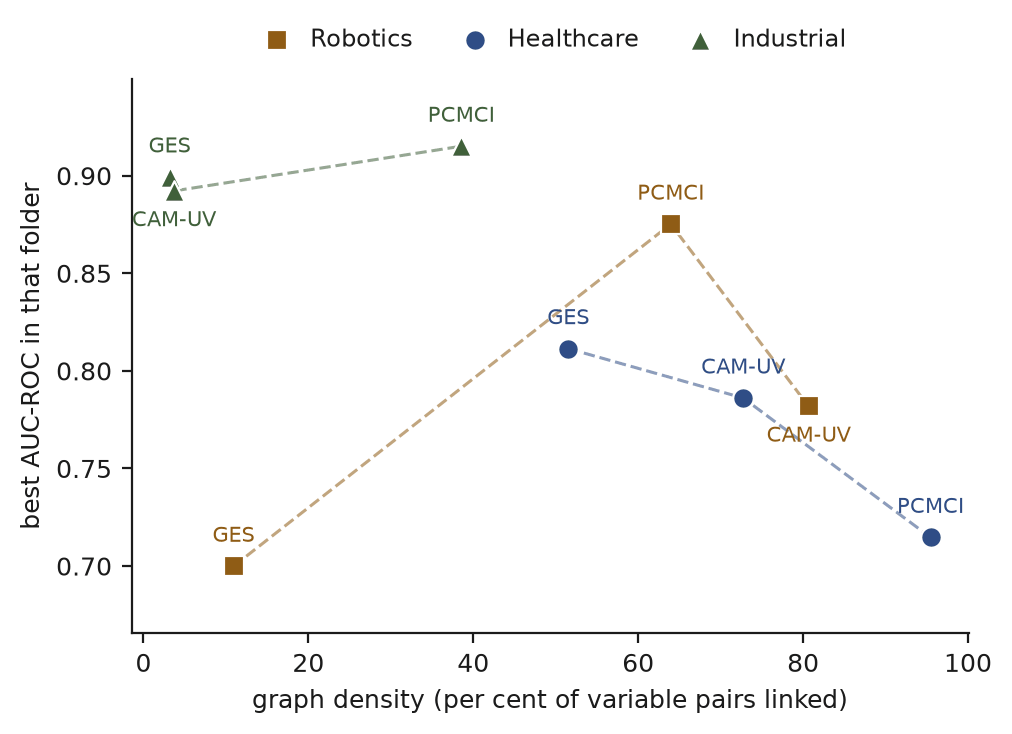
\includegraphics[width=0.82\textwidth]{fig_density_vs_auc.png}
  \caption[Graph density against detection performance]{Graph density against the best detection score obtained from that graph, for all nine algorithm--domain pairs. The healthcare series falls monotonically, which is the relationship Section~\ref{sec:density} argues from; the industrial series rises, which is why the mechanism is not offered as general; and robotics, where PCMCI works over 244 variables and the other two over 35, is confounded beyond interpretation.}
  \label{fig:density-auc}
\end{figure}

% GENERATED by Thesis/tools/make_tables.py -- do not edit by hand.
% Every figure below is read from a CSV written by the pipelines.
\begin{table}[htbp]
\centering
\small
\caption[Bite of the three-parent regression cap, for all nine algorithm--domain pairs]{Bite of the three-parent regression cap, for all nine algorithm--domain pairs. A target is regressed on at most three parents, chosen by shortest lag, so the design matrix is never wider than three columns plus an intercept. Targets are those variables the graph gives at least one parent. The final column is the share of discovered edges the cap discards, and it is what prevents graph density from acting through regression size: on robotics it removes 98.2\% of what PCMCI found and none of what GES found.}
\label{tab:parentcap}
\begin{tabular}{llrrrr}
\toprule
Domain & Algorithm & Targets & Edges & Capped & Edges dropped \\
\midrule
Robotics & PCMCI & 244 & 40808 & 100.0\% & 98.2\% \\
 & CAM-UV & 35 & 960 & 94.3\% & 89.5\% \\
 & GES & 32 & 65 & 0.0\% & 0.0\% \\
\midrule
Healthcare & PCMCI & 12 & 149 & 100.0\% & 75.8\% \\
 & CAM-UV & 12 & 87 & 83.3\% & 58.6\% \\
 & GES & 9 & 34 & 77.8\% & 26.5\% \\
\midrule
Industrial & PCMCI & 52 & 1108 & 100.0\% & 85.9\% \\
 & CAM-UV & 39 & 63 & 5.1\% & 4.8\% \\
 & GES & 25 & 42 & 4.0\% & 2.4\% \\
\bottomrule
\end{tabular}
\end{table}


\begin{figure}[htbp]
  \centering
  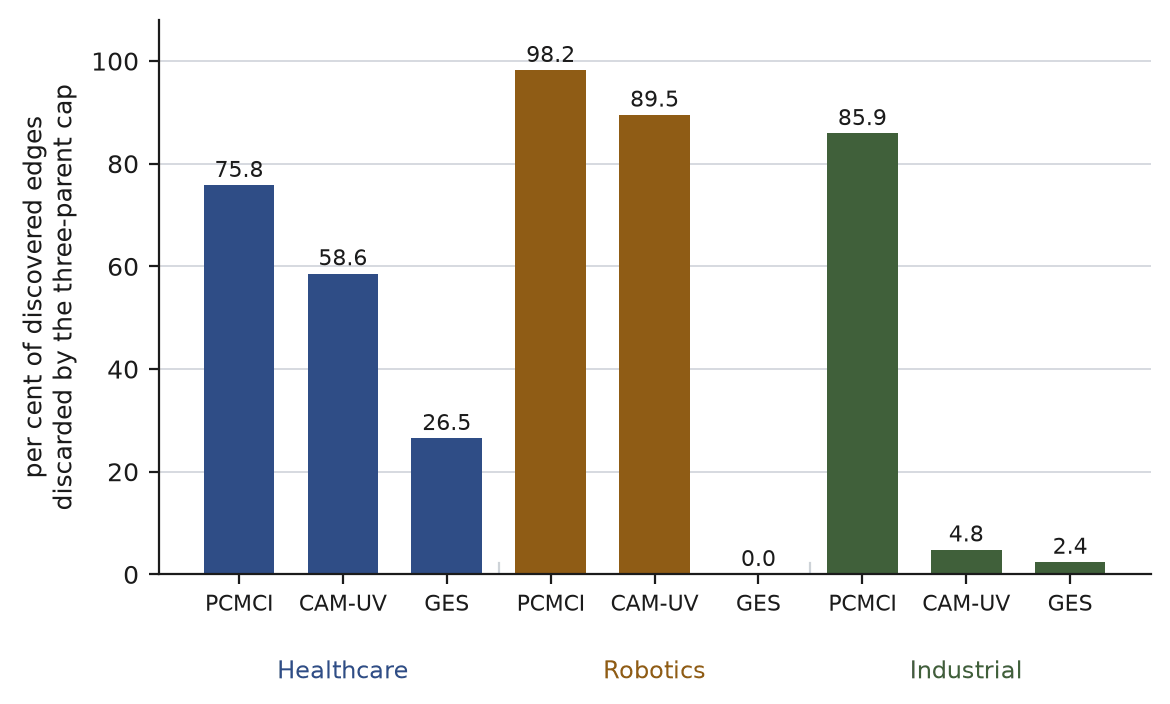
\includegraphics[width=0.86\textwidth]{fig_parent_cap.png}
  \caption[Share of each discovered graph discarded by the three-parent cap]{Share of each discovered graph discarded by the three-parent cap. The bars are the final column of Table~\ref{tab:parentcap}. What matters is that they are not equal: on robotics the cap removes 98.2\% of what PCMCI found and nothing at all of what GES found, so that comparison sets a whole graph against a small selection from another.}
  \label{fig:parentcap-bars}
\end{figure}

A component of that density moves with detection in the same way across these three domains, and it exists for one algorithm only. CAM-UV alone returns the set of variable pairs it assigns to an unobserved common cause, and the share of pairs in that set falls from domain to domain exactly as its detection score rises. Being specific to one algorithm it is reported in Appendix~\ref{app:confounders} rather than here, together with the synthetic ablation that fixes the sample size below which the method recovers nothing.

\section{The Eight-Lead Ablation}
\label{sec:eight-lead-ablation}

The eight-lead ablation quantifies how much of the causal pipeline's performance on the Healthcare dataset relied on algebraic redundancy. Removing the four leads governed by exact linear dependencies produces a sign flip across algorithm families. GES relies partially on this redundancy, its performance degrading across all three variants, with GES linear/ridge dropping from 0.8114 to 0.7418.

In the other direction, the redundant leads were actively harming specific PCMCI configurations. The PCMCI polynomial variant gains 0.1280, rising from 0.5075 to 0.6355, when the four dependent leads are removed. This is mechanically sound: evaluating a degree-three polynomial expansion over exact linear combinations introduces severe multicollinearity and degrades the conditioning of the regressions. Removing the redundant variables stabilises the model.

This ablation cannot be read directly as a within-algorithm test of the density mechanism, because comparing a twelve-variable density against an eight-variable one changes the denominator from 66 pairs to 28 and inflates the fraction even where absolute edge counts fall. Restricting the twelve-lead graph to the same eight leads removes that confound and permits the comparison over a common 28 pairs.

Under that restriction the algorithms separate, as Table~\ref{tab:lead_ablation} sets out. GES rises from 53.6 to 75.0\% density and loses 0.054 in mean AUC-ROC; CAM-UV rises from 78.6 to 100.0\% and loses 0.013. Both are consistent with the mechanism proposed in Section~\ref{sec:density}. PCMCI, by contrast, links 26 of 28 pairs under both conditions, an identical 92.9\%, while its mean AUC-ROC rises by 0.046. Its improvement therefore cannot be attributed to a change in graph density, and the multicollinearity account above is the remaining explanation.

% GENERATED by Thesis/tools/make_tables.py -- do not edit by hand.
% Every figure below is read from a CSV written by the pipelines.
\begin{table}[htbp]
\centering
\small
\caption[The eight-lead ablation over a common denominator]{The eight-lead ablation over a common denominator. Removing the four leads that are exact linear combinations of the others leaves 28 variable pairs; both density columns are counted over those same 28, so the twelve-lead figure is its graph restricted to the eight retained leads, not its own 66-pair density. Mean AUC-ROC is averaged over the three regression variants. GES and CAM-UV gain density and lose accuracy, as Section~\ref{sec:density} predicts; PCMCI links an identical 26 pairs under both conditions and gains, so its improvement cannot be a density effect and is attributed to relieved multicollinearity.}
\label{tab:lead_ablation}
\begin{tabular}{lcrrrrr}
\toprule
Algorithm & Linked 12/8 & Dens.\ 12 & Dens.\ 8 & AUC 12 $\uparrow$ & AUC 8 $\uparrow$ & $\Delta$ AUC $\uparrow$ \\
\midrule
PCMCI & 26 / 26 & 92.9\% & 92.9\% & 0.6134 & 0.6597 & \textbf{+0.0462} \\
GES & 15 / 21 & 53.6\% & 75.0\% & \textbf{0.7867} & 0.7325 & -0.0542 \\
CAM-UV & 22 / 28 & 78.6\% & 100.0\% & 0.7748 & \textbf{0.7620} & -0.0128 \\
\bottomrule
\end{tabular}
\end{table}


Two mechanisms are thus separable rather than confounded. Three algorithms remain too few to establish either, and the cross-algorithm caveats of Section~\ref{sec:density} continue to apply.

\section{Discovery Quality under Autocorrelation}
\label{sec:pcpcmci}

Section~\ref{sec:rw-cd} selects PCMCI as the constraint-based representative on the grounds that the standard method degrades under exactly the conditions these three domains present. Table~\ref{tab:pcpcmci} is that measurement. The series is synthetic and built to contain no cross-variable edges at all, so every link either algorithm reports is a false positive by construction and the false-positive rate is read directly off the output.

PC degrades as predicted. Its false-positive rate rises from 0.0429 at zero autocorrelation to 0.4982 at $\phi = 0.95$, a twelve-fold increase, so at the top of the sweep it links very nearly half of all variable pairs in a system that contains no links. PCMCI does not degrade: its rate is flat across the whole sweep, moving from 0.2946 to 0.2839 as $\phi$ rises. Flatness in $\phi$, rather than any particular level, is the property the algorithm selection rests on, and it is what PC lacks.

The level does require a qualification that the last two columns make visible. Applying the false-discovery correction holds PCMCI between 0.0500 and 0.0589 across the sweep; without it the rate sits near 0.28. This pipeline leaves that correction off, so the uncorrected column is the one describing the configuration evaluated throughout this thesis. The graphs reported in Section~\ref{sec:density} are therefore produced by a variant whose false-positive rate on a null system is roughly 0.28 instead of 0.05, which is consistent with the dense healthcare graph reported there and is a further reason to read that density as over-linking and not as recovered structure.

% GENERATED by Thesis/tools/make_tables.py -- do not edit by hand.
% Every figure below is read from a CSV written by the pipelines.
\begin{table}[htbp]
\centering
\caption[False-positive rate of PC against PCMCI on synthetic data built to contain no cross-variable edges]{False-positive rate of PC against PCMCI on synthetic data built to contain no cross-variable edges, so every reported link is a false positive by construction. The sweep varies the autocorrelation coefficient $\phi$ over 8 variables and 1000 samples, averaged over 20 seeds at $\alpha = 0.05$. PC degrades sharply; PCMCI does not degrade at all, which is why it is the constraint-based representative here. The last two columns are the same algorithm with and without the false-discovery correction: the pipeline runs the uncorrected variant, so that column describes the configuration evaluated in this thesis and the corrected one does not.}
\label{tab:pcpcmci}
\begin{tabular}{lrrr}
\toprule
$\phi$ & PC $\downarrow$ & PCMCI, as run $\downarrow$ & PCMCI, FDR $\downarrow$ \\
\midrule
0.00 & 0.0429 & 0.2946 & 0.0500 \\
0.30 & 0.0518 & 0.2804 & 0.0589 \\
0.50 & 0.1393 & 0.2714 & 0.0589 \\
0.70 & 0.2393 & 0.2768 & 0.0554 \\
0.90 & 0.4321 & 0.2839 & 0.0500 \\
0.95 & 0.4982 & 0.2839 & 0.0536 \\
\bottomrule
\end{tabular}
\end{table}


\section{Computational Cost}
\label{sec:runtime}

Cost is reported here because a structural front-end is only useful if it can be afforded, and because the measurement existed and had gone unreported. Table~\ref{tab:runtime} gives wall-clock detection time for all 27 configurations. Discovery is cached and excluded, so these figures describe the recurring cost rather than the one-off cost of learning a graph.

The table does not rank the three algorithms, and the variable and subsample columns are printed so that a reader can see why not. PCMCI works over 244 variables on robotics where the other two work over 35, and over every industrial sample where they take one in ten. No domain presents the three with the same workload, so the figures bound what each configuration cost as it was run and support no comparison across algorithms. This is the same confound recorded for graph density in Section~\ref{sec:density}, and it has the same origin.

A second limit belongs in the same breath, because it is the more consequential of the two. Discovery is the step at which these algorithms differ by orders of magnitude, and it is not measured here at all. It is paid once per algorithm and dataset and then cached, so it does not recur per regression variant; re-running it to time it would rebuild CAM-UV's graph, which is not reproducible between runs, and would therefore change every result in this dissertation. The measurement was not worth that price. What Table~\ref{tab:runtime} reports is consequently the recurring operational cost of a deployed detector and not the total cost of adopting a method.

One comparison is available, because it holds workload fixed. Within each of the nine algorithm--domain cells the three regression variants see an identical variable set at an identical subsampling rate, and in all nine the RBF variant is the slowest, by between 1.6 seconds on GES industrial and 23.6 on PCMCI industrial. The difference between linear and polynomial never exceeds 4.4 seconds by comparison, and changes sign in two of the nine cells with a third tied, so it is not a consistent effect at all. What detection time is sensitive to is the random Fourier feature map, rather than the polynomial expansion.

The absolute magnitudes bound the practical claim. The slowest configuration in the grid is PCMCI industrial with the RBF map at 151.5 seconds, and the whole grid runs in under three minutes per configuration, on a 15~W mobile processor, which is the weaker end of the hardware a practitioner would deploy on instead of the stronger. At these problem scales cost does not separate the methods, and the choice between them should be made on the accuracy and attribution grounds argued above. Whether that survives at larger variable counts is not established here, and the limit that was encountered is an algorithm's rather than the grid's. The 244-variable PCMCI runs are the largest measured, while Section~\ref{sec:disc-threats} records that a 160-variable GES run did not converge in 66 minutes of CPU. That asymmetry is why GES and CAM-UV take robotics at 35 variables, and therefore why this table contains no cell in which all three algorithms meet on the same workload.

% GENERATED by Thesis/tools/make_tables.py -- do not edit by hand.
% Every figure below is read from a CSV written by the pipelines.
\begin{table}[htbp]
\centering
\small
\caption[Wall-clock detection time for all 27 configurations, in seconds]{Wall-clock detection time for all 27 configurations, in seconds. All 27 were measured in one session on the machine that produced every result in this dissertation: an Intel Core i5-8250U at 1.60~GHz, four cores and eight threads, with 32~GB of memory, under Windows 11. That is a 15~W mobile processor and not a workstation, which is worth knowing in both directions: it makes the modest absolute cost reported here a stronger claim, and it is the machine on which the 160-variable GES run failed to converge. The timing harness refuses to start under CPU contention, so no other work distorted these figures; they remain specific to that machine and only the relative magnitudes travel. Discovery is cached and excluded; these are the detection runs. The variable and subsample columns are given because they prevent the table from being read as a ranking: on robotics PCMCI works over 244 variables where the other two work over 35, and on industrial it uses every sample where they take one in ten. No domain presents the three algorithms with the same workload, so the figures bound the cost of each configuration as it was run and support no comparison between algorithms.}
\label{tab:runtime}
\begin{tabular}{lllrrr}
\toprule
Algorithm & Domain & Variant & Vars & Subs. & Seconds $\downarrow$ \\
\midrule
PCMCI & Robotics & Linear / Ridge & 244 & 74 & 44.0 \\
 & Robotics & Polynomial degree 3 & 244 & 74 & 46.4 \\
 & Robotics & RBF + Ridge & 244 & 74 & 50.8 \\
 & Healthcare & Linear / Ridge & 12 & 7 & 18.9 \\
 & Healthcare & Polynomial degree 3 & 12 & 7 & 19.5 \\
 & Healthcare & RBF + Ridge & 12 & 7 & 22.5 \\
 & Industrial & Linear / Ridge & 52 & 1 & 132.3 \\
 & Industrial & Polynomial degree 3 & 52 & 1 & 127.9 \\
 & Industrial & RBF + Ridge & 52 & 1 & 151.5 \\
\midrule
GES & Robotics & Linear / Ridge & 35 & 10 & 20.7 \\
 & Robotics & Polynomial degree 3 & 35 & 10 & 20.7 \\
 & Robotics & RBF + Ridge & 35 & 10 & 35.9 \\
 & Healthcare & Linear / Ridge & 12 & 10 & 18.2 \\
 & Healthcare & Polynomial degree 3 & 12 & 10 & 18.4 \\
 & Healthcare & RBF + Ridge & 12 & 10 & 27.7 \\
 & Industrial & Linear / Ridge & 52 & 10 & 13.5 \\
 & Industrial & Polynomial degree 3 & 52 & 10 & 13.7 \\
 & Industrial & RBF + Ridge & 52 & 10 & 15.1 \\
\midrule
CAM-UV & Robotics & Linear / Ridge & 35 & 10 & 22.1 \\
 & Robotics & Polynomial degree 3 & 35 & 10 & 23.0 \\
 & Robotics & RBF + Ridge & 35 & 10 & 38.6 \\
 & Healthcare & Linear / Ridge & 12 & 10 & 21.4 \\
 & Healthcare & Polynomial degree 3 & 12 & 10 & 22.2 \\
 & Healthcare & RBF + Ridge & 12 & 10 & 35.1 \\
 & Industrial & Linear / Ridge & 52 & 10 & 16.2 \\
 & Industrial & Polynomial degree 3 & 52 & 10 & 16.0 \\
 & Industrial & RBF + Ridge & 52 & 10 & 18.9 \\
\bottomrule
\end{tabular}
\end{table}


%=======================================================================
%  CHAPTER 7 -- DISCUSSION
%=======================================================================
\chapter{Discussion}
\label{ch:discussion}

%-----------------------------------------------------------------------
\section{When Causal Structure Pays}
\label{sec:disc-when}

The central argument of this thesis is that causal anomaly detection is not universally superior to standard machine learning; its advantage is conditional on the character of the domain. Where an anomaly manifests as a large excursion in signal amplitude, a causal graph is unnecessary: a statistical threshold or a reconstruction autoencoder captures the deviation perfectly well. Where the anomaly is relational, with the variables remaining within their nominal ranges while the relationship between them breaks, structure becomes the deciding factor.

The conditional advantage can be quantified rather than argued, using the parameter-free trivial control as the instrument. Its AUC-ROC measures how much of a domain's fault signature is pure amplitude. Set against the best causal configuration and the best tuned neural baseline in each domain, the relationship is monotone, as Table~\ref{tab:causal-advantage} and Figure~\ref{fig:conditional} show.

\begin{figure}[htbp]
  \centering
  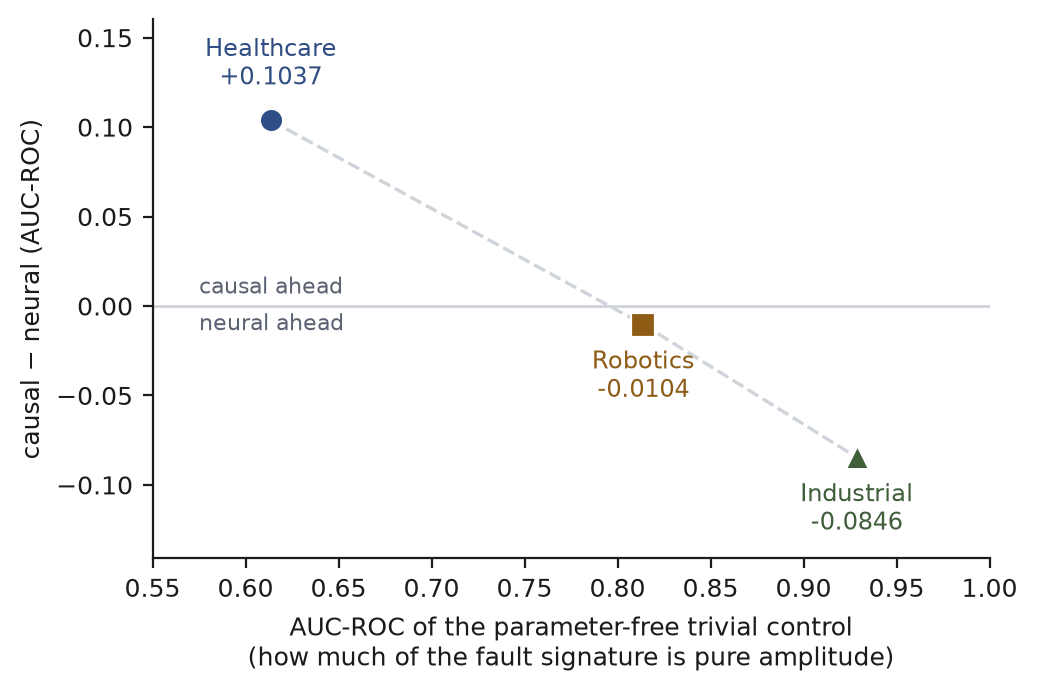
\includegraphics[width=0.78\textwidth]{fig_conditional_advantage.png}
  \caption[The causal advantage against the trivial control's score]{The causal advantage against the trivial control's score. The horizontal axis is the parameter-free control's AUC-ROC, which indexes how much of a domain's fault signature is pure amplitude; the vertical axis is the margin of the best causal configuration over the best tuned neural baseline. The connecting line is drawn to make the ordering readable and is not a fit: three points cannot establish a trend, and the experiment that would test one is stated at the end of this section.}
  \label{fig:conditional}
\end{figure}

\begin{table}[htbp]
\centering
\caption[The causal advantage shrinks monotonically as the trivial control's score rises]{The causal advantage shrinks monotonically as the trivial control's score rises. All four columns are AUC-ROC, so higher is better throughout. The neural column is the best of the three tuned architectures in each domain: LSTM on Healthcare, TCN on Robotics and Industrial. Only the Healthcare row carries a bold cell, because it is the only one whose ordering survives the bootstrap intervals: on Robotics and on Industrial the neural score falls inside the causal configuration's interval, so the leading point estimate there is not a winner and is not marked as one.}
\label{tab:causal-advantage}
\begin{tabular}{lrrrr}
\toprule
Domain & Trivial $\uparrow$ & Causal $\uparrow$ & Neural $\uparrow$ & Causal $-$ Neural $\uparrow$ \\
\midrule
Healthcare & 0.6136 & \textbf{0.8114} & 0.7077 & $\mathbf{+0.1037}$ \\
Robotics   & 0.8139 & 0.8752 & 0.8856 & $-0.0104$ \\
Industrial & 0.9286 & 0.9151 & 0.9997 & $-0.0846$ \\
\bottomrule
\end{tabular}
\end{table}

On Healthcare the faults are overwhelmingly relational, the trivial control reaching only 0.6136, and the causal pipeline decisively outperforms the best neural architecture. On Robotics the fault character is mixed at 0.8139, and although the causal point estimate of 0.8752 trails the neural baseline at 0.8856, the two are not separable: the neural score falls well inside the causal configuration's bootstrap interval of $[0.7559, 0.9587]$. On Industrial the faults are heavily amplitude-driven at 0.9286, and the causal pipeline trails not only the neural baselines but the trivial control itself, 0.9151 against 0.9286, a method with no learned parameters at all. The interval test applied to Robotics a moment ago must be applied here too, and it cuts the same way: 0.9286 falls inside the causal configuration's bootstrap interval of $[0.8880, 0.9394]$, so this ordering is no more separable than that one. What the evidence supports on Industrial is the absence of a causal advantage, not a decisive victory for the control. The argument of this section needs only the weaker claim: a structural method that cannot be distinguished from a parameter-free threshold has not earned its cost, whether or not it is strictly beaten by it.

The mechanism proposed for the Healthcare result is the sparse structural constraint. It has to be stated precisely, because the three-parent cap already restricts every regression to a small parent set whatever graph produced it, so smallness alone cannot be what separates the algorithms. What separates them is whether the discovery step chooses those parents or merely supplies a pool from which a lag-ordered tiebreak chooses them: GES offers 3.78 candidates per lead and the cap barely binds, while PCMCI offers 12.42 and the cap discards three quarters of them. On that reading the sparse graph limits fitting to superficial variance because it, not an arbitrary rule, determines what the regression sees. As established in Section~\ref{sec:density}, however, that evidence supports the mechanism on Healthcare alone. Density there is confounded with discovery sample size, and the relationship between sparsity and performance reverses outright on Industrial. The mechanism is offered as the best available explanation of one domain, not as a general law.

The falsifiable form of the claim is therefore this: the advantage of a structural causal detector over a magnitude-based detector shrinks as the trivial control's AUC-ROC rises. All three domains evaluated here are consistent with it, and three points do not establish a trend. A genuine test would require twenty or thirty domains, plotting the causal advantage against the trivial score. The barrier is not effort but data: each domain requires continuous multivariate observations with a verified fault-free period and faults whose ground truth is known, and that combination remains rare among public benchmarks. Stating the test that would refute the hypothesis, and why it cannot yet be run, is more useful than asserting the hypothesis on three points.

\section{Why the Algorithm Ranking Is Unstable}
\label{sec:disc-ranking}

Where the top two configurations in a domain share an algorithm they also share an evaluation sample set, and DeLong's test separates them: GES linear from GES polynomial on Healthcare at $p = 0.001119$, and PCMCI with RBF features from PCMCI polynomial on Robotics at $p = 0.000077$. What cannot be tested is the comparison this section is actually about. On Industrial the runner-up belongs to a different algorithm, and because PCMCI subsamples at a different rate from GES the two do not score the same observations, so no paired test exists. The regression-variant ranking within an algorithm is therefore established; the algorithm ranking across a domain is not. What follows is an interpretation of an empirical ordering, not an explanation of a demonstrated one.

PCMCI takes the highest score on Industrial. Through the ParCorr test it assumes linear relations while handling autocorrelation natively, by conditioning on past states and not treating observations as independent. That assumption matches the continuous, strongly autocorrelated fluid and thermal dynamics of the Tennessee Eastman Process.

GES takes the highest score on Healthcare. Because it scores an equivalence class and does not privilege temporal order, it suits data in which an electrical event registers across several leads at once. The explanation carries a caveat that cannot be omitted. The eight-lead ablation reduced GES from 0.8114 to 0.7418 when the algebraically dependent leads were removed. GES is well suited to recovering exact, instantaneous linear identities, and that is precisely the difficulty: a substantial part of the structure it exploited was Einthoven's algebra rather than cardiac physiology. The algorithm was doing what it is good at, on relations that were arithmetic, not biological.

PCMCI's own graph on this domain points the same way, and here the lag is genuinely discovered, not a pipeline convention: as Section~\ref{sec:setup-lag} reports, every parent PCMCI's Healthcare regressions retain after the three-parent cap is contemporaneous rather than lagged. That is consistent with the same physiology, since a limb-lead identity holds between simultaneous voltages and not ones separated in time. It is also why a search free to place a parent at any lag from zero to three places it at zero almost without exception on this domain specifically.

CAM-UV never takes the highest score in any domain, and its two failure modes are quantified and not supposed. Table~\ref{tab:confounder} in Appendix~\ref{app:confounders} reports both across the three domains. On Robotics it saturates: 80.7\% of all variable pairs are assigned to the latent confounder set, leaving no observed-parent edges at all, so the structural constraint that is supposed to do the work is absent. On Industrial it starves, with 0.67 samples per variable, far below the 200-sample floor at which the confounder ablation found recovery never to succeed under any significance level.

\section{Structure Recovery Versus Detection Performance}
\label{sec:disc-structure}

The methodological takeaway of this evaluation is that downstream detection performance cannot validate an upstream causal graph. A high AUC-ROC does not imply the discovered structure is physically accurate, and a structurally flawed graph does not preclude competitive detection. Three pieces of evidence establish the disconnect.

First, density can actively degrade discrimination. On Healthcare, PCMCI constructs a saturated graph at 95.5\% density and achieves the lowest causal score in the domain, 0.7147. GES constructs a far sparser graph at 51.5\% and takes the highest, 0.8114. A denser capture of statistical dependency harmed the detector rather than helping it.

Second, a structurally empty graph can still detect competitively. On Robotics, CAM-UV produces a graph 80.7\% saturated with latent confounder pairs and containing no observed-parent edges whatsoever. Despite that, its best variant reaches 0.7818, above every GES configuration in the domain, which range from 0.5906 to 0.6999. A graph carrying no observed structure at all detected faults better than a formally sparse one.

Third, and most consequentially, attribution can succeed on a graph that lacks the relevant structure entirely. During the \texttt{LedsControl} attack the variable the documented requirement names, \texttt{TabletTouchX}, sits at rank 78 of 249 by standardised deviation: it is emphatically not the sensor that moved most. The causal attribution ranks it first in 9 of 9 configurations, and it does so including in the six configurations whose graphs exclude every LED channel, so no LED-to-tablet relation can be represented in them at all. The attribution succeeds despite the graph missing the structure that would appear to explain it.

The conclusion is uncomfortable but hard to avoid: a pipeline reporting only an AUC-ROC provides no evidence that its discovered structure is physically meaningful. The claim can be put in testable form. Two graphs built on incompatible structural premises can produce detection scores that are indistinguishable. On Industrial, a CAM-UV graph whose sparsity is an artefact of 35 samples for 52 variables scores 0.8922 against 0.8994 for a GES graph at 3.2\% density, so the metric has no power to discriminate between them. The anomaly score measures the capacity of the regression filter downstream of the graph; it does not validate the discovery upstream of it.

\section{Explainability Without Ground-Truth Attribution}
\label{sec:disc-xai}

The claim of this section is that the causal pipeline changes what attribution reports. It names the variable whose modelled relationship broke instead of the one that moved furthest.

The evaluation has something uncommon in explainability research: a ground truth. Because the dataset documents which subsystem each injected attack targets, the attributions can be scored against a known answer rather than against a human judgement of plausibility. Most attribution evaluation lacks this and is reduced to asking whether an explanation looks reasonable.

Against that ground truth the causal attribution names the correct subsystem in 9 of 9 configurations for \texttt{LedsControl}, returning \texttt{TabletTouchX}, and in 8 of 9 for \texttt{JointControl}, returning \texttt{KneePicthTemp}. Neither is the sensor that moved most. During \texttt{LedsControl} the tablet channel sits at rank 78 of 249 by standardised deviation, far below the LED channels themselves; during \texttt{JointControl} the knee temperature sits at rank 4, below \texttt{RShoulderPitch} at rank 1. A detector ranking by magnitude would return neither. The post-hoc SHAP attribution over the neural baselines, by contrast, satisfies the LED requirement in 2 of 3 architectures and the joint requirement in none, all three naming \texttt{RShoulderPitch}, which is precisely the variable that moved most.

The most valuable result here is not the 9 of 9 but the 8 of 9. The single failure, PCMCI with polynomial features returning \texttt{WheelBStiff}, establishes that the check is capable of failing. A test that always passes distinguishes nothing, and without that miss the seventeen successes would be indistinguishable from a metric that returns the target by construction. The failure is what makes the rest evidence.

Two qualifications keep the comparison honest. The first is that it is structural, not like-for-like: the causal attribution reads coefficient drift from a recursive least squares filter while the neural attribution computes SHAP values over a reconstruction error, so what is compared is two pipelines instead of two attribution methods applied to a common model. The second is narrower and sharper. As established in Section~\ref{sec:method-attribution}, the \texttt{JointControl} result depends on the raw $L_2$ ranking retained for parity with the reference implementation. Under the baseline-normalised rule used in the other two domains the same data returns \texttt{LedEarR3} and \texttt{LedEarL3}, and the result would have been a failure. The attribution is therefore correct under the metric this domain uses, and the metric is not neutral.

A third qualification is the most important, because the two faults discussed
here are the two on which the causal attribution looks strongest, and they are
two of the forty-three anomaly classes this work scores, and two of the
twenty-two that carry a documented cause to score against. Section~\ref{sec:attribution}
repeats the comparison across all of them in the three domains, against the
documented cause of each, and the ordering does not survive: post-hoc attribution
over the neural baselines is nowhere less relevant than the intrinsic causal
attribution, once the comparison is restricted to methods ranking pools of the
same size. That restriction is not a convenience: GES ranks nine of the twelve
leads and CAM-UV 35 of the 244 robot sensors, so a raw percentage difference
against either mixes a smaller search space into what looks like a method
difference. How much of any of this is demonstrated rather than merely observed
is settled in Section~\ref{sec:attr-intervals}, and the answer is one comparison
of the nine made at that depth. The robot's three attack classes and the
plant's five documented actuators cannot reach the 5\% level whatever the numbers
are, so neither domain decides anything; on the electrocardiogram, where fourteen
classes do support a test, the only separation at the depth this thesis reports
attribution at is SHAP over PCMCI, and it survives correction for the three
comparisons made within that domain. The LED and joint
results above are real, they are the cases the documented requirement was written
around, and they are not representative. What the causal side retains at the scale
of the full evaluation is narrower and is stated there: on the electrocardiogram
its configurations agree with one another about the specific record in front of
them, where the neural architectures return something close to a fixed ranking of
the leads.

\section{Threats to Validity}
\label{sec:disc-threats}

\begin{table}[htbp]
\centering
\small
\setlength{\tabcolsep}{4pt}
\caption{Threats to validity, their severity and what bounds them.}
\label{tab:threats}
\begin{tabularx}{\textwidth}{@{}p{0.31\textwidth} l X@{}}
\toprule
Threat & Severity & Mitigation \\
\midrule
Scoring resolution differs by algorithm & High & Bounded by ablation; equalising is infeasible in one direction \\
Ridge penalty varies by variant on Robotics & Moderate & Identical across algorithms in every cell, so RQ1 is unaffected \\
One run per causal configuration; CAM-UV not reproducible & Moderate & Bootstrap intervals over real per-sample scores; three seeds for the neural baselines \\
One dataset per domain & Moderate & Stated; the strongest result depends on an unusually favourable structure \\
Injected rather than naturally occurring faults & Moderate & Ground truth is available in exchange, which is what permits the attribution evaluation \\
Prevalence varies from 0.5717 to 0.9524 & Low & AUC-ROC is prevalence-independent and is used as the primary metric \\
\bottomrule
\end{tabularx}
\end{table}

Table~\ref{tab:threats} summarises the threats, their severity and what bounds each; the subsections below take the most consequential in turn.

\subsection{Internal validity}

The most severe threat is the scoring resolution mismatch, and it is stated first because an examiner meets it immediately. PCMCI subsamples at 74, 7 and 1 across the three domains where GES and CAM-UV are fixed at 10, so within a domain the three algorithms do not score the same series. Two ablations bound the effect without removing it: forcing PCMCI on Robotics to rate 10 drops it from 0.8752 to 0.6813, and forcing GES on Healthcare to rate 1 drops it from 0.8114 to 0.6184. Equalising the rate is not available in one direction, since a 160-variable GES run did not converge in 66 minutes of CPU. The consequence for interpretation is stated plainly: RQ1 compares each algorithm as it is intended to be applied, preprocessing included, and does not isolate the discovery step.

The second is the ridge penalty, which varies by regression variant on Robotics to keep the polynomial and random-feature design matrices numerically conditioned. It is fully mitigated for RQ1, since the penalty is identical across all three algorithms within every cell, and partially confounds RQ2 on that domain alone.

The third is reproducibility. Each causal configuration was run once, and CAM-UV is not exactly reproducible between runs. The mitigation is that uncertainty is quantified from the real per-sample scores through a moving-block bootstrap instead of from repeated runs, and the neural baselines are averaged over three seeds.

\subsection{External validity}

Three domains with one dataset each is a narrow base, but the sharper threat concerns the strongest result specifically. The Healthcare advantage depends on the twelve ECG leads satisfying exact algebraic identities, and the eight-lead ablation shows how much of it that structure supplied. Exact linear relations among observed variables are a favourable case that will not generally be present in noisy field data, so the result should not be read as a general claim about biological signals.

\subsection{Construct validity}

The robotics faults are injected, and the industrial faults are simulated. The healthcare classes are not: each one is a real recorded ECG carrying a clinician-assigned diagnosis. That is a genuine limitation, and it purchases the ground truth without which the attribution evaluation in Section~\ref{sec:disc-xai} would not be possible at all. The 95th-percentile threshold is a design choice and not a derived optimum; it is defensible because it is applied identically everywhere and never consults an anomaly label, not because 95 is correct. And AUC-PR is not comparable across domains, since prevalence ranges from 0.5717 on Healthcare to 0.9524 on Industrial; AUC-ROC is prevalence-independent and is used as the primary metric throughout for that reason.

\subsection{Statistical conclusion validity}

Two of the 27 configurations cannot be distinguished from chance. GES with linear features on Robotics reaches 0.5906 with an interval of $[0.4873, 0.6761]$, and PCMCI with polynomial features on Healthcare reaches 0.5075 with an interval of $[0.4429, 0.5663]$, the latter sitting almost exactly on chance, not merely overlapping it. Beyond this, and as established in Section~\ref{sec:disc-ranking}, cross-algorithm comparisons admit no paired test, because the subsample policy means PCMCI does not score the same observations as GES or CAM-UV. With a single run per cell there is also no within-cell variance, so no formal test of the algorithm-by-regression interaction is available.

%=======================================================================
%  CHAPTER 8 -- CONCLUSION
%=======================================================================
\chapter{Conclusion and Future Work}
\label{ch:conclusion}

\section{Summary of the Work}
\label{sec:conc-summary}

This thesis constructed and evaluated a uniform causal anomaly detection pipeline to determine whether, and more usefully when, causal structure provides a measurable advantage over standard machine learning. The evaluation was executed as a combinatorial grid: three causal discovery algorithms (PCMCI, GES, CAM-UV) crossed with three regression families (linear, polynomial, RBF) across three domains (Robotics, Healthcare, Industrial). So that differences would be attributable to the algorithms, not to tuning, the scoring mechanism, the thresholding rule and the attribution depth were held constant, enforced programmatically by an automated audit on every build.

\section{Answers to the Research Questions}
\label{sec:conc-rqs}

\subsection*{RQ1 --- Algorithm effectiveness and ranking stability}
There is no universally optimal causal algorithm. PCMCI takes the highest score on Robotics (0.8752) and Industrial (0.9151), while GES takes the highest on Healthcare (0.8114). The regression-variant ranking within an algorithm is statistically established: GES linear separates from GES polynomial on Healthcare at $p = 0.001119$, but the cross-algorithm ranking within a domain is not testable at all, because the subsampling policy means the algorithms do not score the same observations. The domain ordering is empirical; the algorithmic ranking is not established.

\subsection*{RQ2 --- Interaction between discovery and regression}
The regression family interacts with both the discovery algorithm and the domain. Across the nine algorithm--domain cells the RBF variant takes five, linear two and polynomial two, and GES prefers a different variant in each of the three domains. Neither axis dominates: which regression family is best cannot be stated without naming both the algorithm and the domain.

\subsection*{RQ3 --- Causal versus non-causal detection}
The advantage is conditional on the character of the faults. Causal methods outperform the best tuned neural baseline on Healthcare, 0.8114 against 0.7077. On Industrial the causal pipeline is beaten by the neural baselines and cannot be separated from the parameter-free trivial control, 0.9151 against 0.9286, which lies inside its bootstrap interval. On Robotics the two are not separable.

\subsection*{RQ4 --- Attribution quality}
The causal pipeline names the variable whose modelled relationship broke instead of the one that deviated most. It returns \texttt{TabletTouchX} in 9 of 9 Robotics configurations for the LED attack and \texttt{KneePicthTemp} in 8 of 9 for the joint attack, and neither is the variable that moved most: the tablet channel ranks 78th of 249 by standardised deviation and the knee temperature 4th.

The more striking half of this result is that the attribution does not require the graph to contain the relation that would explain it. Six of the nine LED configurations return the correct variable from graphs holding no LED channel whatsoever, the variance-ranked cap applied by GES and CAM-UV on Robotics having excluded every one. PCMCI, which applies no cap and sees all 244 variables, returns the same answer. A correct explanation was produced from a structure that does not contain the explanation.

Those are two faults of the forty-three this work scores, and the answer does not hold at that scale. Scored against the documented cause of each of the twenty-two anomaly classes that carry one, across all three domains, the intrinsic attribution is no more relevant than post-hoc attribution over the neural baselines. Paired over classes, only the electrocardiogram carries enough scorable classes to decide the question, and there the intrinsic attribution is measurably behind under PCMCI and indistinguishable from post-hoc attribution under GES and CAM-UV. So the answer to RQ4 is yes on the question as asked, since the attribution does name the variable whose relationship broke and not the one that moved most, and no on the question a reader will ask next, since in the four comparisons where both sides rank a pool of the same size the causal pipeline never names it correctly more often than the post-hoc one. What it does retain is set out in Section~\ref{sec:attribution} and returned to in the closing remarks.

\subsection*{Why CAM-UV places as it does}
This is not one of the four questions, but it is what explains the answer to the first of them. CAM-UV never takes the highest score in any domain, and its latent confounder mechanism shows three distinct regimes that account for it. On Robotics it saturates, assigning 80.7\% of all variable pairs to the latent set and leaving no observed-parent edges at all, so the structural constraint that is supposed to do the work is absent. On Industrial it starves, with 0.67 samples per variable leaving the independence test no power to flag anything. Healthcare falls between them, saturating at 59.1\% and reaching 0.7861. The synthetic ablation confirms the reading without excusing it: recovery of a planted confounder is monotone in sample size, never succeeding at 200 and succeeding at every significance level tested by 1500.

\section{Contributions Revisited}
\label{sec:conc-contributions}

Section~\ref{sec:contributions} claimed three, and each is revisited here against what the evaluation actually delivered rather than what it set out to.

C1, the systematic evaluation, holds. The 27 configurations differ only along the two
declared methodological axes, across domains of 244, 52 and 12 variables, and Section~\ref{sec:method-overview} describes the audit that enforces this on every build rather than asserting it. The linearity assumption was relaxed in turn and not left in place, and the answer to RQ2 is that no regression family dominates: which one performs best cannot be stated without naming both the algorithm and the domain.

C2, the accuracy against explainability tradeoff, holds in a more interesting form than it was claimed. The detection half is conditional and the condition is measurable in advance, which is the finding this work would be cited for: the advantage of causal structure over the best tuned neural baseline shrinks monotonically as the score of a parameter-free control rises, so a question usually settled by building both methods can be estimated before either is built. The explainability half does not track it. Attribution succeeds in 9 of 9 configurations for the LED fault, six of those from graphs containing no LED channel at all, and in 8 of 9 for the joint fault, including on domains where the detection advantage has gone. The two halves of the tradeoff therefore come apart, and a practitioner choosing on detection alone would discard the explanatory capability for nothing. That capability is not a higher score: scored across the twenty-two anomaly classes that carry a documented cause, and over pools of matched size, the intrinsic attribution is no more relevant than the post-hoc one, and what it offers instead is a named broken relationship and, on the electrocardiogram, agreement that is specific to the record being explained. One qualification is recorded in Section~\ref{sec:disc-xai}: the joint-fault half depends on the ranking metric this domain uses and would have read as a failure under the other.

C3, the comparison against neural architectures, holds on both axes it was claimed on. On detection the three tuned autoencoders and the parameter-free control were evaluated under the identical label-blind rule, and the ordering between families changes with the domain and is not fixed. On explanation, post-hoc SHAP over those baselines returned the variable that moved furthest for the joint fault, naming RShoulderPitch, the single largest raw deviation in the system, in all three architectures, where the causal attribution named the thermal cause ranked fourth. That single fault is the clearest case for the distinction the comparison exists to draw, and it does not generalise. Scored against the documented cause of each of the twenty-two anomaly classes that carry one, and restricted to the comparisons in which both sides rank a pool of the same size, the post-hoc attribution is nowhere less relevant than the intrinsic one. The contribution therefore holds as a comparison rather than as a demonstration of causal superiority.

Two further findings emerged instead of being sought, and neither was claimed as a contribution. Downstream detection performance cannot validate an upstream causal graph: a structurally empty graph produced competitive detection, and two graphs built on incompatible premises produced indistinguishable scores, so a pipeline reporting only an AUC-ROC offers no evidence that its recovered structure is physically meaningful. And treating the subsampling rate as a property of each algorithm forecloses cross-algorithm significance testing, quantified in Table~\ref{tab:delong-summary}: 54 of the 108 within-domain comparisons admit no paired test, split identically 18 against 18 in every domain, and every unpairable one involves PCMCI. The empirical bounding of CAM-UV on real data, with its measured saturation and starvation regimes and the sample-size floor below which recovery of a planted confounder never succeeded, is reported in Appendix~\ref{app:confounders} and not carried here.

\section{Relation to Prior Work}
\label{sec:disc-prior}

This thesis does not establish that causal anomaly detection outperforms or underperforms deep learning in general, and no such claim is made. What it establishes is narrower and, for a reader deciding how to evaluate a method, more useful: that the comparison as conventionally constructed omits the control that determines how its result should be read.

The Industrial domain demonstrates this directly. Reported in the standard form, best causal configuration against best tuned neural baseline, the result is 0.9151 against 0.9997, and the conclusion available from those two numbers is that causal methods underperform on industrial process data. Adding a parameter-free control changes the conclusion rather than qualifying it. The trivial mean absolute $z$-score reaches 0.9286, above the causal pipeline and requiring no learned parameters whatsoever. The finding is therefore not that the causal method failed but that neither method's structure did work a threshold could not: the faults are amplitude excursions, and there is little relational signal for either to exploit. Those are different conclusions with different consequences for a practitioner, and only the second is supported once the control is present.

This is consistent with three separate critiques of evaluation practice, which are worth keeping distinct because they identify different faults. Wu and Keogh~\cite{wu2023flawed} argue that the benchmarks themselves manufacture an appearance of progress. Schmidl et al.~\cite{schmidl2022anomaly}, re-implementing 71 algorithms across 976 datasets, report no clear winner between algorithm families. Kim et al.~\cite{kim2022rigorous} show that the point-adjustment protocol inflates scores to the point where a random score looks competitive. None of the three establishes that elaborate detectors lose to trivial baselines as a general rule; what they establish jointly is that the protocol, not the architecture, frequently decides the reported ordering. The contribution here is to demonstrate, on one domain, that causal pipelines are not exempt from that finding, a possibility the causal discovery literature has had little occasion to test, since parameter-free controls are rarely reported alongside them.

A second point concerns attribution. Evaluation of explanations frequently rests on whether an explanation appears reasonable to a reader, a practice criticised by Doshi-Velez and Kim~\cite{doshivelez2017rigorous} and shown by Adebayo et al.~\cite{adebayo2018sanity} to admit explanations that fail elementary sanity checks. The documented ground truth used here avoids that dependence. It also yields a result that should give pause: as Section~\ref{sec:disc-structure} reports, the pipeline attributes the LED attack correctly in all nine configurations, including six whose graphs contain no LED channel at all and therefore cannot represent the relation that would explain the attribution. A correct explanation was produced from a structure that does not contain the explanation. This supports the caution urged by Pham et al.~\cite{pham2024howfar} in the root-cause analysis literature: neither a strong detection score nor a plausible-looking graph is evidence that the recovered structure is physically accurate.

The scope of the claim should be stated exactly. Nothing here shows that published comparisons reached incorrect conclusions on their own data. What is shown is that a comparison constructed the way those comparisons are constructed would have reached a different conclusion on this data, and that the difference is attributable to a single omitted control that carries no learned parameters at all.

\section{Limitations}
\label{sec:conc-limitations}

Six limitations bound what the preceding answers are worth, and they are not of equal weight.

The heaviest concerns the inputs rather than the pipeline. Scoring resolution differs by algorithm: PCMCI subsamples at 74, 7 and 1 where GES and CAM-UV are fixed at 10. Within a domain, therefore, the three algorithms are not scoring the same series, which forecloses the paired testing RQ1
would otherwise rest on. A second asymmetry of the same kind is the ridge penalty, which varies by regression variant on the Robotics domain; it is identical across the three algorithms inside every cell, so RQ1 is untouched, but a within-algorithm comparison on that domain changes two things at once.

Reproducibility is the next constraint. Each causal configuration was run once, and CAM-UV is not exactly reproducible between runs, so the interval estimates come from resampling the scores of a single run instead of from repeated runs. Two of the 27 configurations cannot be distinguished from chance at all: GES with linear features on Robotics, 0.5906 with an interval of $[0.4873, 0.6761]$, and PCMCI with polynomial features on Healthcare, 0.5075 with an interval of $[0.4429, 0.5663]$.

The remaining two concern how far the findings travel. There is one dataset per domain, the robotics faults are injected and the industrial faults are simulated, though the healthcare classes are real recorded diagnoses carrying a clinician's label. And the Healthcare result, which is the strongest in the work, depends substantially on exact algebraic identities among the ECG leads. Those identities are a favourable case. Noisy field data will not generally supply them.

\section{Future Work}
\label{sec:conc-future}

Three lines follow directly from what was found. In the near term the comparison should be re-run at a single common scoring resolution on the domains where that is computationally feasible, which would remove the primary threat to internal validity rather than merely bounding it. In the medium term the CAM-UV latent set should be thresholded or ranked by confidence instead of integrating every flagged pair, a change the Robotics saturation result directly motivates.

The most consequential is a fourth domain, selected for a known low trivial-control score. That is the direct test of the conditional hypothesis in Section~\ref{sec:disc-when}: if the causal pipeline reliably wins where amplitude excursions are absent, the hypothesis survives a test it could have failed. Proposing the experiment that would refute the claim is the appropriate way to leave it.

\section{Closing Remarks}
\label{sec:conc-closing}

On detection, the question this evaluation answers is not whether causal anomaly detection is superior to deep learning, but when. The answer is legible in a control that costs nothing to compute. Where faults present as amplitude excursions, structure is unnecessary and a threshold suffices. Where faults are relational, the variables remaining within their normal ranges while the dependencies between them break, structure provides an advantage that neither a threshold nor a reconstruction model recovered. Establishing the condition is more useful than claiming the victory.

On explanation the answer is less comfortable, and not the one this work expected to give. Scored against the documented cause of each of the twenty-two anomaly classes that carry one, and compared only where both sides rank a pool of the same size, the intrinsic causal attribution was nowhere more relevant than post-hoc attribution over the neural baselines. The case for reading an explanation off the structure the detector already uses cannot therefore rest on it being right more often, because on this evidence it is not. Nor does the evidence support the opposite case with any confidence. On the one domain carrying enough scorable classes to test, the gap separates from zero only under PCMCI; on the other two the question cannot be put at all, since three attack classes and five documented actuators cannot reach the 5\% level however the numbers fall. What the three benchmarks jointly supply is three attack classes, five documented actuators and fourteen localisable diagnoses, and that is not enough ground truth to rank two families of explanation against each other. The contribution this work can defend is the measurement showing as much, together with the property the causal attribution retains regardless: it names a relationship rather than a magnitude, and it does so without fitting a second model to approximate the first.

What the causal side retains is narrower and worth having. On the electrocardiogram its configurations agree with one another about the specific record in front of them, carrying a margin of 0.267 between agreement within a class and agreement any class would produce, where the neural architectures carry 0.047 and return something close to a fixed ranking of the leads. And the explanation it gives is of a different kind: a named relationship that stopped holding, available without fitting a second model to approximate the first. That is a claim about what an explanation is, not about what it scores, and it is the one this thesis can support.


%=======================================================================
%  BACK MATTER
%=======================================================================
\cleardoublepage
\bibliographystyle{IEEEtran}
\addcontentsline{toc}{chapter}{Bibliography}
\bibliography{refs}

\appendix
%% GENERATED by Thesis/tools/make_appendices.py -- do not edit by hand.
%% Every constant below is read from the script that uses it.
\chapter{Complete Parameter Configuration}
\label{app:hyperparameters}

Everything required to reproduce a run appears here, taken from the values the pipeline applies and not transcribed by hand. Where a value differs across configurations the table shows the variation rather than a representative value, because two of those variations are threats to validity discussed in Chapter~\ref{ch:discussion} and hiding them behind an average would be the wrong choice.

\section{Constant Across All 27 Configurations}

These are the values the audit pins. A configuration that changed any of them would not be one of the 27 this dissertation reports, because the comparison rests on their being identical instead of on their being any particular value.

\begin{table}[htbp]
\centering
\small
\caption{Parameters identical in every configuration, enforced by the audit described in Section~\ref{sec:method-overview}.}
\label{app:tab-shared}
\begin{tabularx}{\textwidth}{@{}l l X@{}}
\toprule
Parameter & Value & Where it acts \\
\midrule
\texttt{TRAINING\_FRAC} & 0.7 & chronological train/evaluation split \\
\texttt{THRESHOLD\_PERCENTILE} & 95.0 & label-blind decision threshold \\
Regression parent cap & 3 & parents per target, chosen by shortest lag \\
Attribution depth, tabulated & 3 & variables reported per attack \\
Attribution depth, plotted & 15 & bars per attribution figure \\
RLS warm-up & 15 steps & before drift is scored \\
\texttt{ALPHA} & 0.05 & significance level for discovery \\
\bottomrule
\end{tabularx}
\end{table}

\section{Per-Domain and Per-Algorithm Settings}

The subsampling rate and the variable count are properties of each algorithm's workflow and not of the pipeline, and the asymmetry they produce is the study's primary threat to internal validity. It is shown here in full rather than summarised.

\begin{table}[htbp]
\centering
\small
\caption{Subsampling rate, variable count, forgetting factor and graph sparsification multiplier, by algorithm and domain.}
\label{app:tab-domain}
\begin{tabular}{lllrrrr}
\toprule
Domain & Algorithm & Variables & Subsample & $\lambda$ & $\kappa$ & Sparsify \\
\midrule
Robotics & PCMCI & 244 & 74 & 0.995 & 1.2 & 1.0 \\
 & GES & 35 & 10 & 0.995 & 1.2 & 1.0 \\
 & CAM-UV & 35 & 10 & 0.995 & 1.2 & 1.0 \\
\midrule
Healthcare & PCMCI & 12 & 7 & 1.0 & 2.0 & 1.0 \\
 & GES & 12 & 10 & 1.0 & 2.0 & 1.0 \\
 & CAM-UV & 12 & 10 & 1.0 & 2.0 & 1.0 \\
\midrule
Industrial & PCMCI & 52 & 1 & 1.0 & 3.0 & 0.0 \\
 & GES & 52 & 10 & 1.0 & 3.0 & 0.0 \\
 & CAM-UV & 52 & 10 & 1.0 & 3.0 & 0.0 \\
\bottomrule
\end{tabular}
\end{table}

\section{Ridge Penalty by Domain and Regression Family}

The full grid is given because the penalty varies by regression variant on one domain, which partially confounds RQ2 there. It is identical across the three algorithms within every cell, which is why RQ1 is unaffected; the audit check pinning regression knobs across algorithms enforces that invariant on every build.

\begin{table}[htbp]
\centering
\caption{Ridge penalty $\alpha$ for each domain and regression family, identical across all three algorithms within each cell.}
\label{app:tab-ridge}
\begin{tabular}{lrrr}
\toprule
Domain & Linear / Ridge & Polynomial & RBF + Ridge \\
\midrule
Robotics & 10.0 & 0.01 & 1.0 \\
Healthcare & 10.0 & 10.0 & 10.0 \\
Industrial & 10.0 & 10.0 & 10.0 \\
\bottomrule
\end{tabular}
\end{table}

\section{Algorithm and Feature-Map Settings}

These are the settings that belong to one algorithm or one feature map rather than to the pipeline, so they do not appear in the uniformity tables above.

\begin{table}[htbp]
\centering
\caption{Settings specific to individual algorithms and to the non-linear feature maps.}
\label{app:tab-algo}
\begin{tabular}{lll}
\toprule
Component & Parameter & Value \\
\midrule
PCMCI & independence test & ParCorr \\
PCMCI & $\tau_{\max}$ & derived per domain: 2, 3, 3 \\
GES & score & causal-learn default BIC \\
GES & edge rule & both adjacency entries agree the direction is determined \\
CAM-UV & $\alpha$ & 0.05 \\
CAM-UV & confounder mode & integrate \\
Polynomial & degree & 3 \\
RBF & $\gamma$ & 0.001 \\
RBF & components & 50 \\
\bottomrule
\end{tabular}
\end{table}

\section{Neural Baseline Settings}

The protocol below is applied identically to every architecture on every domain, which is what makes the baseline comparison in Chapter 6 a tuned one, not a default one.

\begin{table}[htbp]
\centering
\caption[Training protocol shared by the three autoencoder baselines]{Training protocol shared by the three autoencoder baselines. The search grid is applied identically to every architecture on every domain.}
\label{app:tab-neural}
\begin{tabular}{ll}
\toprule
Parameter & Value \\
\midrule
Sequence length & 10 \\
Search grid & $h \in \{32, 64\}$, $l \in \{1, 2, 3\}$, lr $\in \{0.001, 0.01\}$ \\
Selection & lowest fault-free validation loss \\
Validation split & 0.15 \\
Maximum epochs & 300 \\
Early-stopping patience & 15 \\
Seeds & 42, 43, 44 \\
Optimiser & Adam \\
\bottomrule
\end{tabular}
\end{table}

\section{Hardware and Software Environment}

The machine is recorded because Table~\ref{tab:runtime} reports wall-clock times measured on it, and those figures mean nothing without it. Every result in this dissertation was produced on an Intel Core i5-8250U at 1.60~GHz with four cores, eight threads and 32~GB of memory, running Windows 11. It is a 15~W mobile processor and not a workstation: a reader reproducing this work on faster hardware should expect the wall-clock figures to fall and the findings, which rest on AUC-ROC, not on time, to be unaffected. The package versions below are those installed in the environment that produced the results reported here.

\begin{table}[htbp]
\centering
\caption{Package versions.}
\label{app:tab-env}
\begin{tabular}{ll}
\toprule
Package & Version \\
\midrule
python & 3.13.3 \\
numpy & 2.5.2 \\
scipy & 1.18.0 \\
scikit-learn & 1.9.0 \\
pandas & 3.0.5 \\
torch & 2.13.0 \\
shap & 0.52.0 \\
matplotlib & 3.11.1 \\
tigramite & 5.2.10.1 \\
causal-learn & 0.1.4.4 \\
lingam & 1.13.0 \\
\bottomrule
\end{tabular}
\end{table}

%=======================================================================
%  APPENDIX B -- COMPLETE RESULTS
%
%  The per-domain tables carry the full confusion matrix for every one of
%  the 27 configurations. Chapter 6 shows only AUC-ROC to stay readable;
%  this appendix is where a reader checks that nothing was selected to
%  flatter the argument. Every table here is GENERATED from the pipeline
%  CSVs by Thesis/tools/make_tables.py.
%=======================================================================
\chapter{Complete Results}
\label{app:full-results}

\section{Detection Metrics by Domain}

The complete confusion matrix, accuracy, precision, recall, $F_1$ and AUC-ROC for each of the 27 configurations are given in Chapter~\ref{ch:results}: Table~\ref{tab:detail-robotic} for robotics, Table~\ref{tab:detail-healthcare} for healthcare and Table~\ref{tab:detail-industrial} for industrial. They are not reproduced here, since the discussion of the divergence between $F_1$ and AUC-ROC in that chapter depends on having them alongside it.

\section{Bootstrap Confidence Intervals}

Chapter~\ref{ch:results} argues the uncertainty case from Figure~\ref{fig:forest}, which shows how far the 27 intervals overlap without asking the reader to compare bounds by eye. Table~\ref{tab:bootstrap} is the same estimates in numerical form, for when an exact bound is wanted. The analytical Hanley--McNeil interval is printed alongside each one: it is narrower almost everywhere, and the gap between the two columns is the cost of assuming the score series is independent when it is not.

% GENERATED by Thesis/tools/make_tables.py -- do not edit by hand.
% Every figure below is read from a CSV written by the pipelines.
\begin{table}[htbp]
\centering
\footnotesize
\setlength{\tabcolsep}{3pt}
\caption[Moving-block bootstrap confidence intervals on AUC-ROC, with the analytical Hanley--McNeil (HM) interval alongside for comparison]{Moving-block bootstrap confidence intervals on AUC-ROC, with the analytical Hanley--McNeil (HM) interval alongside for comparison, which is what the HM low and HM high columns report. Blocks preserve the serial correlation of the score series, which an i.i.d.\ resample would destroy and which would otherwise make every interval spuriously narrow. $L$ is the block length, derived per series as $\max(2, \operatorname{round}(n^{1/3}))$. The bold AUC in each algorithm-domain block is the best of the three regression variants on that data; no comparison is drawn between blocks, which score different observations.}
\label{tab:bootstrap}
\begin{tabular}{lllrrrrrrr}
\toprule
Algorithm & Domain & Variant & AUC $\uparrow$ & CI low & CI high & $n$ & $L$ & HM low & HM high \\
\midrule
CAM-UV & Healthcare & Linear & \textbf{0.7861} & 0.7319 & 0.8325 & 3115 & 15 & 0.7703 & 0.8019 \\
CAM-UV & Healthcare & Poly-3 & 0.7691 & 0.7103 & 0.8196 & 3115 & 15 & 0.7528 & 0.7854 \\
CAM-UV & Healthcare & RBF & 0.7692 & 0.7161 & 0.8198 & 3115 & 15 & 0.7529 & 0.7855 \\
CAM-UV & Industrial & Linear & 0.8428 & 0.7601 & 0.9007 & 1323 & 11 & 0.8070 & 0.8787 \\
CAM-UV & Industrial & Poly-3 & 0.8212 & 0.7000 & 0.9153 & 1323 & 11 & 0.7816 & 0.8607 \\
CAM-UV & Industrial & RBF & \textbf{0.8922} & 0.8109 & 0.9416 & 1323 & 11 & 0.8656 & 0.9189 \\
CAM-UV & Robotics & Linear & 0.6497 & 0.5475 & 0.7383 & 1378 & 11 & 0.6209 & 0.6785 \\
CAM-UV & Robotics & Poly-3 & 0.6888 & 0.5952 & 0.7714 & 1378 & 11 & 0.6612 & 0.7164 \\
CAM-UV & Robotics & RBF & \textbf{0.7818} & 0.6915 & 0.8564 & 1378 & 11 & 0.7581 & 0.8055 \\
GES & Healthcare & Linear & \textbf{0.8114} & 0.7628 & 0.8540 & 3115 & 15 & 0.7965 & 0.8263 \\
GES & Healthcare & Poly-3 & 0.7867 & 0.7314 & 0.8379 & 3115 & 15 & 0.7709 & 0.8025 \\
GES & Healthcare & RBF & 0.7620 & 0.7061 & 0.8141 & 3115 & 15 & 0.7455 & 0.7785 \\
GES & Industrial & Linear & 0.8407 & 0.7463 & 0.9022 & 1323 & 11 & 0.8045 & 0.8769 \\
GES & Industrial & Poly-3 & 0.8849 & 0.8048 & 0.9355 & 1323 & 11 & 0.8568 & 0.9130 \\
GES & Industrial & RBF & \textbf{0.8994} & 0.8206 & 0.9508 & 1323 & 11 & 0.8741 & 0.9246 \\
GES & Robotics & Linear & 0.5906 & 0.4873 & 0.6761 & 1378 & 11 & 0.5604 & 0.6207 \\
GES & Robotics & Poly-3 & \textbf{0.6999} & 0.6017 & 0.7804 & 1378 & 11 & 0.6727 & 0.7271 \\
GES & Robotics & RBF & 0.6516 & 0.5472 & 0.7400 & 1378 & 11 & 0.6228 & 0.6803 \\
PCMCI & Healthcare & Linear & 0.6181 & 0.5536 & 0.6755 & 4806 & 17 & 0.6023 & 0.6339 \\
PCMCI & Healthcare & Poly-3 & 0.5075 & 0.4429 & 0.5663 & 4806 & 17 & 0.4909 & 0.5242 \\
PCMCI & Healthcare & RBF & \textbf{0.7147} & 0.6597 & 0.7640 & 4806 & 17 & 0.7004 & 0.7289 \\
PCMCI & Industrial & Linear & 0.8860 & 0.8537 & 0.9124 & 16716 & 26 & 0.8782 & 0.8939 \\
PCMCI & Industrial & Poly-3 & \textbf{0.9151} & 0.8880 & 0.9394 & 16716 & 26 & 0.9089 & 0.9213 \\
PCMCI & Industrial & RBF & 0.8495 & 0.8118 & 0.8796 & 16716 & 26 & 0.8398 & 0.8593 \\
PCMCI & Robotics & Linear & 0.7825 & 0.6321 & 0.8948 & 181 & 6 & 0.7170 & 0.8480 \\
PCMCI & Robotics & Poly-3 & 0.8053 & 0.6516 & 0.9233 & 181 & 6 & 0.7432 & 0.8674 \\
PCMCI & Robotics & RBF & \textbf{0.8752} & 0.7559 & 0.9587 & 181 & 6 & 0.8258 & 0.9246 \\
\bottomrule
\end{tabular}
\end{table}


\section{Complete Attribution Rankings}

Chapter~\ref{ch:results} states the robotics attribution result in a sentence and then leaves the per-fault rankings to this appendix. They are given twice over: first as the top-ranked variable for each of the three robotics attack classes, which is what the documented requirement is stated over, and then as the full top-three ranking for every attack class in every configuration and domain, so that the robotics result can be read against the whole set rather than in isolation. The ranking rule differs by domain and is defined in Section~\ref{sec:method-attribution}.

\subsection{Top-ranked variable per robotics attack}

Table~\ref{tab:attributions} ranks by the $L_2$ norm of the attack-window coefficient drift, the rule retained on robotics for parity with the reference implementation; the healthcare and industrial pipelines normalise by each variable's fault-free baseline instead.

% GENERATED by Thesis/tools/make_tables.py -- do not edit by hand.
% Every figure below is read from a CSV written by the pipelines.
\begin{table}[htbp]
\centering
\small
\caption[Top-ranked attributed variable for each robotics attack class, across all nine robotics configurations]{Top-ranked attributed variable for each robotics attack class, across all nine robotics configurations. The documented explainability requirement for this dataset is that LED attacks attribute to a tablet sensor.}
\label{tab:attributions}
\begin{tabular}{lllll}
\toprule
Algorithm & Variant & LedsControl & JointControl & WheelsControl \\
\midrule
\multirow{3}{*}{PCMCI} & Linear & TabletTouchX & KneePicthTemp & WheelFRTemp \\
 & Poly-3 & TabletTouchX & WheelBStiff & HeadPicthTemp \\
 & \textbf{RBF} & \textbf{TabletTouchX} & \textbf{KneePicthTemp} & \textbf{WheelBTemp} \\
\midrule
\multirow{3}{*}{GES} & Linear & TabletTouchX & KneePicthTemp & LElbowYawTemp \\
 & \textbf{Poly-3} & \textbf{TabletTouchX} & \textbf{KneePicthTemp} & \textbf{LShoulderRollTemp} \\
 & RBF & TabletTouchX & KneePicthTemp & LaserShovel03X \\
\midrule
\multirow{3}{*}{CAM-UV} & Linear & TabletTouchX & KneePicthTemp & WheelFRTemp \\
 & Poly-3 & TabletTouchX & KneePicthTemp & WheelFRStiff \\
 & \textbf{RBF} & \textbf{TabletTouchX} & \textbf{KneePicthTemp} & \textbf{KneePicthTemp} \\
\bottomrule
\end{tabular}
\end{table}


The attribution isolates the downstream tablet sensors for the \texttt{LedsControl} attack in 9 of 9 evaluated configurations, and recovers the thermal root cause of the mechanical \texttt{JointControl} attack in 8 of 9. The exception is the PCMCI polynomial variant, which attributes that anomaly to \texttt{WheelBStiff}, a wheel stiffness reading unrelated to the joint subsystem. This consensus is reached despite the algorithms generating entirely different graph structures and operating on different input dimensions.

Why the attribution lands on the tablet and not on the LEDs deserves setting out, since this is
the clearest case of the mechanism doing what it was built to do. For PCMCI the graph places the LED channels as parents of the tablet sensors. When the LED attack fires, the relationship predicting the tablet from the LEDs breaks, and the variable that becomes unpredictable is the child; the pipeline surfaces the downstream victim. For GES and CAM-UV the 35-variable variance cap excludes every LED channel, so those graphs cannot represent an LED-to-tablet relationship at all, and the tablet sensors still carry the largest attack-window coefficient drift. The ranking is not an artefact of the metric either: ordering by raw $L_2$ norm and by baseline-normalised RMS ratio both return \texttt{TabletTouchX} and \texttt{TabletTouchY} as the top two for this attack.

That agreement does not extend to the other two faults, and the divergence justifies the per-domain choice of metric declared in Section~\ref{sec:method-attribution}. On the \texttt{JointControl} anomaly the raw $L_2$ norm returns \texttt{KneePicthTemp}, the joint temperature the documented requirement names, whereas the baseline-normalised ratio returns \texttt{LedEarR3} and \texttt{LedEarL3}. The reason is scale instead of physiology: those two channels carry the twelfth and thirteenth smallest fault-free baselines of 244 variables, at 0.0268, against \texttt{KneePicthTemp} at rank 238 and 7.5380. Dividing by a baseline that small confers a 281-fold advantage on two quiet sensors and displaces the correct attribution entirely.

Neither rule dominates. On the \texttt{WheelsControl} attack the normalised ratio returns \texttt{WheelFRSpeed} and \texttt{WheelBSpeed}, which are arguably more apt than the raw norm's \texttt{WheelFRTemp} and \texttt{HeadPicthTemp}. The choice of attribution metric is load-bearing rather than cosmetic, and has to be made against the variance profile of the domain instead of adopted uniformly.

\subsection{Robotics}

Every robotics configuration against all three attack classes. The ranking is the raw $L_2$ norm of the attack-window drift, the rule retained on this domain for parity with the reference implementation.

% GENERATED by Thesis/tools/make_tables.py -- do not edit by hand.
% Every figure below is read from a CSV written by the pipelines.
\begin{table}[htbp]
\centering
\scriptsize
\setlength{\tabcolsep}{4pt}
\caption[Complete top-three attribution for the robotics domain, every configuration and every attack class]{Complete top-three attribution for the robotics domain, every configuration and every attack class. The ranking rule is stated in Section~\ref{sec:method-attribution}.}
\label{app:attr-robotic}
\begin{tabular}{llllll}
\toprule
Algorithm & Variant & Fault & First & Second & Third \\
\midrule
PCMCI & Linear & WheelsControl & \texttt{WheelFRTemp} & \texttt{HeadPicthTemp} & \texttt{RElbowYawTemp} \\
 & Linear & JointControl & \texttt{KneePicthTemp} & \texttt{WheelBTemp} & \texttt{WheelFRTemp} \\
 & Linear & LedsControl & \texttt{TabletTouchX} & \texttt{TabletTouchY} & \texttt{HeadPicthTemp} \\
 & Poly-3 & WheelsControl & \texttt{HeadPicthTemp} & \texttt{WheelBStiff} & \texttt{WheelBTemp} \\
 & Poly-3 & JointControl & \texttt{WheelBStiff} & \texttt{WheelFRStiff} & \texttt{WheelBTemp} \\
 & Poly-3 & LedsControl & \texttt{TabletTouchX} & \texttt{TabletTouchY} & \texttt{WheelBStiff} \\
 & RBF & WheelsControl & \texttt{WheelBTemp} & \texttt{WheelFRTemp} & \texttt{WheelBStiff} \\
 & RBF & JointControl & \texttt{KneePicthTemp} & \texttt{HipPicthTemp} & \texttt{WheelBTemp} \\
 & RBF & LedsControl & \texttt{TabletTouchX} & \texttt{TabletTouchY} & \texttt{HeadPicthTemp} \\
GES & Linear & WheelsControl & \texttt{LElbowYawTemp} & \texttt{WheelFLTemp} & \texttt{KneePicthTemp} \\
 & Linear & JointControl & \texttt{KneePicthTemp} & \texttt{HeadPicthTemp} & \texttt{LShoulderPitchTemp} \\
 & Linear & LedsControl & \texttt{TabletTouchX} & \texttt{TabletTouchY} & \texttt{HeadPicthTemp} \\
 & Poly-3 & WheelsControl & \texttt{LShoulderRollTemp} & \texttt{LaserR09X} & \texttt{RShoulderRollTemp} \\
 & Poly-3 & JointControl & \texttt{KneePicthTemp} & \texttt{HeadPicthTemp} & \texttt{LaserR07X} \\
 & Poly-3 & LedsControl & \texttt{TabletTouchX} & \texttt{TabletTouchY} & \texttt{HeadPicthTemp} \\
 & RBF & WheelsControl & \texttt{LaserShovel03X} & \texttt{LaserShovel01X} & \texttt{HeadPicthTemp} \\
 & RBF & JointControl & \texttt{KneePicthTemp} & \texttt{LaserR15X} & \texttt{LaserR12X} \\
 & RBF & LedsControl & \texttt{TabletTouchX} & \texttt{TabletTouchY} & \texttt{HeadPicthTemp} \\
CAM-UV & Linear & WheelsControl & \texttt{WheelFRTemp} & \texttt{WheelBTemp} & \texttt{WheelFRStiff} \\
 & Linear & JointControl & \texttt{KneePicthTemp} & \texttt{WheelFRStiff} & \texttt{WheelFRTemp} \\
 & Linear & LedsControl & \texttt{TabletTouchX} & \texttt{TabletTouchY} & \texttt{WheelBStiff} \\
 & Poly-3 & WheelsControl & \texttt{WheelFRStiff} & \texttt{KneePicthTemp} & \texttt{WheelFRTemp} \\
 & Poly-3 & JointControl & \texttt{KneePicthTemp} & \texttt{WheelFRTemp} & \texttt{WheelBTemp} \\
 & Poly-3 & LedsControl & \texttt{TabletTouchX} & \texttt{TabletTouchY} & \texttt{HeadPicthTemp} \\
 & RBF & WheelsControl & \texttt{KneePicthTemp} & \texttt{HipRollTemp} & \texttt{WheelFRTemp} \\
 & RBF & JointControl & \texttt{KneePicthTemp} & \texttt{HeadPicthTemp} & \texttt{WheelBTemp} \\
 & RBF & LedsControl & \texttt{TabletTouchX} & \texttt{TabletTouchY} & \texttt{KneePicthTemp} \\
\bottomrule
\end{tabular}
\end{table}


\subsection{Healthcare}

Every healthcare configuration against all twenty attack classes, ranked by the baseline-normalised RMS ratio rather than the raw norm.

% GENERATED by Thesis/tools/make_tables.py -- do not edit by hand.
% Every figure below is read from a CSV written by the pipelines.
{\scriptsize
\setlength{\tabcolsep}{4pt}
\begin{longtable}{llllll}
\caption[Complete top-three attribution for the healthcare domain, every configuration and every attack class]{Complete top-three attribution for the healthcare domain, every configuration and every attack class. The ranking rule is stated in Section~\ref{sec:method-attribution}.}\label{app:attr-healthcare}\\
\toprule
Algorithm & Variant & Fault & First & Second & Third \\
\midrule
\endfirsthead
\toprule
Algorithm & Variant & Fault & First & Second & Third \\
\midrule
\endhead
PCMCI & Linear & Attack 1 & \texttt{II} & \texttt{V6} & \texttt{V5} \\
 & Linear & Attack 2 & \texttt{V4} & \texttt{V3} & \texttt{V5} \\
 & Linear & Attack 3 & \texttt{V3} & \texttt{AVL} & \texttt{V6} \\
 & Linear & Attack 4 & \texttt{V3} & \texttt{AVL} & \texttt{V2} \\
 & Linear & Attack 5 & \texttt{AVR} & \texttt{V1} & \texttt{AVL} \\
 & Linear & Attack 6 & \texttt{V3} & \texttt{AVL} & \texttt{V2} \\
 & Linear & Attack 7 & \texttt{V3} & \texttt{V2} & \texttt{V1} \\
 & Linear & Attack 8 & \texttt{V4} & \texttt{V3} & \texttt{AVL} \\
 & Linear & Attack 9 & \texttt{V6} & \texttt{V5} & \texttt{V3} \\
 & Linear & Attack 10 & \texttt{V1} & \texttt{V2} & \texttt{V3} \\
 & Linear & Attack 11 & \texttt{AVL} & \texttt{AVR} & \texttt{V3} \\
 & Linear & Attack 12 & \texttt{V3} & \texttt{AVL} & \texttt{V5} \\
 & Linear & Attack 13 & \texttt{II} & \texttt{AVF} & \texttt{V4} \\
 & Linear & Attack 14 & \texttt{V5} & \texttt{V4} & \texttt{AVL} \\
 & Linear & Attack 15 & \texttt{V6} & \texttt{AVR} & \texttt{AVL} \\
 & Linear & Attack 16 & \texttt{II} & \texttt{V3} & \texttt{III} \\
 & Linear & Attack 17 & \texttt{V5} & \texttt{V4} & \texttt{II} \\
 & Linear & Attack 18 & \texttt{V4} & \texttt{V3} & \texttt{V5} \\
 & Linear & Attack 19 & \texttt{AVL} & \texttt{V1} & \texttt{I} \\
 & Linear & Attack 20 & \texttt{V6} & \texttt{V5} & \texttt{AVR} \\
 & Poly-3 & Attack 1 & \texttt{AVF} & \texttt{II} & \texttt{AVL} \\
 & Poly-3 & Attack 2 & \texttt{V4} & \texttt{V3} & \texttt{V5} \\
 & Poly-3 & Attack 3 & \texttt{V5} & \texttt{V3} & \texttt{V4} \\
 & Poly-3 & Attack 4 & \texttt{AVF} & \texttt{II} & \texttt{AVL} \\
 & Poly-3 & Attack 5 & \texttt{AVR} & \texttt{V1} & \texttt{I} \\
 & Poly-3 & Attack 6 & \texttt{V3} & \texttt{V4} & \texttt{V5} \\
 & Poly-3 & Attack 7 & \texttt{V3} & \texttt{V4} & \texttt{V5} \\
 & Poly-3 & Attack 8 & \texttt{V4} & \texttt{V6} & \texttt{V3} \\
 & Poly-3 & Attack 9 & \texttt{V3} & \texttt{V2} & \texttt{III} \\
 & Poly-3 & Attack 10 & \texttt{V1} & \texttt{AVF} & \texttt{V2} \\
 & Poly-3 & Attack 11 & \texttt{AVR} & \texttt{V3} & \texttt{V2} \\
 & Poly-3 & Attack 12 & \texttt{V5} & \texttt{V6} & \texttt{AVL} \\
 & Poly-3 & Attack 13 & \texttt{AVF} & \texttt{V2} & \texttt{II} \\
 & Poly-3 & Attack 14 & \texttt{AVR} & \texttt{V5} & \texttt{II} \\
 & Poly-3 & Attack 15 & \texttt{V6} & \texttt{II} & \texttt{I} \\
 & Poly-3 & Attack 16 & \texttt{AVR} & \texttt{II} & \texttt{V3} \\
 & Poly-3 & Attack 17 & \texttt{V5} & \texttt{V6} & \texttt{II} \\
 & Poly-3 & Attack 18 & \texttt{V3} & \texttt{V4} & \texttt{V2} \\
 & Poly-3 & Attack 19 & \texttt{II} & \texttt{III} & \texttt{V4} \\
 & Poly-3 & Attack 20 & \texttt{V5} & \texttt{V6} & \texttt{V3} \\
 & RBF & Attack 1 & \texttt{III} & \texttt{AVF} & \texttt{V6} \\
 & RBF & Attack 2 & \texttt{V2} & \texttt{I} & \texttt{V3} \\
 & RBF & Attack 3 & \texttt{V2} & \texttt{V6} & \texttt{V5} \\
 & RBF & Attack 4 & \texttt{V2} & \texttt{I} & \texttt{AVL} \\
 & RBF & Attack 5 & \texttt{V2} & \texttt{V1} & \texttt{I} \\
 & RBF & Attack 6 & \texttt{V2} & \texttt{I} & \texttt{V3} \\
 & RBF & Attack 7 & \texttt{I} & \texttt{AVR} & \texttt{V2} \\
 & RBF & Attack 8 & \texttt{V2} & \texttt{V3} & \texttt{I} \\
 & RBF & Attack 9 & \texttt{V6} & \texttt{V5} & \texttt{V3} \\
 & RBF & Attack 10 & \texttt{V1} & \texttt{V3} & \texttt{V2} \\
 & RBF & Attack 11 & \texttt{I} & \texttt{V2} & \texttt{AVL} \\
 & RBF & Attack 12 & \texttt{I} & \texttt{AVL} & \texttt{V2} \\
 & RBF & Attack 13 & \texttt{V2} & \texttt{III} & \texttt{V3} \\
 & RBF & Attack 14 & \texttt{I} & \texttt{V5} & \texttt{AVR} \\
 & RBF & Attack 15 & \texttt{V6} & \texttt{AVR} & \texttt{I} \\
 & RBF & Attack 16 & \texttt{V3} & \texttt{III} & \texttt{AVF} \\
 & RBF & Attack 17 & \texttt{AVL} & \texttt{III} & \texttt{I} \\
 & RBF & Attack 18 & \texttt{V4} & \texttt{V5} & \texttt{V3} \\
 & RBF & Attack 19 & \texttt{I} & \texttt{V1} & \texttt{AVL} \\
 & RBF & Attack 20 & \texttt{V6} & \texttt{V5} & \texttt{I} \\
GES & Linear & Attack 1 & \texttt{AVL} & \texttt{AVF} & \texttt{III} \\
 & Linear & Attack 2 & \texttt{V4} & \texttt{II} & \texttt{AVF} \\
 & Linear & Attack 3 & \texttt{V4} & \texttt{V3} & \texttt{III} \\
 & Linear & Attack 4 & \texttt{V3} & \texttt{AVF} & \texttt{III} \\
 & Linear & Attack 5 & \texttt{AVL} & \texttt{I} & \texttt{V6} \\
 & Linear & Attack 6 & \texttt{V4} & \texttt{AVF} & \texttt{III} \\
 & Linear & Attack 7 & \texttt{I} & \texttt{II} & \texttt{V4} \\
 & Linear & Attack 8 & \texttt{V4} & \texttt{V3} & \texttt{V1} \\
 & Linear & Attack 9 & \texttt{V3} & \texttt{II} & \texttt{AVF} \\
 & Linear & Attack 10 & \texttt{AVF} & \texttt{V4} & \texttt{V3} \\
 & Linear & Attack 11 & \texttt{III} & \texttt{AVF} & \texttt{V4} \\
 & Linear & Attack 12 & \texttt{I} & \texttt{AVL} & \texttt{V6} \\
 & Linear & Attack 13 & \texttt{III} & \texttt{AVF} & \texttt{II} \\
 & Linear & Attack 14 & \texttt{II} & \texttt{III} & \texttt{AVF} \\
 & Linear & Attack 15 & \texttt{V6} & \texttt{V3} & \texttt{AVF} \\
 & Linear & Attack 16 & \texttt{V4} & \texttt{V3} & \texttt{AVF} \\
 & Linear & Attack 17 & \texttt{AVL} & \texttt{AVF} & \texttt{V6} \\
 & Linear & Attack 18 & \texttt{V6} & \texttt{V4} & \texttt{AVF} \\
 & Linear & Attack 19 & \texttt{I} & \texttt{III} & \texttt{V6} \\
 & Linear & Attack 20 & \texttt{V3} & \texttt{V4} & \texttt{V6} \\
 & Poly-3 & Attack 1 & \texttt{AVL} & \texttt{V6} & \texttt{I} \\
 & Poly-3 & Attack 2 & \texttt{V4} & \texttt{II} & \texttt{AVF} \\
 & Poly-3 & Attack 3 & \texttt{V3} & \texttt{III} & \texttt{AVF} \\
 & Poly-3 & Attack 4 & \texttt{II} & \texttt{AVF} & \texttt{III} \\
 & Poly-3 & Attack 5 & \texttt{III} & \texttt{V1} & \texttt{AVL} \\
 & Poly-3 & Attack 6 & \texttt{AVF} & \texttt{III} & \texttt{II} \\
 & Poly-3 & Attack 7 & \texttt{I} & \texttt{V3} & \texttt{II} \\
 & Poly-3 & Attack 8 & \texttt{I} & \texttt{AVL} & \texttt{V4} \\
 & Poly-3 & Attack 9 & \texttt{V3} & \texttt{V6} & \texttt{V4} \\
 & Poly-3 & Attack 10 & \texttt{V1} & \texttt{V3} & \texttt{AVL} \\
 & Poly-3 & Attack 11 & \texttt{III} & \texttt{AVF} & \texttt{II} \\
 & Poly-3 & Attack 12 & \texttt{I} & \texttt{AVL} & \texttt{V6} \\
 & Poly-3 & Attack 13 & \texttt{AVF} & \texttt{V3} & \texttt{III} \\
 & Poly-3 & Attack 14 & \texttt{I} & \texttt{II} & \texttt{AVF} \\
 & Poly-3 & Attack 15 & \texttt{V6} & \texttt{I} & \texttt{V3} \\
 & Poly-3 & Attack 16 & \texttt{V3} & \texttt{V4} & \texttt{AVF} \\
 & Poly-3 & Attack 17 & \texttt{III} & \texttt{AVL} & \texttt{I} \\
 & Poly-3 & Attack 18 & \texttt{V4} & \texttt{V3} & \texttt{V6} \\
 & Poly-3 & Attack 19 & \texttt{I} & \texttt{III} & \texttt{V1} \\
 & Poly-3 & Attack 20 & \texttt{V3} & \texttt{V4} & \texttt{V6} \\
 & RBF & Attack 1 & \texttt{III} & \texttt{II} & \texttt{AVF} \\
 & RBF & Attack 2 & \texttt{V4} & \texttt{AVL} & \texttt{I} \\
 & RBF & Attack 3 & \texttt{V3} & \texttt{V4} & \texttt{V6} \\
 & RBF & Attack 4 & \texttt{V6} & \texttt{V3} & \texttt{V4} \\
 & RBF & Attack 5 & \texttt{AVL} & \texttt{I} & \texttt{V4} \\
 & RBF & Attack 6 & \texttt{V6} & \texttt{V4} & \texttt{V3} \\
 & RBF & Attack 7 & \texttt{I} & \texttt{II} & \texttt{V3} \\
 & RBF & Attack 8 & \texttt{V4} & \texttt{I} & \texttt{V1} \\
 & RBF & Attack 9 & \texttt{III} & \texttt{V3} & \texttt{AVF} \\
 & RBF & Attack 10 & \texttt{V3} & \texttt{AVF} & \texttt{AVL} \\
 & RBF & Attack 11 & \texttt{V3} & \texttt{I} & \texttt{V4} \\
 & RBF & Attack 12 & \texttt{I} & \texttt{AVL} & \texttt{V6} \\
 & RBF & Attack 13 & \texttt{AVL} & \texttt{V3} & \texttt{III} \\
 & RBF & Attack 14 & \texttt{AVF} & \texttt{I} & \texttt{AVL} \\
 & RBF & Attack 15 & \texttt{V6} & \texttt{I} & \texttt{AVL} \\
 & RBF & Attack 16 & \texttt{V3} & \texttt{V4} & \texttt{AVL} \\
 & RBF & Attack 17 & \texttt{III} & \texttt{AVF} & \texttt{II} \\
 & RBF & Attack 18 & \texttt{V6} & \texttt{V4} & \texttt{I} \\
 & RBF & Attack 19 & \texttt{I} & \texttt{V6} & \texttt{AVL} \\
 & RBF & Attack 20 & \texttt{V3} & \texttt{V4} & \texttt{V6} \\
CAM-UV & Linear & Attack 1 & \texttt{I} & \texttt{AVF} & \texttt{AVL} \\
 & Linear & Attack 2 & \texttt{V4} & \texttt{V5} & \texttt{AVR} \\
 & Linear & Attack 3 & \texttt{V3} & \texttt{V2} & \texttt{III} \\
 & Linear & Attack 4 & \texttt{V2} & \texttt{I} & \texttt{V3} \\
 & Linear & Attack 5 & \texttt{V5} & \texttt{V4} & \texttt{V2} \\
 & Linear & Attack 6 & \texttt{V6} & \texttt{AVF} & \texttt{I} \\
 & Linear & Attack 7 & \texttt{AVR} & \texttt{I} & \texttt{AVL} \\
 & Linear & Attack 8 & \texttt{V4} & \texttt{V3} & \texttt{V2} \\
 & Linear & Attack 9 & \texttt{V3} & \texttt{V2} & \texttt{AVF} \\
 & Linear & Attack 10 & \texttt{V3} & \texttt{V2} & \texttt{V6} \\
 & Linear & Attack 11 & \texttt{AVL} & \texttt{I} & \texttt{V6} \\
 & Linear & Attack 12 & \texttt{I} & \texttt{V5} & \texttt{V4} \\
 & Linear & Attack 13 & \texttt{AVL} & \texttt{III} & \texttt{AVF} \\
 & Linear & Attack 14 & \texttt{II} & \texttt{AVR} & \texttt{AVF} \\
 & Linear & Attack 15 & \texttt{V6} & \texttt{I} & \texttt{AVR} \\
 & Linear & Attack 16 & \texttt{V2} & \texttt{V3} & \texttt{I} \\
 & Linear & Attack 17 & \texttt{V5} & \texttt{AVL} & \texttt{V6} \\
 & Linear & Attack 18 & \texttt{V5} & \texttt{V6} & \texttt{I} \\
 & Linear & Attack 19 & \texttt{AVL} & \texttt{I} & \texttt{III} \\
 & Linear & Attack 20 & \texttt{V3} & \texttt{V2} & \texttt{V4} \\
 & Poly-3 & Attack 1 & \texttt{AVL} & \texttt{I} & \texttt{V6} \\
 & Poly-3 & Attack 2 & \texttt{V4} & \texttt{II} & \texttt{AVR} \\
 & Poly-3 & Attack 3 & \texttt{V6} & \texttt{III} & \texttt{V2} \\
 & Poly-3 & Attack 4 & \texttt{I} & \texttt{AVF} & \texttt{III} \\
 & Poly-3 & Attack 5 & \texttt{V2} & \texttt{AVL} & \texttt{V1} \\
 & Poly-3 & Attack 6 & \texttt{AVF} & \texttt{V6} & \texttt{III} \\
 & Poly-3 & Attack 7 & \texttt{I} & \texttt{AVR} & \texttt{II} \\
 & Poly-3 & Attack 8 & \texttt{AVL} & \texttt{V2} & \texttt{V4} \\
 & Poly-3 & Attack 9 & \texttt{V6} & \texttt{V3} & \texttt{AVF} \\
 & Poly-3 & Attack 10 & \texttt{V3} & \texttt{I} & \texttt{V2} \\
 & Poly-3 & Attack 11 & \texttt{I} & \texttt{AVF} & \texttt{AVL} \\
 & Poly-3 & Attack 12 & \texttt{I} & \texttt{AVL} & \texttt{V5} \\
 & Poly-3 & Attack 13 & \texttt{III} & \texttt{AVF} & \texttt{AVL} \\
 & Poly-3 & Attack 14 & \texttt{AVR} & \texttt{II} & \texttt{V5} \\
 & Poly-3 & Attack 15 & \texttt{V6} & \texttt{AVR} & \texttt{II} \\
 & Poly-3 & Attack 16 & \texttt{V3} & \texttt{V2} & \texttt{V4} \\
 & Poly-3 & Attack 17 & \texttt{AVL} & \texttt{III} & \texttt{V5} \\
 & Poly-3 & Attack 18 & \texttt{V5} & \texttt{V4} & \texttt{V6} \\
 & Poly-3 & Attack 19 & \texttt{AVL} & \texttt{III} & \texttt{AVF} \\
 & Poly-3 & Attack 20 & \texttt{V3} & \texttt{V4} & \texttt{V2} \\
 & RBF & Attack 1 & \texttt{III} & \texttt{II} & \texttt{AVF} \\
 & RBF & Attack 2 & \texttt{V4} & \texttt{V5} & \texttt{AVL} \\
 & RBF & Attack 3 & \texttt{V2} & \texttt{V3} & \texttt{V5} \\
 & RBF & Attack 4 & \texttt{V5} & \texttt{V6} & \texttt{V4} \\
 & RBF & Attack 5 & \texttt{V2} & \texttt{I} & \texttt{V5} \\
 & RBF & Attack 6 & \texttt{V6} & \texttt{V5} & \texttt{V4} \\
 & RBF & Attack 7 & \texttt{I} & \texttt{AVR} & \texttt{AVL} \\
 & RBF & Attack 8 & \texttt{V4} & \texttt{V2} & \texttt{V1} \\
 & RBF & Attack 9 & \texttt{II} & \texttt{III} & \texttt{AVF} \\
 & RBF & Attack 10 & \texttt{V3} & \texttt{V2} & \texttt{AVF} \\
 & RBF & Attack 11 & \texttt{V3} & \texttt{AVL} & \texttt{I} \\
 & RBF & Attack 12 & \texttt{I} & \texttt{AVL} & \texttt{AVR} \\
 & RBF & Attack 13 & \texttt{III} & \texttt{II} & \texttt{AVL} \\
 & RBF & Attack 14 & \texttt{AVF} & \texttt{I} & \texttt{AVR} \\
 & RBF & Attack 15 & \texttt{V6} & \texttt{I} & \texttt{V2} \\
 & RBF & Attack 16 & \texttt{V2} & \texttt{V3} & \texttt{V4} \\
 & RBF & Attack 17 & \texttt{V5} & \texttt{III} & \texttt{AVL} \\
 & RBF & Attack 18 & \texttt{V5} & \texttt{V6} & \texttt{V4} \\
 & RBF & Attack 19 & \texttt{I} & \texttt{V6} & \texttt{V5} \\
 & RBF & Attack 20 & \texttt{V5} & \texttt{V3} & \texttt{V4} \\
\bottomrule
\end{longtable}}


\subsection{Industrial}

Every industrial configuration against all twenty fault classes, under the same baseline-normalised rule the healthcare tables use.

% GENERATED by Thesis/tools/make_tables.py -- do not edit by hand.
% Every figure below is read from a CSV written by the pipelines.
{\scriptsize
\setlength{\tabcolsep}{4pt}
\begin{longtable}{llllll}
\caption[Complete top-three attribution for the industrial domain, every configuration and every attack class]{Complete top-three attribution for the industrial domain, every configuration and every attack class. The ranking rule is stated in Section~\ref{sec:method-attribution}.}\label{app:attr-industrial}\\
\toprule
Algorithm & Variant & Fault & First & Second & Third \\
\midrule
\endfirsthead
\toprule
Algorithm & Variant & Fault & First & Second & Third \\
\midrule
\endhead
PCMCI & Linear & Fault 1 & \texttt{XMEAS\_1} & \texttt{XMEAS\_20} & \texttt{XMEAS\_4} \\
 & Linear & Fault 2 & \texttt{XMEAS\_10} & \texttt{XMEAS\_30} & \texttt{XMV\_11} \\
 & Linear & Fault 3 & \texttt{XMEAS\_20} & \texttt{XMV\_9} & \texttt{XMV\_5} \\
 & Linear & Fault 4 & \texttt{XMV\_10} & \texttt{XMEAS\_20} & \texttt{XMV\_9} \\
 & Linear & Fault 5 & \texttt{XMV\_11} & \texttt{XMEAS\_17} & \texttt{XMEAS\_20} \\
 & Linear & Fault 6 & \texttt{XMV\_11} & \texttt{XMV\_3} & \texttt{XMV\_10} \\
 & Linear & Fault 7 & \texttt{XMV\_4} & \texttt{XMEAS\_20} & \texttt{XMV\_9} \\
 & Linear & Fault 8 & \texttt{XMEAS\_20} & \texttt{XMV\_5} & \texttt{XMEAS\_16} \\
 & Linear & Fault 9 & \texttt{XMEAS\_20} & \texttt{XMV\_9} & \texttt{XMV\_5} \\
 & Linear & Fault 10 & \texttt{XMEAS\_20} & \texttt{XMV\_9} & \texttt{XMEAS\_27} \\
 & Linear & Fault 11 & \texttt{XMEAS\_20} & \texttt{XMV\_10} & \texttt{XMEAS\_9} \\
 & Linear & Fault 12 & \texttt{XMEAS\_20} & \texttt{XMEAS\_27} & \texttt{XMV\_11} \\
 & Linear & Fault 13 & \texttt{XMEAS\_20} & \texttt{XMV\_9} & \texttt{XMEAS\_19} \\
 & Linear & Fault 14 & \texttt{XMEAS\_9} & \texttt{XMEAS\_21} & \texttt{XMEAS\_20} \\
 & Linear & Fault 15 & \texttt{XMEAS\_20} & \texttt{XMV\_9} & \texttt{XMV\_5} \\
 & Linear & Fault 16 & \texttt{XMV\_9} & \texttt{XMEAS\_20} & \texttt{XMV\_5} \\
 & Linear & Fault 17 & \texttt{XMEAS\_21} & \texttt{XMEAS\_9} & \texttt{XMV\_10} \\
 & Linear & Fault 18 & \texttt{XMV\_5} & \texttt{XMV\_2} & \texttt{XMV\_11} \\
 & Linear & Fault 19 & \texttt{XMEAS\_20} & \texttt{XMEAS\_16} & \texttt{XMV\_9} \\
 & Linear & Fault 20 & \texttt{XMEAS\_13} & \texttt{XMV\_5} & \texttt{XMV\_9} \\
 & Poly-3 & Fault 1 & \texttt{XMEAS\_1} & \texttt{XMEAS\_20} & \texttt{XMEAS\_4} \\
 & Poly-3 & Fault 2 & \texttt{XMEAS\_10} & \texttt{XMEAS\_22} & \texttt{XMEAS\_30} \\
 & Poly-3 & Fault 3 & \texttt{XMEAS\_20} & \texttt{XMEAS\_27} & \texttt{XMV\_9} \\
 & Poly-3 & Fault 4 & \texttt{XMV\_10} & \texttt{XMEAS\_20} & \texttt{XMEAS\_27} \\
 & Poly-3 & Fault 5 & \texttt{XMEAS\_20} & \texttt{XMV\_11} & \texttt{XMEAS\_17} \\
 & Poly-3 & Fault 6 & \texttt{XMV\_11} & \texttt{XMEAS\_7} & \texttt{XMEAS\_20} \\
 & Poly-3 & Fault 7 & \texttt{XMEAS\_20} & \texttt{XMV\_4} & \texttt{XMEAS\_7} \\
 & Poly-3 & Fault 8 & \texttt{XMEAS\_20} & \texttt{XMV\_5} & \texttt{XMEAS\_7} \\
 & Poly-3 & Fault 9 & \texttt{XMEAS\_20} & \texttt{XMEAS\_27} & \texttt{XMV\_9} \\
 & Poly-3 & Fault 10 & \texttt{XMEAS\_20} & \texttt{XMEAS\_18} & \texttt{XMV\_9} \\
 & Poly-3 & Fault 11 & \texttt{XMEAS\_20} & \texttt{XMEAS\_9} & \texttt{XMV\_10} \\
 & Poly-3 & Fault 12 & \texttt{XMEAS\_20} & \texttt{XMEAS\_7} & \texttt{XMEAS\_38} \\
 & Poly-3 & Fault 13 & \texttt{XMEAS\_20} & \texttt{XMEAS\_19} & \texttt{XMEAS\_27} \\
 & Poly-3 & Fault 14 & \texttt{XMEAS\_9} & \texttt{XMEAS\_20} & \texttt{XMEAS\_21} \\
 & Poly-3 & Fault 15 & \texttt{XMEAS\_20} & \texttt{XMEAS\_27} & \texttt{XMEAS\_18} \\
 & Poly-3 & Fault 16 & \texttt{XMV\_9} & \texttt{XMEAS\_20} & \texttt{XMEAS\_19} \\
 & Poly-3 & Fault 17 & \texttt{XMEAS\_21} & \texttt{XMEAS\_9} & \texttt{XMV\_10} \\
 & Poly-3 & Fault 18 & \texttt{XMV\_11} & \texttt{XMEAS\_20} & \texttt{XMV\_2} \\
 & Poly-3 & Fault 19 & \texttt{XMEAS\_20} & \texttt{XMV\_9} & \texttt{XMEAS\_18} \\
 & Poly-3 & Fault 20 & \texttt{XMV\_5} & \texttt{XMEAS\_13} & \texttt{XMEAS\_20} \\
 & RBF & Fault 1 & \texttt{XMEAS\_1} & \texttt{XMEAS\_29} & \texttt{XMEAS\_31} \\
 & RBF & Fault 2 & \texttt{XMEAS\_10} & \texttt{XMEAS\_34} & \texttt{XMEAS\_28} \\
 & RBF & Fault 3 & \texttt{XMEAS\_1} & \texttt{XMEAS\_29} & \texttt{XMEAS\_19} \\
 & RBF & Fault 4 & \texttt{XMEAS\_1} & \texttt{XMV\_10} & \texttt{XMEAS\_29} \\
 & RBF & Fault 5 & \texttt{XMEAS\_1} & \texttt{XMEAS\_19} & \texttt{XMEAS\_18} \\
 & RBF & Fault 6 & \texttt{XMEAS\_25} & \texttt{XMEAS\_29} & \texttt{XMEAS\_7} \\
 & RBF & Fault 7 & \texttt{XMEAS\_1} & \texttt{XMEAS\_19} & \texttt{XMEAS\_7} \\
 & RBF & Fault 8 & \texttt{XMEAS\_1} & \texttt{XMEAS\_29} & \texttt{XMEAS\_10} \\
 & RBF & Fault 9 & \texttt{XMEAS\_1} & \texttt{XMEAS\_29} & \texttt{XMEAS\_19} \\
 & RBF & Fault 10 & \texttt{XMEAS\_1} & \texttt{XMEAS\_18} & \texttt{XMEAS\_11} \\
 & RBF & Fault 11 & \texttt{XMV\_10} & \texttt{XMEAS\_9} & \texttt{XMEAS\_1} \\
 & RBF & Fault 12 & \texttt{XMEAS\_1} & \texttt{XMEAS\_7} & \texttt{XMEAS\_19} \\
 & RBF & Fault 13 & \texttt{XMEAS\_19} & \texttt{XMEAS\_38} & \texttt{XMEAS\_1} \\
 & RBF & Fault 14 & \texttt{XMV\_10} & \texttt{XMEAS\_9} & \texttt{XMEAS\_1} \\
 & RBF & Fault 15 & \texttt{XMEAS\_1} & \texttt{XMEAS\_29} & \texttt{XMEAS\_19} \\
 & RBF & Fault 16 & \texttt{XMEAS\_19} & \texttt{XMEAS\_1} & \texttt{XMEAS\_20} \\
 & RBF & Fault 17 & \texttt{XMEAS\_21} & \texttt{XMEAS\_9} & \texttt{XMV\_10} \\
 & RBF & Fault 18 & \texttt{XMV\_2} & \texttt{XMEAS\_7} & \texttt{XMEAS\_1} \\
 & RBF & Fault 19 & \texttt{XMEAS\_1} & \texttt{XMEAS\_29} & \texttt{XMEAS\_19} \\
 & RBF & Fault 20 & \texttt{XMEAS\_20} & \texttt{XMEAS\_1} & \texttt{XMEAS\_11} \\
GES & Linear & Fault 1 & \texttt{XMV\_3} & \texttt{XMEAS\_4} & \texttt{XMV\_5} \\
 & Linear & Fault 2 & \texttt{XMEAS\_4} & \texttt{XMEAS\_16} & \texttt{XMV\_6} \\
 & Linear & Fault 3 & \texttt{XMV\_5} & \texttt{XMEAS\_21} & \texttt{XMEAS\_18} \\
 & Linear & Fault 4 & \texttt{XMV\_10} & \texttt{XMV\_5} & \texttt{XMEAS\_18} \\
 & Linear & Fault 5 & \texttt{XMV\_5} & \texttt{XMV\_9} & \texttt{XMEAS\_21} \\
 & Linear & Fault 6 & \texttt{XMV\_10} & \texttt{XMEAS\_20} & \texttt{XMV\_3} \\
 & Linear & Fault 7 & \texttt{XMV\_5} & \texttt{XMV\_9} & \texttt{XMEAS\_21} \\
 & Linear & Fault 8 & \texttt{XMV\_5} & \texttt{XMEAS\_34} & \texttt{XMEAS\_31} \\
 & Linear & Fault 9 & \texttt{XMV\_5} & \texttt{XMEAS\_18} & \texttt{XMV\_6} \\
 & Linear & Fault 10 & \texttt{XMEAS\_18} & \texttt{XMV\_5} & \texttt{XMEAS\_20} \\
 & Linear & Fault 11 & \texttt{XMV\_10} & \texttt{XMV\_5} & \texttt{XMV\_6} \\
 & Linear & Fault 12 & \texttt{XMV\_5} & \texttt{XMV\_9} & \texttt{XMEAS\_21} \\
 & Linear & Fault 13 & \texttt{XMV\_5} & \texttt{XMEAS\_18} & \texttt{XMV\_9} \\
 & Linear & Fault 14 & \texttt{XMEAS\_21} & \texttt{XMV\_10} & \texttt{XMV\_5} \\
 & Linear & Fault 15 & \texttt{XMV\_5} & \texttt{XMEAS\_18} & \texttt{XMV\_6} \\
 & Linear & Fault 16 & \texttt{XMV\_9} & \texttt{XMV\_5} & \texttt{XMEAS\_18} \\
 & Linear & Fault 17 & \texttt{XMEAS\_21} & \texttt{XMV\_10} & \texttt{XMV\_5} \\
 & Linear & Fault 18 & \texttt{XMEAS\_21} & \texttt{XMV\_5} & \texttt{XMV\_1} \\
 & Linear & Fault 19 & \texttt{XMV\_5} & \texttt{XMEAS\_20} & \texttt{XMEAS\_18} \\
 & Linear & Fault 20 & \texttt{XMV\_5} & \texttt{XMEAS\_13} & \texttt{XMEAS\_20} \\
 & Poly-3 & Fault 1 & \texttt{XMV\_3} & \texttt{XMEAS\_4} & \texttt{XMEAS\_16} \\
 & Poly-3 & Fault 2 & \texttt{XMEAS\_4} & \texttt{XMEAS\_16} & \texttt{XMV\_3} \\
 & Poly-3 & Fault 3 & \texttt{XMV\_9} & \texttt{XMEAS\_21} & \texttt{XMEAS\_13} \\
 & Poly-3 & Fault 4 & \texttt{XMV\_10} & \texttt{XMV\_9} & \texttt{XMEAS\_13} \\
 & Poly-3 & Fault 5 & \texttt{XMV\_5} & \texttt{XMEAS\_21} & \texttt{XMV\_9} \\
 & Poly-3 & Fault 6 & \texttt{XMV\_10} & \texttt{XMV\_3} & \texttt{XMEAS\_20} \\
 & Poly-3 & Fault 7 & \texttt{XMV\_5} & \texttt{XMEAS\_33} & \texttt{XMEAS\_21} \\
 & Poly-3 & Fault 8 & \texttt{XMEAS\_34} & \texttt{XMEAS\_31} & \texttt{XMV\_9} \\
 & Poly-3 & Fault 9 & \texttt{XMV\_9} & \texttt{XMEAS\_13} & \texttt{XMEAS\_21} \\
 & Poly-3 & Fault 10 & \texttt{XMV\_9} & \texttt{XMEAS\_18} & \texttt{XMEAS\_7} \\
 & Poly-3 & Fault 11 & \texttt{XMV\_10} & \texttt{XMV\_9} & \texttt{XMEAS\_13} \\
 & Poly-3 & Fault 12 & \texttt{XMV\_5} & \texttt{XMEAS\_7} & \texttt{XMV\_9} \\
 & Poly-3 & Fault 13 & \texttt{XMEAS\_38} & \texttt{XMV\_9} & \texttt{XMV\_5} \\
 & Poly-3 & Fault 14 & \texttt{XMEAS\_21} & \texttt{XMV\_10} & \texttt{XMV\_9} \\
 & Poly-3 & Fault 15 & \texttt{XMV\_9} & \texttt{XMEAS\_21} & \texttt{XMEAS\_13} \\
 & Poly-3 & Fault 16 & \texttt{XMV\_9} & \texttt{XMEAS\_18} & \texttt{XMEAS\_33} \\
 & Poly-3 & Fault 17 & \texttt{XMEAS\_21} & \texttt{XMV\_10} & \texttt{XMV\_9} \\
 & Poly-3 & Fault 18 & \texttt{XMEAS\_21} & \texttt{XMEAS\_7} & \texttt{XMV\_5} \\
 & Poly-3 & Fault 19 & \texttt{XMV\_9} & \texttt{XMEAS\_21} & \texttt{XMEAS\_17} \\
 & Poly-3 & Fault 20 & \texttt{XMEAS\_13} & \texttt{XMV\_5} & \texttt{XMEAS\_20} \\
 & RBF & Fault 1 & \texttt{XMEAS\_1} & \texttt{XMV\_3} & \texttt{XMEAS\_4} \\
 & RBF & Fault 2 & \texttt{XMV\_6} & \texttt{XMEAS\_34} & \texttt{XMV\_9} \\
 & RBF & Fault 3 & \texttt{XMEAS\_21} & \texttt{XMEAS\_38} & \texttt{XMV\_9} \\
 & RBF & Fault 4 & \texttt{XMV\_10} & \texttt{XMEAS\_38} & \texttt{XMV\_9} \\
 & RBF & Fault 5 & \texttt{XMEAS\_38} & \texttt{XMV\_9} & \texttt{XMEAS\_18} \\
 & RBF & Fault 6 & \texttt{XMV\_10} & \texttt{XMEAS\_16} & \texttt{XMV\_5} \\
 & RBF & Fault 7 & \texttt{XMEAS\_38} & \texttt{XMV\_9} & \texttt{XMEAS\_18} \\
 & RBF & Fault 8 & \texttt{XMEAS\_1} & \texttt{XMEAS\_38} & \texttt{XMV\_6} \\
 & RBF & Fault 9 & \texttt{XMEAS\_38} & \texttt{XMV\_9} & \texttt{XMEAS\_18} \\
 & RBF & Fault 10 & \texttt{XMEAS\_18} & \texttt{XMEAS\_38} & \texttt{XMV\_9} \\
 & RBF & Fault 11 & \texttt{XMV\_10} & \texttt{XMEAS\_21} & \texttt{XMEAS\_38} \\
 & RBF & Fault 12 & \texttt{XMEAS\_38} & \texttt{XMEAS\_20} & \texttt{XMV\_5} \\
 & RBF & Fault 13 & \texttt{XMV\_9} & \texttt{XMEAS\_18} & \texttt{XMEAS\_13} \\
 & RBF & Fault 14 & \texttt{XMV\_10} & \texttt{XMEAS\_21} & \texttt{XMEAS\_38} \\
 & RBF & Fault 15 & \texttt{XMEAS\_38} & \texttt{XMV\_9} & \texttt{XMEAS\_18} \\
 & RBF & Fault 16 & \texttt{XMEAS\_38} & \texttt{XMEAS\_18} & \texttt{XMV\_9} \\
 & RBF & Fault 17 & \texttt{XMEAS\_21} & \texttt{XMV\_10} & \texttt{XMV\_1} \\
 & RBF & Fault 18 & \texttt{XMV\_1} & \texttt{XMEAS\_21} & \texttt{XMEAS\_4} \\
 & RBF & Fault 19 & \texttt{XMEAS\_38} & \texttt{XMV\_5} & \texttt{XMV\_9} \\
 & RBF & Fault 20 & \texttt{XMV\_5} & \texttt{XMEAS\_20} & \texttt{XMEAS\_13} \\
CAM-UV & Linear & Fault 1 & \texttt{XMEAS\_1} & \texttt{XMEAS\_19} & \texttt{XMEAS\_20} \\
 & Linear & Fault 2 & \texttt{XMEAS\_28} & \texttt{XMEAS\_10} & \texttt{XMEAS\_19} \\
 & Linear & Fault 3 & \texttt{XMEAS\_20} & \texttt{XMEAS\_21} & \texttt{XMV\_6} \\
 & Linear & Fault 4 & \texttt{XMV\_10} & \texttt{XMEAS\_9} & \texttt{XMEAS\_20} \\
 & Linear & Fault 5 & \texttt{XMEAS\_20} & \texttt{XMV\_11} & \texttt{XMEAS\_19} \\
 & Linear & Fault 6 & \texttt{XMEAS\_21} & \texttt{XMEAS\_28} & \texttt{XMV\_5} \\
 & Linear & Fault 7 & \texttt{XMV\_4} & \texttt{XMEAS\_20} & \texttt{XMEAS\_19} \\
 & Linear & Fault 8 & \texttt{XMEAS\_28} & \texttt{XMEAS\_20} & \texttt{XMEAS\_10} \\
 & Linear & Fault 9 & \texttt{XMEAS\_20} & \texttt{XMV\_6} & \texttt{XMEAS\_28} \\
 & Linear & Fault 10 & \texttt{XMEAS\_20} & \texttt{XMEAS\_18} & \texttt{XMEAS\_38} \\
 & Linear & Fault 11 & \texttt{XMV\_10} & \texttt{XMEAS\_20} & \texttt{XMV\_6} \\
 & Linear & Fault 12 & \texttt{XMEAS\_20} & \texttt{XMEAS\_16} & \texttt{XMEAS\_19} \\
 & Linear & Fault 13 & \texttt{XMEAS\_19} & \texttt{XMEAS\_20} & \texttt{XMEAS\_16} \\
 & Linear & Fault 14 & \texttt{XMEAS\_21} & \texttt{XMEAS\_9} & \texttt{XMV\_10} \\
 & Linear & Fault 15 & \texttt{XMEAS\_20} & \texttt{XMV\_6} & \texttt{XMEAS\_28} \\
 & Linear & Fault 16 & \texttt{XMEAS\_20} & \texttt{XMV\_6} & \texttt{XMEAS\_19} \\
 & Linear & Fault 17 & \texttt{XMEAS\_21} & \texttt{XMV\_10} & \texttt{XMEAS\_9} \\
 & Linear & Fault 18 & \texttt{XMV\_1} & \texttt{XMV\_5} & \texttt{XMV\_10} \\
 & Linear & Fault 19 & \texttt{XMV\_6} & \texttt{XMV\_5} & \texttt{XMEAS\_28} \\
 & Linear & Fault 20 & \texttt{XMV\_5} & \texttt{XMEAS\_20} & \texttt{XMEAS\_13} \\
 & Poly-3 & Fault 1 & \texttt{XMEAS\_1} & \texttt{XMEAS\_20} & \texttt{XMV\_3} \\
 & Poly-3 & Fault 2 & \texttt{XMEAS\_28} & \texttt{XMEAS\_10} & \texttt{XMEAS\_19} \\
 & Poly-3 & Fault 3 & \texttt{XMEAS\_38} & \texttt{XMEAS\_20} & \texttt{XMEAS\_1} \\
 & Poly-3 & Fault 4 & \texttt{XMV\_10} & \texttt{XMEAS\_9} & \texttt{XMEAS\_20} \\
 & Poly-3 & Fault 5 & \texttt{XMEAS\_20} & \texttt{XMV\_11} & \texttt{XMEAS\_18} \\
 & Poly-3 & Fault 6 & \texttt{XMV\_10} & \texttt{XMEAS\_21} & \texttt{XMEAS\_23} \\
 & Poly-3 & Fault 7 & \texttt{XMV\_4} & \texttt{XMEAS\_20} & \texttt{XMEAS\_16} \\
 & Poly-3 & Fault 8 & \texttt{XMEAS\_29} & \texttt{XMEAS\_20} & \texttt{XMEAS\_34} \\
 & Poly-3 & Fault 9 & \texttt{XMEAS\_38} & \texttt{XMEAS\_20} & \texttt{XMEAS\_1} \\
 & Poly-3 & Fault 10 & \texttt{XMEAS\_18} & \texttt{XMEAS\_20} & \texttt{XMEAS\_38} \\
 & Poly-3 & Fault 11 & \texttt{XMV\_10} & \texttt{XMEAS\_38} & \texttt{XMEAS\_20} \\
 & Poly-3 & Fault 12 & \texttt{XMEAS\_20} & \texttt{XMEAS\_18} & \texttt{XMEAS\_21} \\
 & Poly-3 & Fault 13 & \texttt{XMEAS\_38} & \texttt{XMEAS\_16} & \texttt{XMEAS\_20} \\
 & Poly-3 & Fault 14 & \texttt{XMEAS\_21} & \texttt{XMV\_10} & \texttt{XMEAS\_9} \\
 & Poly-3 & Fault 15 & \texttt{XMEAS\_20} & \texttt{XMEAS\_38} & \texttt{XMV\_6} \\
 & Poly-3 & Fault 16 & \texttt{XMEAS\_20} & \texttt{XMEAS\_38} & \texttt{XMV\_9} \\
 & Poly-3 & Fault 17 & \texttt{XMEAS\_21} & \texttt{XMEAS\_9} & \texttt{XMEAS\_38} \\
 & Poly-3 & Fault 18 & \texttt{XMEAS\_20} & \texttt{XMV\_1} & \texttt{XMV\_5} \\
 & Poly-3 & Fault 19 & \texttt{XMV\_5} & \texttt{XMEAS\_38} & \texttt{XMEAS\_20} \\
 & Poly-3 & Fault 20 & \texttt{XMV\_5} & \texttt{XMEAS\_20} & \texttt{XMEAS\_13} \\
 & RBF & Fault 1 & \texttt{XMEAS\_1} & \texttt{XMV\_3} & \texttt{XMV\_9} \\
 & RBF & Fault 2 & \texttt{XMEAS\_10} & \texttt{XMV\_6} & \texttt{XMEAS\_28} \\
 & RBF & Fault 3 & \texttt{XMEAS\_21} & \texttt{XMEAS\_14} & \texttt{XMV\_9} \\
 & RBF & Fault 4 & \texttt{XMV\_10} & \texttt{XMEAS\_9} & \texttt{XMEAS\_14} \\
 & RBF & Fault 5 & \texttt{XMEAS\_18} & \texttt{XMV\_9} & \texttt{XMEAS\_38} \\
 & RBF & Fault 6 & \texttt{XMV\_10} & \texttt{XMEAS\_16} & \texttt{XMV\_3} \\
 & RBF & Fault 7 & \texttt{XMEAS\_38} & \texttt{XMV\_9} & \texttt{XMEAS\_18} \\
 & RBF & Fault 8 & \texttt{XMEAS\_38} & \texttt{XMV\_3} & \texttt{XMEAS\_10} \\
 & RBF & Fault 9 & \texttt{XMEAS\_38} & \texttt{XMEAS\_14} & \texttt{XMV\_9} \\
 & RBF & Fault 10 & \texttt{XMEAS\_18} & \texttt{XMV\_9} & \texttt{XMEAS\_38} \\
 & RBF & Fault 11 & \texttt{XMEAS\_9} & \texttt{XMV\_10} & \texttt{XMEAS\_38} \\
 & RBF & Fault 12 & \texttt{XMEAS\_38} & \texttt{XMEAS\_13} & \texttt{XMEAS\_7} \\
 & RBF & Fault 13 & \texttt{XMV\_9} & \texttt{XMEAS\_18} & \texttt{XMEAS\_13} \\
 & RBF & Fault 14 & \texttt{XMEAS\_9} & \texttt{XMV\_10} & \texttt{XMEAS\_21} \\
 & RBF & Fault 15 & \texttt{XMEAS\_38} & \texttt{XMV\_9} & \texttt{XMEAS\_18} \\
 & RBF & Fault 16 & \texttt{XMEAS\_38} & \texttt{XMEAS\_18} & \texttt{XMV\_9} \\
 & RBF & Fault 17 & \texttt{XMEAS\_21} & \texttt{XMV\_10} & \texttt{XMEAS\_9} \\
 & RBF & Fault 18 & \texttt{XMEAS\_20} & \texttt{XMEAS\_21} & \texttt{XMEAS\_13} \\
 & RBF & Fault 19 & \texttt{XMEAS\_38} & \texttt{XMEAS\_18} & \texttt{XMV\_9} \\
 & RBF & Fault 20 & \texttt{XMV\_5} & \texttt{XMEAS\_20} & \texttt{XMEAS\_13} \\
\bottomrule
\end{longtable}}


\section{Per-Configuration Attribution Plots}

Figures~\ref{fig:pcmci-robotic-linear-ridge} to~\ref{fig:camuv-industrial-rbf-ridge} give one figure per configuration, showing the ranked attribution for each attack class in that domain. These are the graphical form of the tables above, included so that the relative magnitudes and not only the ordering are visible.

\begin{figure}[htbp]
  \centering
  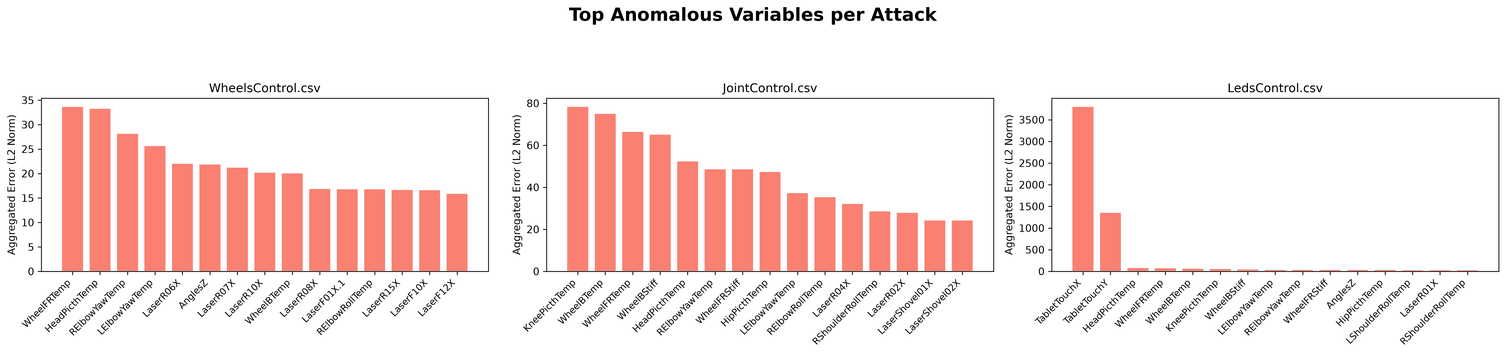
\includegraphics[width=0.85\textwidth,height=0.78\textheight,keepaspectratio]{pcmci_robotic_linear_ridge.png}
  \caption[Attribution: PCMCI, Robotics, linear/ridge]{Top attributed variables per attack class. PCMCI, Robotics domain, linear/ridge.}
  \label{fig:pcmci-robotic-linear-ridge}
\end{figure}

\begin{figure}[htbp]
  \centering
  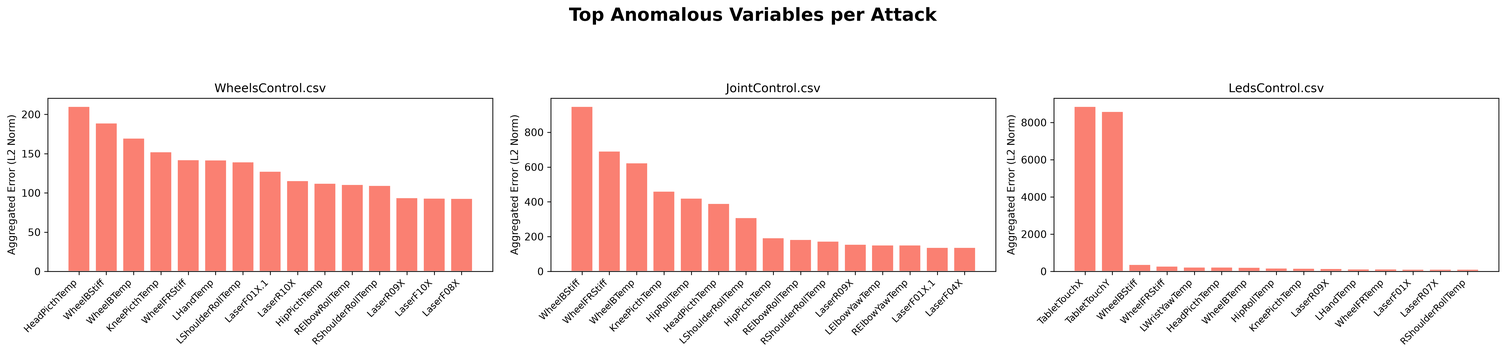
\includegraphics[width=0.85\textwidth,height=0.78\textheight,keepaspectratio]{pcmci_robotic_polynomial_degree_3.png}
  \caption[Attribution: PCMCI, Robotics, polynomial degree 3]{Top attributed variables per attack class. PCMCI, Robotics domain, polynomial degree 3.}
  \label{fig:pcmci-robotic-polynomial-degree-3}
\end{figure}

\begin{figure}[htbp]
  \centering
  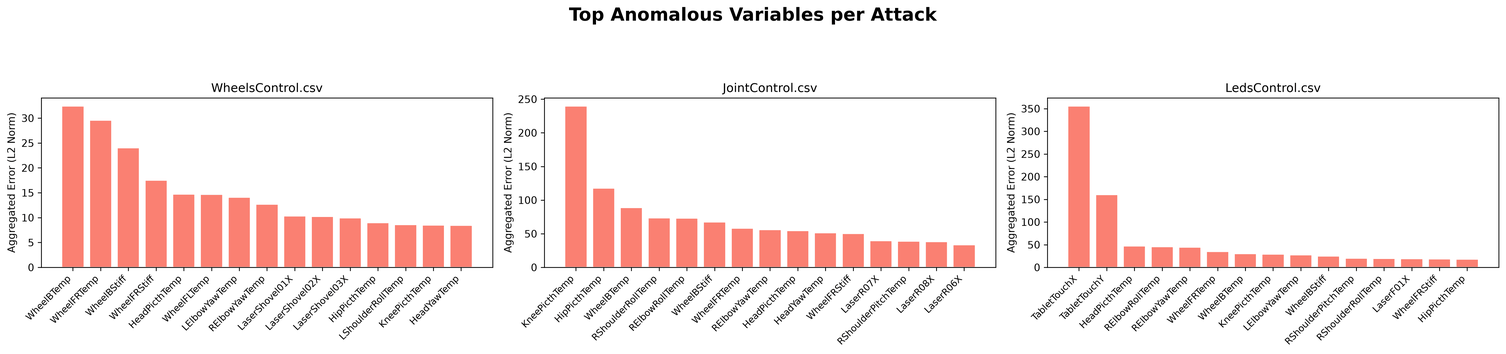
\includegraphics[width=0.85\textwidth,height=0.78\textheight,keepaspectratio]{pcmci_robotic_rbf_ridge.png}
  \caption[Attribution: PCMCI, Robotics, RBF + ridge]{Top attributed variables per attack class. PCMCI, Robotics domain, RBF + ridge.}
  \label{fig:pcmci-robotic-rbf-ridge}
\end{figure}

\begin{figure}[htbp]
  \centering
  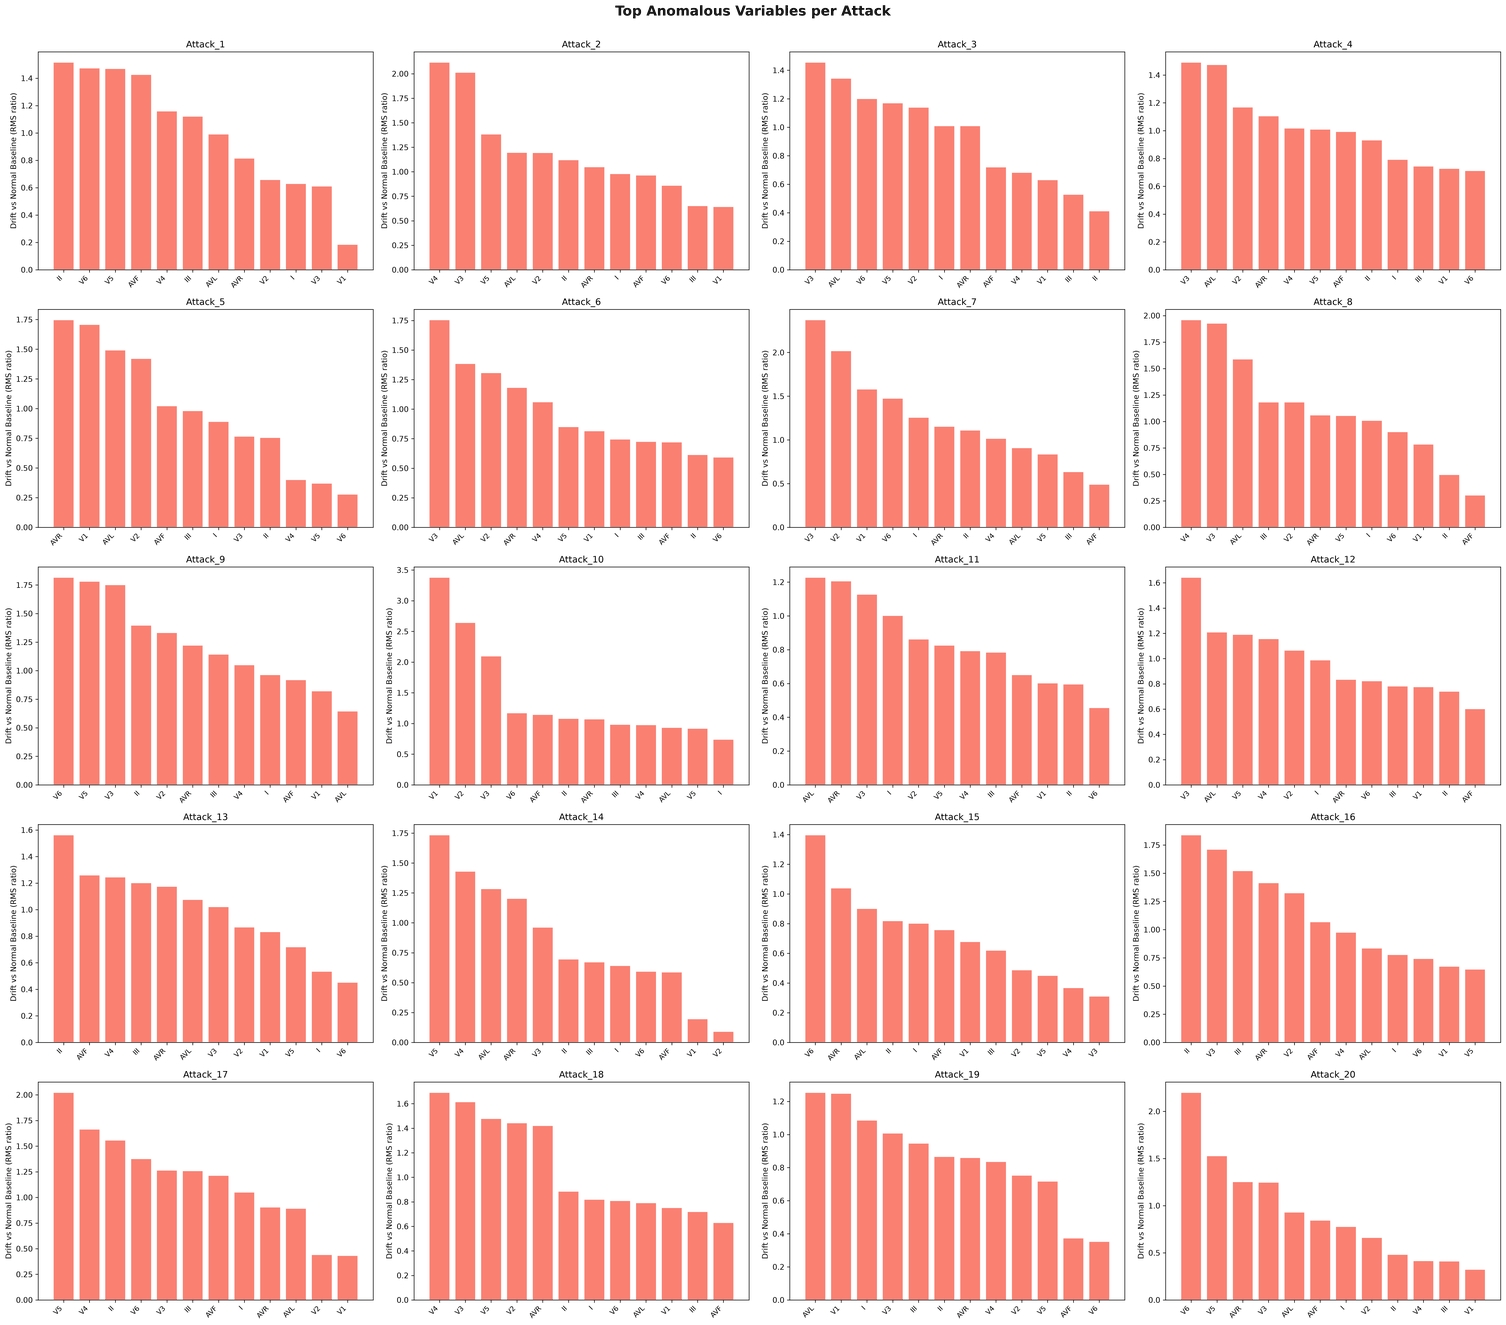
\includegraphics[width=0.85\textwidth,height=0.78\textheight,keepaspectratio]{pcmci_healthcare_linear_ridge.png}
  \caption[Attribution: PCMCI, Healthcare, linear/ridge]{Top attributed variables per attack class. PCMCI, Healthcare domain, linear/ridge.}
  \label{fig:pcmci-healthcare-linear-ridge}
\end{figure}

\begin{figure}[htbp]
  \centering
  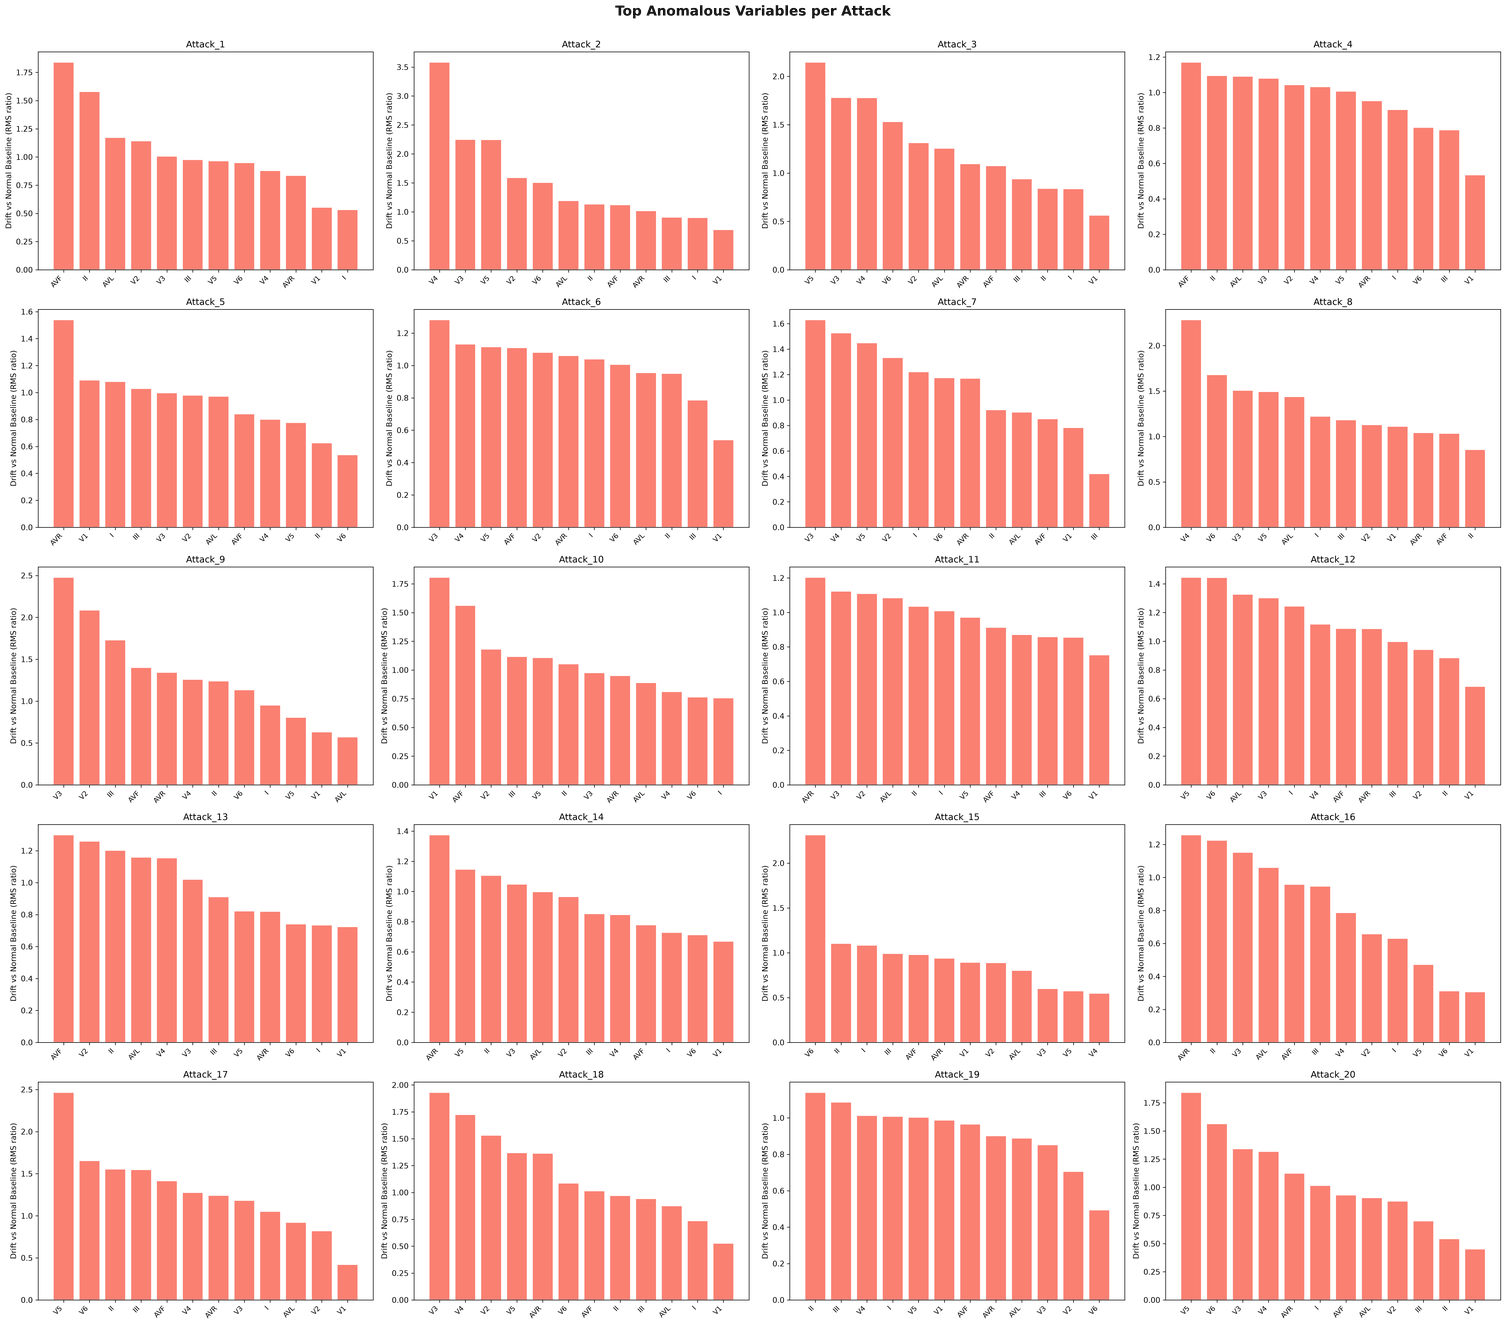
\includegraphics[width=0.85\textwidth,height=0.78\textheight,keepaspectratio]{pcmci_healthcare_polynomial_degree_3.png}
  \caption[Attribution: PCMCI, Healthcare, polynomial degree 3]{Top attributed variables per attack class. PCMCI, Healthcare domain, polynomial degree 3.}
  \label{fig:pcmci-healthcare-polynomial-degree-3}
\end{figure}

\begin{figure}[htbp]
  \centering
  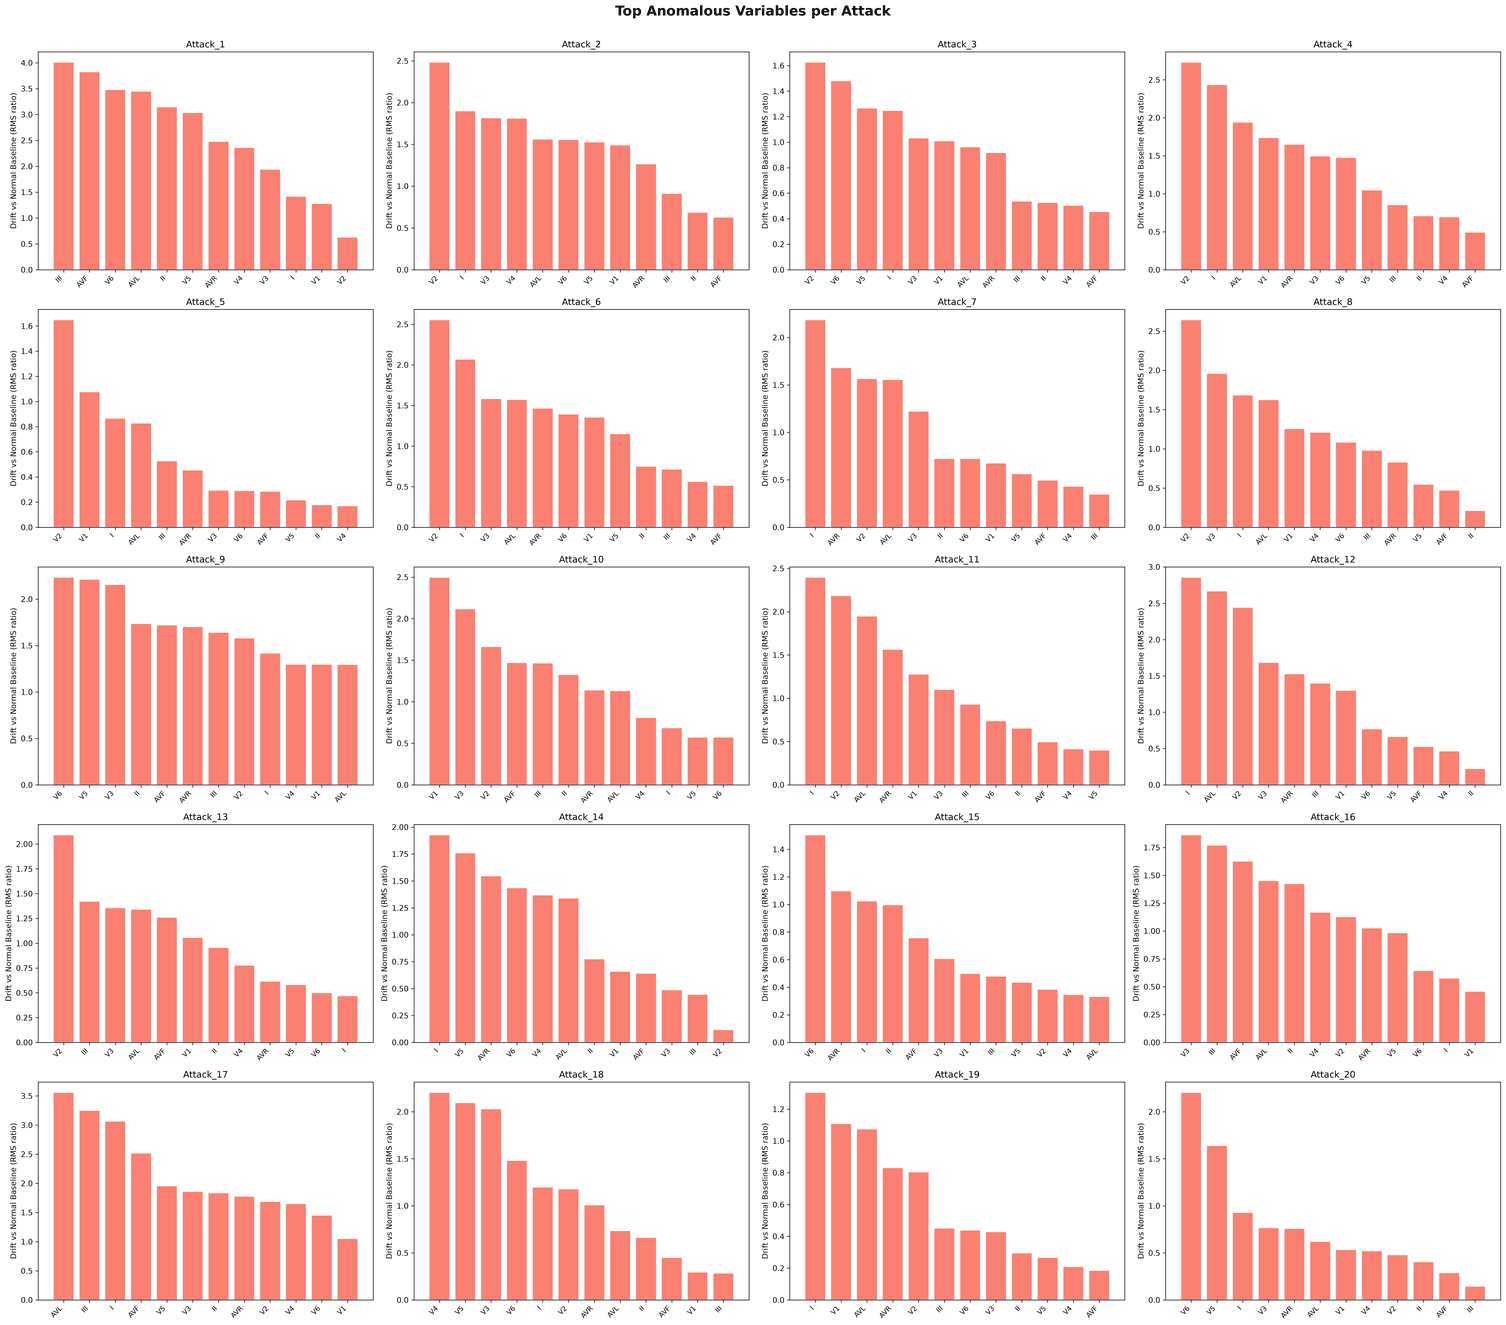
\includegraphics[width=0.85\textwidth,height=0.78\textheight,keepaspectratio]{pcmci_healthcare_rbf_ridge.png}
  \caption[Attribution: PCMCI, Healthcare, RBF + ridge]{Top attributed variables per attack class. PCMCI, Healthcare domain, RBF + ridge.}
  \label{fig:pcmci-healthcare-rbf-ridge}
\end{figure}

\begin{figure}[htbp]
  \centering
  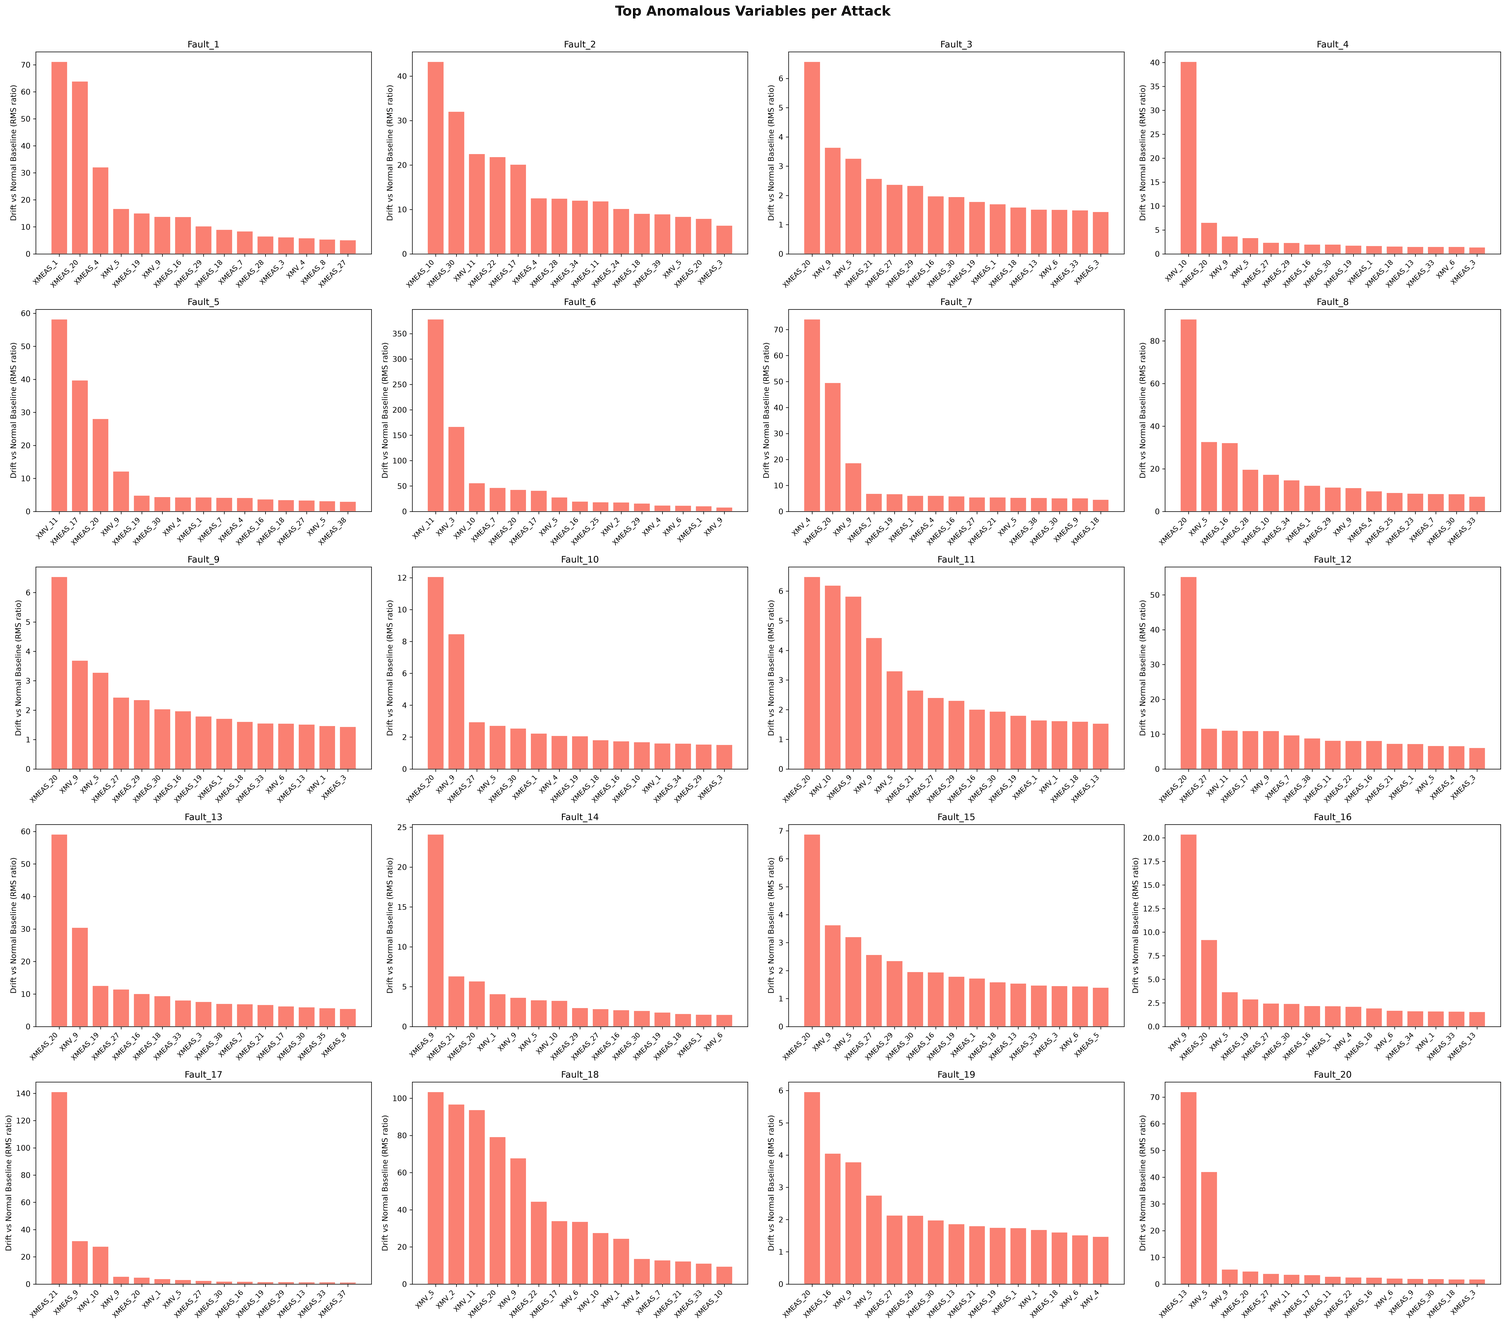
\includegraphics[width=0.85\textwidth,height=0.78\textheight,keepaspectratio]{pcmci_industrial_linear_ridge.png}
  \caption[Attribution: PCMCI, Industrial, linear/ridge]{Top attributed variables per attack class. PCMCI, Industrial domain, linear/ridge.}
  \label{fig:pcmci-industrial-linear-ridge}
\end{figure}

\begin{figure}[htbp]
  \centering
  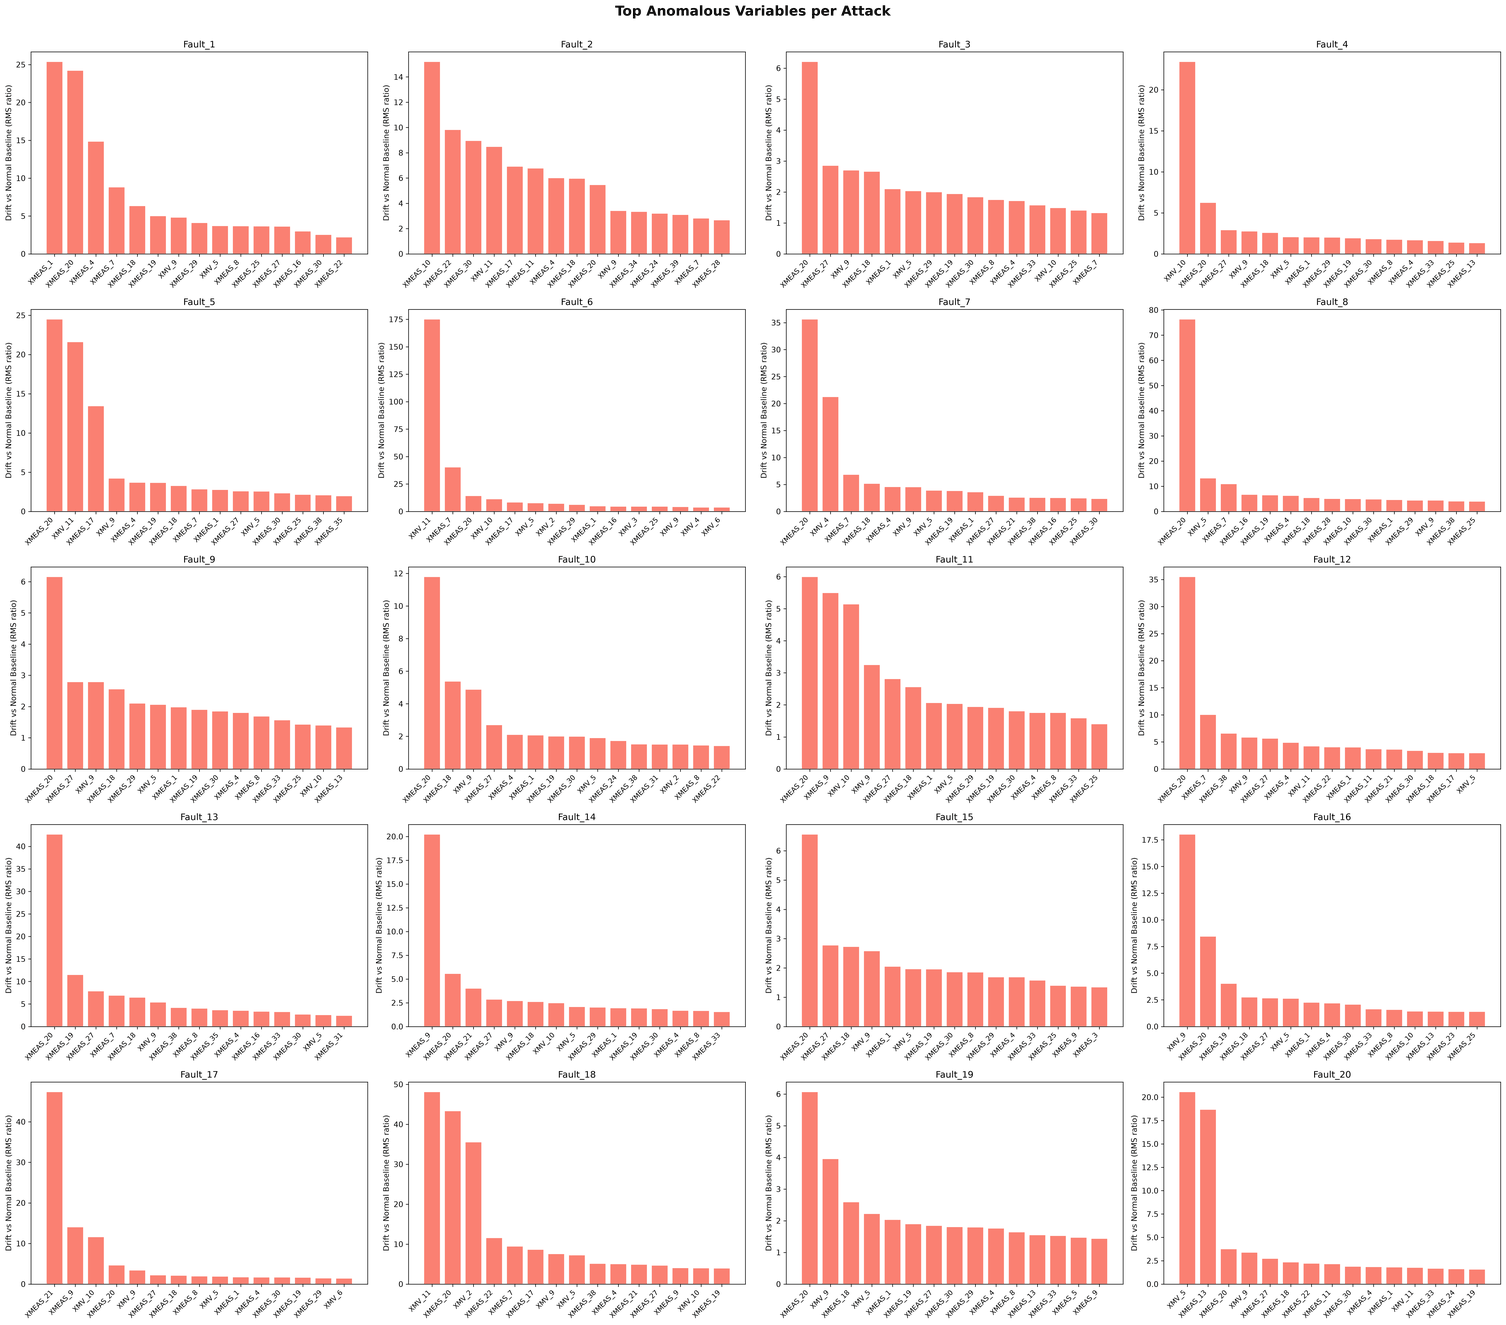
\includegraphics[width=0.85\textwidth,height=0.78\textheight,keepaspectratio]{pcmci_industrial_polynomial_degree_3.png}
  \caption[Attribution: PCMCI, Industrial, polynomial degree 3]{Top attributed variables per attack class. PCMCI, Industrial domain, polynomial degree 3.}
  \label{fig:pcmci-industrial-polynomial-degree-3}
\end{figure}

\begin{figure}[htbp]
  \centering
  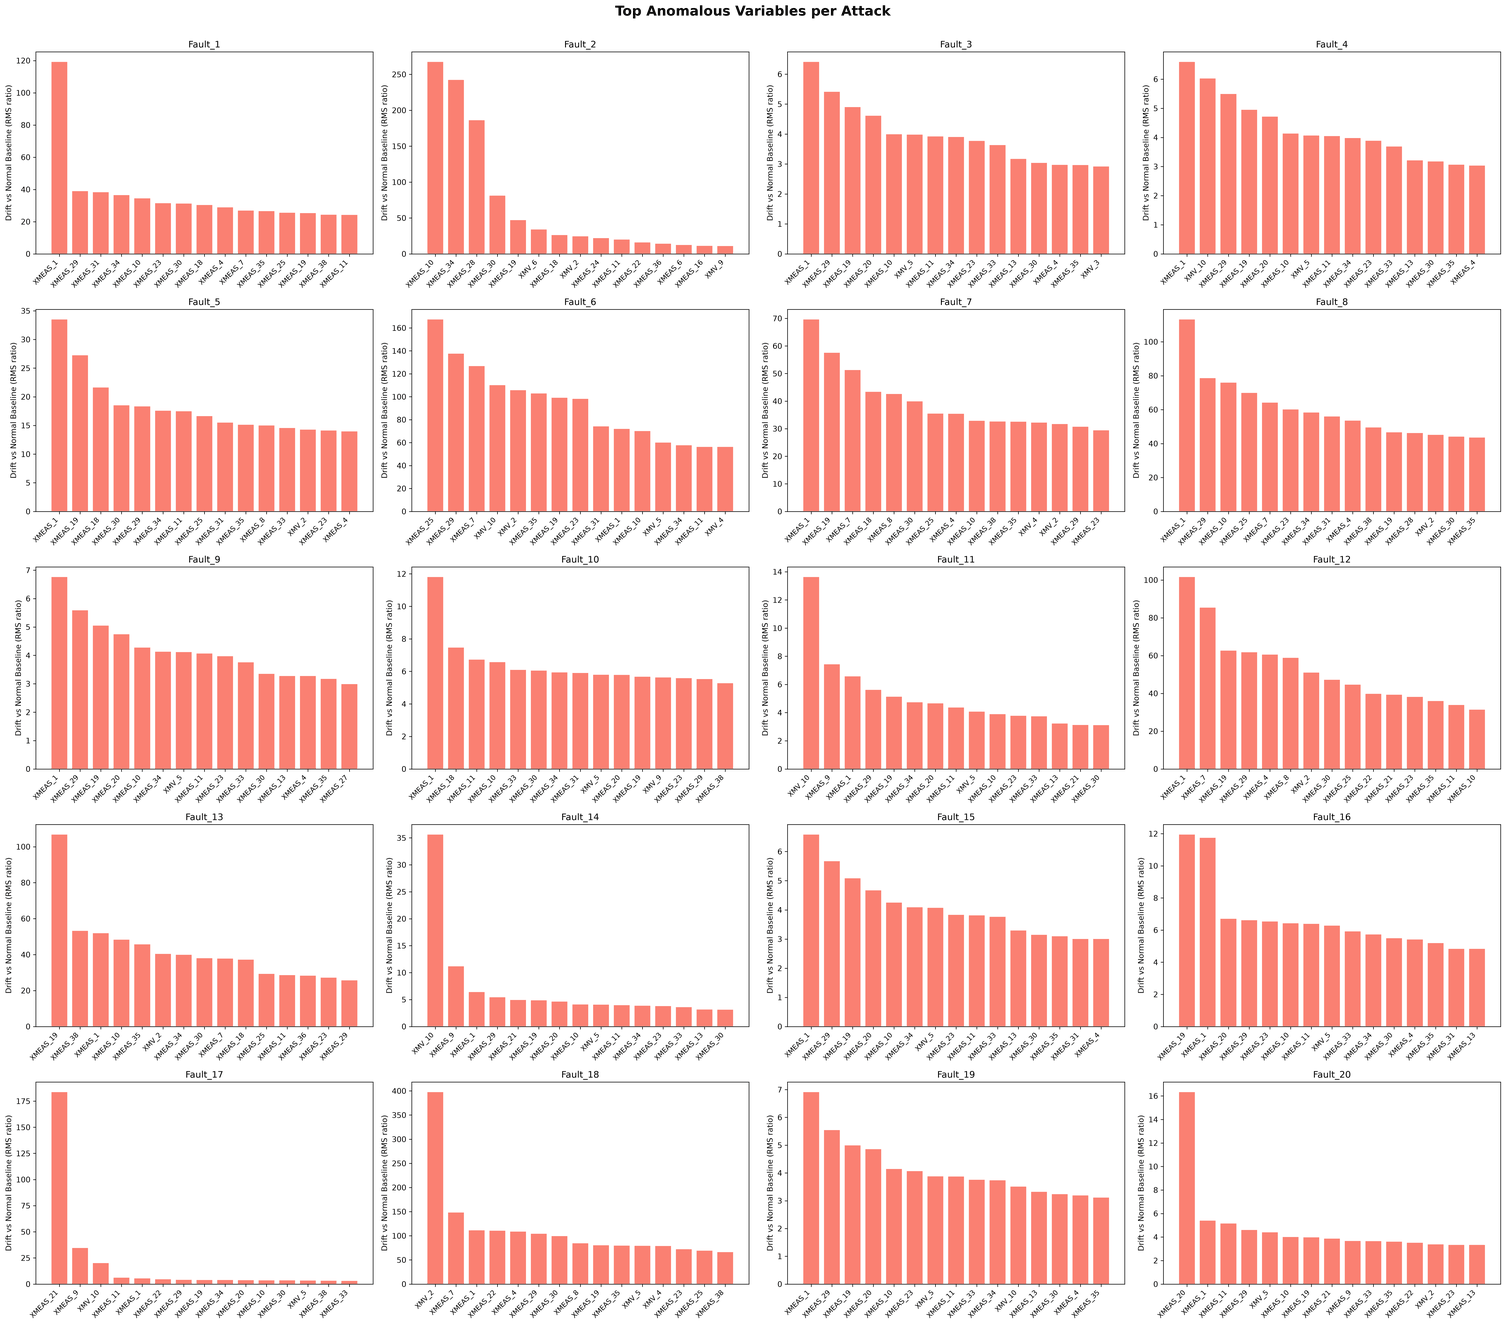
\includegraphics[width=0.85\textwidth,height=0.78\textheight,keepaspectratio]{pcmci_industrial_rbf_ridge.png}
  \caption[Attribution: PCMCI, Industrial, RBF + ridge]{Top attributed variables per attack class. PCMCI, Industrial domain, RBF + ridge.}
  \label{fig:pcmci-industrial-rbf-ridge}
\end{figure}

\begin{figure}[htbp]
  \centering
  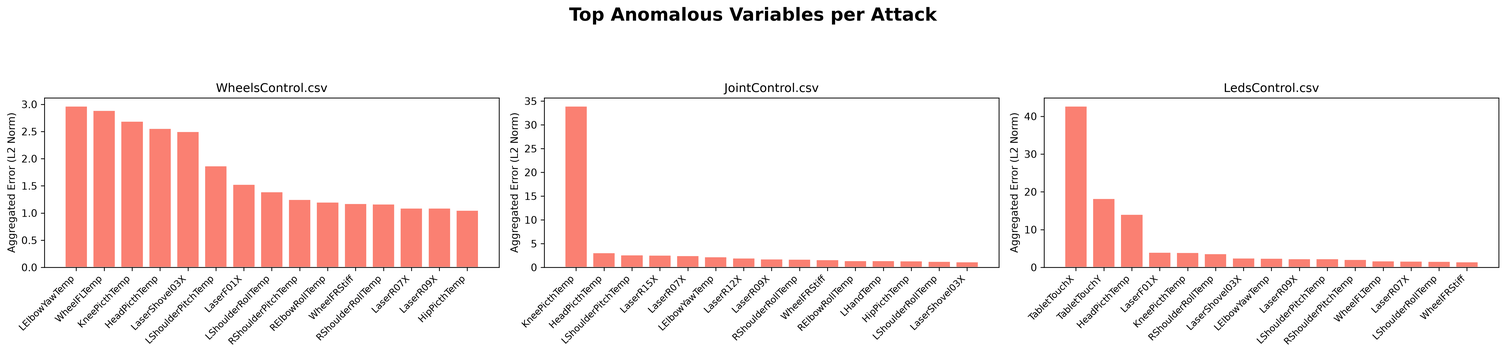
\includegraphics[width=0.85\textwidth,height=0.78\textheight,keepaspectratio]{ges_robotic_linear_ridge.png}
  \caption[Attribution: GES, Robotics, linear/ridge]{Top attributed variables per attack class. GES, Robotics domain, linear/ridge.}
  \label{fig:ges-robotic-linear-ridge}
\end{figure}

\begin{figure}[htbp]
  \centering
  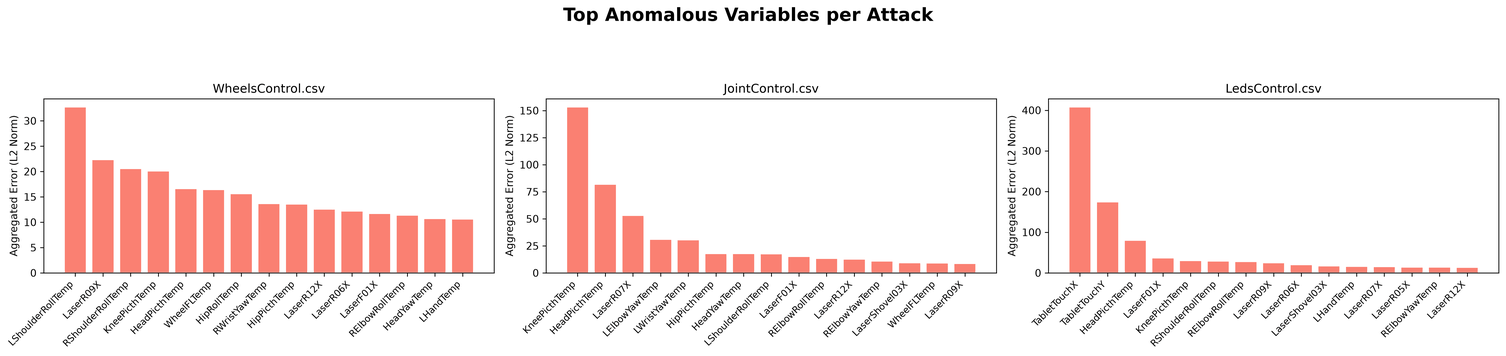
\includegraphics[width=0.85\textwidth,height=0.78\textheight,keepaspectratio]{ges_robotic_polynomial_degree_3.png}
  \caption[Attribution: GES, Robotics, polynomial degree 3]{Top attributed variables per attack class. GES, Robotics domain, polynomial degree 3.}
  \label{fig:ges-robotic-polynomial-degree-3}
\end{figure}

\begin{figure}[htbp]
  \centering
  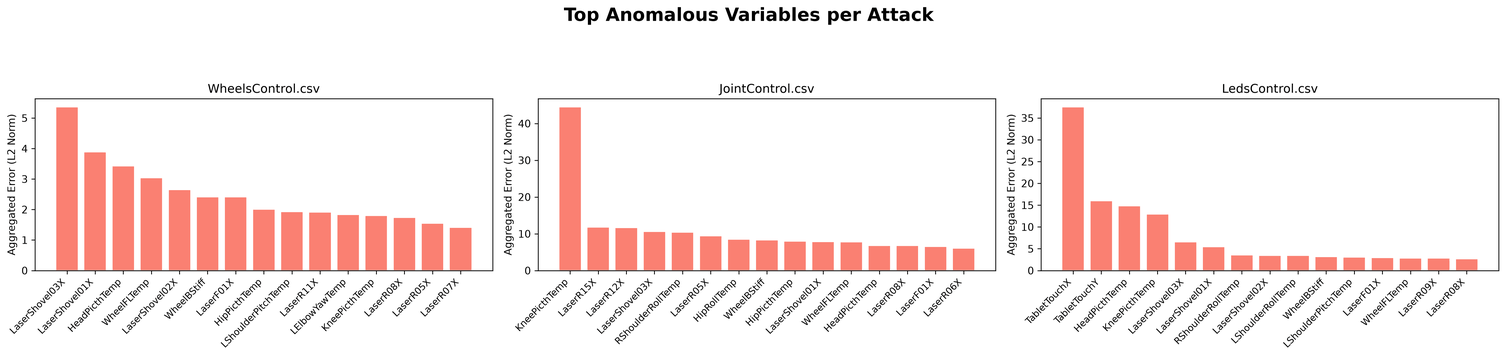
\includegraphics[width=0.85\textwidth,height=0.78\textheight,keepaspectratio]{ges_robotic_rbf_ridge.png}
  \caption[Attribution: GES, Robotics, RBF + ridge]{Top attributed variables per attack class. GES, Robotics domain, RBF + ridge.}
  \label{fig:ges-robotic-rbf-ridge}
\end{figure}

\begin{figure}[htbp]
  \centering
  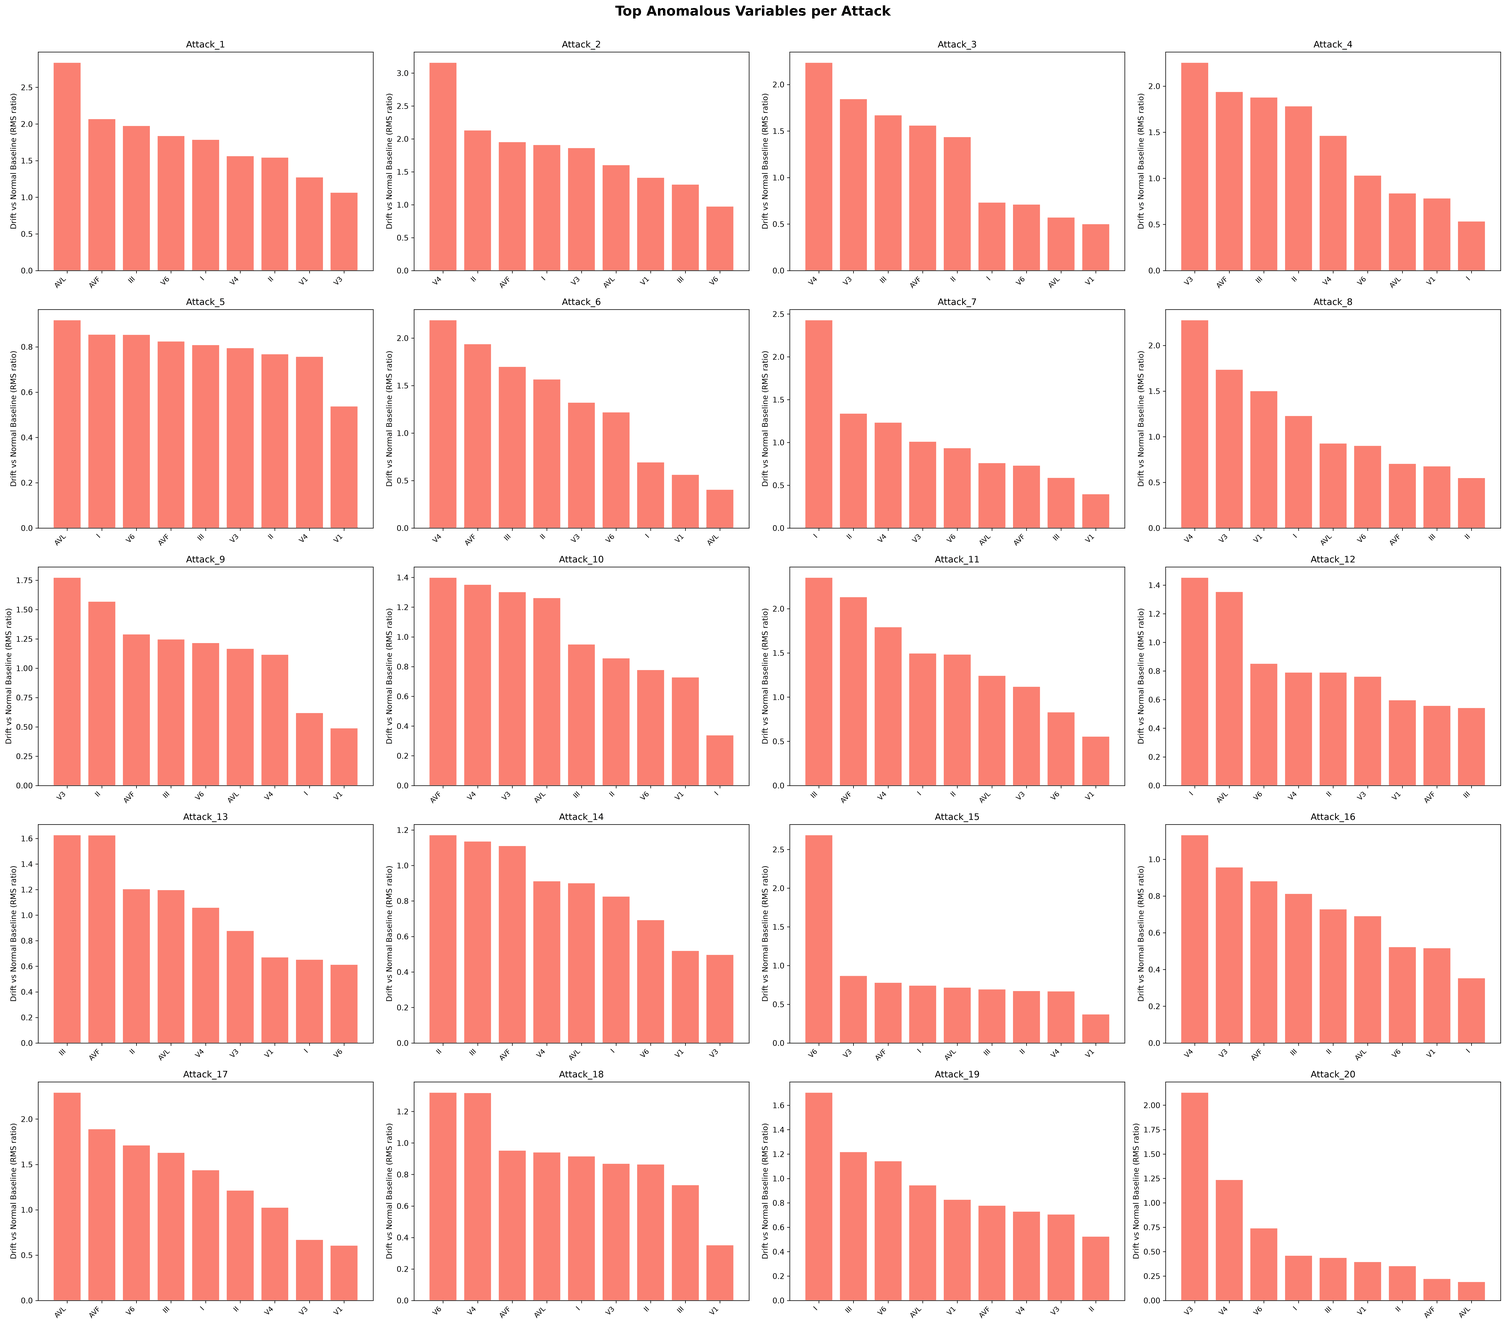
\includegraphics[width=0.85\textwidth,height=0.78\textheight,keepaspectratio]{ges_healthcare_linear_ridge.png}
  \caption[Attribution: GES, Healthcare, linear/ridge]{Top attributed variables per attack class. GES, Healthcare domain, linear/ridge.}
  \label{fig:ges-healthcare-linear-ridge}
\end{figure}

\begin{figure}[htbp]
  \centering
  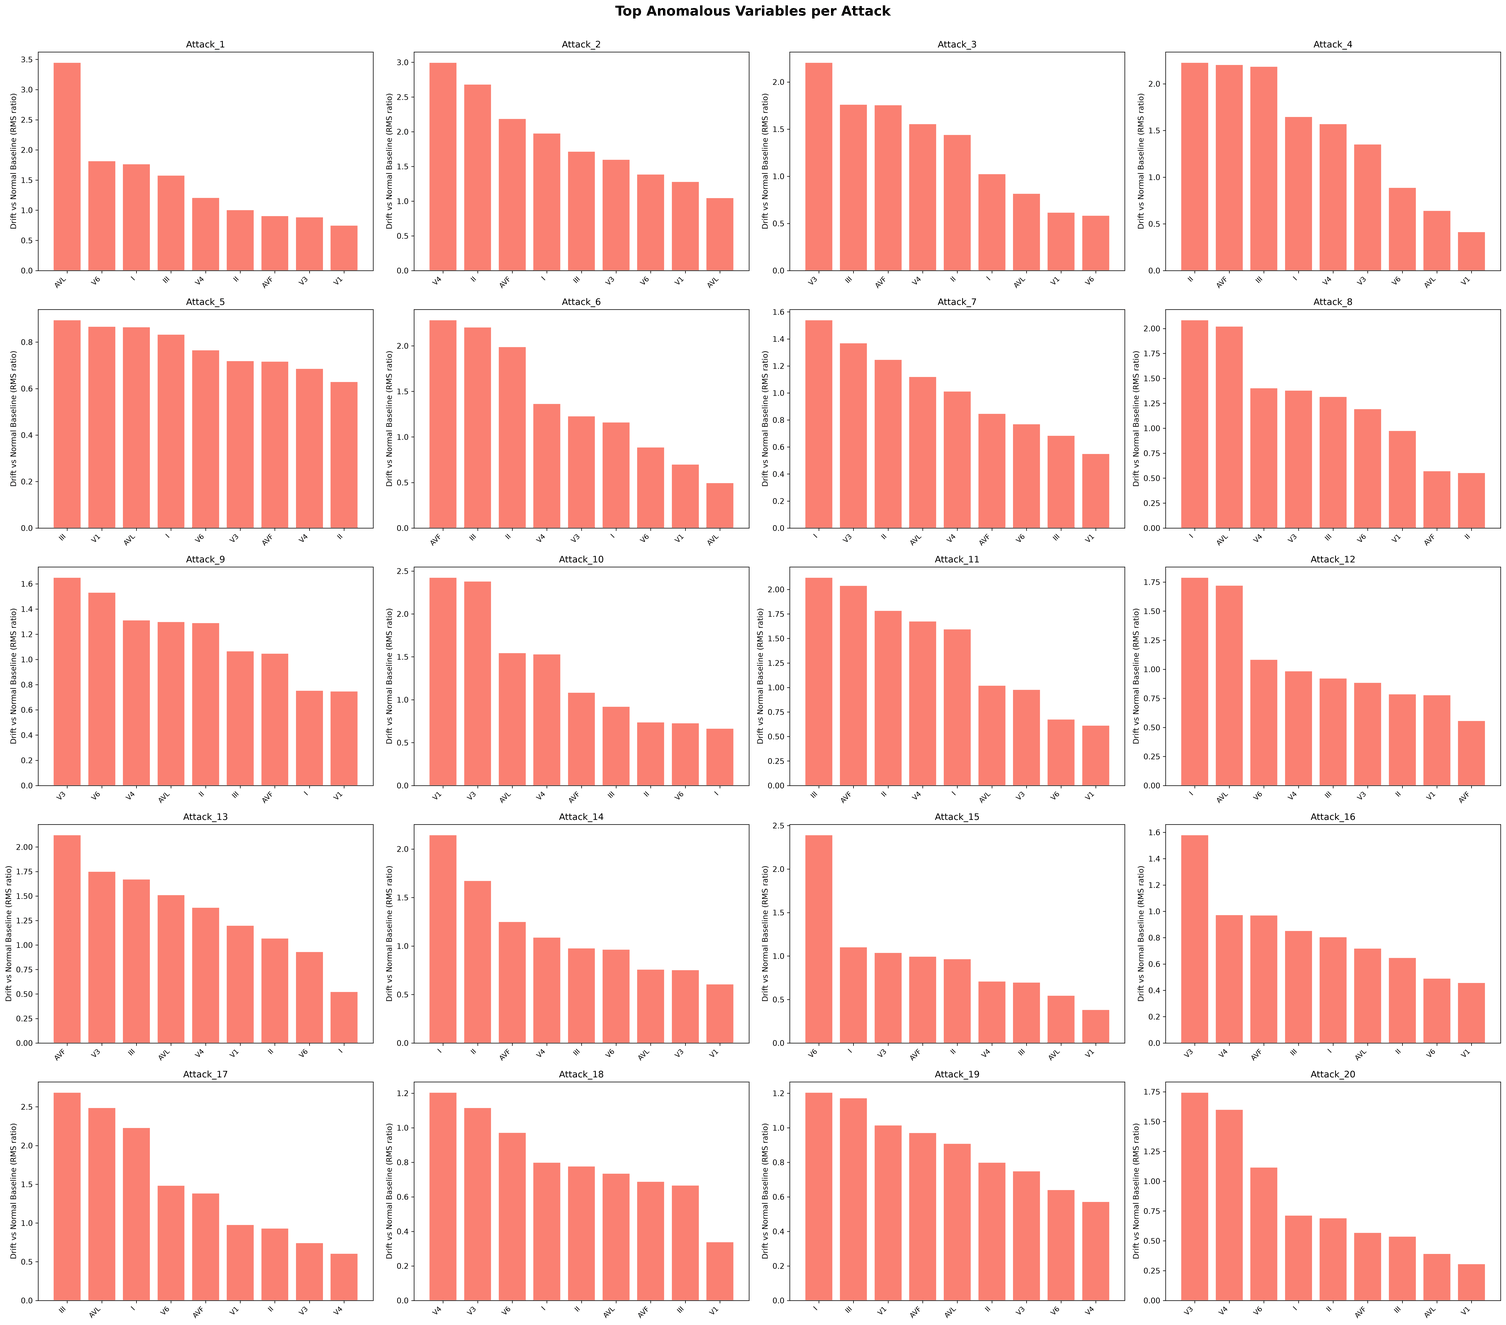
\includegraphics[width=0.85\textwidth,height=0.78\textheight,keepaspectratio]{ges_healthcare_polynomial_degree_3.png}
  \caption[Attribution: GES, Healthcare, polynomial degree 3]{Top attributed variables per attack class. GES, Healthcare domain, polynomial degree 3.}
  \label{fig:ges-healthcare-polynomial-degree-3}
\end{figure}

\begin{figure}[htbp]
  \centering
  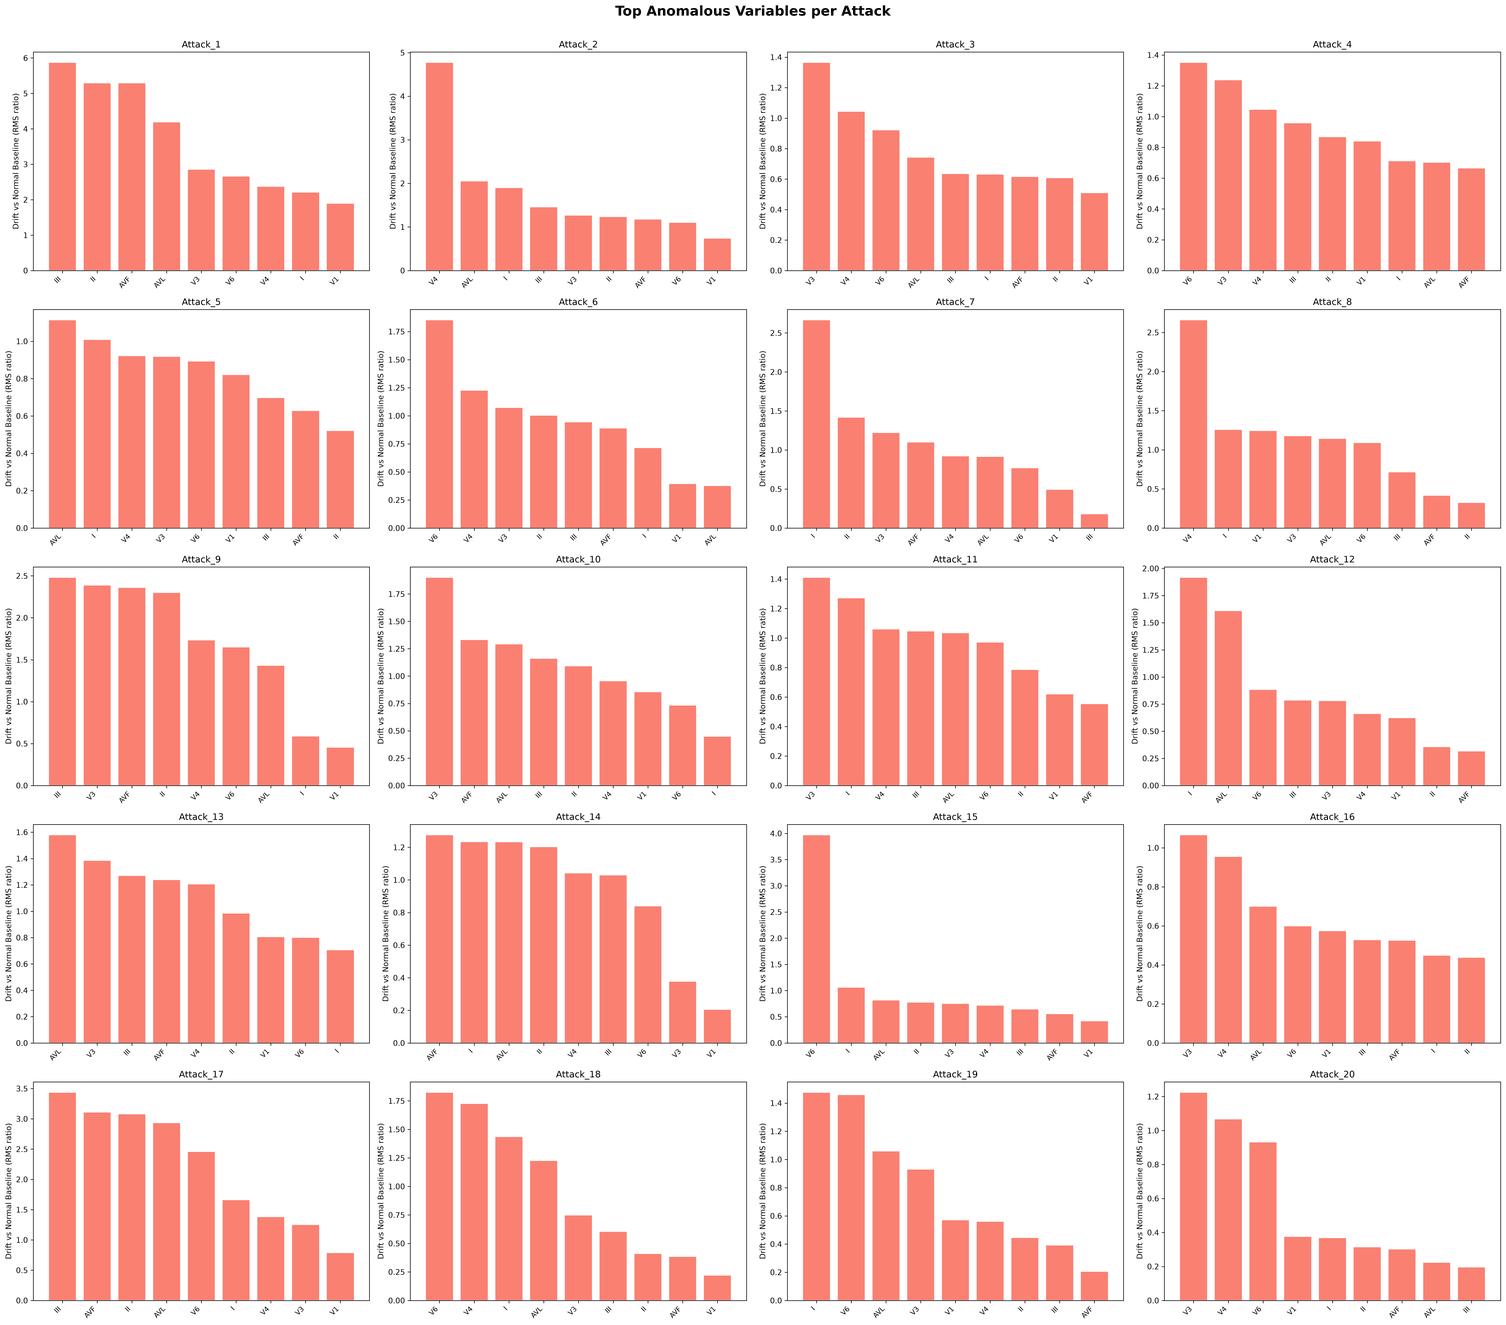
\includegraphics[width=0.85\textwidth,height=0.78\textheight,keepaspectratio]{ges_healthcare_rbf_ridge.png}
  \caption[Attribution: GES, Healthcare, RBF + ridge]{Top attributed variables per attack class. GES, Healthcare domain, RBF + ridge.}
  \label{fig:ges-healthcare-rbf-ridge}
\end{figure}

\begin{figure}[htbp]
  \centering
  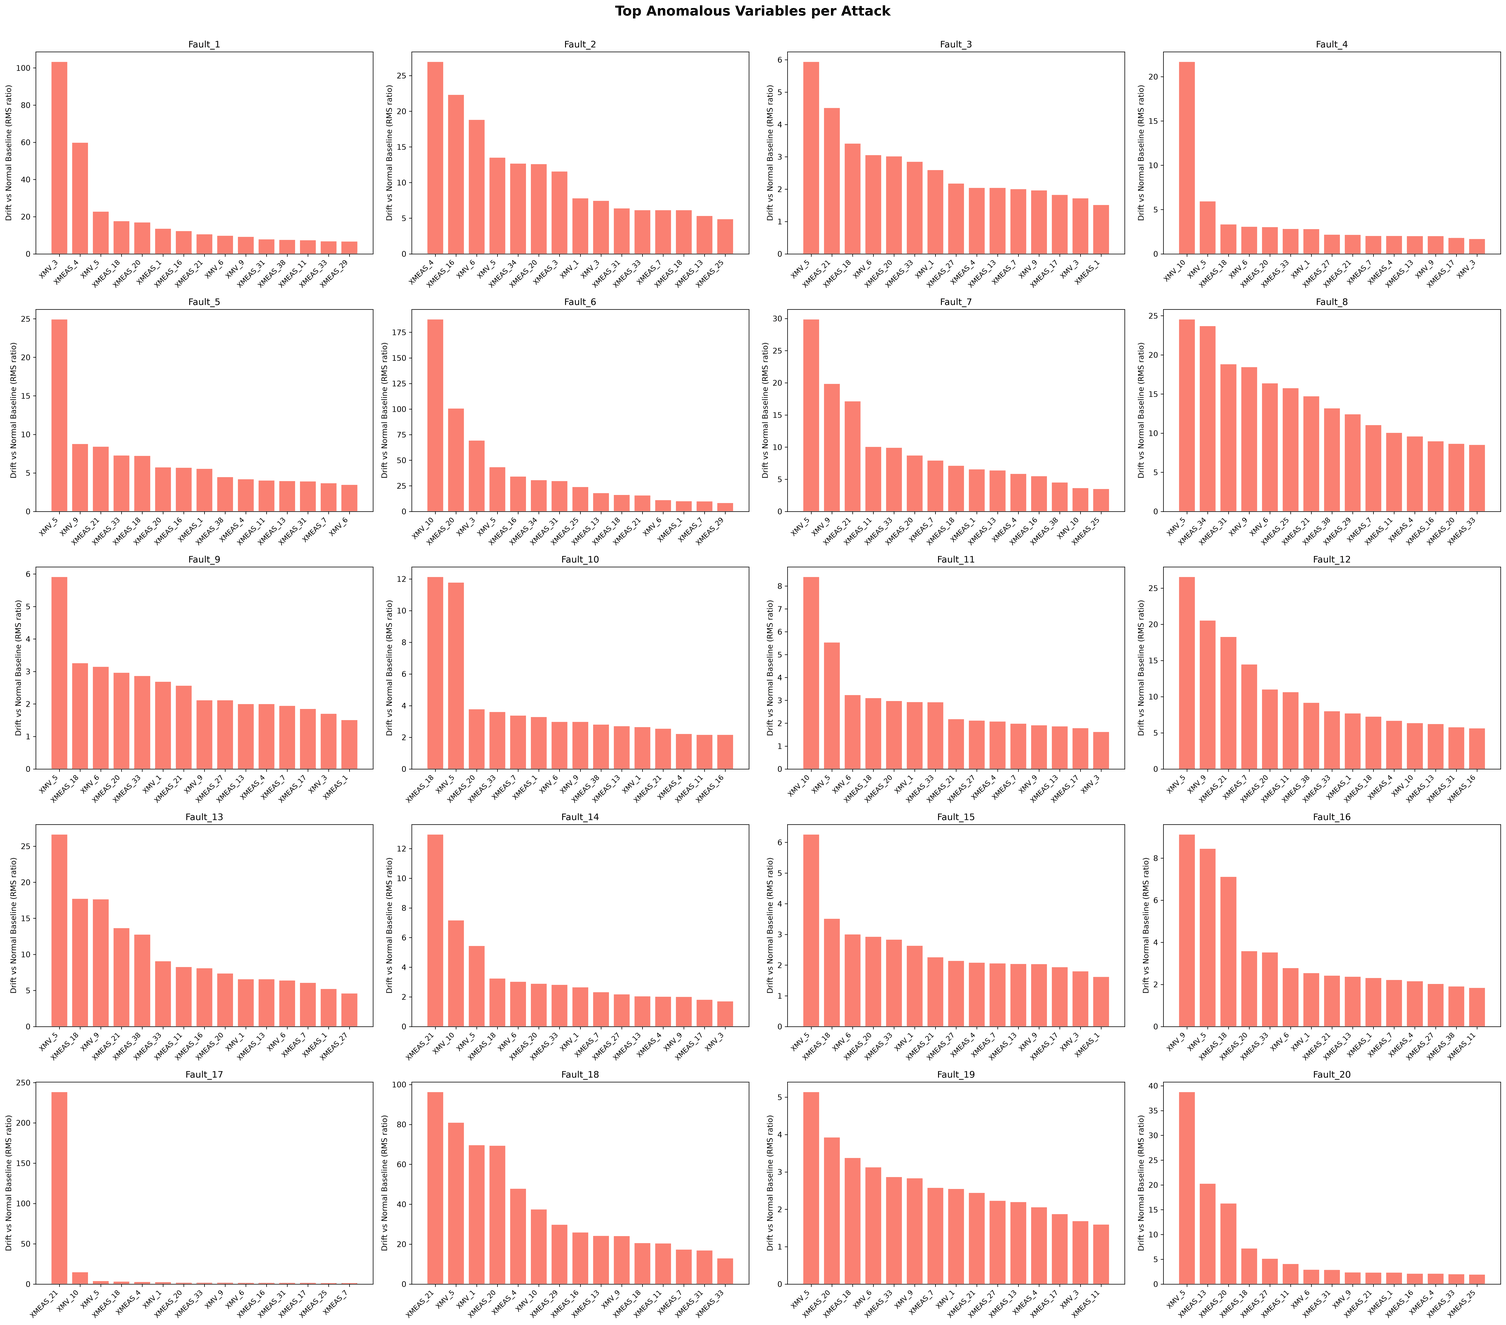
\includegraphics[width=0.85\textwidth,height=0.78\textheight,keepaspectratio]{ges_industrial_linear_ridge.png}
  \caption[Attribution: GES, Industrial, linear/ridge]{Top attributed variables per attack class. GES, Industrial domain, linear/ridge.}
  \label{fig:ges-industrial-linear-ridge}
\end{figure}

\begin{figure}[htbp]
  \centering
  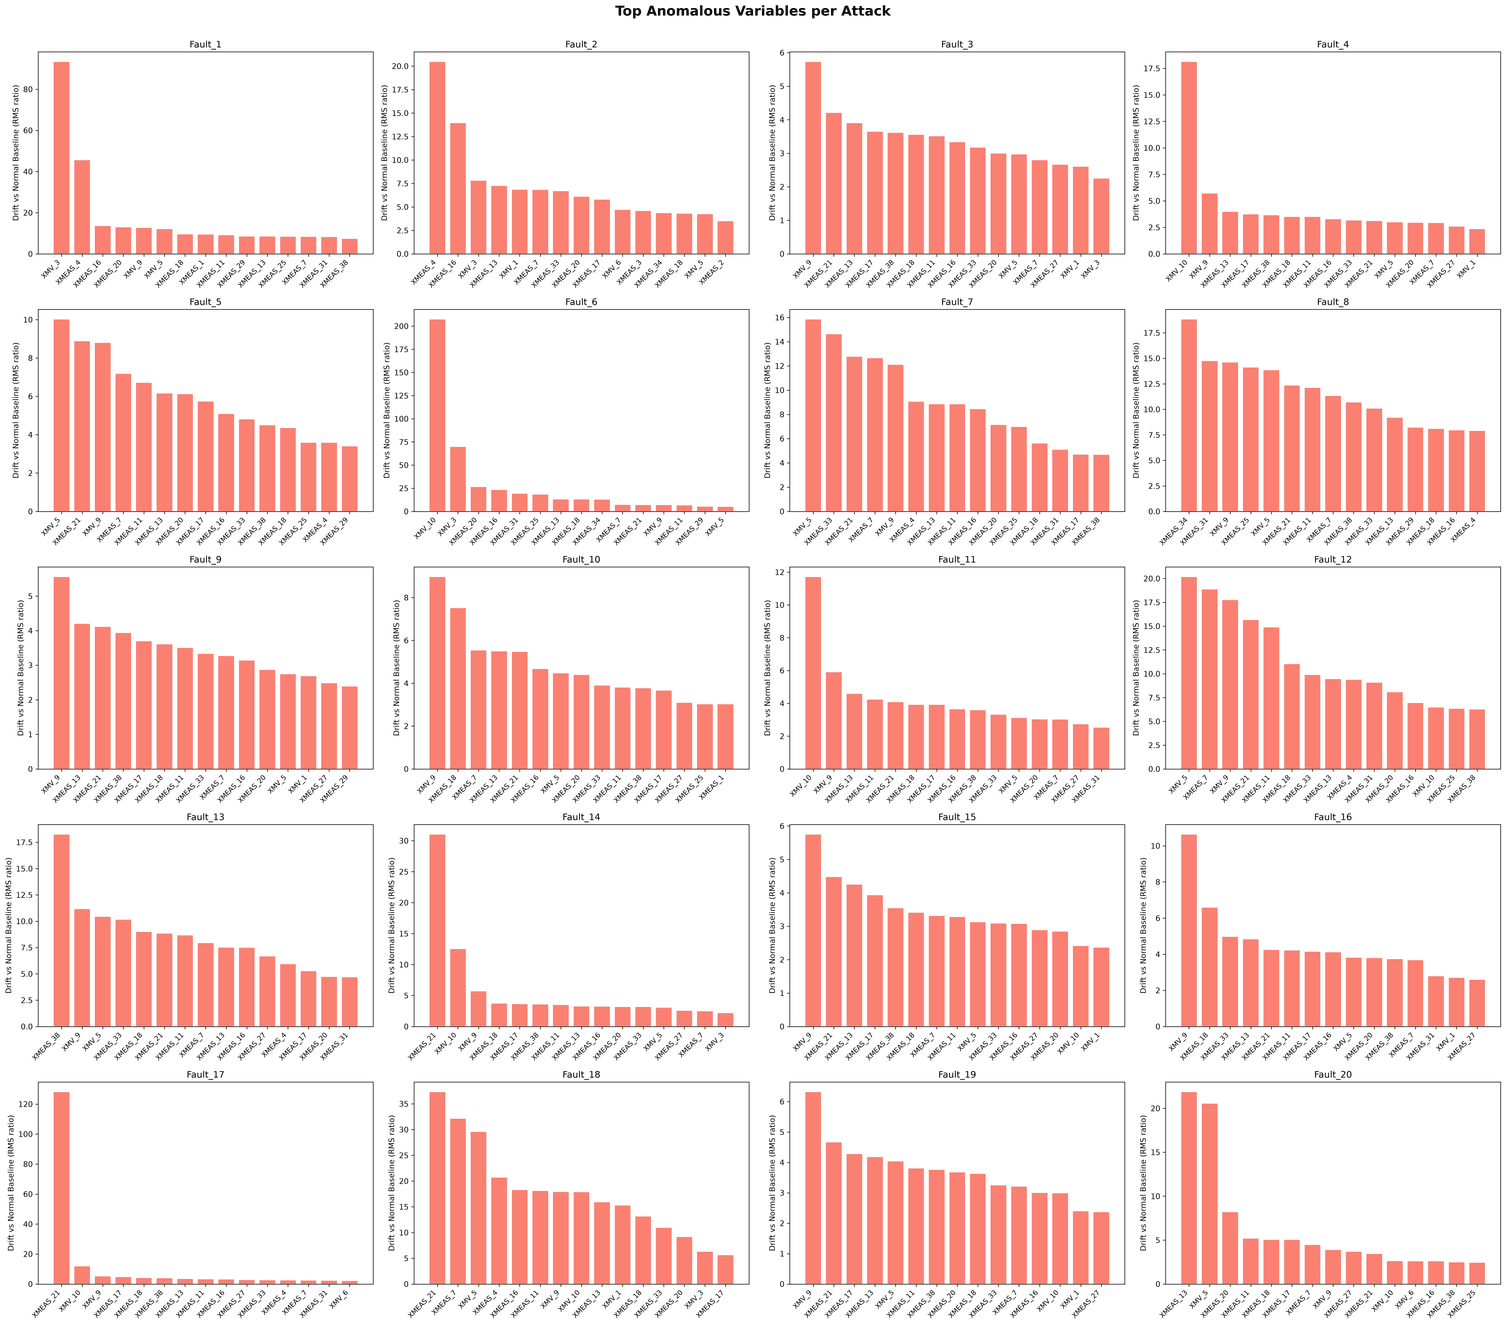
\includegraphics[width=0.85\textwidth,height=0.78\textheight,keepaspectratio]{ges_industrial_polynomial_degree_3.png}
  \caption[Attribution: GES, Industrial, polynomial degree 3]{Top attributed variables per attack class. GES, Industrial domain, polynomial degree 3.}
  \label{fig:ges-industrial-polynomial-degree-3}
\end{figure}

\begin{figure}[htbp]
  \centering
  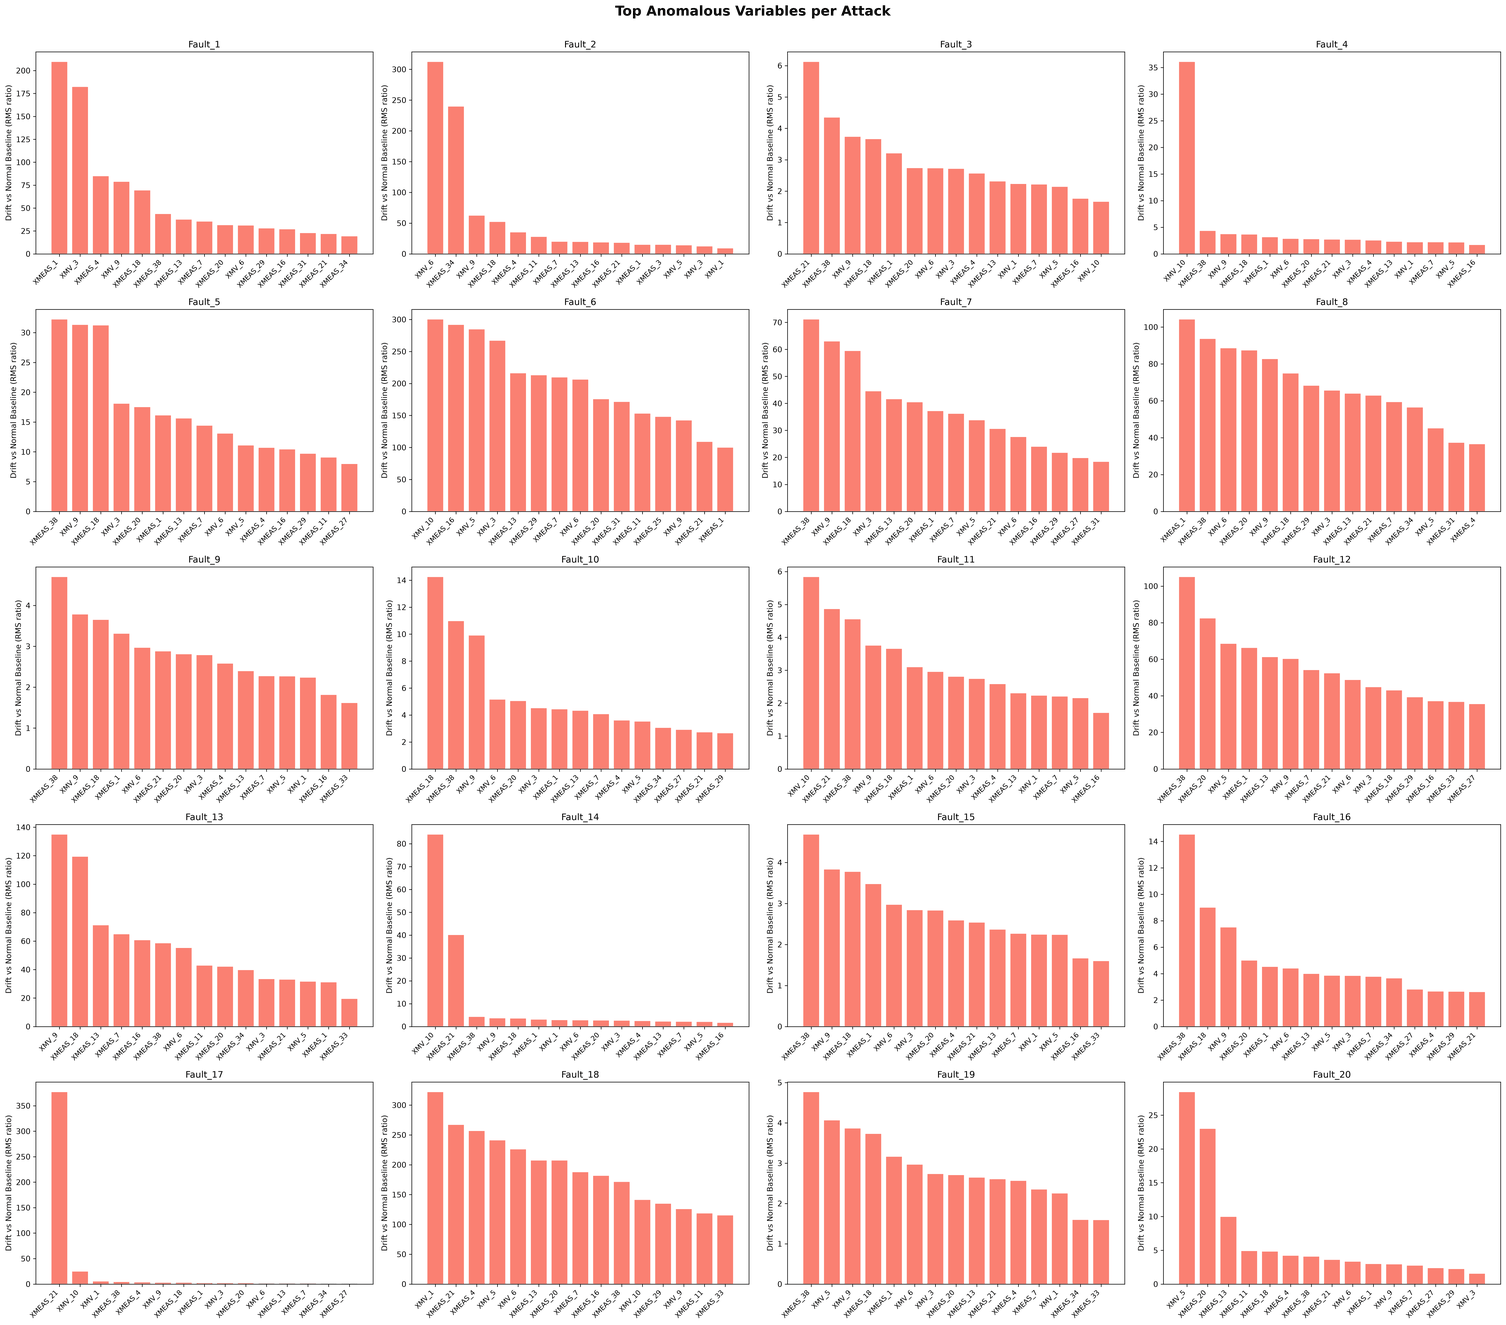
\includegraphics[width=0.85\textwidth,height=0.78\textheight,keepaspectratio]{ges_industrial_rbf_ridge.png}
  \caption[Attribution: GES, Industrial, RBF + ridge]{Top attributed variables per attack class. GES, Industrial domain, RBF + ridge.}
  \label{fig:ges-industrial-rbf-ridge}
\end{figure}

\begin{figure}[htbp]
  \centering
  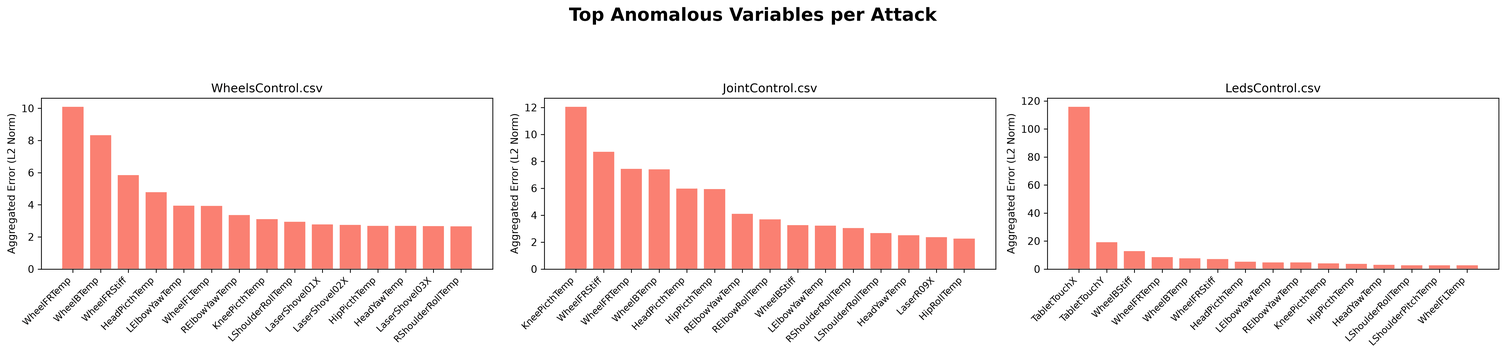
\includegraphics[width=0.85\textwidth,height=0.78\textheight,keepaspectratio]{camuv_robotics_linear_ridge.png}
  \caption[Attribution: CAM-UV, Robotics, linear/ridge]{Top attributed variables per attack class. CAM-UV, Robotics domain, linear/ridge.}
  \label{fig:camuv-robotics-linear-ridge}
\end{figure}

\begin{figure}[htbp]
  \centering
  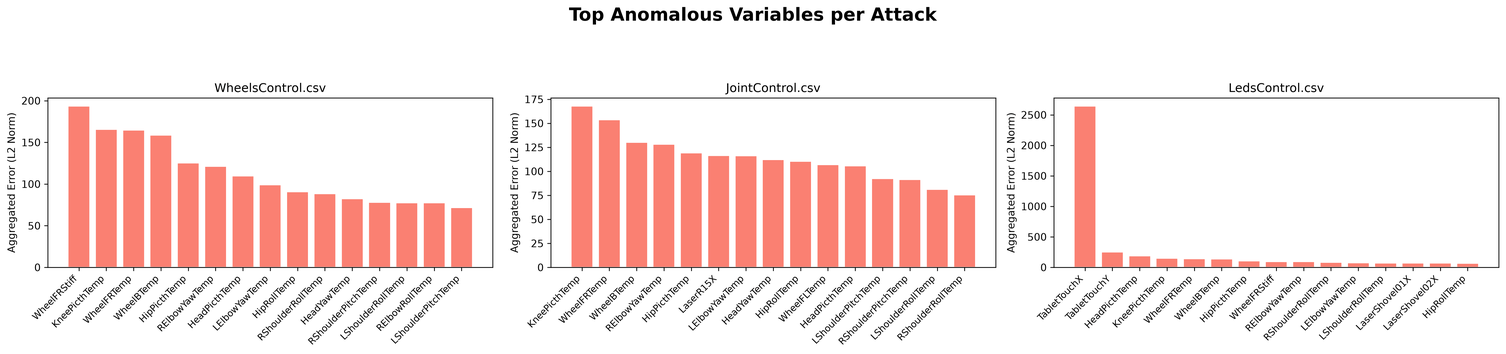
\includegraphics[width=0.85\textwidth,height=0.78\textheight,keepaspectratio]{camuv_robotics_polynomial_degree_3.png}
  \caption[Attribution: CAM-UV, Robotics, polynomial degree 3]{Top attributed variables per attack class. CAM-UV, Robotics domain, polynomial degree 3.}
  \label{fig:camuv-robotics-polynomial-degree-3}
\end{figure}

\begin{figure}[htbp]
  \centering
  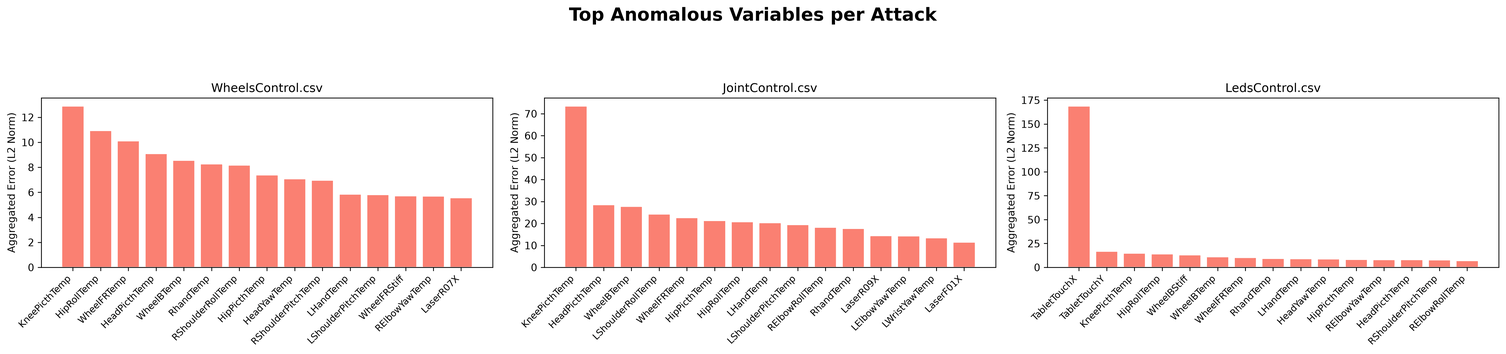
\includegraphics[width=0.85\textwidth,height=0.78\textheight,keepaspectratio]{camuv_robotics_rbf_ridge.png}
  \caption[Attribution: CAM-UV, Robotics, RBF + ridge]{Top attributed variables per attack class. CAM-UV, Robotics domain, RBF + ridge.}
  \label{fig:camuv-robotics-rbf-ridge}
\end{figure}

\begin{figure}[htbp]
  \centering
  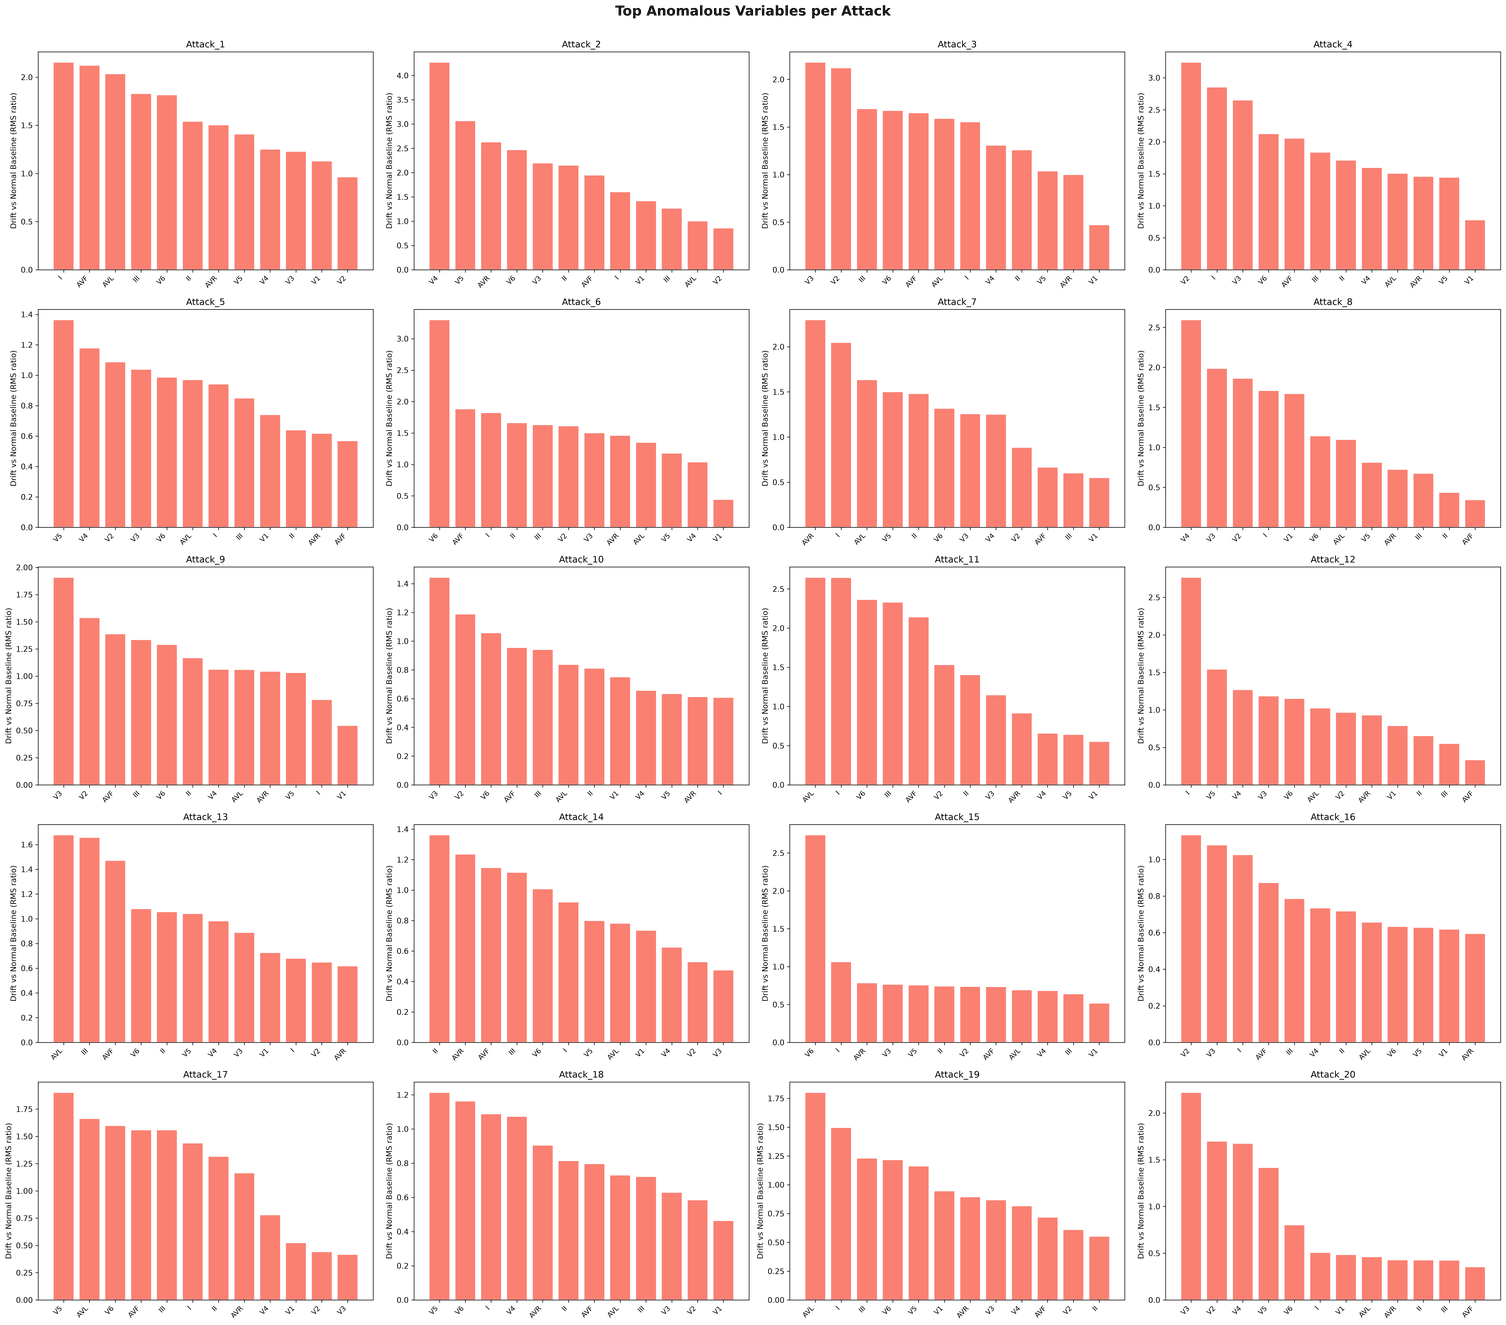
\includegraphics[width=0.85\textwidth,height=0.78\textheight,keepaspectratio]{camuv_healthcare_linear_ridge.png}
  \caption[Attribution: CAM-UV, Healthcare, linear/ridge]{Top attributed variables per attack class. CAM-UV, Healthcare domain, linear/ridge.}
  \label{fig:camuv-healthcare-linear-ridge}
\end{figure}

\begin{figure}[htbp]
  \centering
  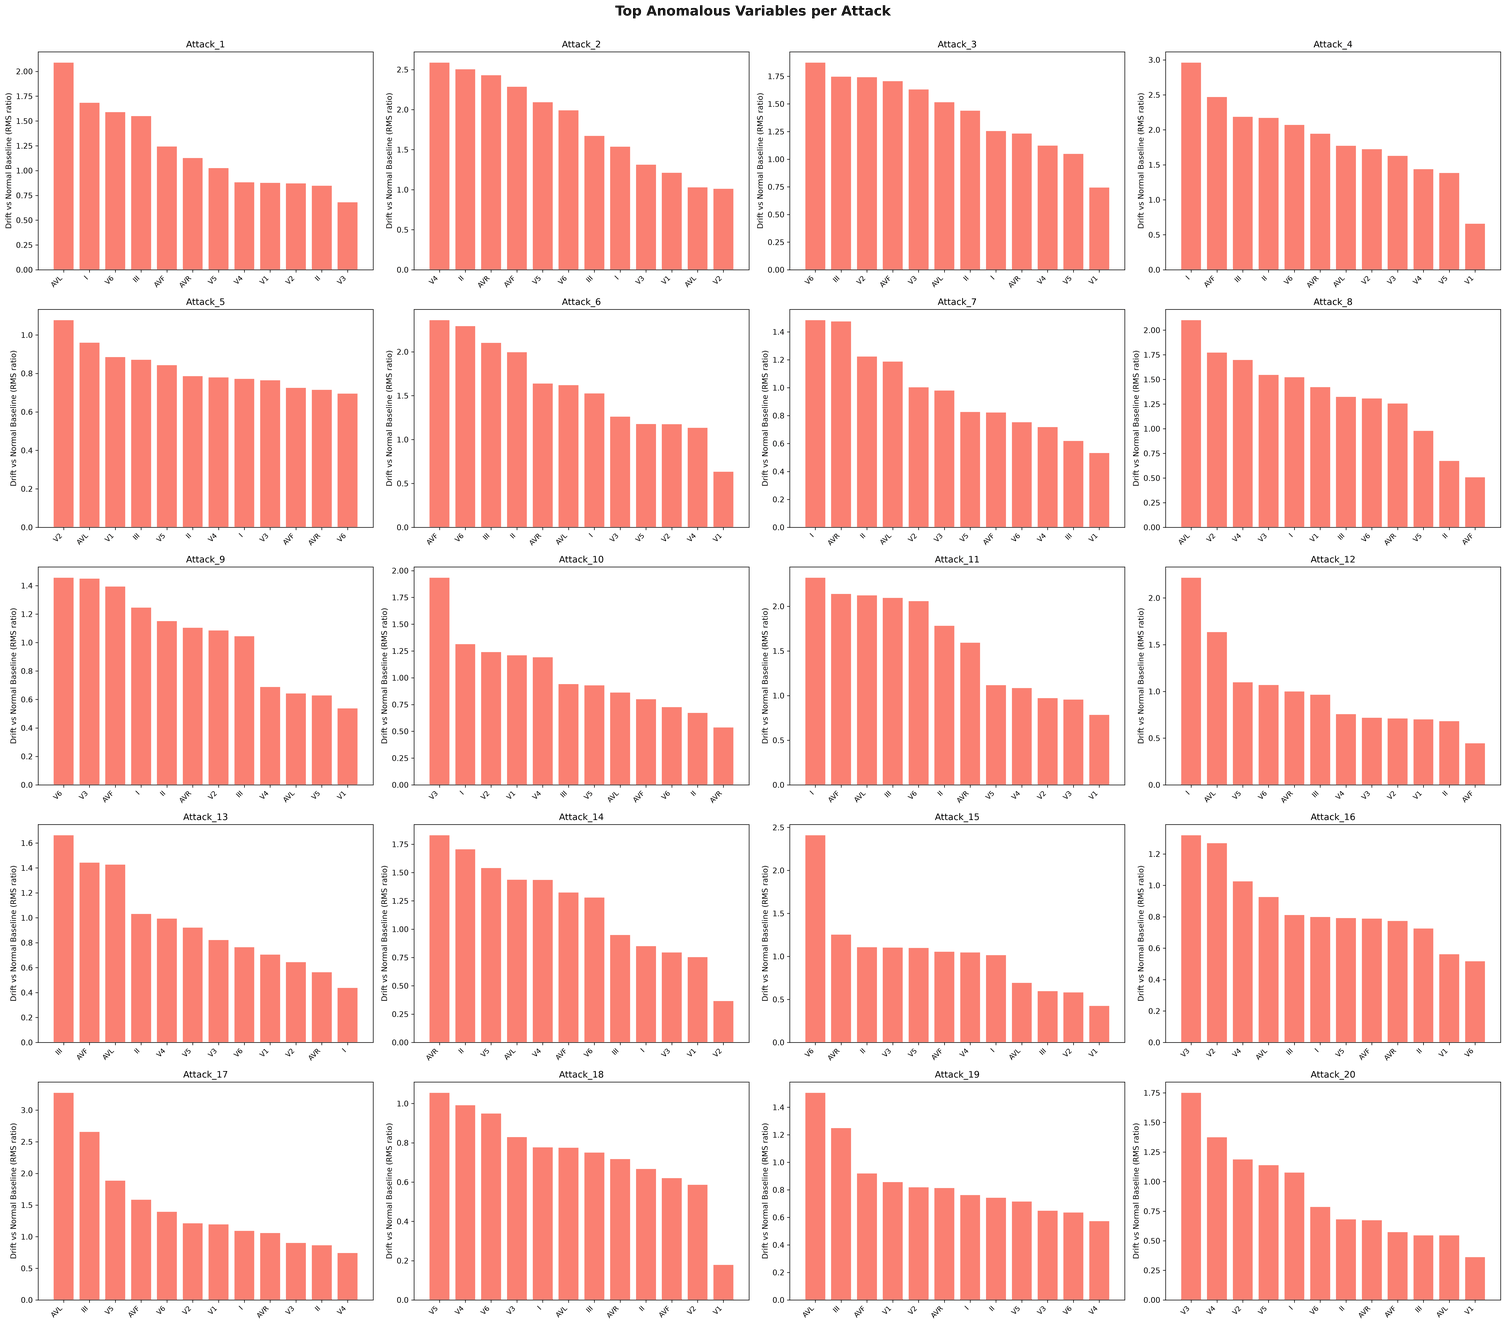
\includegraphics[width=0.85\textwidth,height=0.78\textheight,keepaspectratio]{camuv_healthcare_polynomial_degree_3.png}
  \caption[Attribution: CAM-UV, Healthcare, polynomial degree 3]{Top attributed variables per attack class. CAM-UV, Healthcare domain, polynomial degree 3.}
  \label{fig:camuv-healthcare-polynomial-degree-3}
\end{figure}

\begin{figure}[htbp]
  \centering
  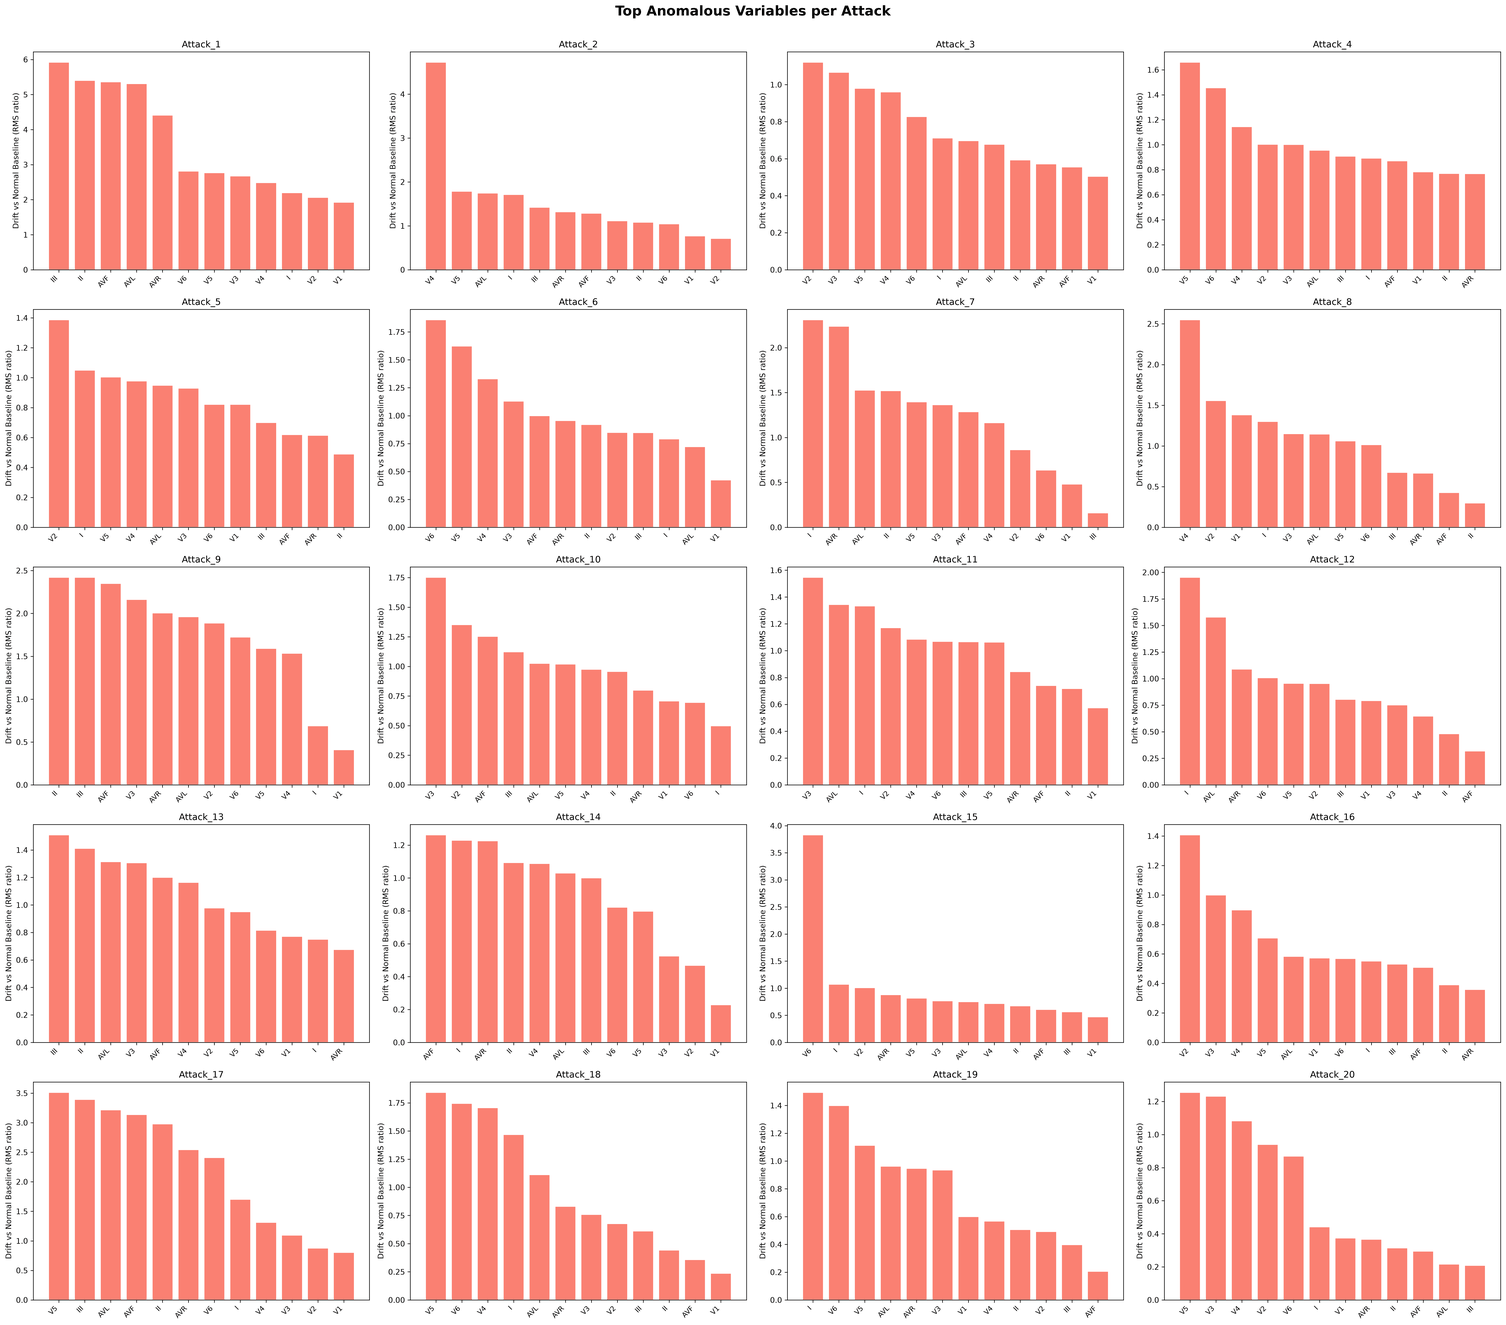
\includegraphics[width=0.85\textwidth,height=0.78\textheight,keepaspectratio]{camuv_healthcare_rbf_ridge.png}
  \caption[Attribution: CAM-UV, Healthcare, RBF + ridge]{Top attributed variables per attack class. CAM-UV, Healthcare domain, RBF + ridge.}
  \label{fig:camuv-healthcare-rbf-ridge}
\end{figure}

\begin{figure}[htbp]
  \centering
  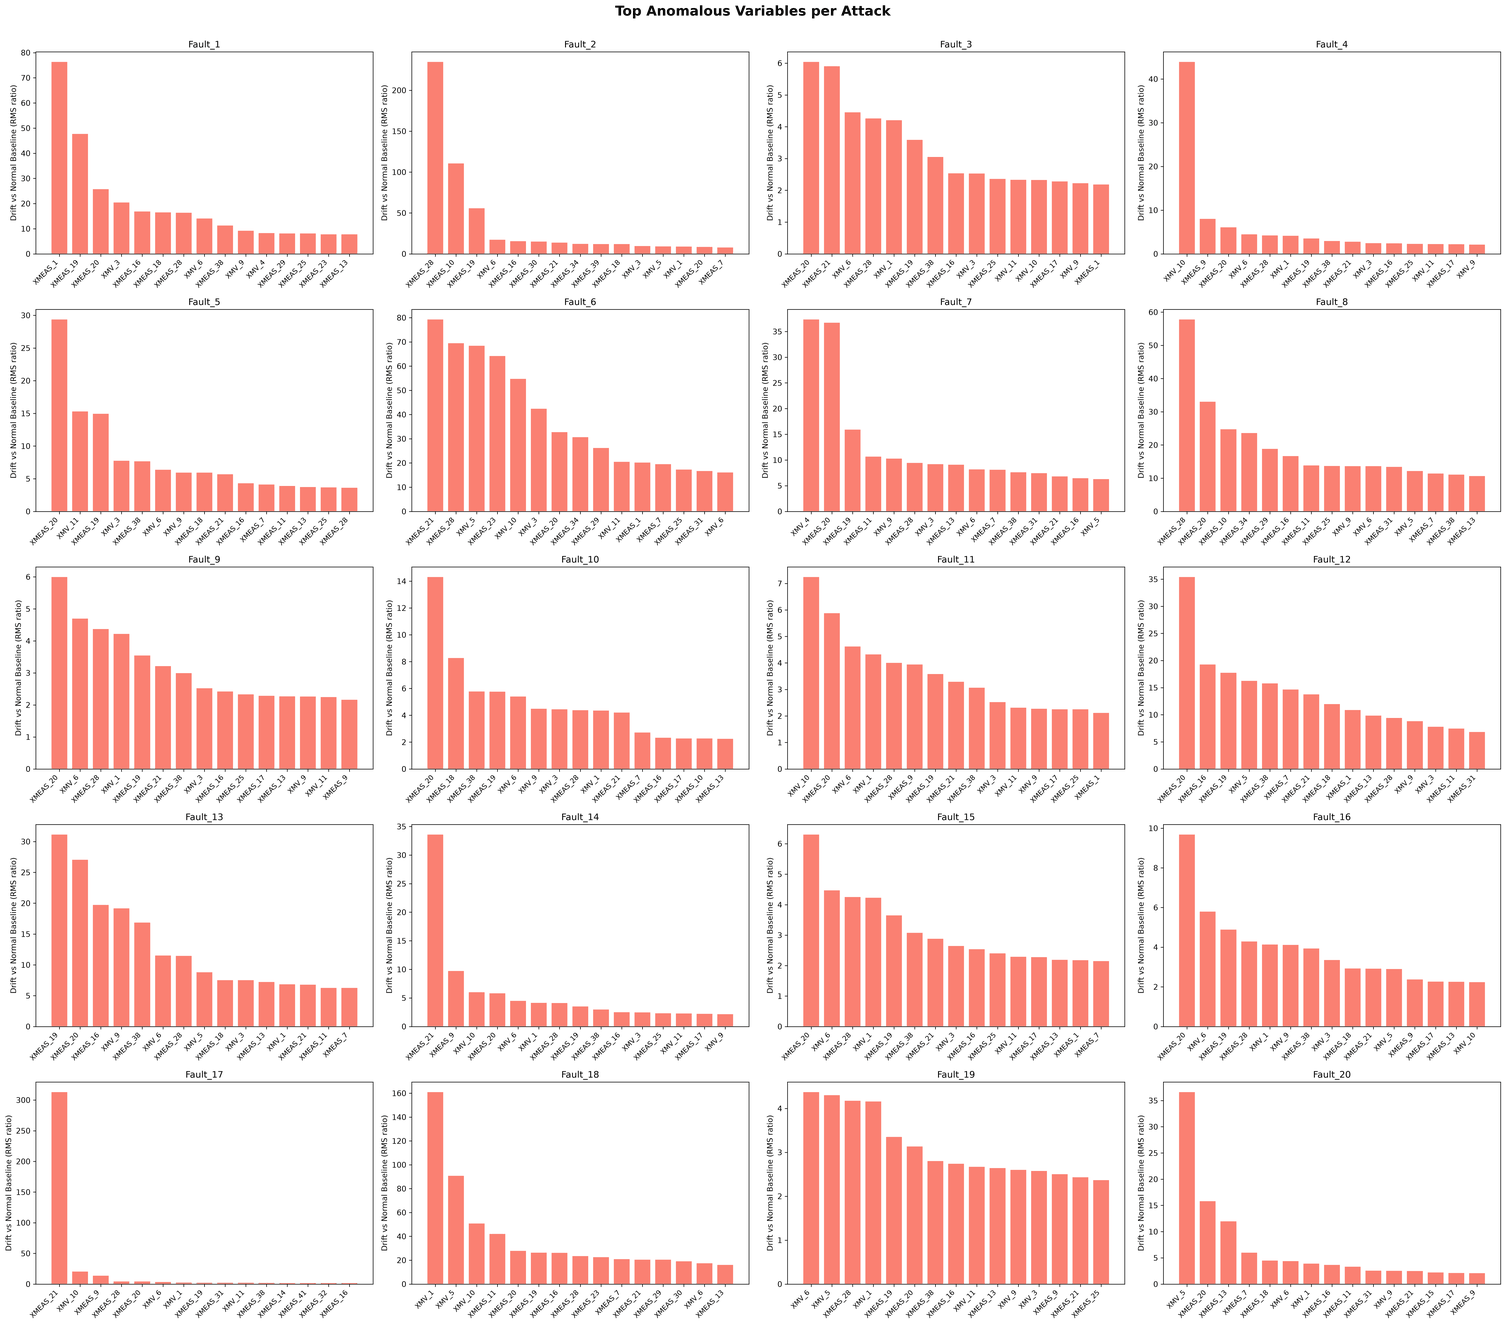
\includegraphics[width=0.85\textwidth,height=0.78\textheight,keepaspectratio]{camuv_industrial_linear_ridge.png}
  \caption[Attribution: CAM-UV, Industrial, linear/ridge]{Top attributed variables per attack class. CAM-UV, Industrial domain, linear/ridge.}
  \label{fig:camuv-industrial-linear-ridge}
\end{figure}

\begin{figure}[htbp]
  \centering
  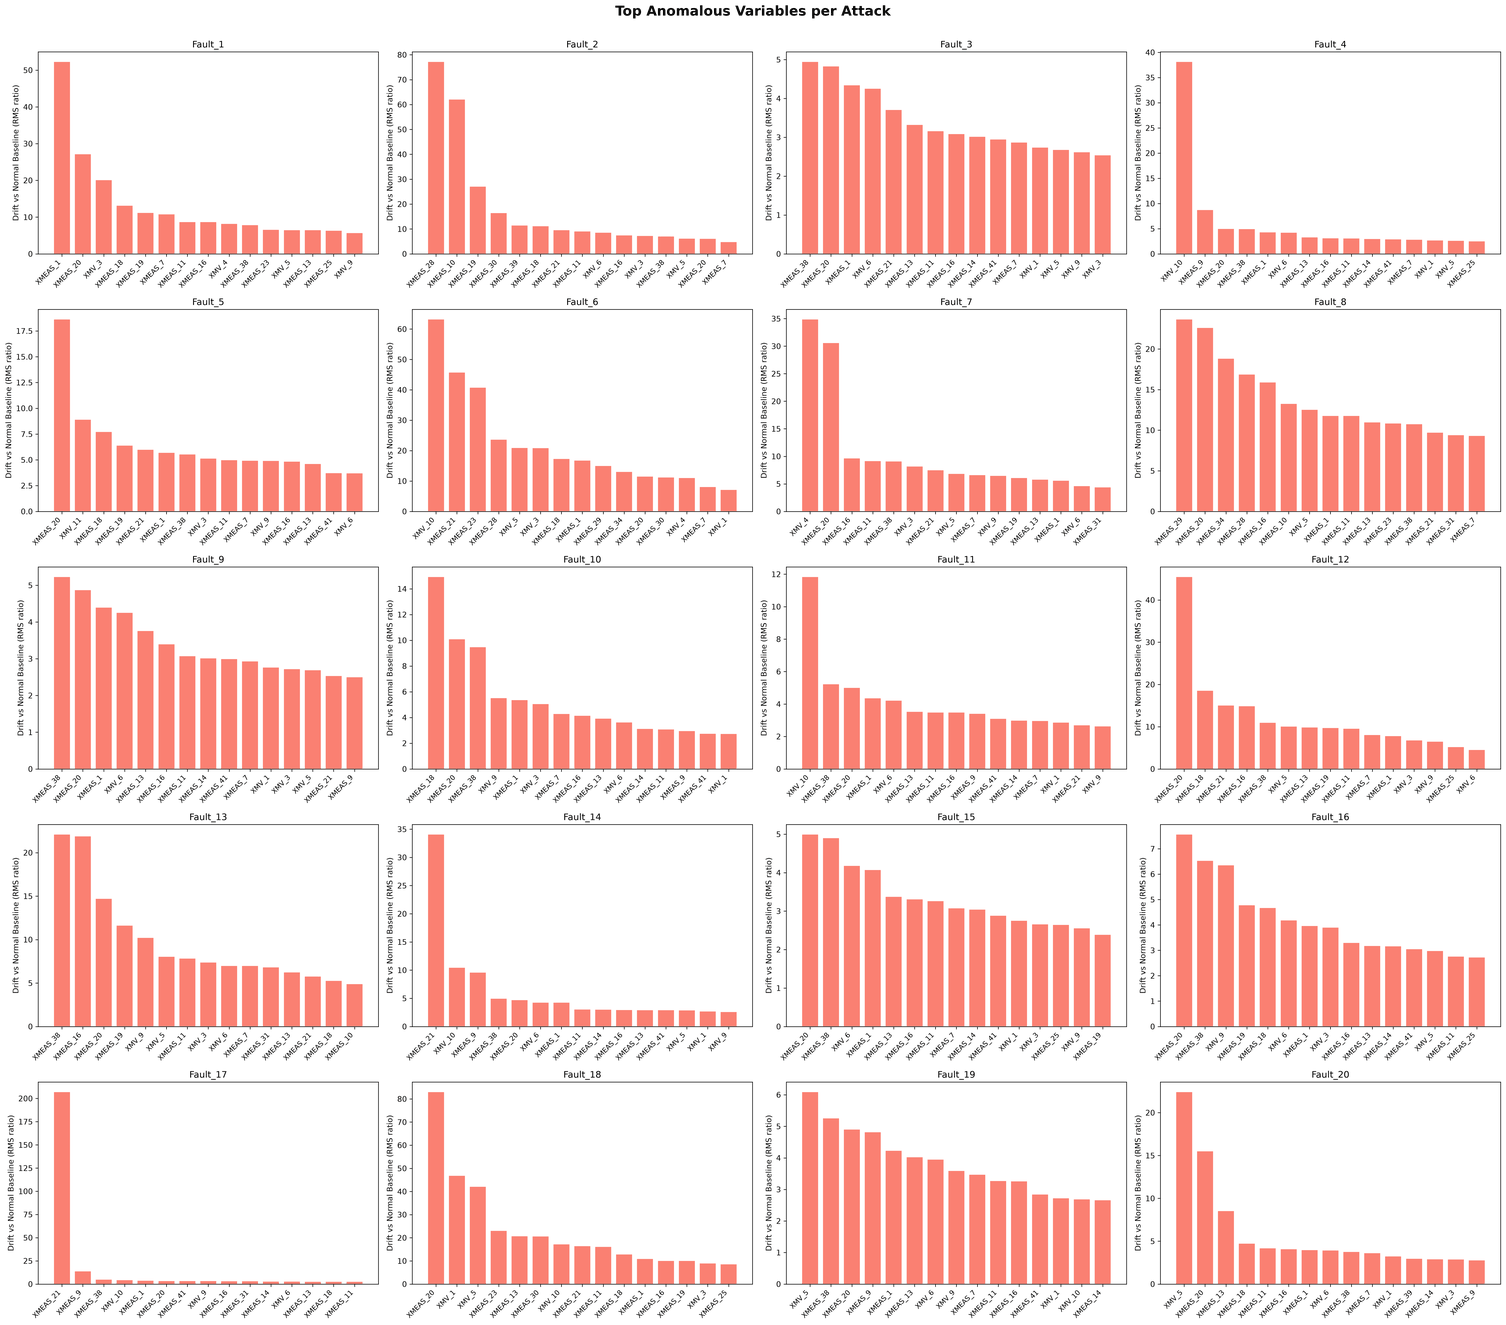
\includegraphics[width=0.85\textwidth,height=0.78\textheight,keepaspectratio]{camuv_industrial_polynomial_degree_3.png}
  \caption[Attribution: CAM-UV, Industrial, polynomial degree 3]{Top attributed variables per attack class. CAM-UV, Industrial domain, polynomial degree 3.}
  \label{fig:camuv-industrial-polynomial-degree-3}
\end{figure}

\begin{figure}[htbp]
  \centering
  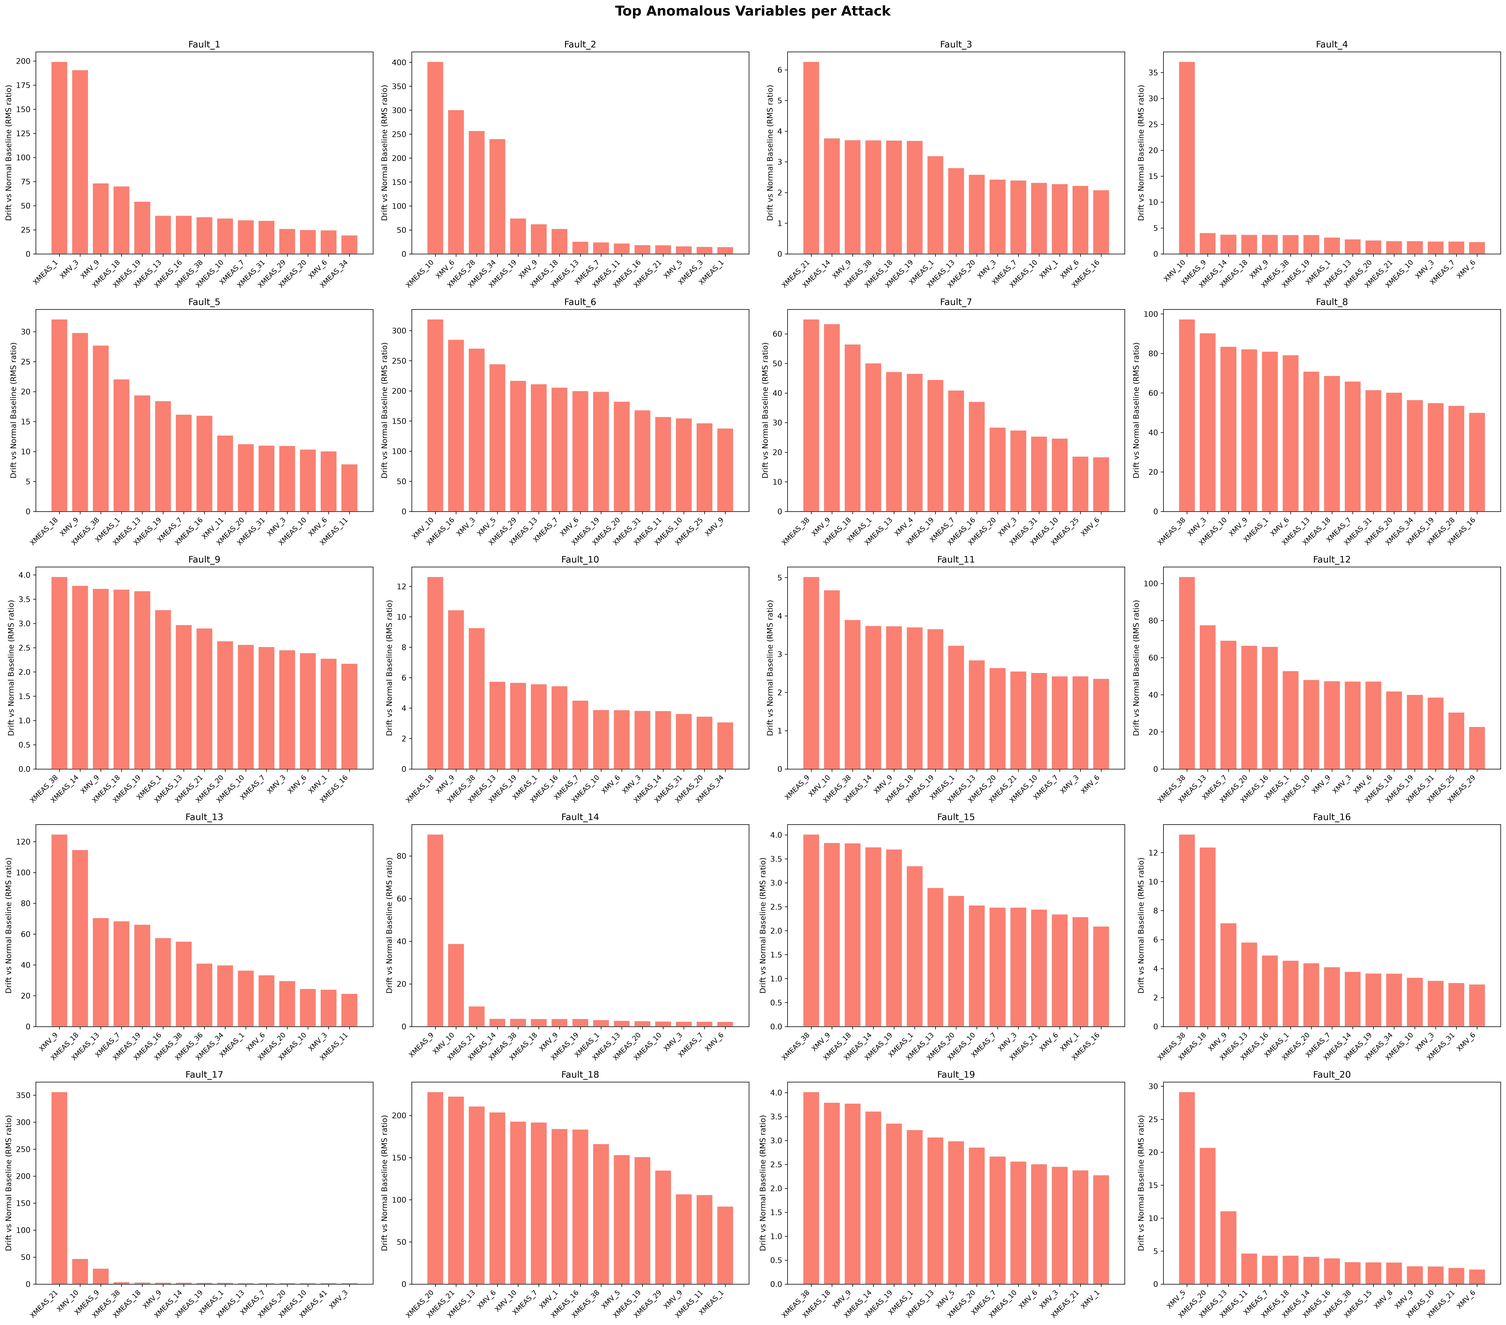
\includegraphics[width=0.85\textwidth,height=0.78\textheight,keepaspectratio]{camuv_industrial_rbf_ridge.png}
  \caption[Attribution: CAM-UV, Industrial, RBF + ridge]{Top attributed variables per attack class. CAM-UV, Industrial domain, RBF + ridge.}
  \label{fig:camuv-industrial-rbf-ridge}
\end{figure}

% Flush the per-configuration figures before the next section starts. They are
% full-page floats, so without this LaTeX defers them past two section breaks and
% prints them inside the baseline-attribution section they do not belong to.
\clearpage

\section{Paired AUC Comparisons}

Every comparison DeLong's test can reach, all 54 of them. The 54 it cannot reach are the pairs in which PCMCI faces one of the other two algorithms, and they are absent for the reason set out in Section~\ref{sec:uncertainty} rather than because they were not attempted.

% GENERATED by Thesis/tools/make_tables.py -- do not edit by hand.
% Every figure below is read from a CSV written by the pipelines.
{\footnotesize
\begin{longtable}{llrrrrr}
\caption[Every testable paired comparison, by DeLong's test]{Every testable paired comparison, by DeLong's test. $\Delta$ is AUC$_A$ minus AUC$_B$; $p$ is two-sided and is set in bold where it clears $\alpha = 0.05$. Pairs absent from this table are the 54 that share no sample set; the tool that writes this table also writes those, with the reason each one fails, to a companion CSV.}\label{tab:delong-full}\\
\toprule
A & B & AUC$_A$ & AUC$_B$ & $\Delta$ & $z$ & $p$ \\
\midrule
\endfirsthead
\toprule
A & B & AUC$_A$ & AUC$_B$ & $\Delta$ & $z$ & $p$ \\
\midrule
\endhead
\multicolumn{7}{l}{\textit{Healthcare (ECG)}} \\
CAM-UV Linear & CAM-UV Poly-3 & 0.7861 & 0.7691 & 0.0170 & 2.1897 & \textbf{0.028544} \\
CAM-UV Linear & CAM-UV RBF & 0.7861 & 0.7692 & 0.0169 & 2.5283 & \textbf{0.011461} \\
CAM-UV Linear & GES Linear & 0.7861 & 0.8114 & -0.0254 & -5.5553 & \textbf{0.000000} \\
CAM-UV Linear & GES Poly-3 & 0.7861 & 0.7867 & -0.0006 & -0.0853 & 0.932044 \\
CAM-UV Linear & GES RBF & 0.7861 & 0.7620 & 0.0241 & 3.4719 & \textbf{0.000517} \\
CAM-UV Poly-3 & CAM-UV RBF & 0.7691 & 0.7692 & -0.0001 & -0.0143 & 0.988601 \\
CAM-UV Poly-3 & GES Linear & 0.7691 & 0.8114 & -0.0423 & -5.2519 & \textbf{0.000000} \\
CAM-UV Poly-3 & GES Poly-3 & 0.7691 & 0.7867 & -0.0176 & -3.9817 & \textbf{0.000068} \\
CAM-UV Poly-3 & GES RBF & 0.7691 & 0.7620 & 0.0071 & 0.9705 & 0.331804 \\
CAM-UV RBF & GES Linear & 0.7692 & 0.8114 & -0.0422 & -6.1599 & \textbf{0.000000} \\
CAM-UV RBF & GES Poly-3 & 0.7692 & 0.7867 & -0.0175 & -2.6142 & \textbf{0.008944} \\
CAM-UV RBF & GES RBF & 0.7692 & 0.7620 & 0.0072 & 1.9235 & 0.054424 \\
\midrule
\multicolumn{7}{l}{\textit{Industrial (TEP)}} \\
CAM-UV Linear & CAM-UV Poly-3 & 0.8428 & 0.8212 & 0.0217 & 1.8245 & 0.068083 \\
CAM-UV Linear & CAM-UV RBF & 0.8428 & 0.8922 & -0.0494 & -6.3027 & \textbf{0.000000} \\
CAM-UV Linear & GES Linear & 0.8428 & 0.8407 & 0.0021 & 0.2920 & 0.770303 \\
CAM-UV Linear & GES Poly-3 & 0.8428 & 0.8849 & -0.0421 & -2.5705 & \textbf{0.010154} \\
CAM-UV Linear & GES RBF & 0.8428 & 0.8994 & -0.0565 & -7.1960 & \textbf{0.000000} \\
CAM-UV Poly-3 & CAM-UV RBF & 0.8212 & 0.8922 & -0.0711 & -4.8854 & \textbf{0.000001} \\
CAM-UV Poly-3 & GES Linear & 0.8212 & 0.8407 & -0.0195 & -1.3578 & 0.174527 \\
CAM-UV Poly-3 & GES Poly-3 & 0.8212 & 0.8849 & -0.0638 & -3.0470 & \textbf{0.002311} \\
CAM-UV Poly-3 & GES RBF & 0.8212 & 0.8994 & -0.0782 & -5.4280 & \textbf{0.000000} \\
CAM-UV RBF & GES Linear & 0.8922 & 0.8407 & 0.0515 & 8.0376 & \textbf{0.000000} \\
CAM-UV RBF & GES Poly-3 & 0.8922 & 0.8849 & 0.0073 & 0.5288 & 0.596928 \\
CAM-UV RBF & GES RBF & 0.8922 & 0.8994 & -0.0071 & -1.8047 & 0.071127 \\
\midrule
\multicolumn{7}{l}{\textit{Robotics (Pepper)}} \\
CAM-UV Linear & CAM-UV Poly-3 & 0.6497 & 0.6888 & -0.0391 & -2.4488 & \textbf{0.014334} \\
CAM-UV Linear & CAM-UV RBF & 0.6497 & 0.7818 & -0.1321 & -13.5592 & \textbf{0.000000} \\
CAM-UV Linear & GES Linear & 0.6497 & 0.5906 & 0.0591 & 4.8003 & \textbf{0.000002} \\
CAM-UV Linear & GES Poly-3 & 0.6497 & 0.6999 & -0.0502 & -3.0099 & \textbf{0.002614} \\
CAM-UV Linear & GES RBF & 0.6497 & 0.6516 & -0.0019 & -0.2423 & 0.808520 \\
CAM-UV Poly-3 & CAM-UV RBF & 0.6888 & 0.7818 & -0.0930 & -5.8060 & \textbf{0.000000} \\
CAM-UV Poly-3 & GES Linear & 0.6888 & 0.5906 & 0.0982 & 5.9541 & \textbf{0.000000} \\
CAM-UV Poly-3 & GES Poly-3 & 0.6888 & 0.6999 & -0.0111 & -1.0631 & 0.287753 \\
CAM-UV Poly-3 & GES RBF & 0.6888 & 0.6516 & 0.0372 & 2.5289 & \textbf{0.011443} \\
CAM-UV RBF & GES Linear & 0.7818 & 0.5906 & 0.1912 & 14.4240 & \textbf{0.000000} \\
CAM-UV RBF & GES Poly-3 & 0.7818 & 0.6999 & 0.0819 & 4.9478 & \textbf{0.000001} \\
CAM-UV RBF & GES RBF & 0.7818 & 0.6516 & 0.1302 & 15.3433 & \textbf{0.000000} \\
\midrule
\multicolumn{7}{l}{\textit{Healthcare (ECG)}} \\
GES Linear & GES Poly-3 & 0.8114 & 0.7867 & 0.0247 & 3.2587 & \textbf{0.001119} \\
GES Linear & GES RBF & 0.8114 & 0.7620 & 0.0494 & 7.4872 & \textbf{0.000000} \\
GES Poly-3 & GES RBF & 0.7867 & 0.7620 & 0.0247 & 3.6488 & \textbf{0.000263} \\
\midrule
\multicolumn{7}{l}{\textit{Industrial (TEP)}} \\
GES Linear & GES Poly-3 & 0.8407 & 0.8849 & -0.0442 & -2.7951 & \textbf{0.005188} \\
GES Linear & GES RBF & 0.8407 & 0.8994 & -0.0587 & -8.7444 & \textbf{0.000000} \\
GES Poly-3 & GES RBF & 0.8849 & 0.8994 & -0.0145 & -1.0202 & 0.307616 \\
\midrule
\multicolumn{7}{l}{\textit{Robotics (Pepper)}} \\
GES Linear & GES Poly-3 & 0.5906 & 0.6999 & -0.1093 & -8.2800 & \textbf{0.000000} \\
GES Linear & GES RBF & 0.5906 & 0.6516 & -0.0610 & -4.7679 & \textbf{0.000002} \\
GES Poly-3 & GES RBF & 0.6999 & 0.6516 & 0.0483 & 2.9049 & \textbf{0.003674} \\
\midrule
\multicolumn{7}{l}{\textit{Healthcare (ECG)}} \\
PCMCI Linear & PCMCI Poly-3 & 0.6181 & 0.5075 & 0.1106 & 13.2173 & \textbf{0.000000} \\
PCMCI Linear & PCMCI RBF & 0.6181 & 0.7147 & -0.0966 & -13.0939 & \textbf{0.000000} \\
PCMCI Poly-3 & PCMCI RBF & 0.5075 & 0.7147 & -0.2071 & -22.9203 & \textbf{0.000000} \\
\midrule
\multicolumn{7}{l}{\textit{Industrial (TEP)}} \\
PCMCI Linear & PCMCI Poly-3 & 0.8860 & 0.9151 & -0.0291 & -9.7046 & \textbf{0.000000} \\
PCMCI Linear & PCMCI RBF & 0.8860 & 0.8495 & 0.0365 & 8.1254 & \textbf{0.000000} \\
PCMCI Poly-3 & PCMCI RBF & 0.9151 & 0.8495 & 0.0656 & 17.5271 & \textbf{0.000000} \\
\midrule
\multicolumn{7}{l}{\textit{Robotics (Pepper)}} \\
PCMCI Linear & PCMCI Poly-3 & 0.7825 & 0.8053 & -0.0228 & -0.8914 & 0.372739 \\
PCMCI Linear & PCMCI RBF & 0.7825 & 0.8752 & -0.0927 & -4.3958 & \textbf{0.000011} \\
PCMCI Poly-3 & PCMCI RBF & 0.8053 & 0.8752 & -0.0699 & -3.9526 & \textbf{0.000077} \\
\bottomrule
\end{longtable}}


\section{Baseline Attribution Plots}

Chapter~\ref{ch:results} reports the SHAP attributions through the relevance and consistency scores computed over them, and leaves the attributions themselves here. Table~\ref{tab:shap} gives the top-ranked variable each architecture returns for the three robotics attack classes, on the same faults as the causal attributions of Table~\ref{tab:attributions}.

% GENERATED by Thesis/tools/make_tables.py -- do not edit by hand.
% Every figure below is read from a CSV written by the pipelines.
\begin{table}[htbp]
\centering
\small
\caption[Post-hoc SHAP attribution over the neural autoencoders]{Post-hoc SHAP attribution over the neural autoencoders, on the same three robotics attack classes as the causal attributions in Table~\ref{tab:attributions}. SHAP recovers a tablet sensor for the LED attack in two of three architectures; the intrinsic causal attribution recovers one in nine of nine.}
\label{tab:shap}
\begin{tabular}{llll}
\toprule
Architecture & LedsControl & JointControl & WheelsControl \\
\midrule
LSTM & LedFaceBR5 & RShoulderPitch & WheelBSpeed \\
TCN & \textbf{TabletTouchX} & RShoulderPitch & WheelBSpeed \\
Transformer & \textbf{TabletTouchX} & RShoulderPitch & WheelBSpeed \\
\bottomrule
\end{tabular}
\end{table}


SHAP returns a different top variable depending on which architecture it is asked to explain, recovering a tablet sensor for the TCN and the Transformer on the LED fault and failing on the LSTM. The drift-based attribution returns the same answer across three algorithms with three different graphs and two different variable sets, two of which do not model the attacked sensors at all. Figures~\ref{fig:shap-lstm-leds} to~\ref{fig:shap-transformer-leds} are the three \texttt{LedsControl} panels behind that row, which is where the contrast with the causal attribution is sharpest.

\begin{figure}[htbp]
  \centering
  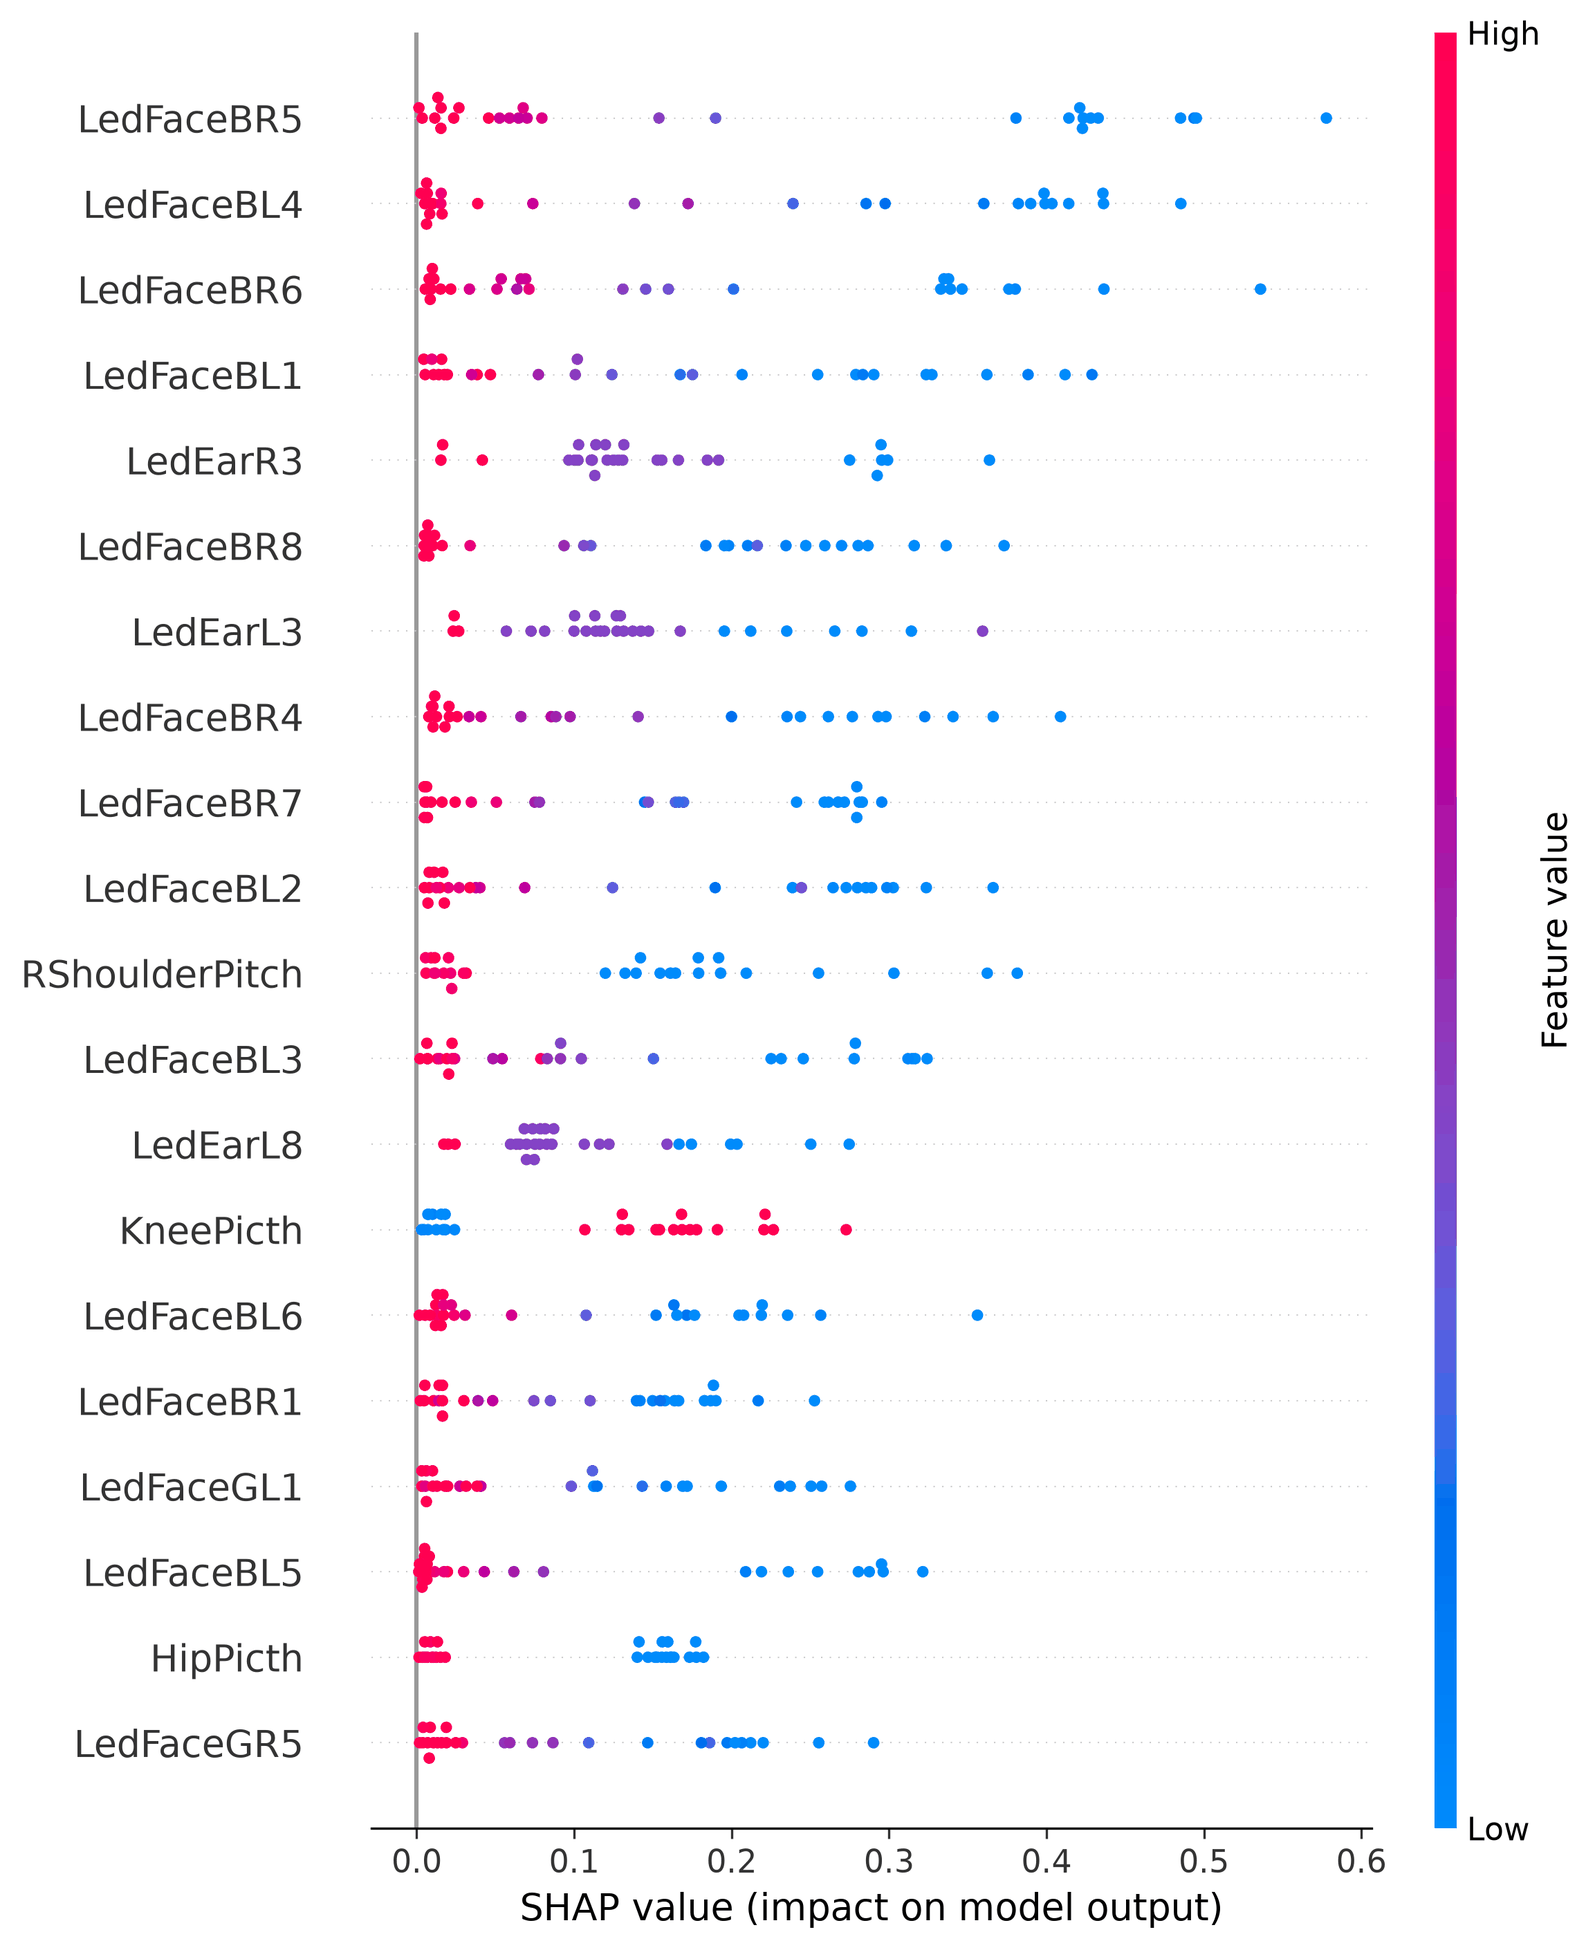
\includegraphics[width=0.9\textwidth]{baseline_shap_lstm_autoencoder_ledscontrol.png}
  \caption{SHAP attribution for the LSTM autoencoder on the \texttt{LedsControl} fault.}
  \label{fig:shap-lstm-leds}
\end{figure}

\begin{figure}[htbp]
  \centering
  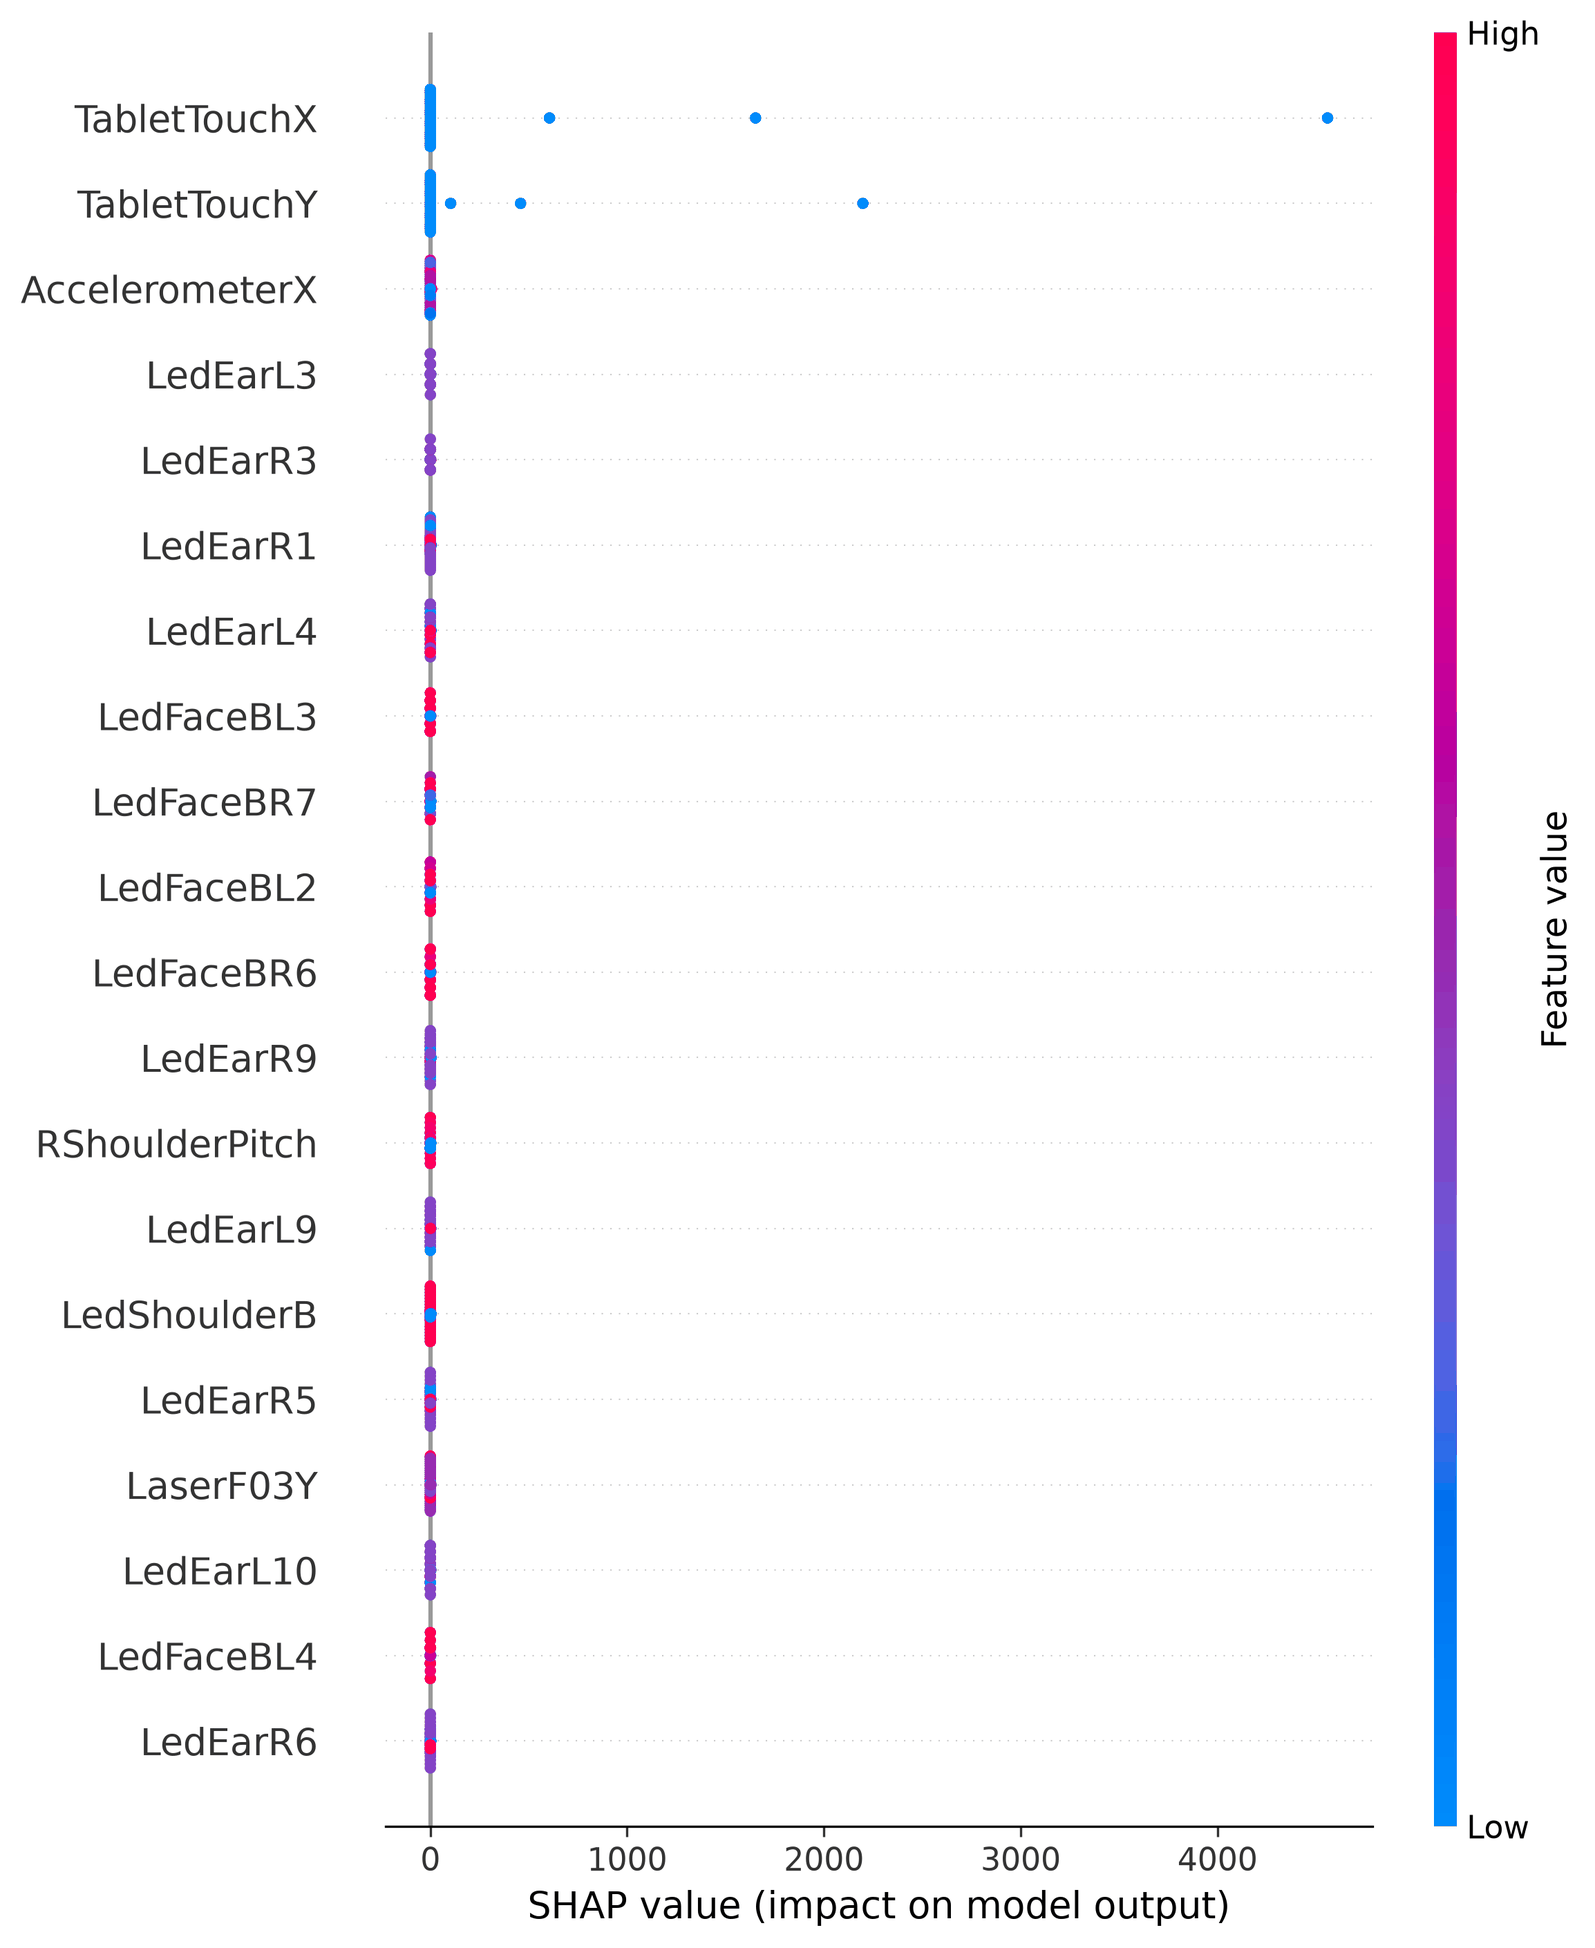
\includegraphics[width=0.9\textwidth]{baseline_shap_tcn_autoencoder_ledscontrol.png}
  \caption{SHAP attribution for the TCN autoencoder on the \texttt{LedsControl} fault.}
  \label{fig:shap-tcn-leds}
\end{figure}

\begin{figure}[htbp]
  \centering
  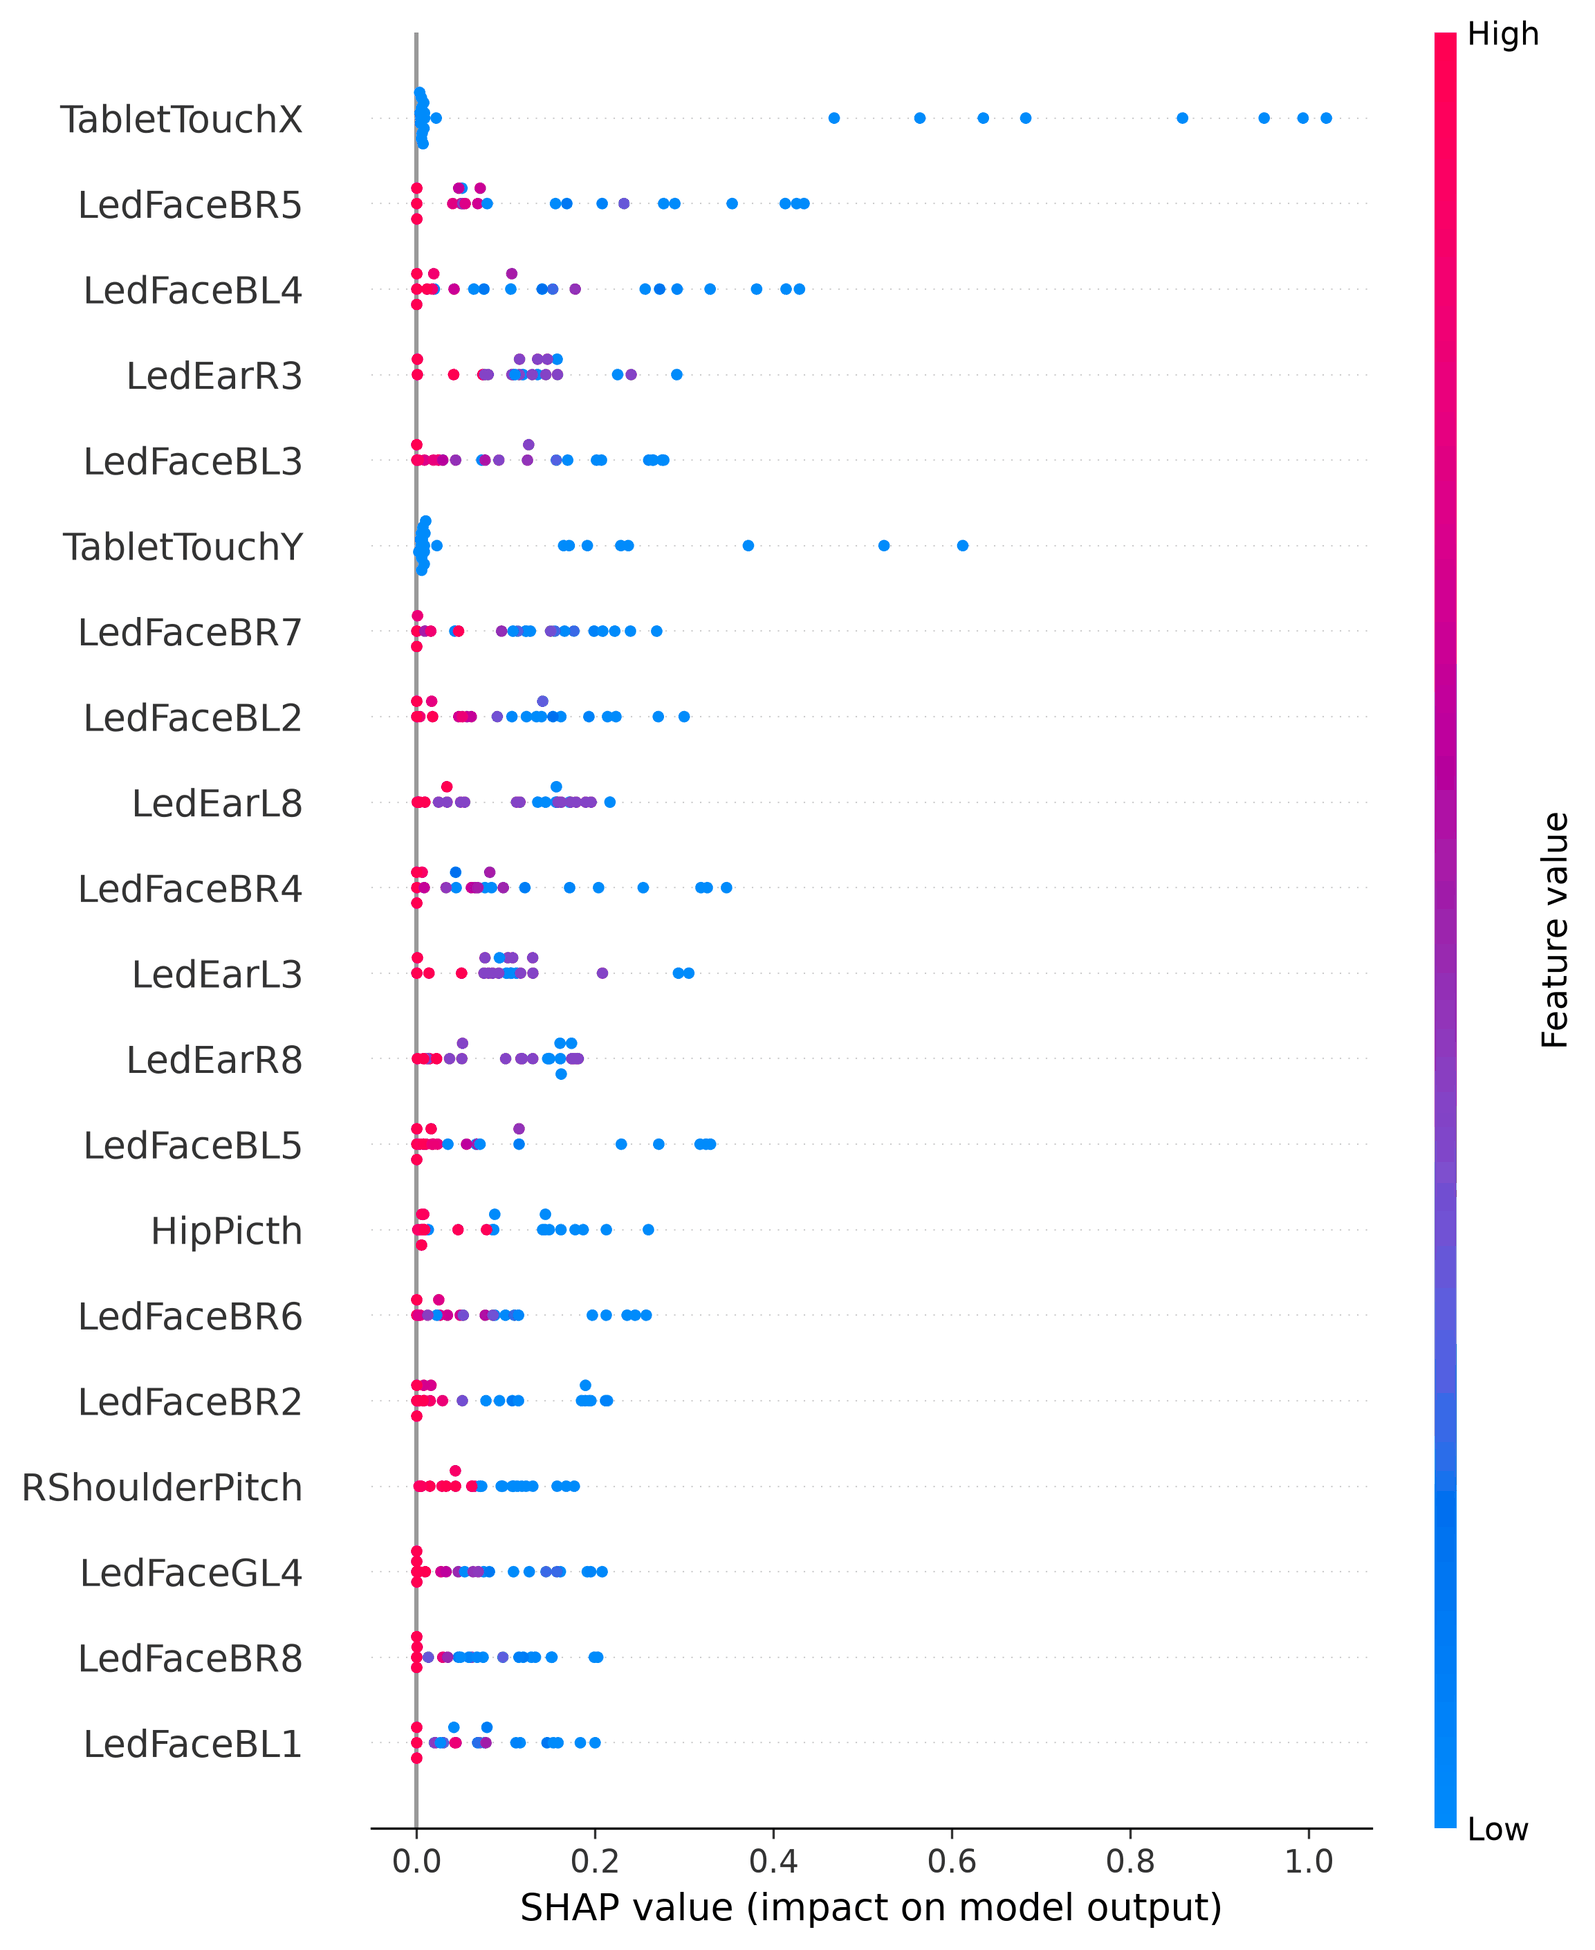
\includegraphics[width=0.9\textwidth]{baseline_shap_transformer_autoencoder_ledscontrol.png}
  \caption{SHAP attribution for the Transformer autoencoder on the \texttt{LedsControl} fault.}
  \label{fig:shap-transformer-leds}
\end{figure}

The other two robotics faults follow, as Figures~\ref{fig:baseline-shap-lstm-autoencoder-jointcontrol} to~\ref{fig:baseline-shap-transformer-autoencoder-wheelscontrol}. The \texttt{JointControl} figures are the ones to read against Table~\ref{tab:deviation}: all three architectures return \texttt{RShoulderPitch}, which is the variable with the largest standardised deviation in the system and not the joint temperature the documented requirement names.

\begin{figure}[htbp]
  \centering
  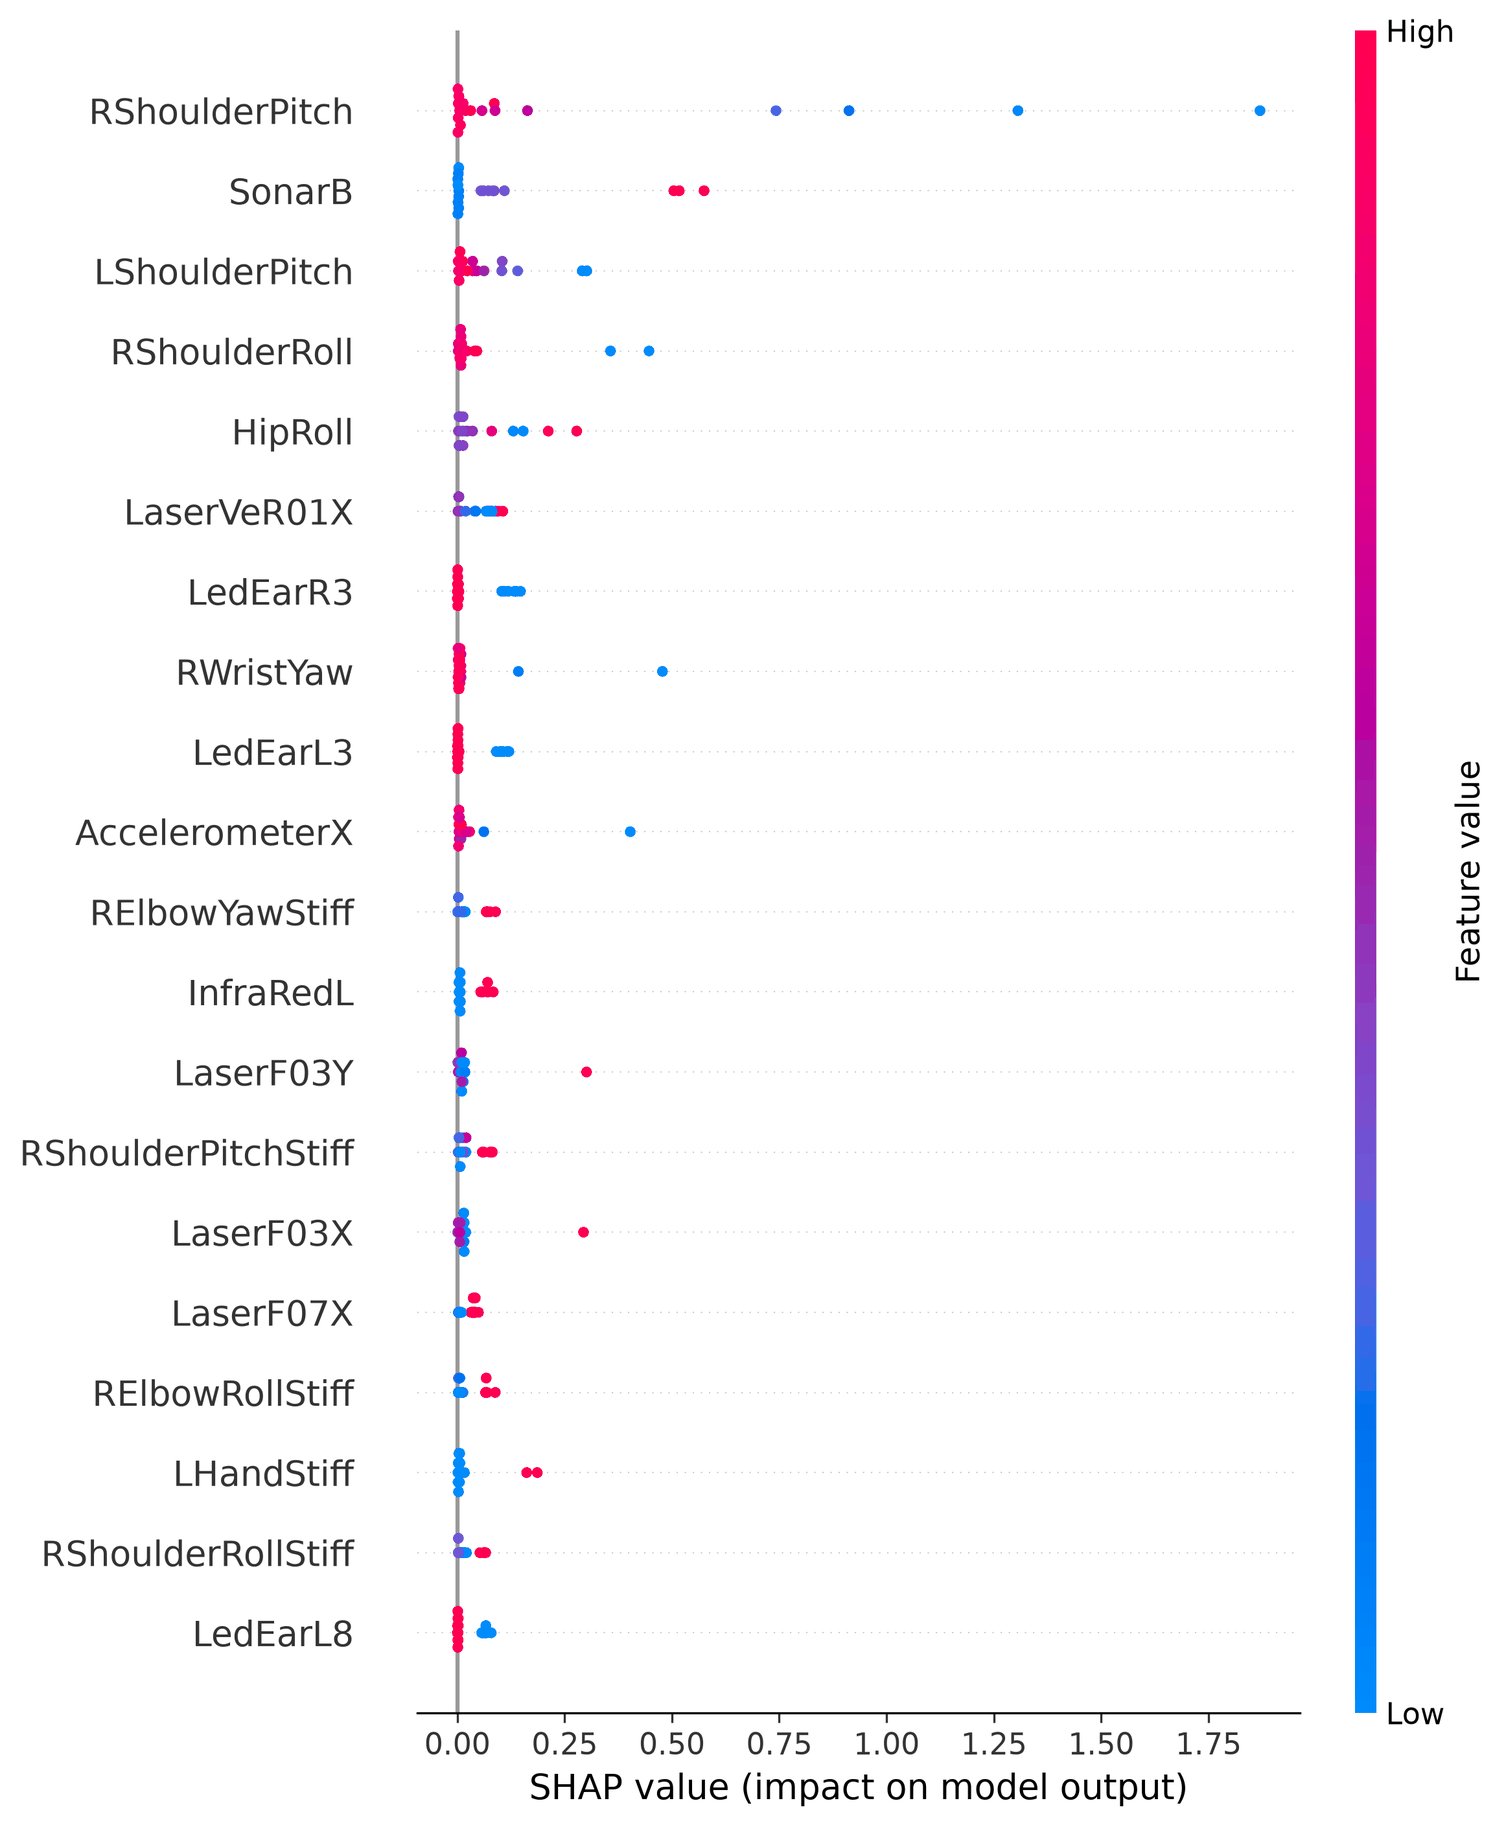
\includegraphics[width=0.85\textwidth,height=0.78\textheight,keepaspectratio]{baseline_shap_lstm_autoencoder_jointcontrol.png}
  \caption[SHAP: LSTM, JointControl]{SHAP attribution for the LSTM autoencoder on the \texttt{JointControl} fault.}
  \label{fig:baseline-shap-lstm-autoencoder-jointcontrol}
\end{figure}

\begin{figure}[htbp]
  \centering
  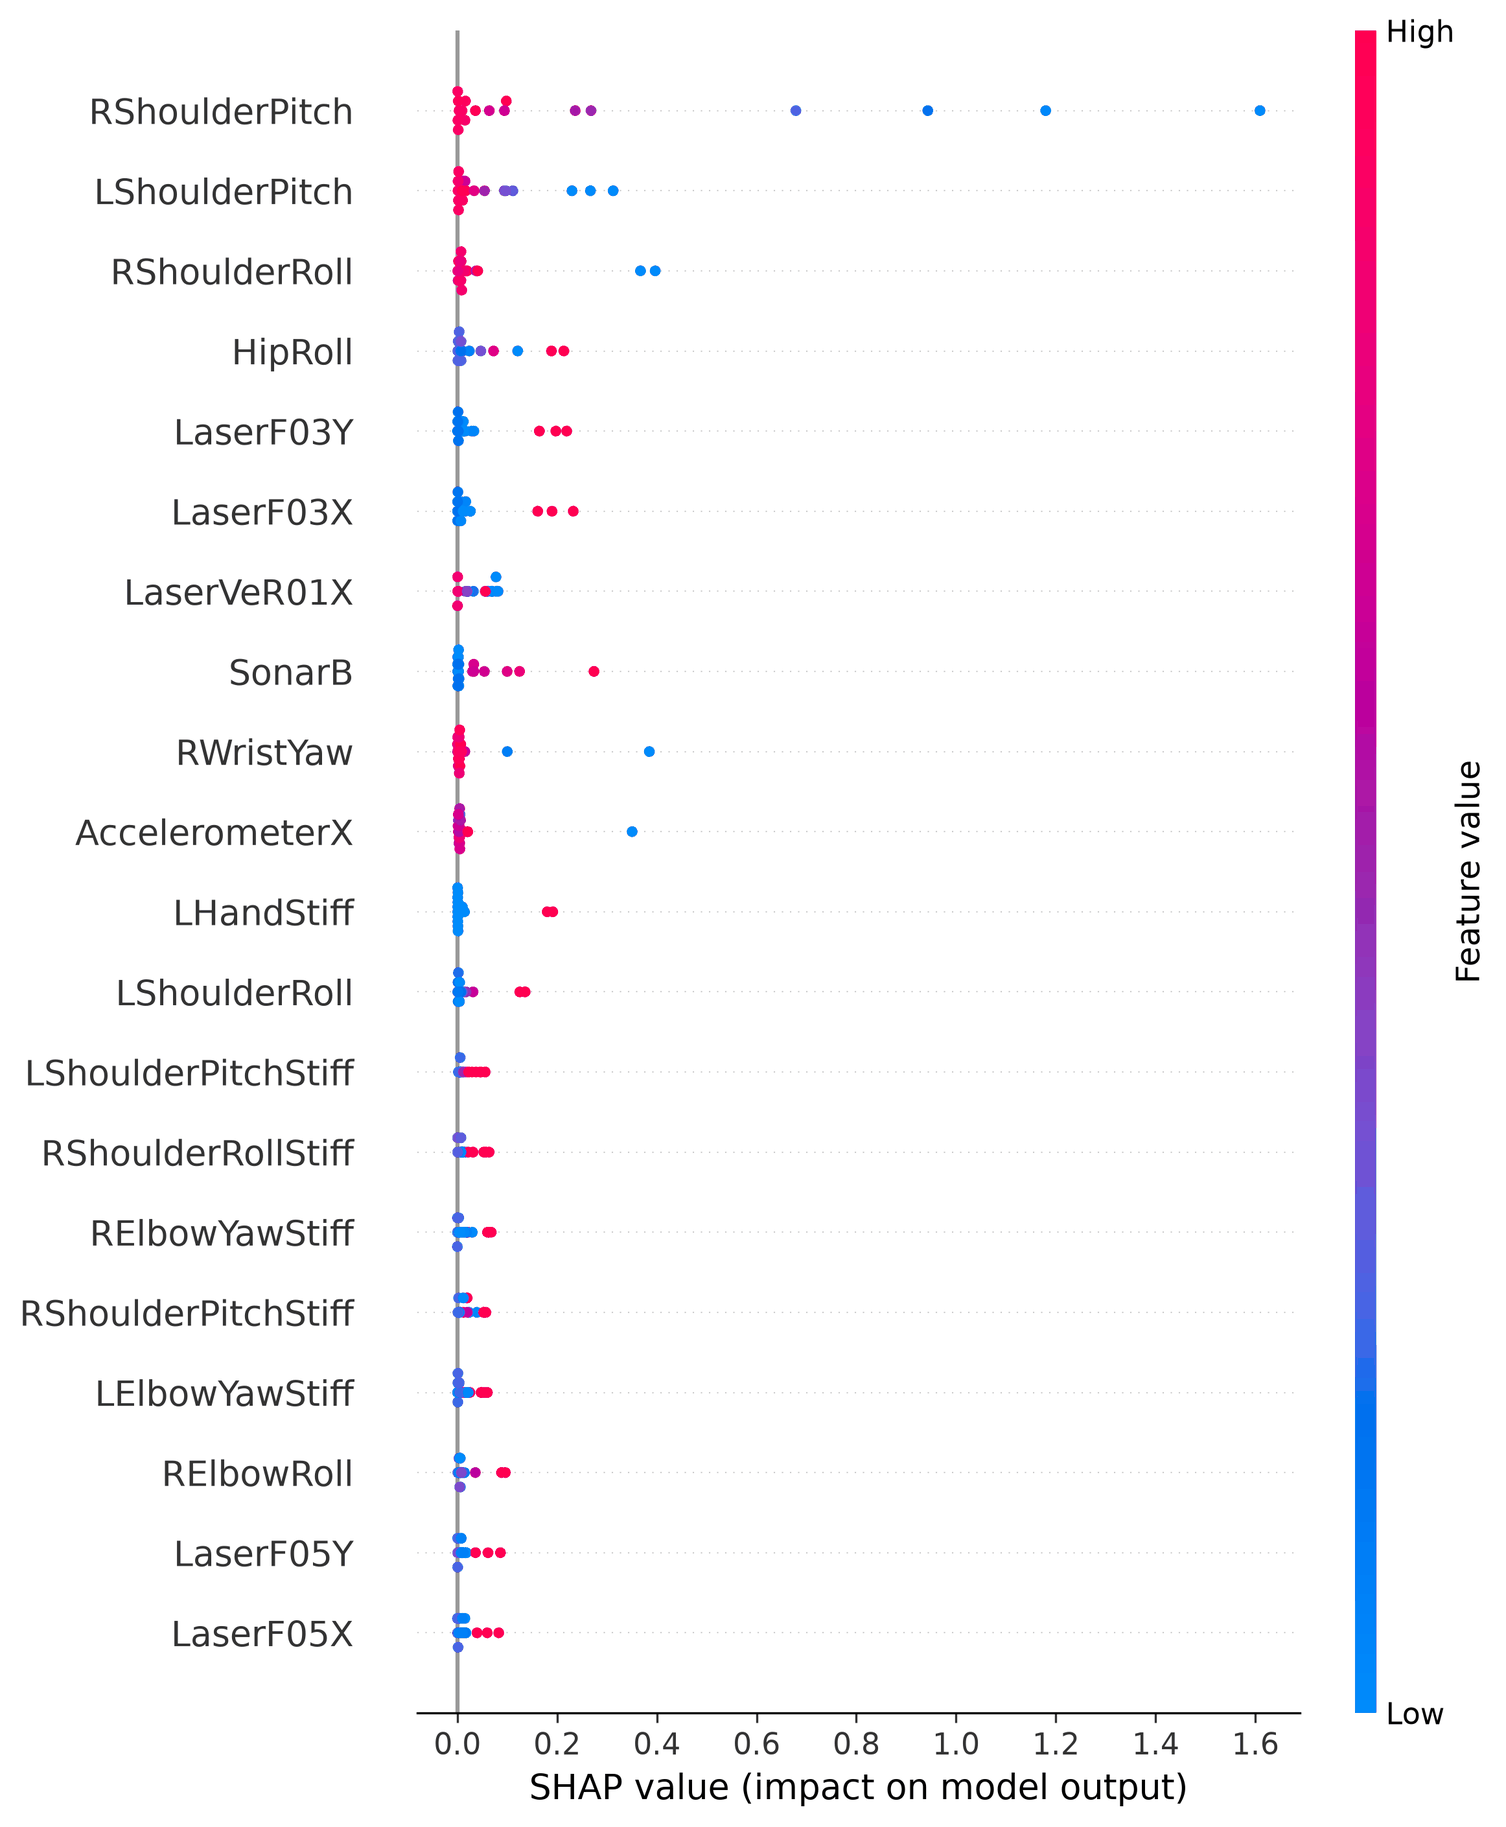
\includegraphics[width=0.85\textwidth,height=0.78\textheight,keepaspectratio]{baseline_shap_tcn_autoencoder_jointcontrol.png}
  \caption[SHAP: TCN, JointControl]{SHAP attribution for the TCN autoencoder on the \texttt{JointControl} fault.}
  \label{fig:baseline-shap-tcn-autoencoder-jointcontrol}
\end{figure}

\begin{figure}[htbp]
  \centering
  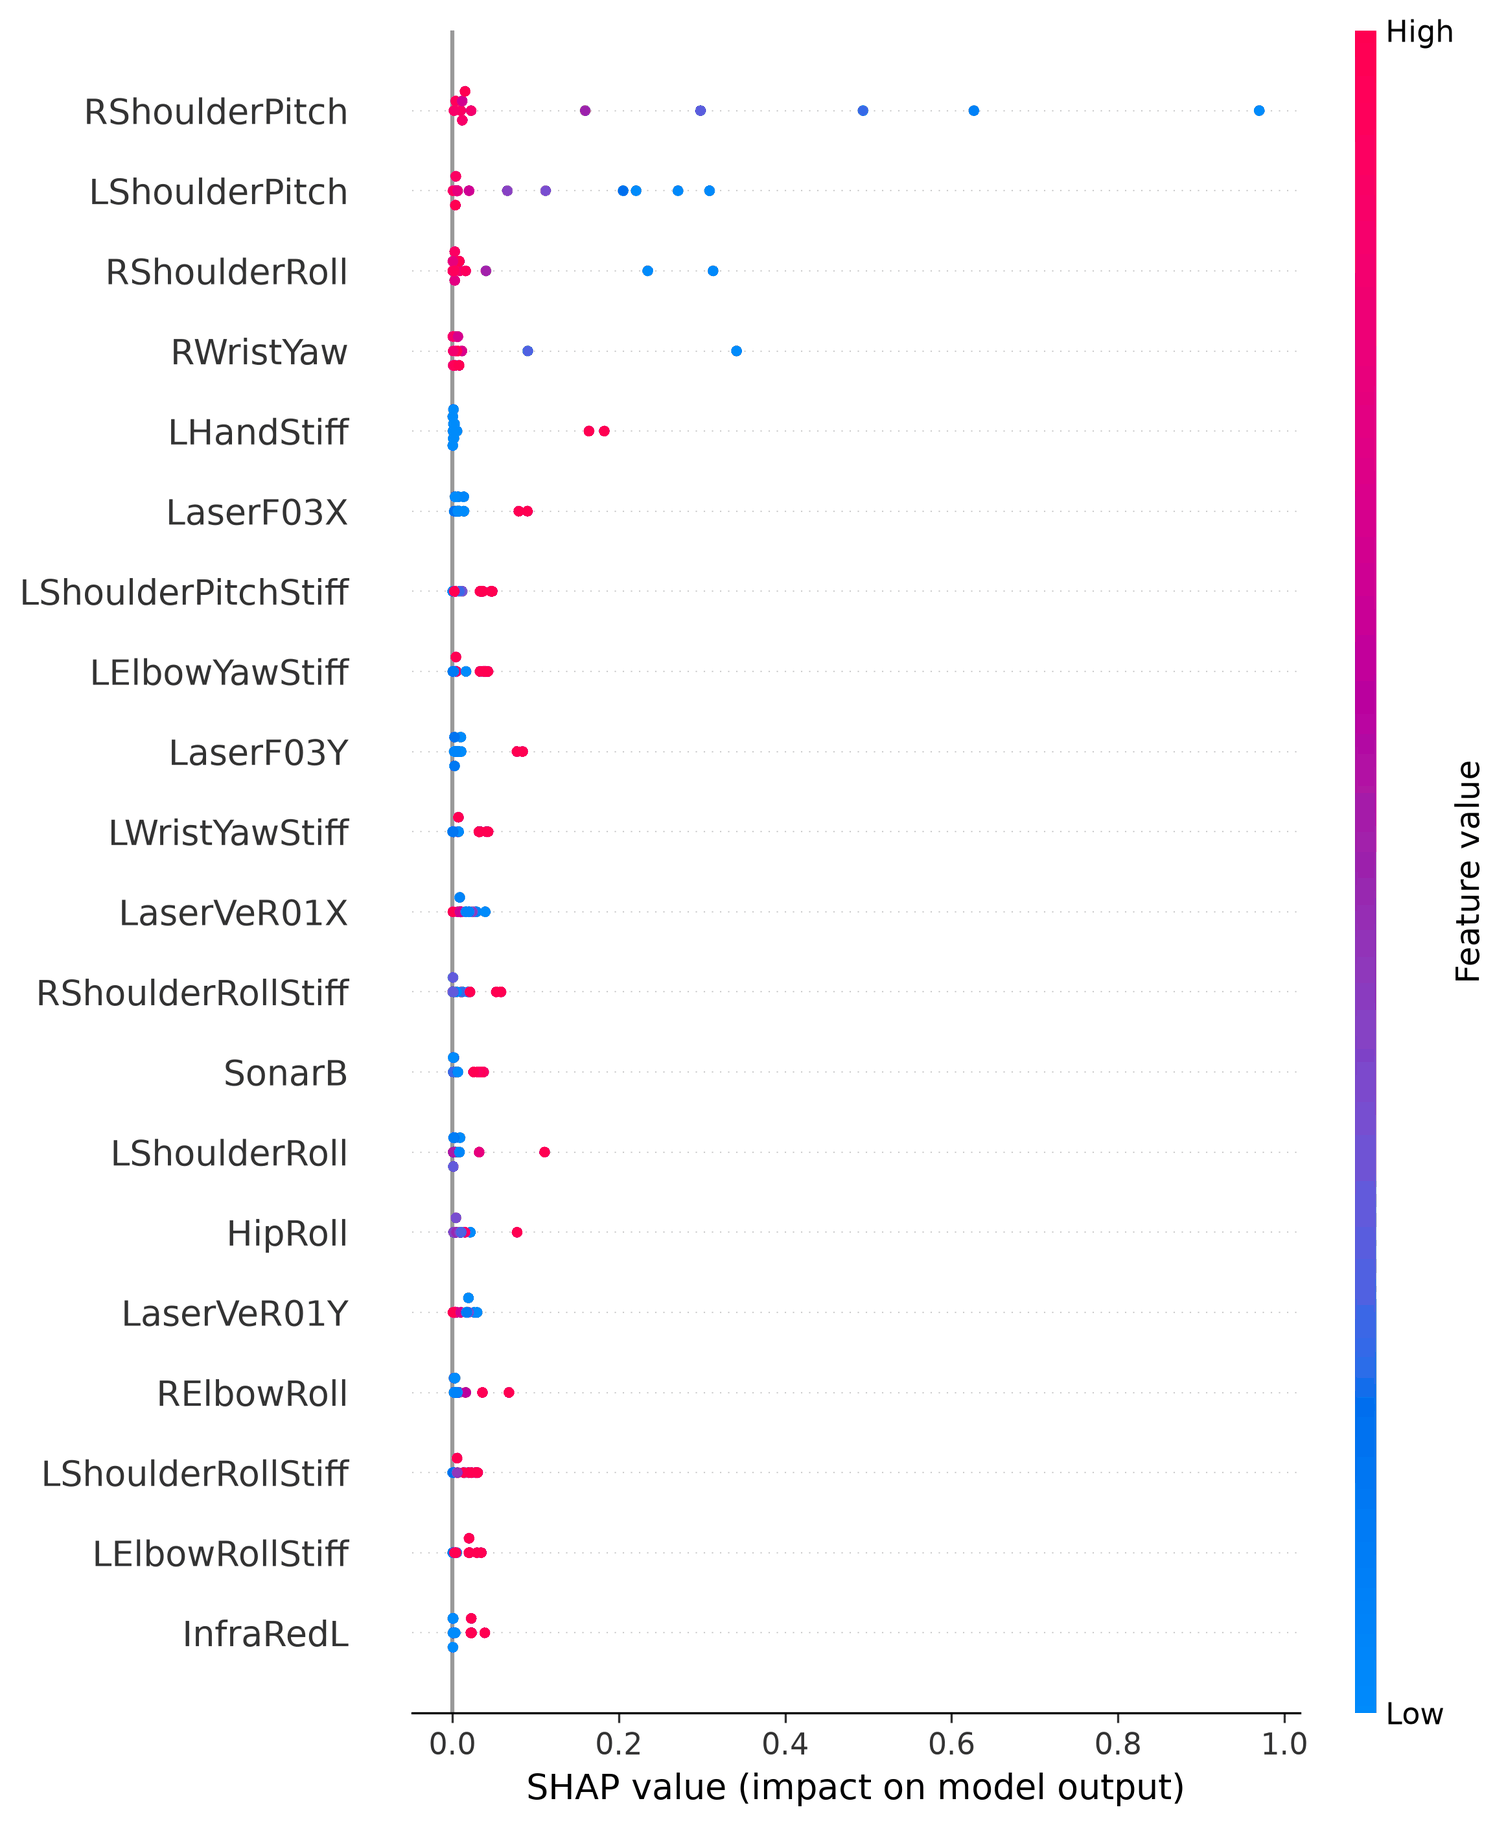
\includegraphics[width=0.85\textwidth,height=0.78\textheight,keepaspectratio]{baseline_shap_transformer_autoencoder_jointcontrol.png}
  \caption[SHAP: Transformer, JointControl]{SHAP attribution for the Transformer autoencoder on the \texttt{JointControl} fault.}
  \label{fig:baseline-shap-transformer-autoencoder-jointcontrol}
\end{figure}

\begin{figure}[htbp]
  \centering
  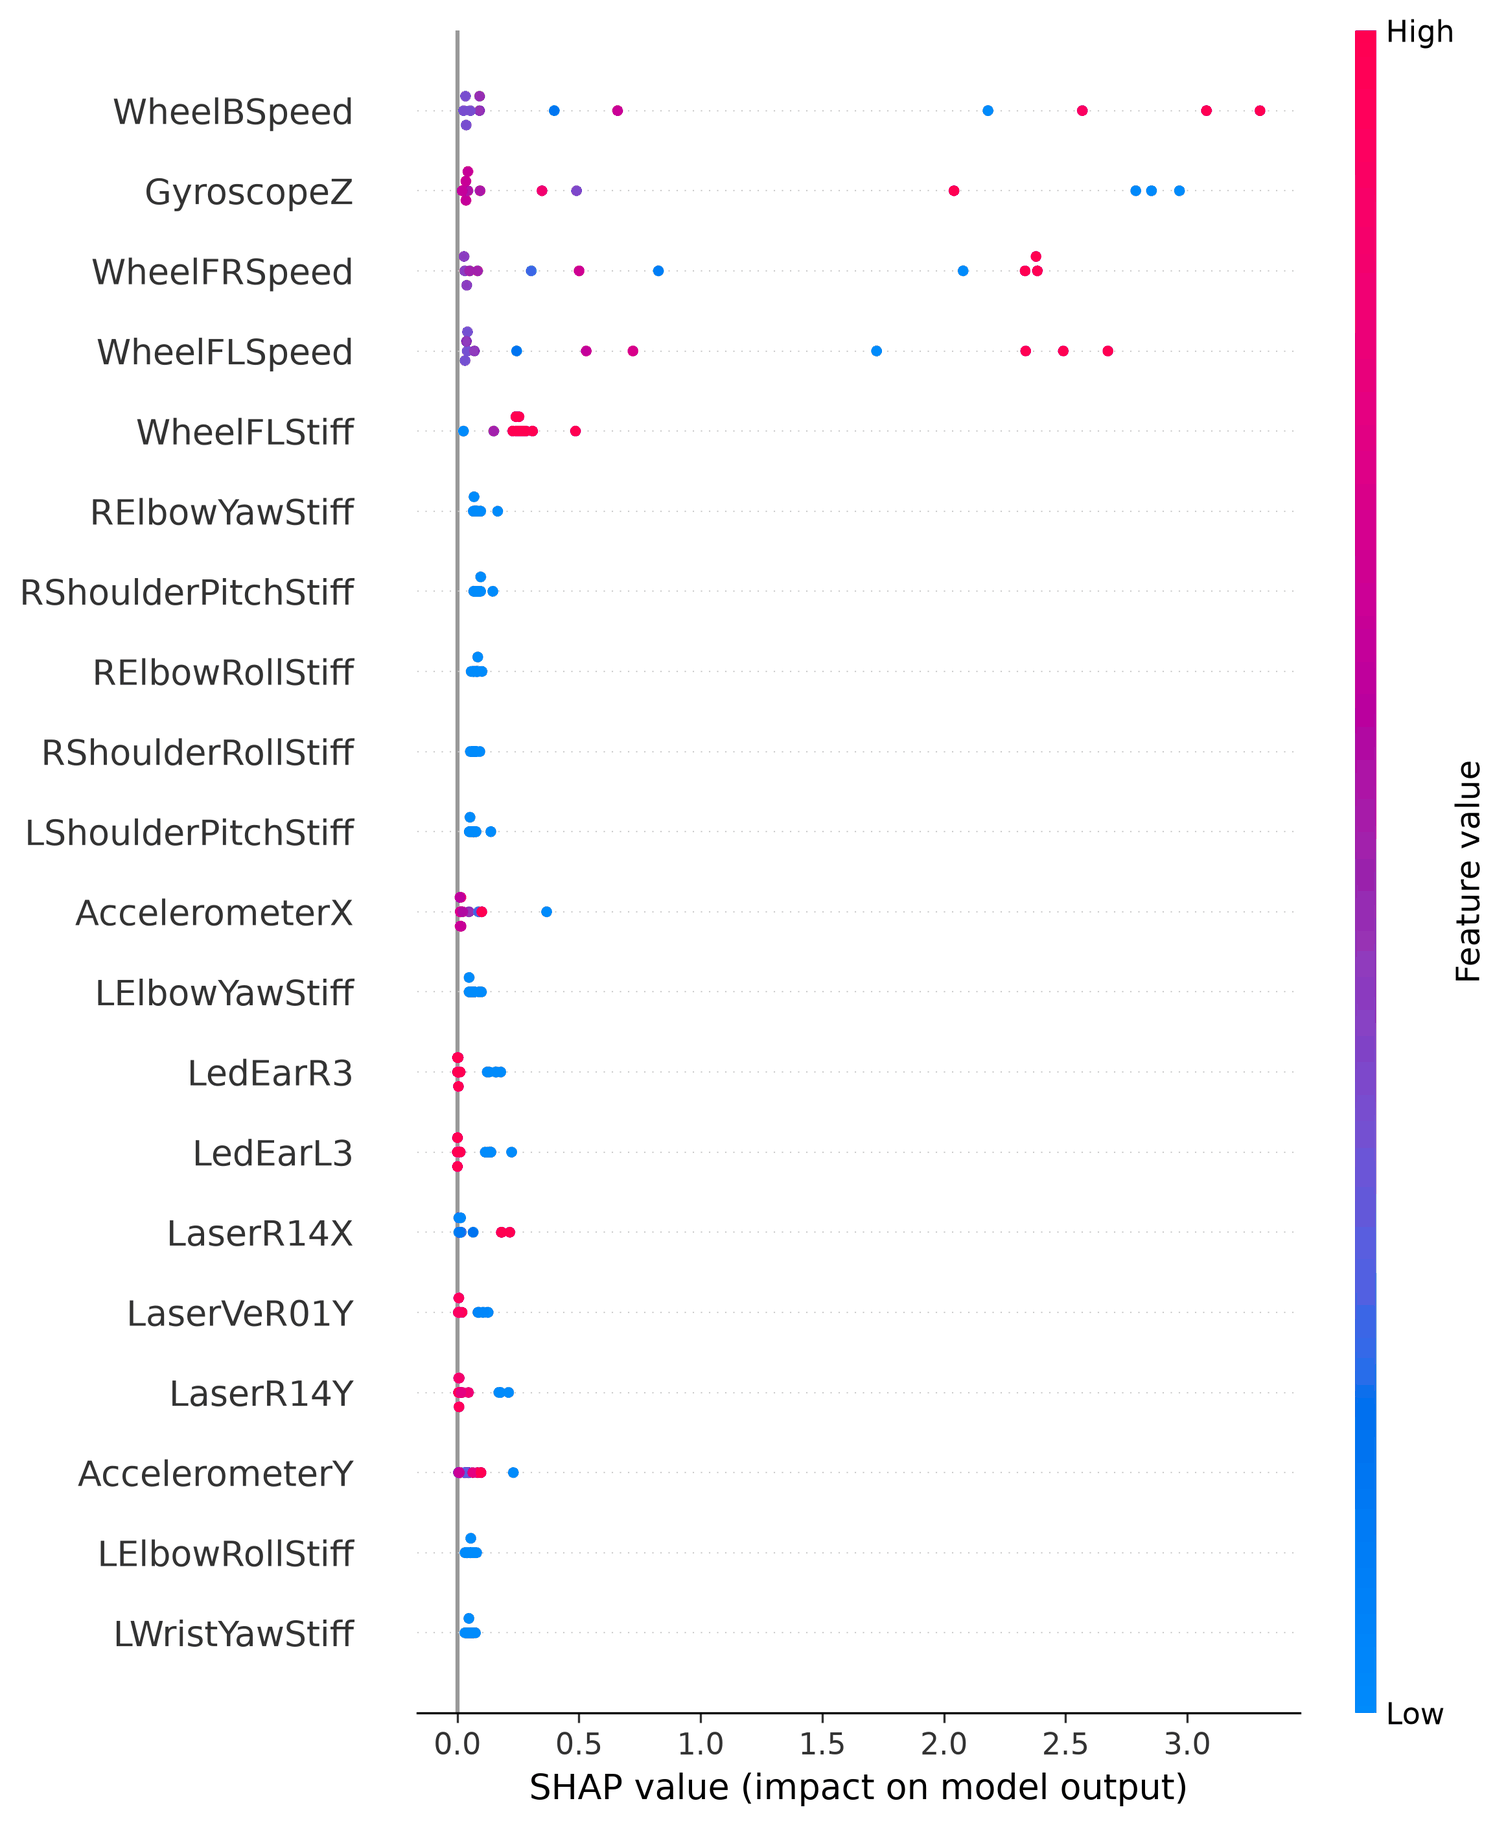
\includegraphics[width=0.85\textwidth,height=0.78\textheight,keepaspectratio]{baseline_shap_lstm_autoencoder_wheelscontrol.png}
  \caption[SHAP: LSTM, WheelsControl]{SHAP attribution for the LSTM autoencoder on the \texttt{WheelsControl} fault.}
  \label{fig:baseline-shap-lstm-autoencoder-wheelscontrol}
\end{figure}

\begin{figure}[htbp]
  \centering
  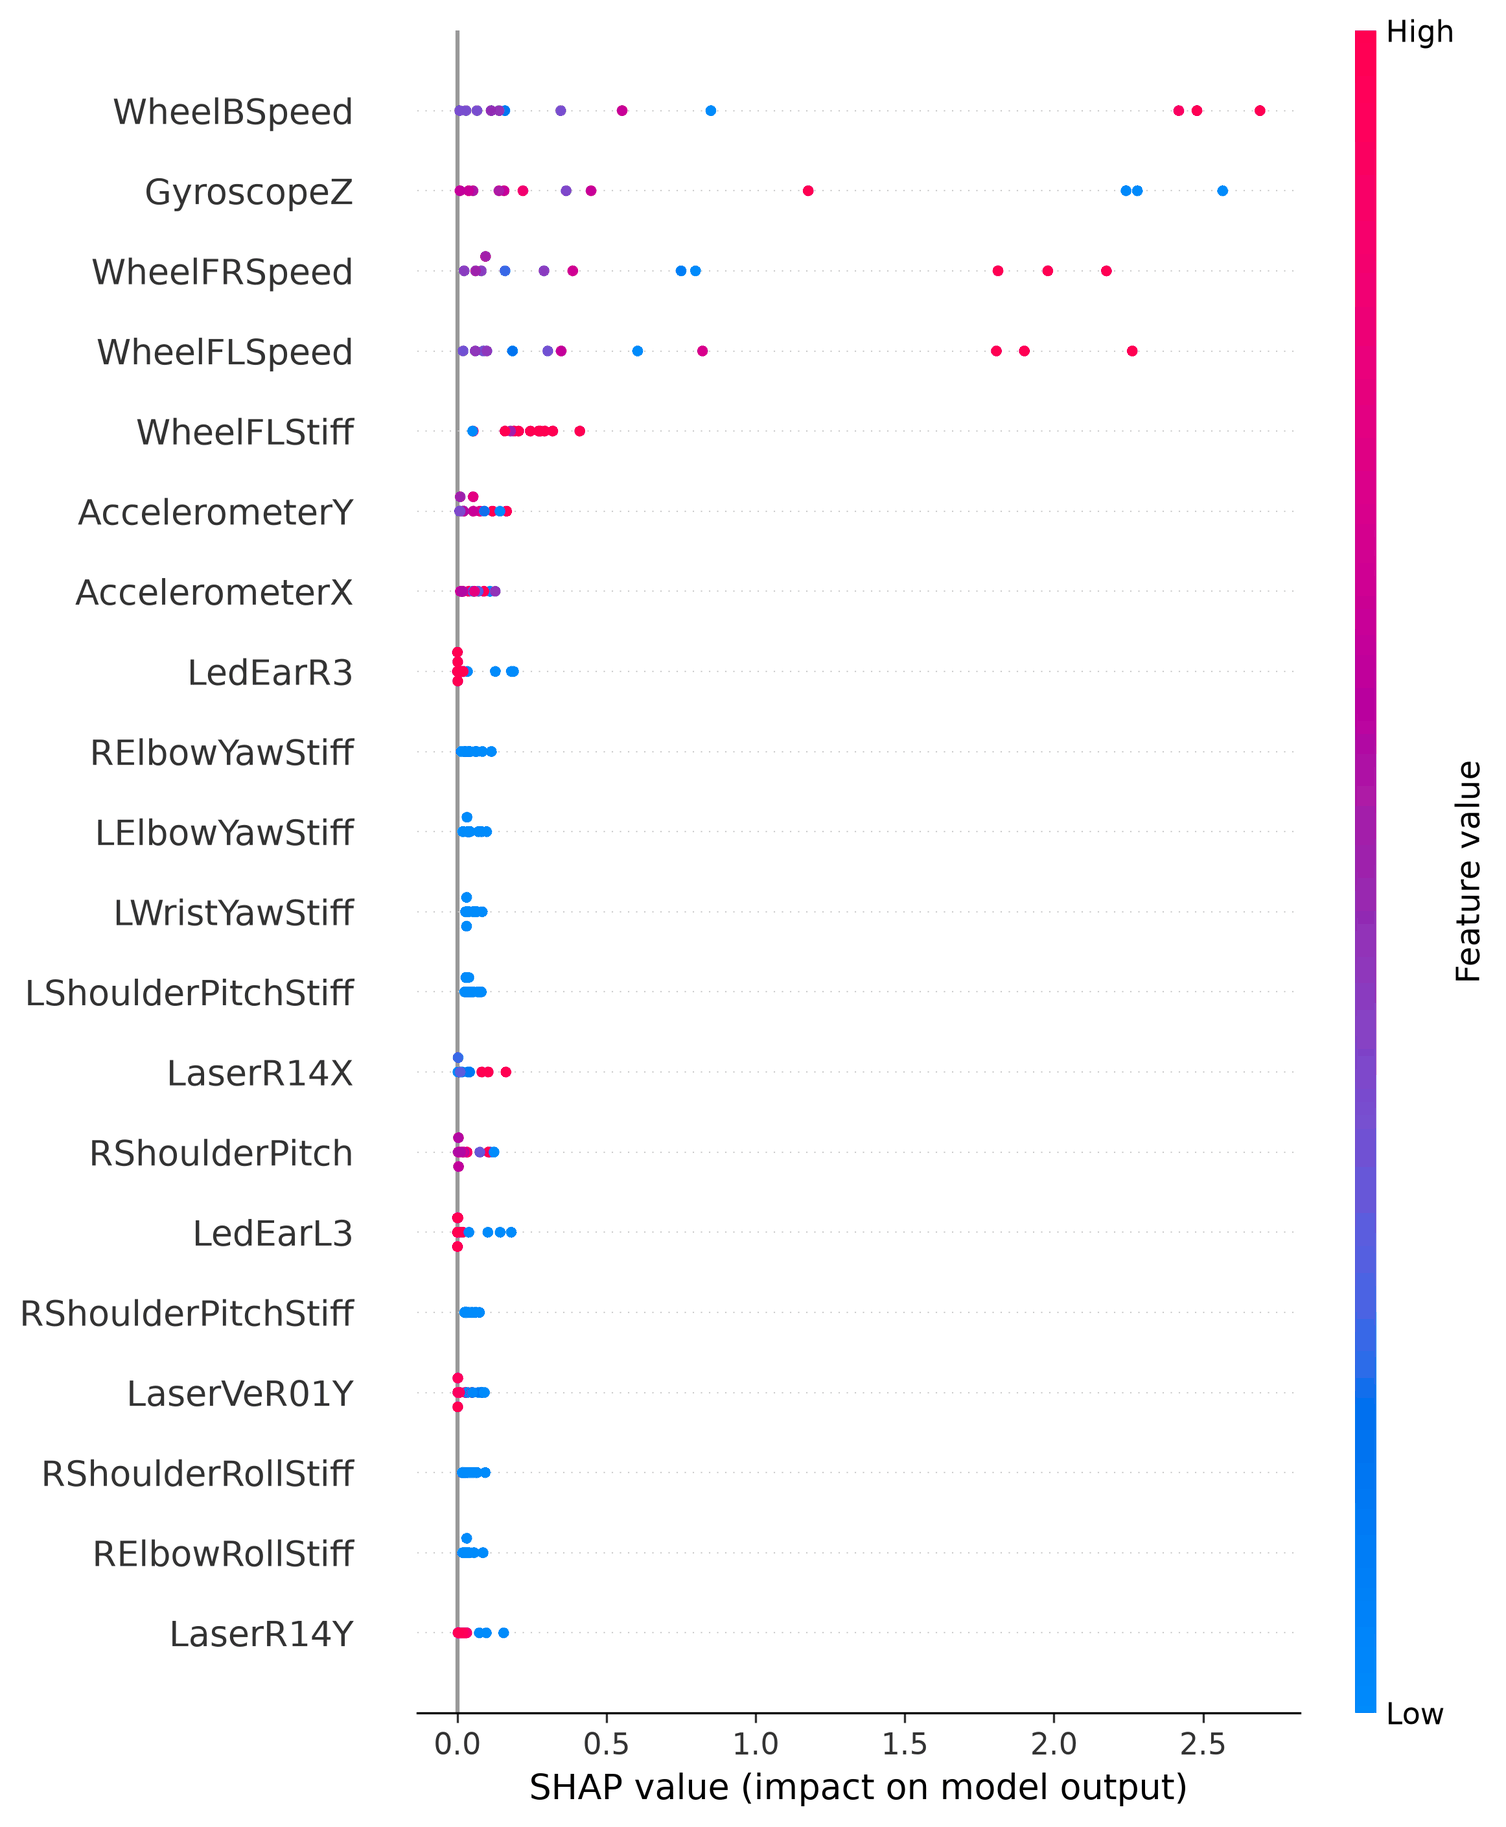
\includegraphics[width=0.85\textwidth,height=0.78\textheight,keepaspectratio]{baseline_shap_tcn_autoencoder_wheelscontrol.png}
  \caption[SHAP: TCN, WheelsControl]{SHAP attribution for the TCN autoencoder on the \texttt{WheelsControl} fault.}
  \label{fig:baseline-shap-tcn-autoencoder-wheelscontrol}
\end{figure}

\begin{figure}[htbp]
  \centering
  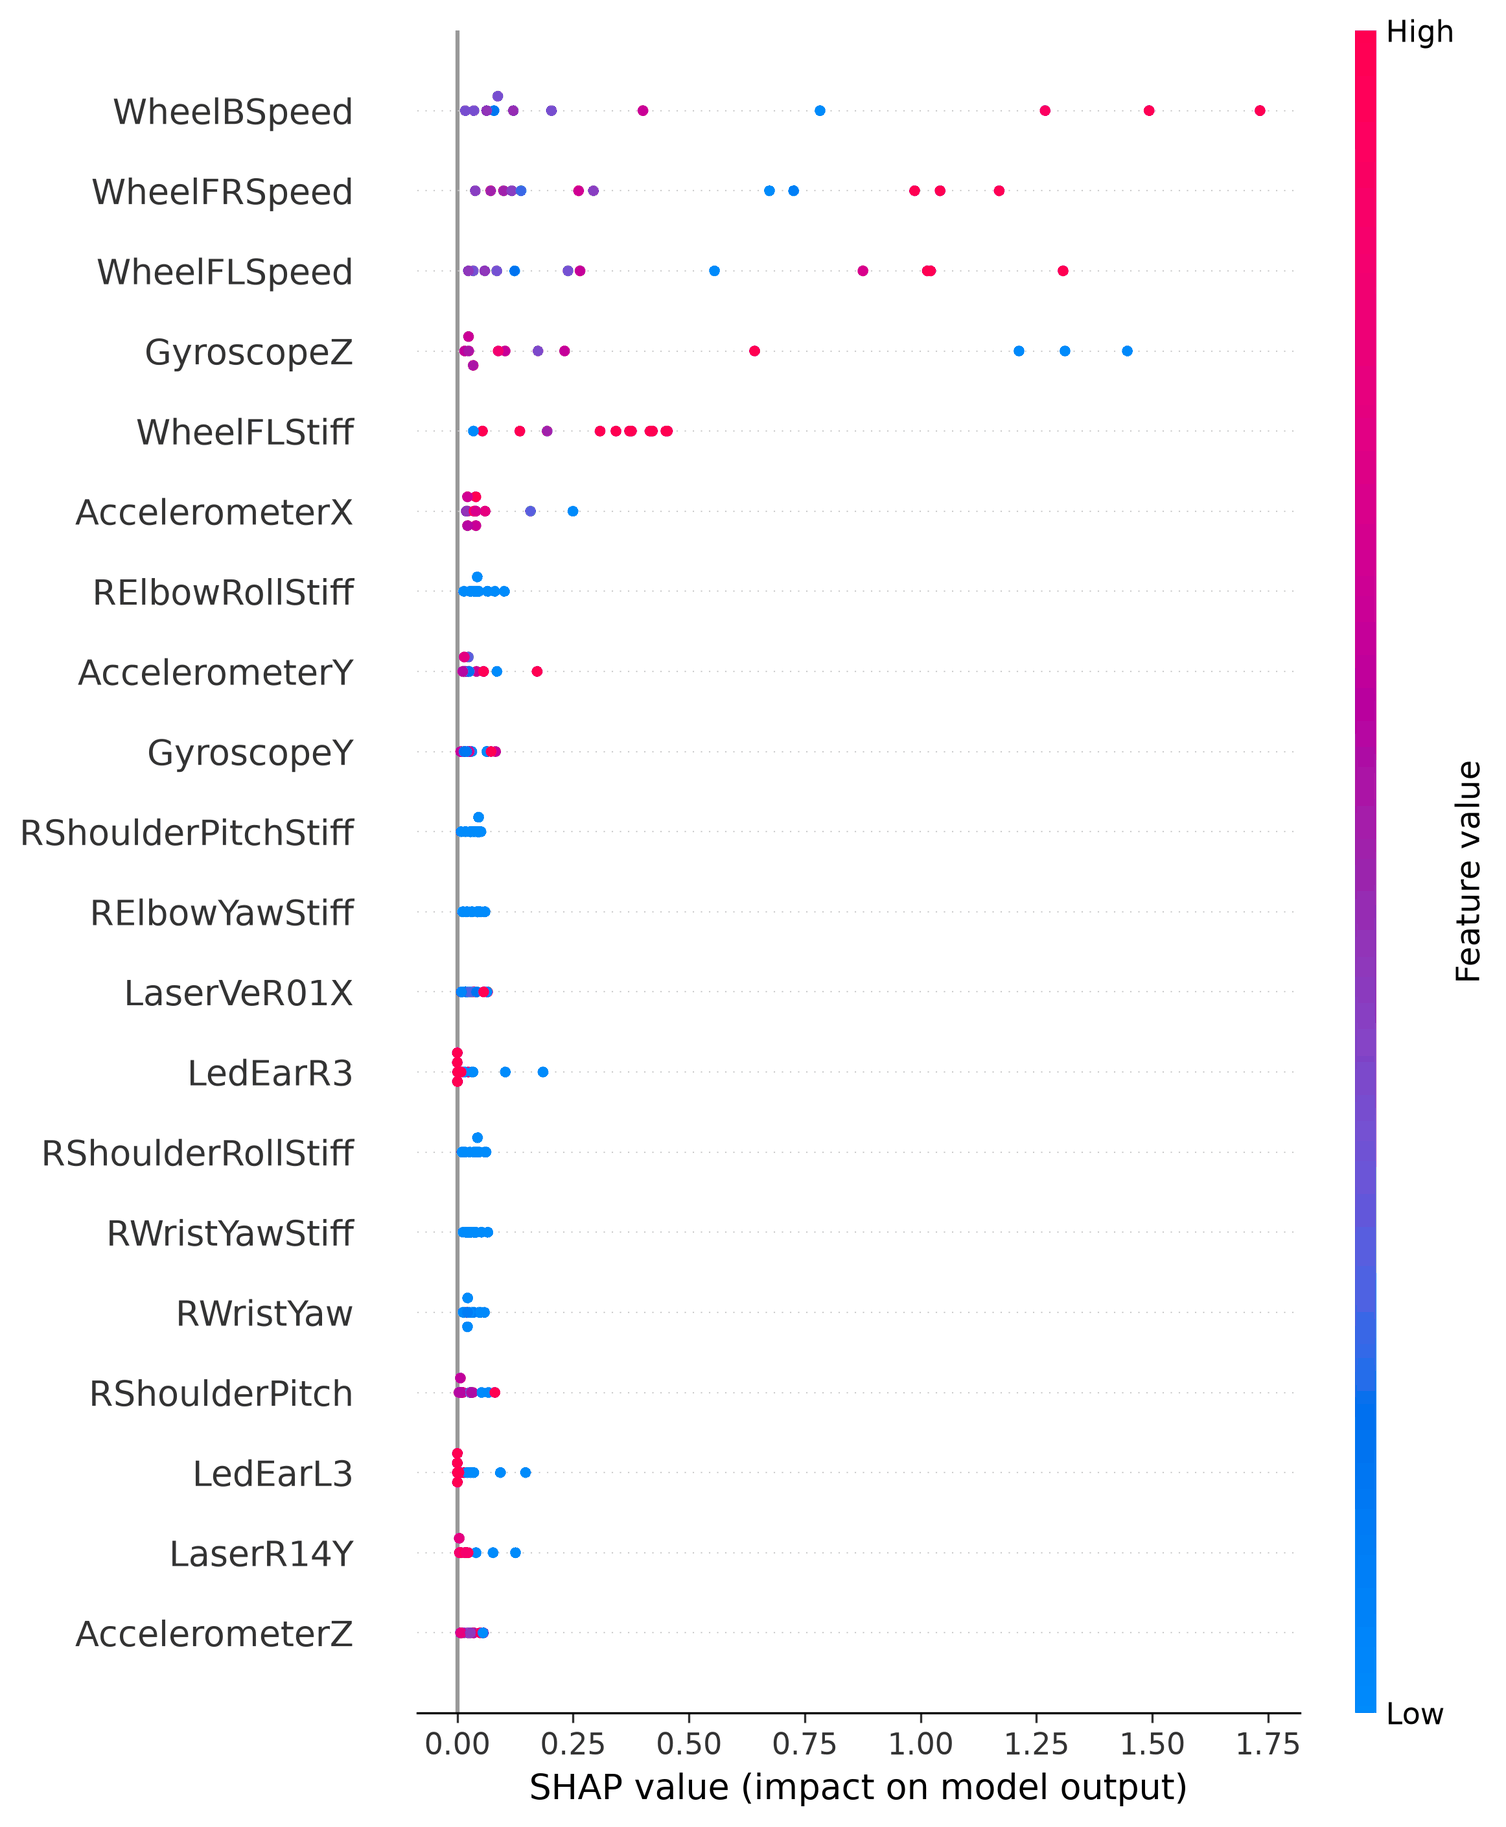
\includegraphics[width=0.85\textwidth,height=0.78\textheight,keepaspectratio]{baseline_shap_transformer_autoencoder_wheelscontrol.png}
  \caption[SHAP: Transformer, WheelsControl]{SHAP attribution for the Transformer autoencoder on the \texttt{WheelsControl} fault.}
  \label{fig:baseline-shap-transformer-autoencoder-wheelscontrol}
\end{figure}

The SHAP attributions for the other two domains are collected here. The explainer is run on all three datasets, as Section~\ref{sec:setup-shap} describes, and the relevance and consistency figures reported in Section~\ref{sec:attribution} are computed over every anomaly class in each. One class from each of the two non-robotics domains is plotted below as a representative panel, for each of the three architectures: Figures~\ref{fig:baseline-shap-lstm-attack1} to~\ref{fig:baseline-shap-transformer-fault1}. The electrocardiogram panels rank twelve leads and the plant panels rank fifty-two process variables, so the two are not on a common axis and are not meant to be read against one another; each is read against the causal attribution for the same domain. The same caution applies between the three architectures within one domain, for the reason Section~\ref{sec:shap-normalised} sets out: the explainer returns attributions in the units of the input, so the horizontal scale of a panel is fixed by what the model reads and not by how much of the record it explains. On the electrocardiogram class plotted here the largest attribution differs by more than two orders of magnitude between the widest panel and the narrowest. What is comparable across them is the ordering of the leads, not the width of the bars.

\begin{figure}[htbp]
  \centering
  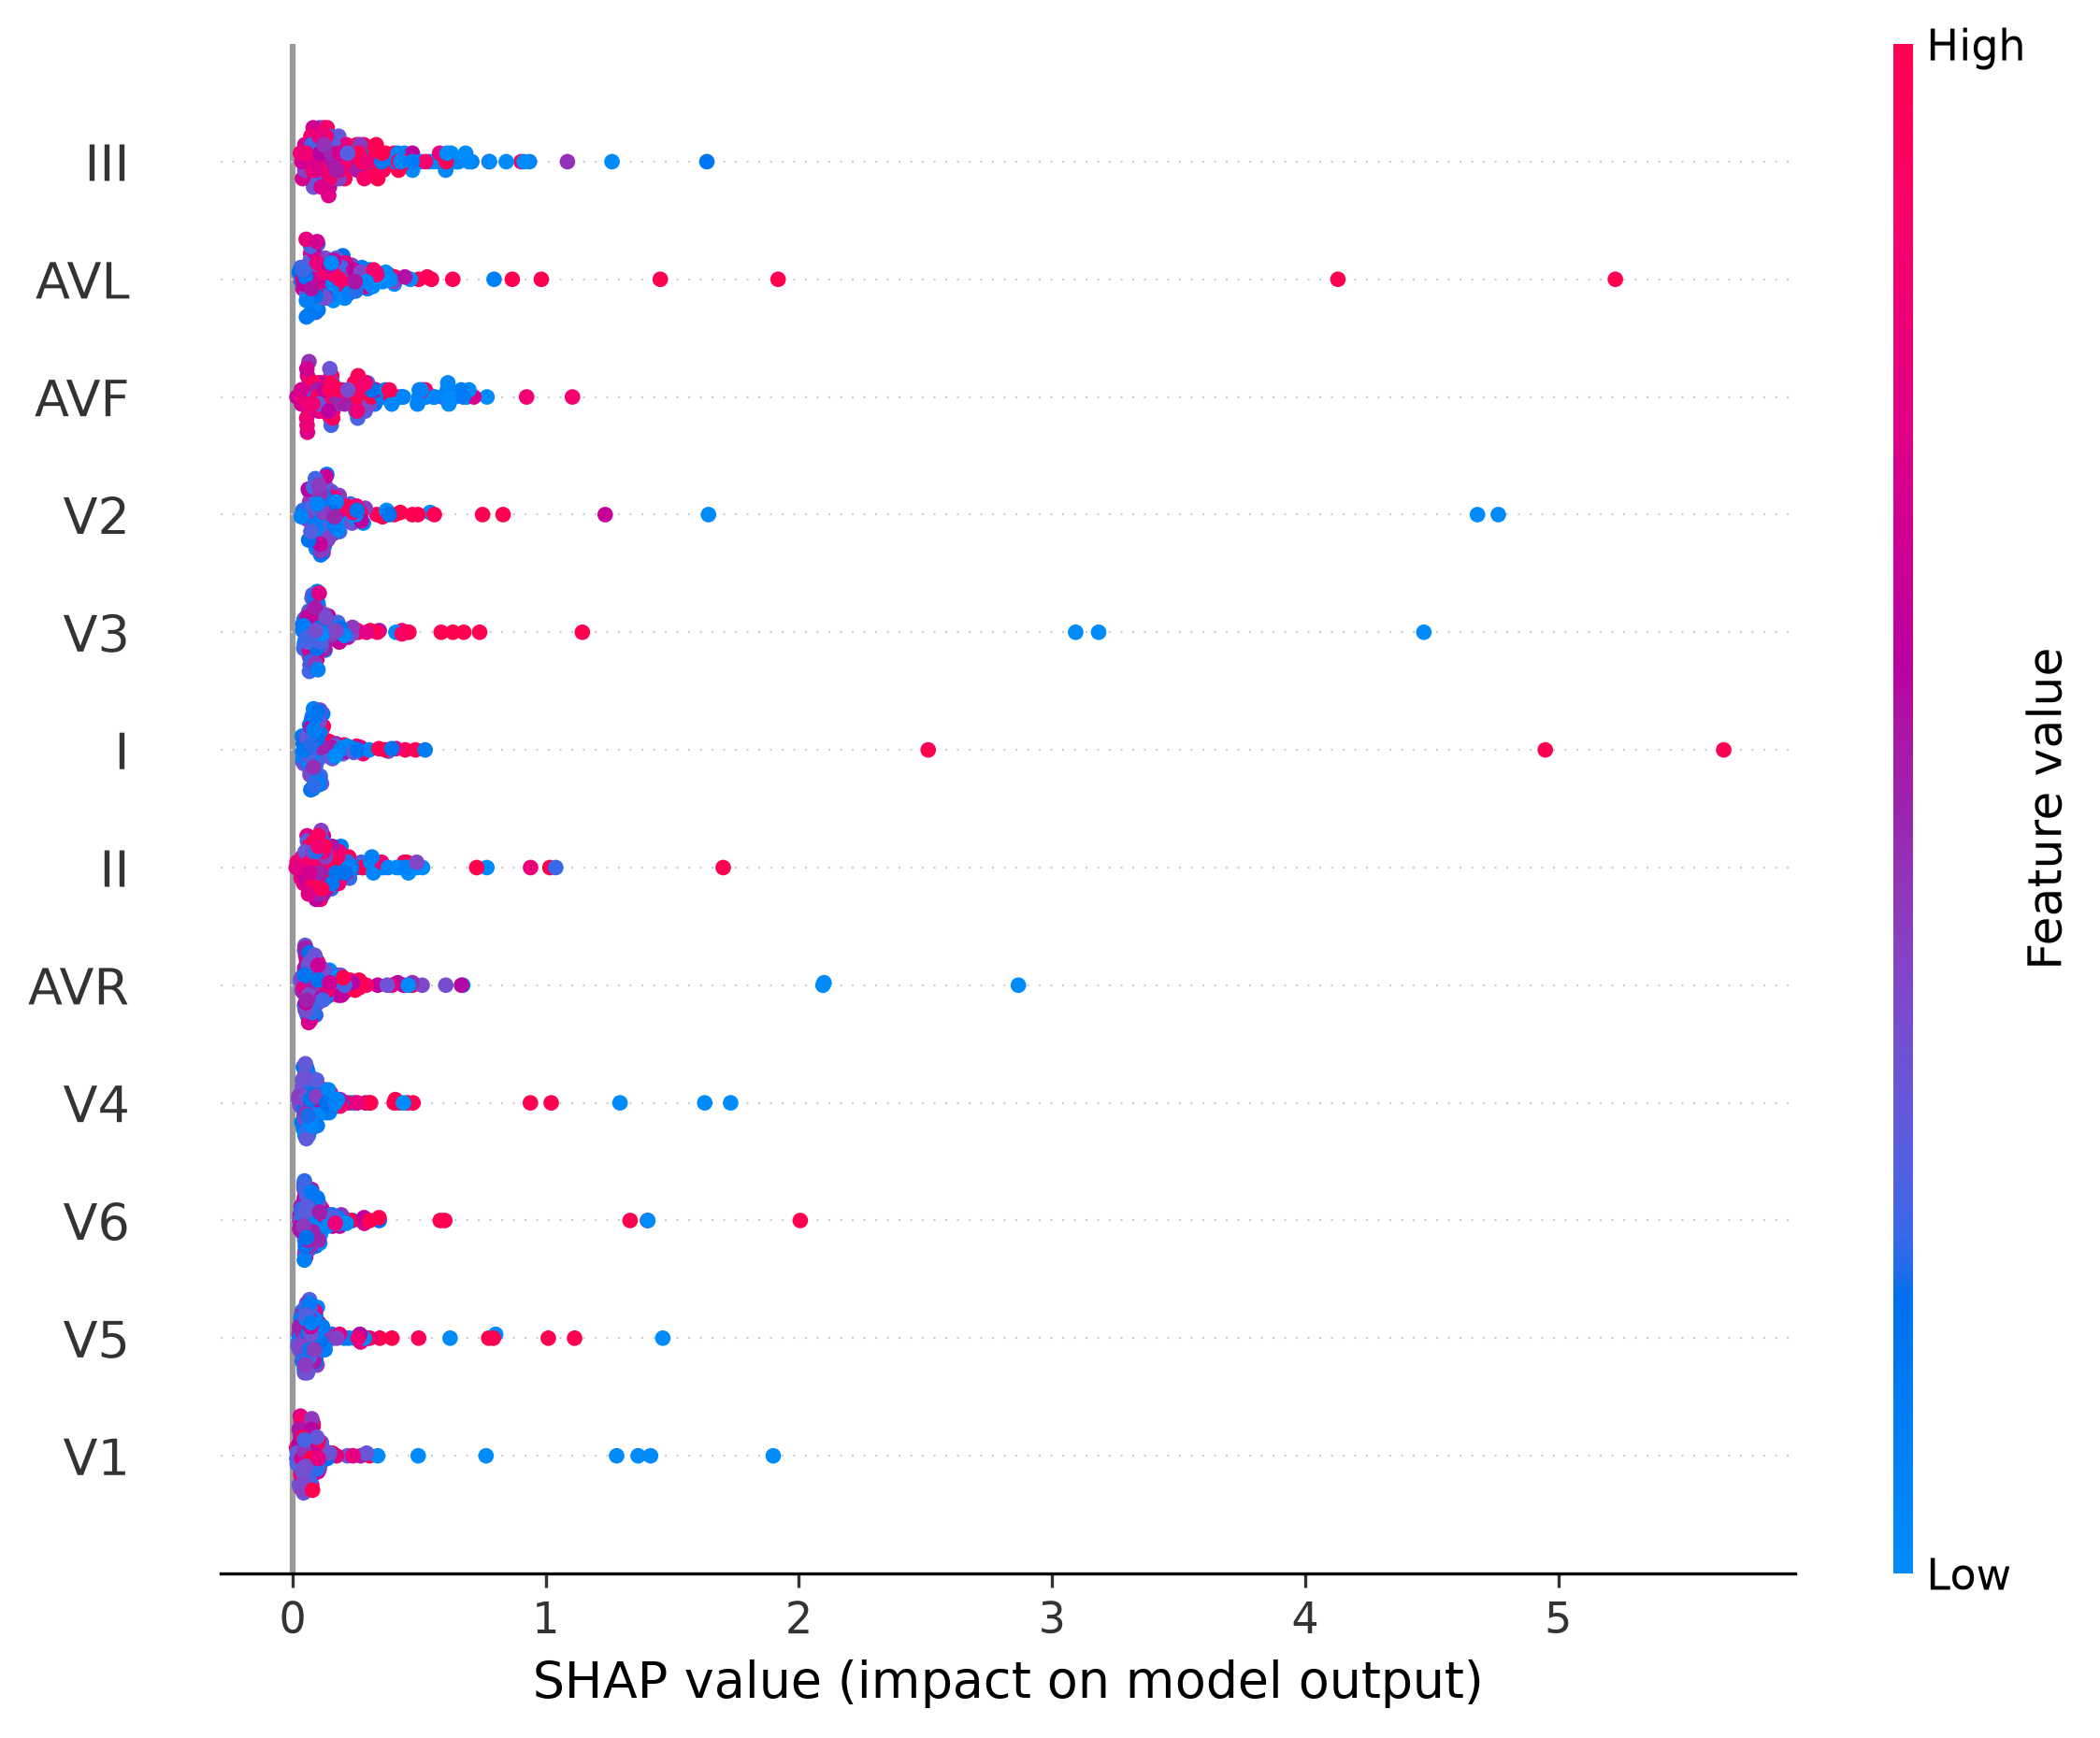
\includegraphics[width=0.85\textwidth,height=0.78\textheight,keepaspectratio]{baseline_shap_lstm_autoencoder_attack_1.png}
  \caption[SHAP: LSTM, PTB-XL]{SHAP attribution for the LSTM autoencoder on record class \texttt{Attack\_1} of the electrocardiogram domain.}
  \label{fig:baseline-shap-lstm-attack1}
\end{figure}

\begin{figure}[htbp]
  \centering
  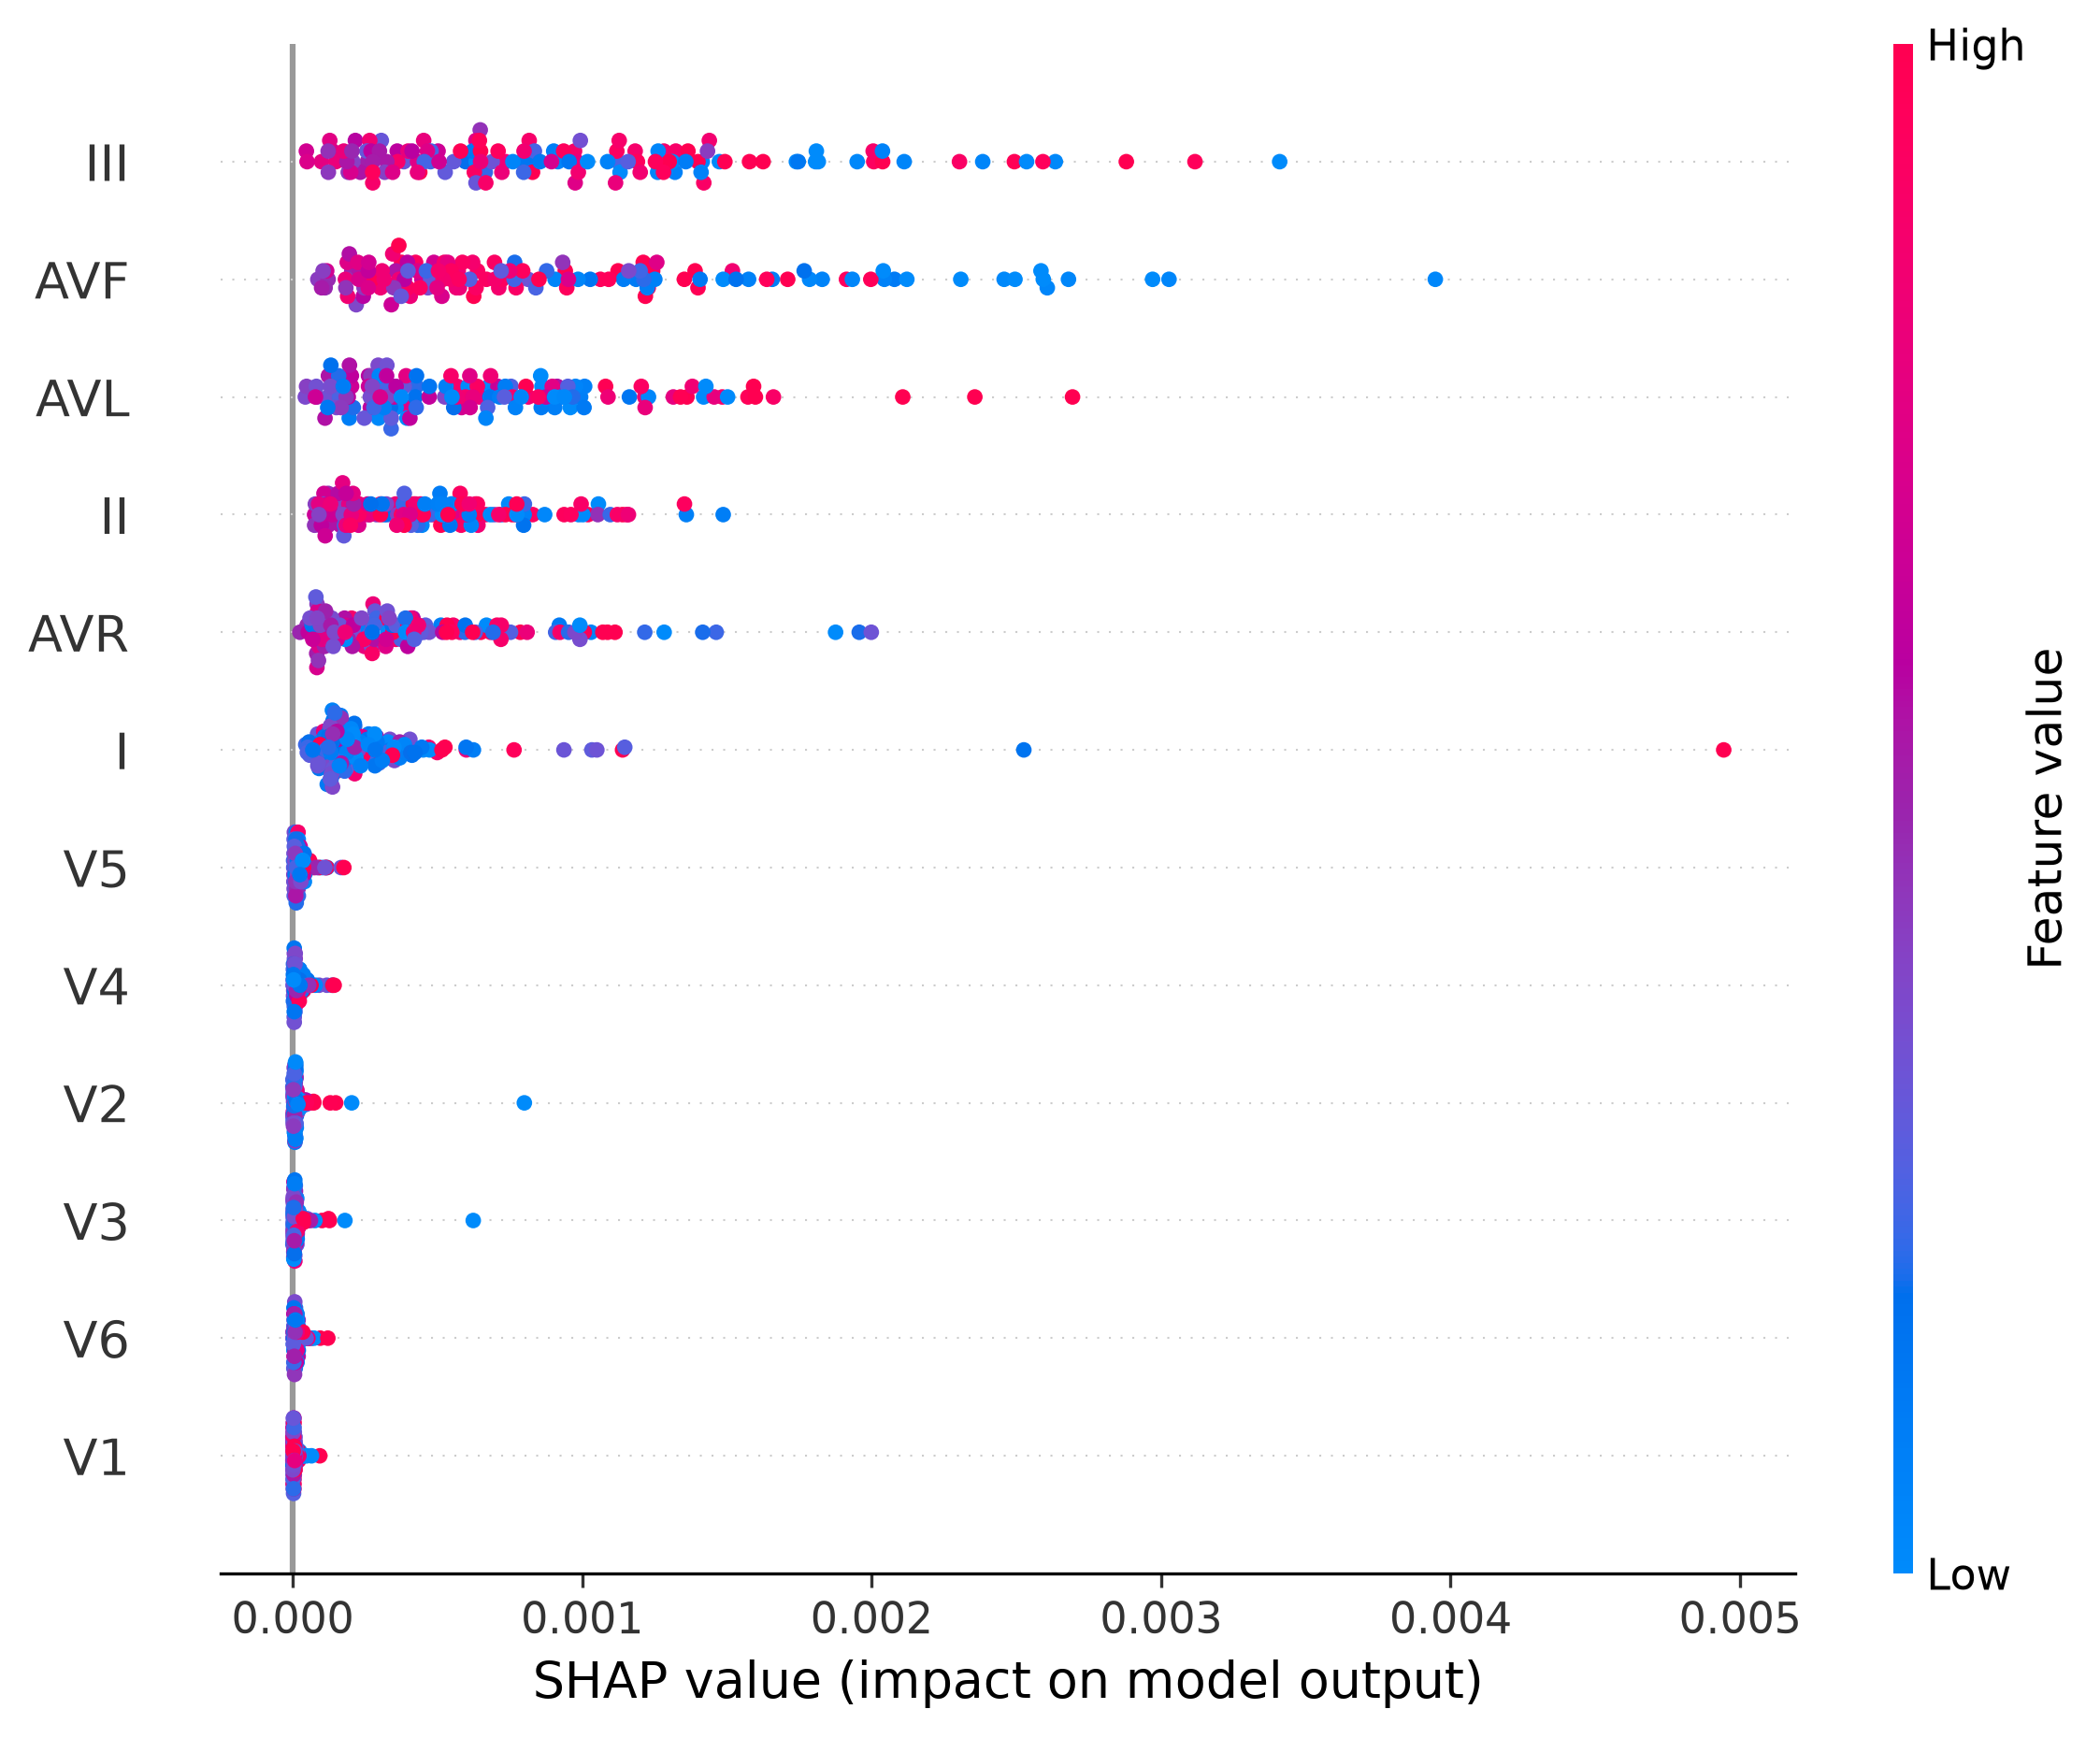
\includegraphics[width=0.85\textwidth,height=0.78\textheight,keepaspectratio]{baseline_shap_tcn_autoencoder_attack_1.png}
  \caption[SHAP: TCN, PTB-XL]{SHAP attribution for the TCN autoencoder on record class \texttt{Attack\_1} of the electrocardiogram domain.}
  \label{fig:baseline-shap-tcn-attack1}
\end{figure}

\begin{figure}[htbp]
  \centering
  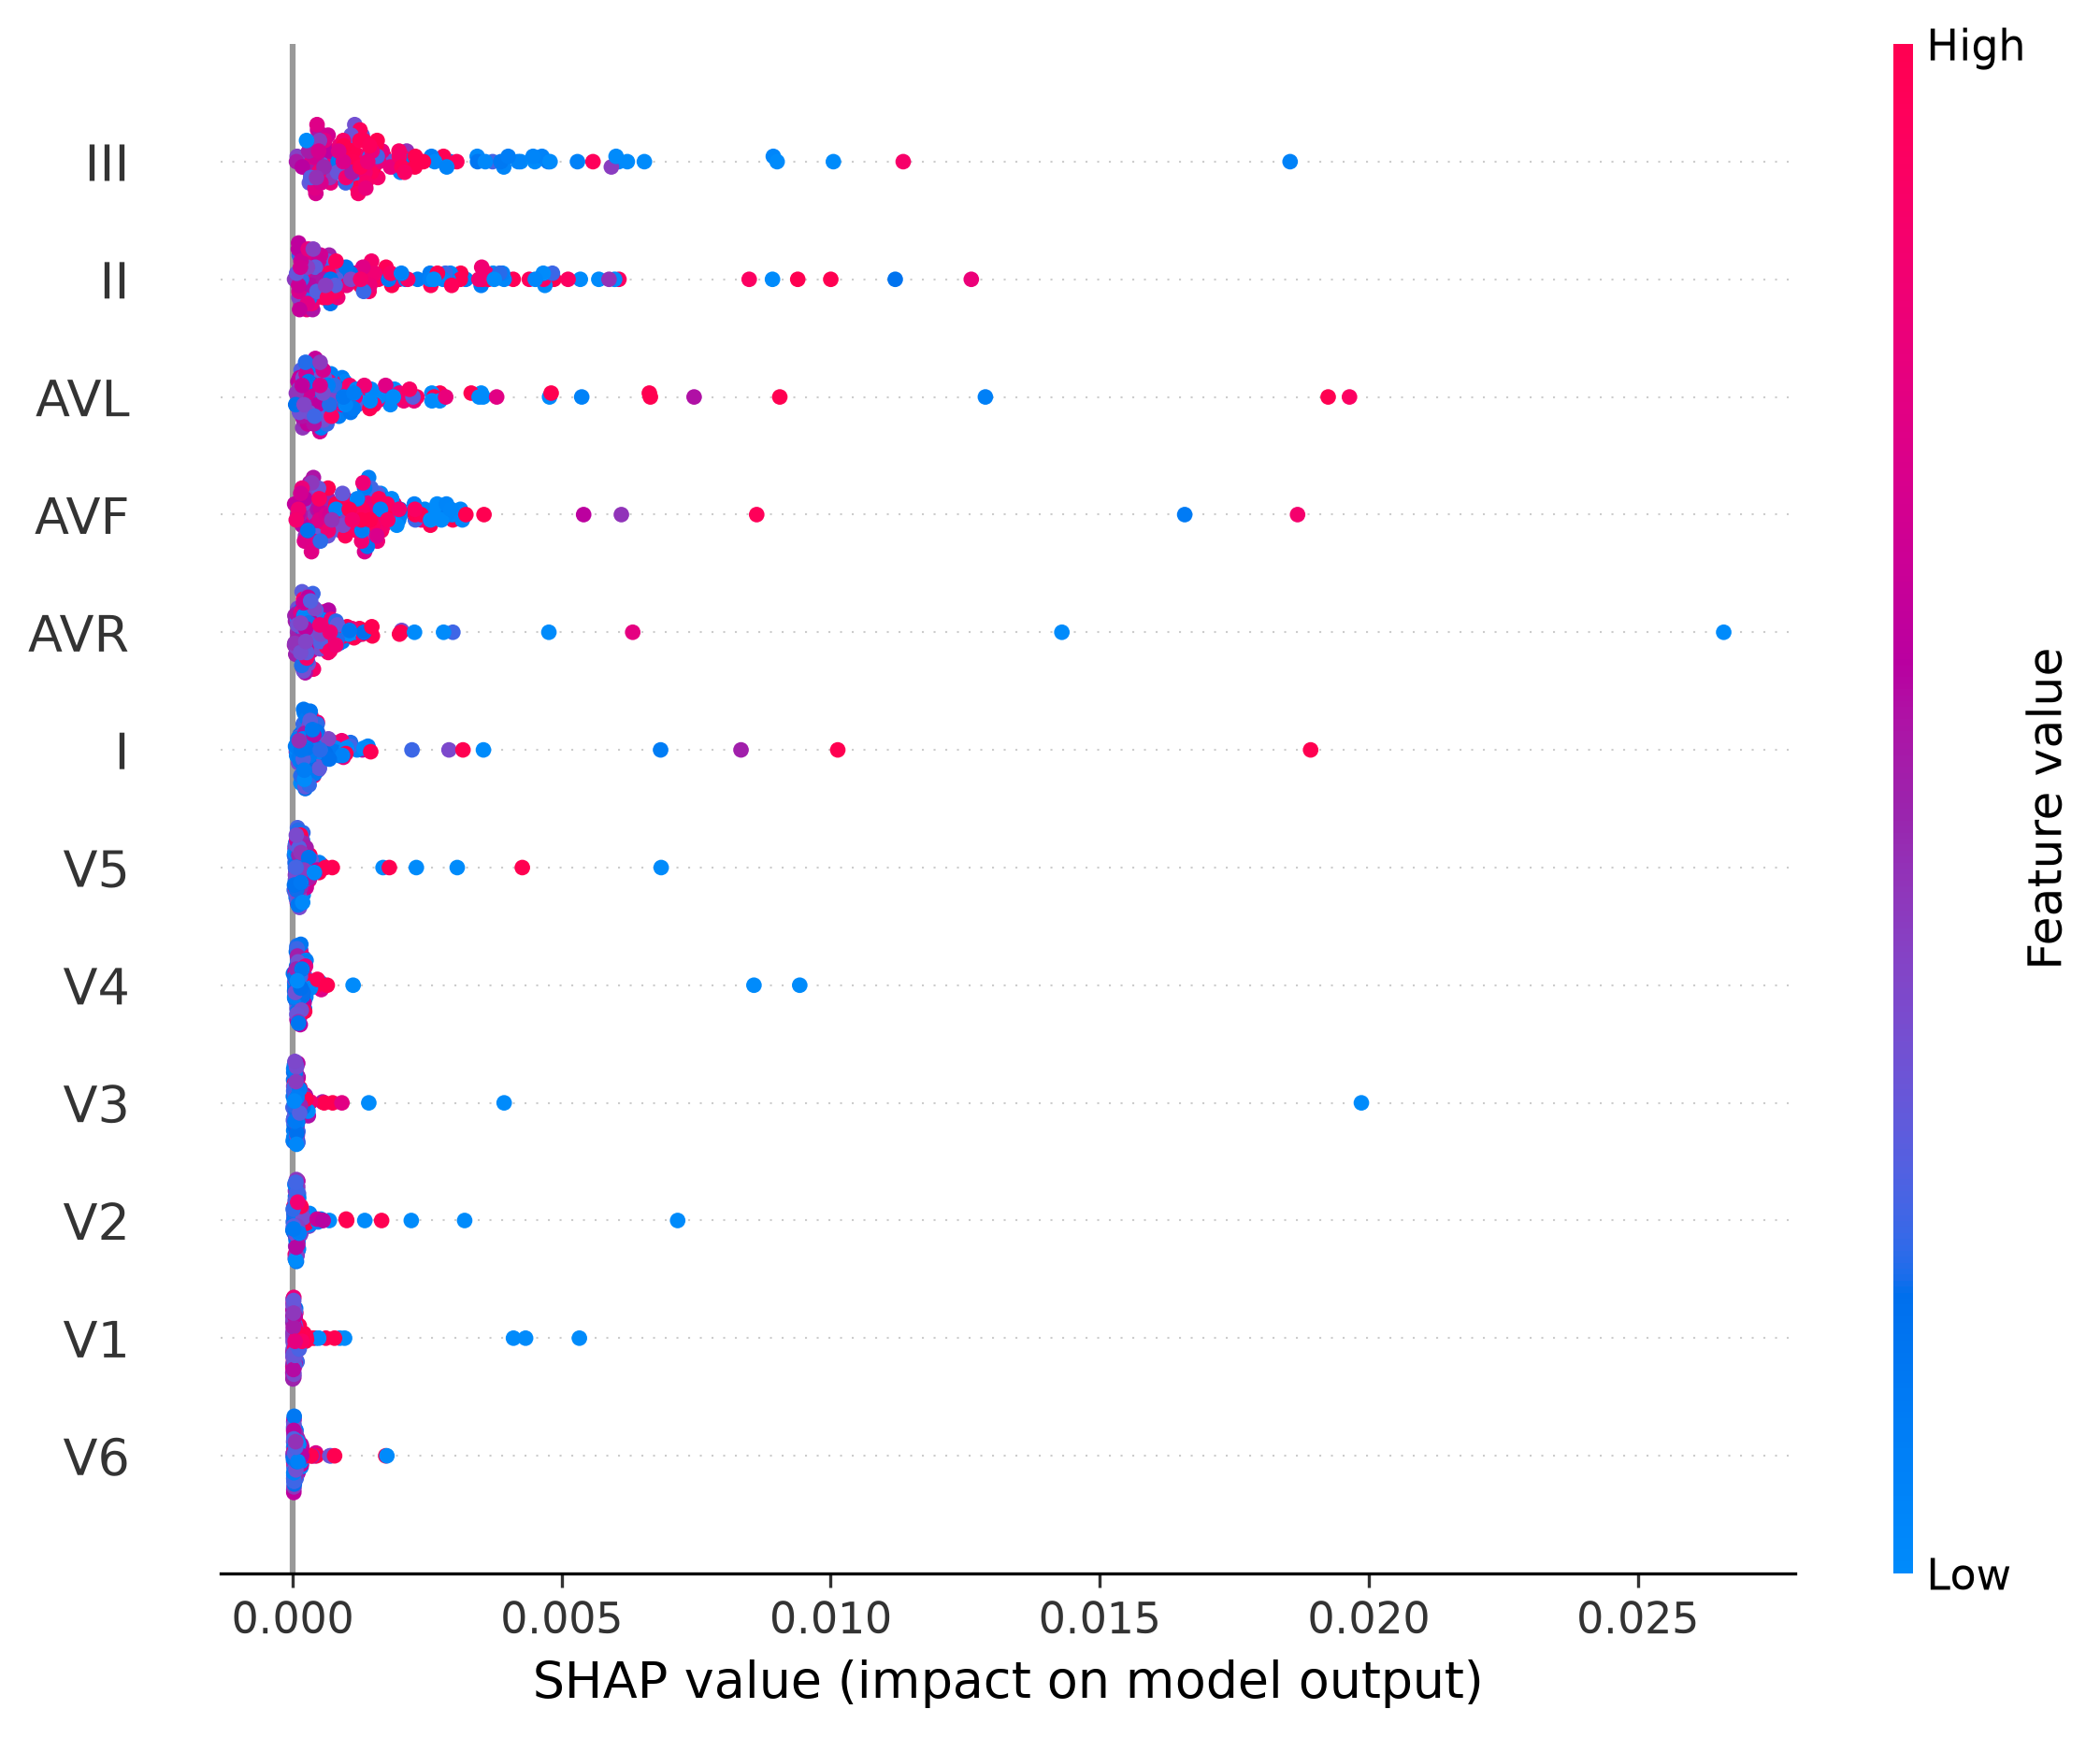
\includegraphics[width=0.85\textwidth,height=0.78\textheight,keepaspectratio]{baseline_shap_transformer_autoencoder_attack_1.png}
  \caption[SHAP: Transformer, PTB-XL]{SHAP attribution for the Transformer autoencoder on record class \texttt{Attack\_1} of the electrocardiogram domain.}
  \label{fig:baseline-shap-transformer-attack1}
\end{figure}

\begin{figure}[htbp]
  \centering
  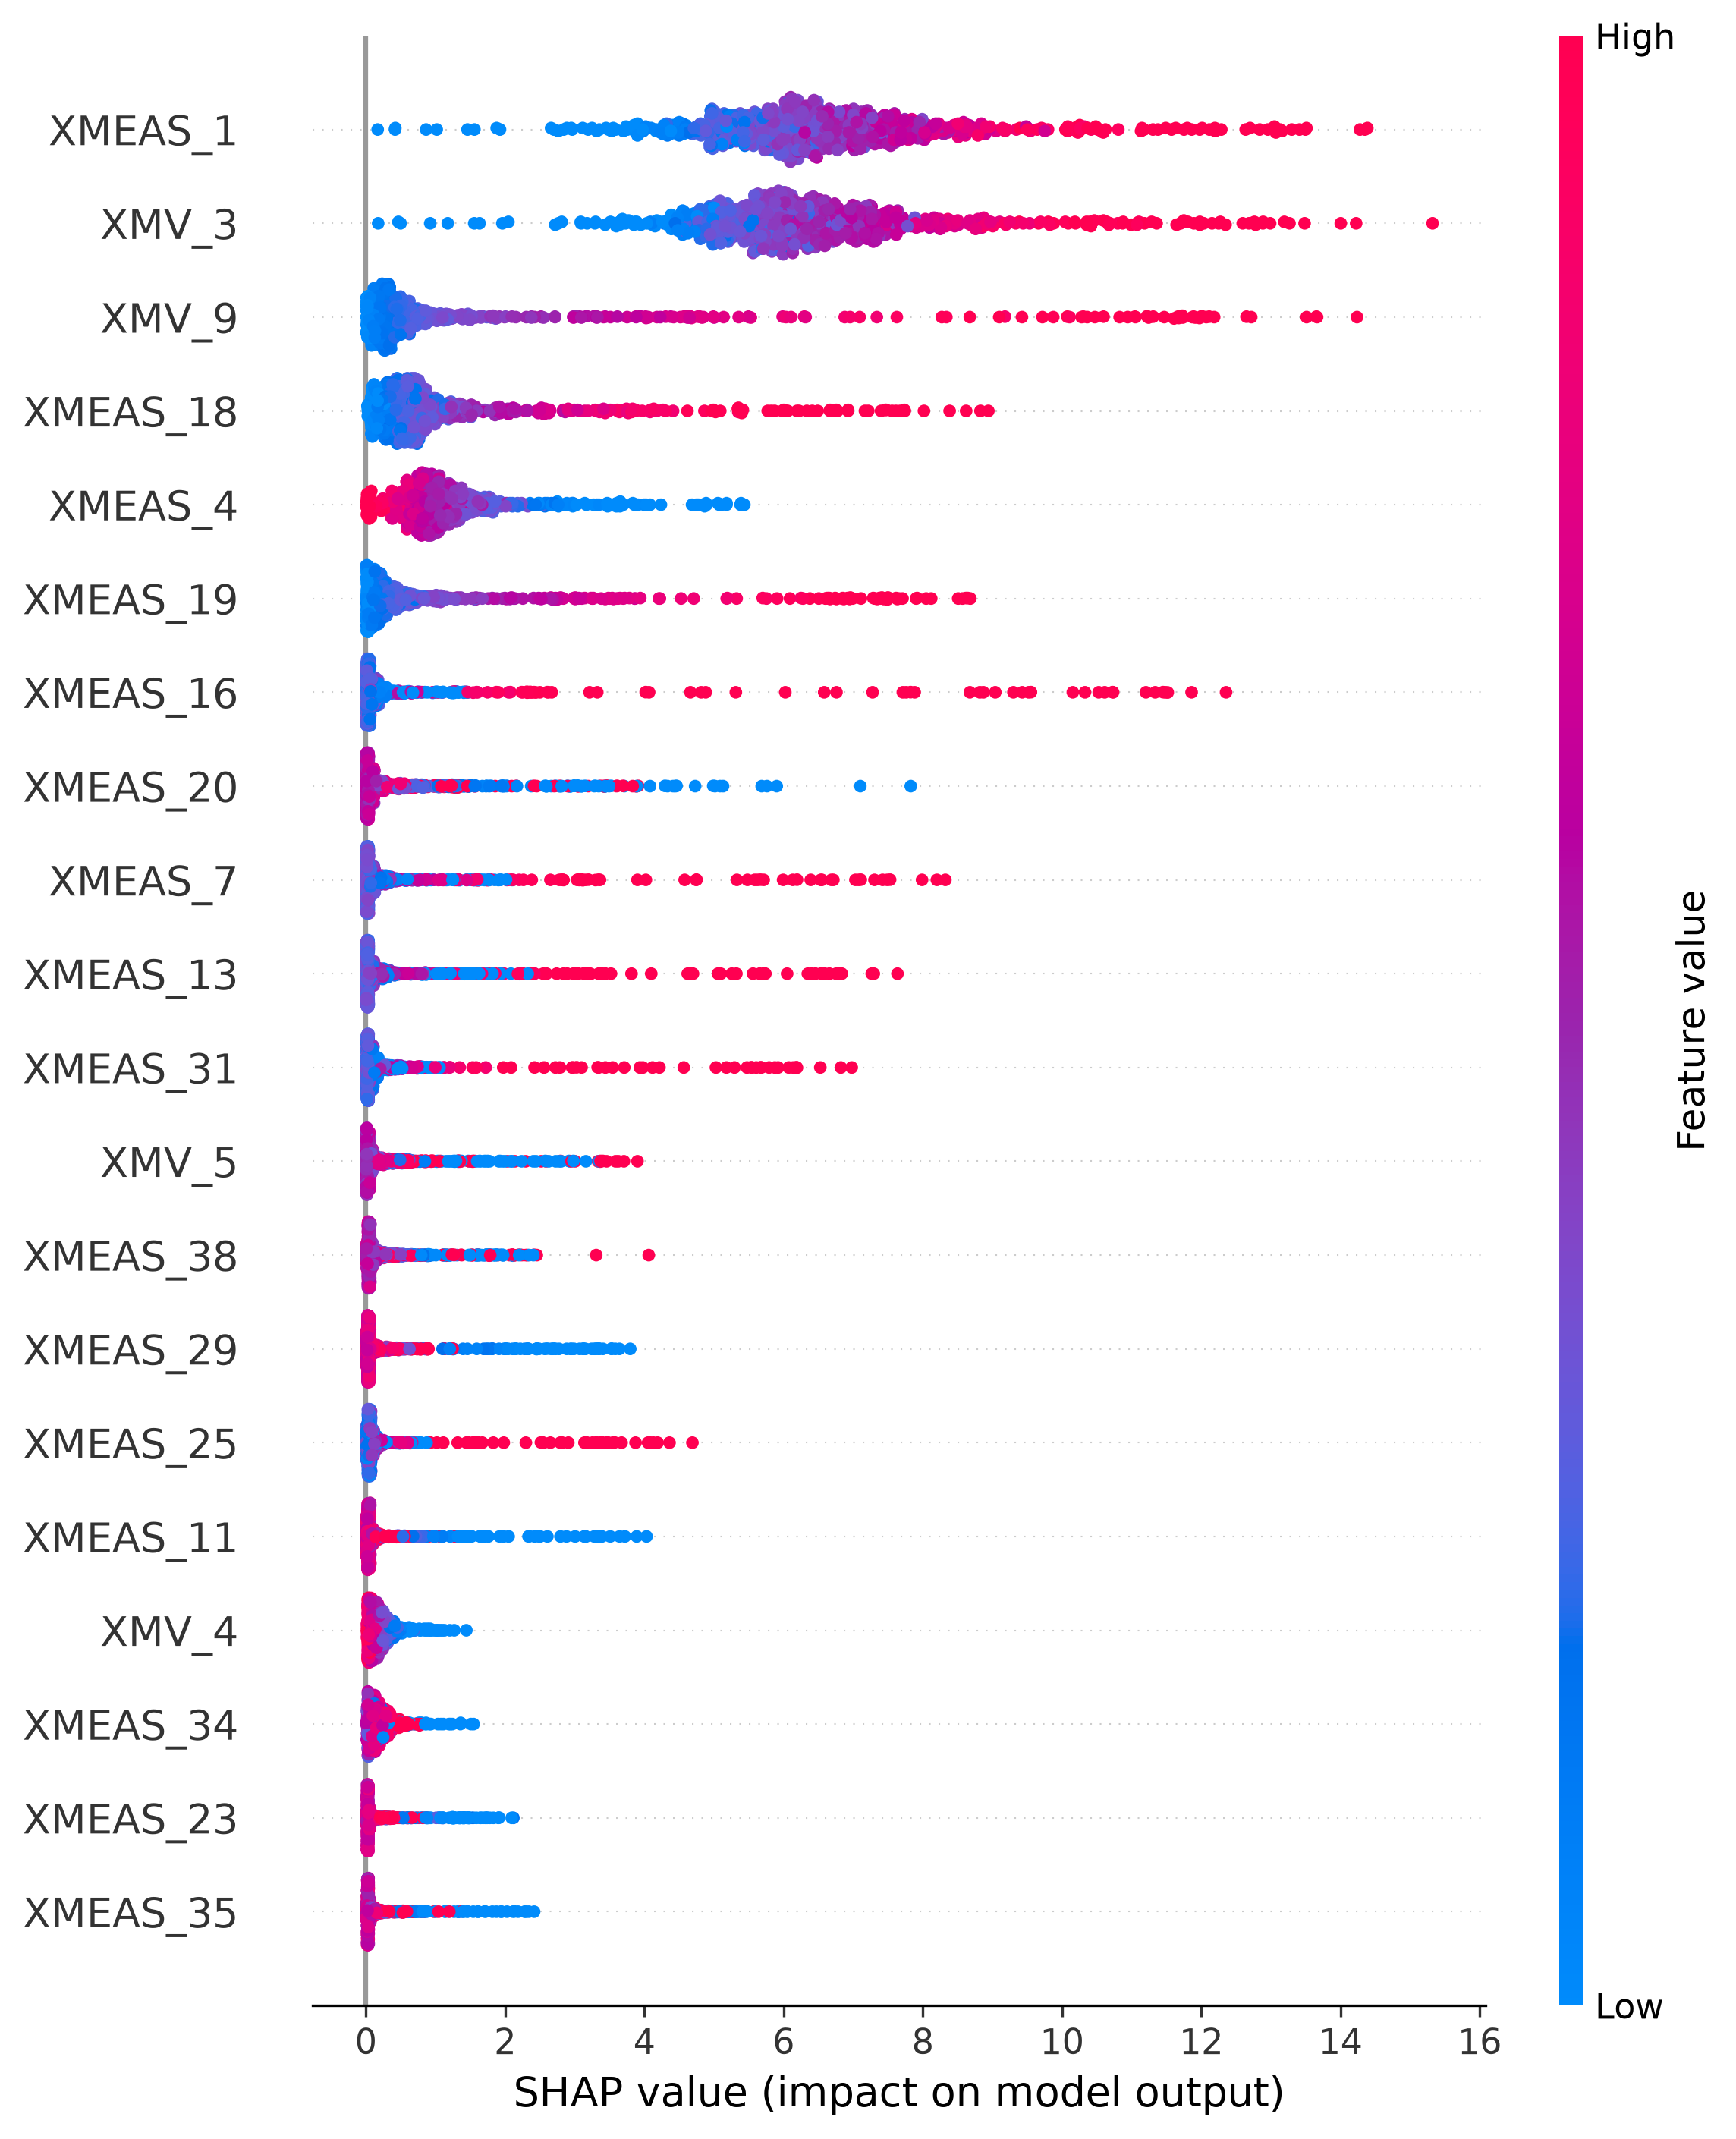
\includegraphics[width=0.85\textwidth,height=0.78\textheight,keepaspectratio]{baseline_shap_lstm_autoencoder_fault_1.png}
  \caption[SHAP: LSTM, TEP]{SHAP attribution for the LSTM autoencoder on \texttt{Fault\_1} of the Tennessee Eastman domain.}
  \label{fig:baseline-shap-lstm-fault1}
\end{figure}

\begin{figure}[htbp]
  \centering
  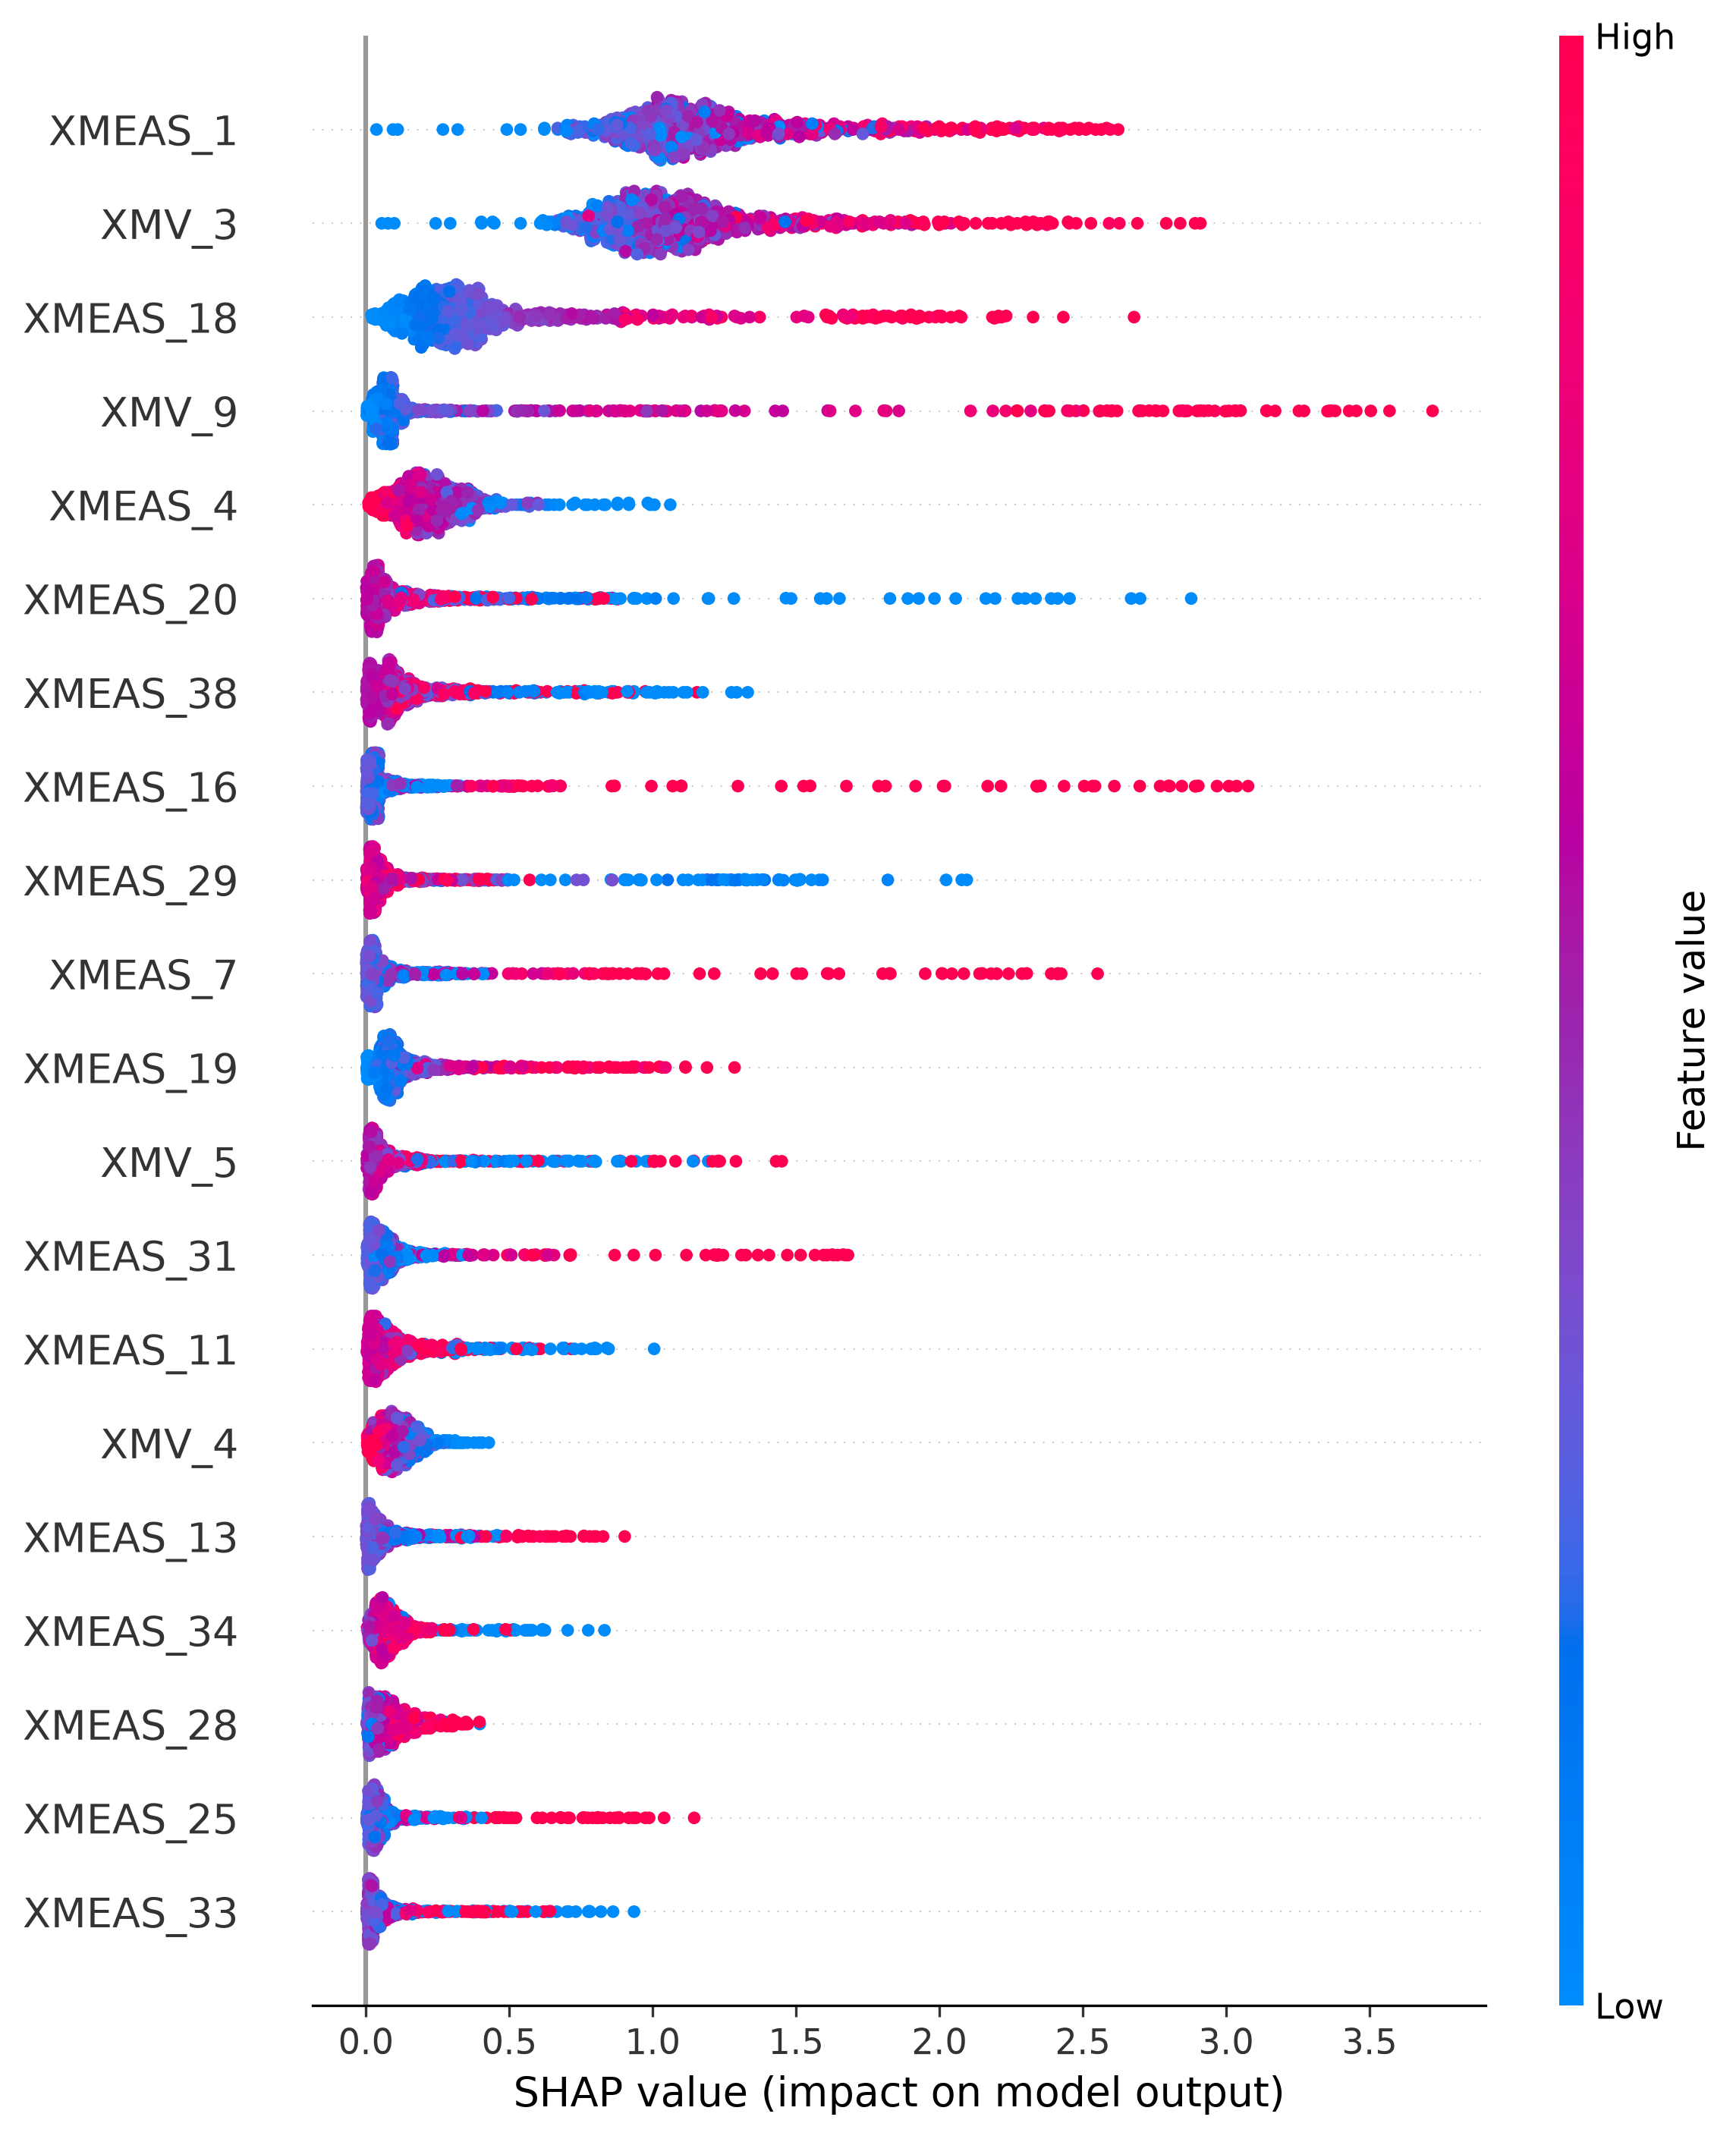
\includegraphics[width=0.85\textwidth,height=0.78\textheight,keepaspectratio]{baseline_shap_tcn_autoencoder_fault_1.png}
  \caption[SHAP: TCN, TEP]{SHAP attribution for the TCN autoencoder on \texttt{Fault\_1} of the Tennessee Eastman domain.}
  \label{fig:baseline-shap-tcn-fault1}
\end{figure}

\begin{figure}[htbp]
  \centering
  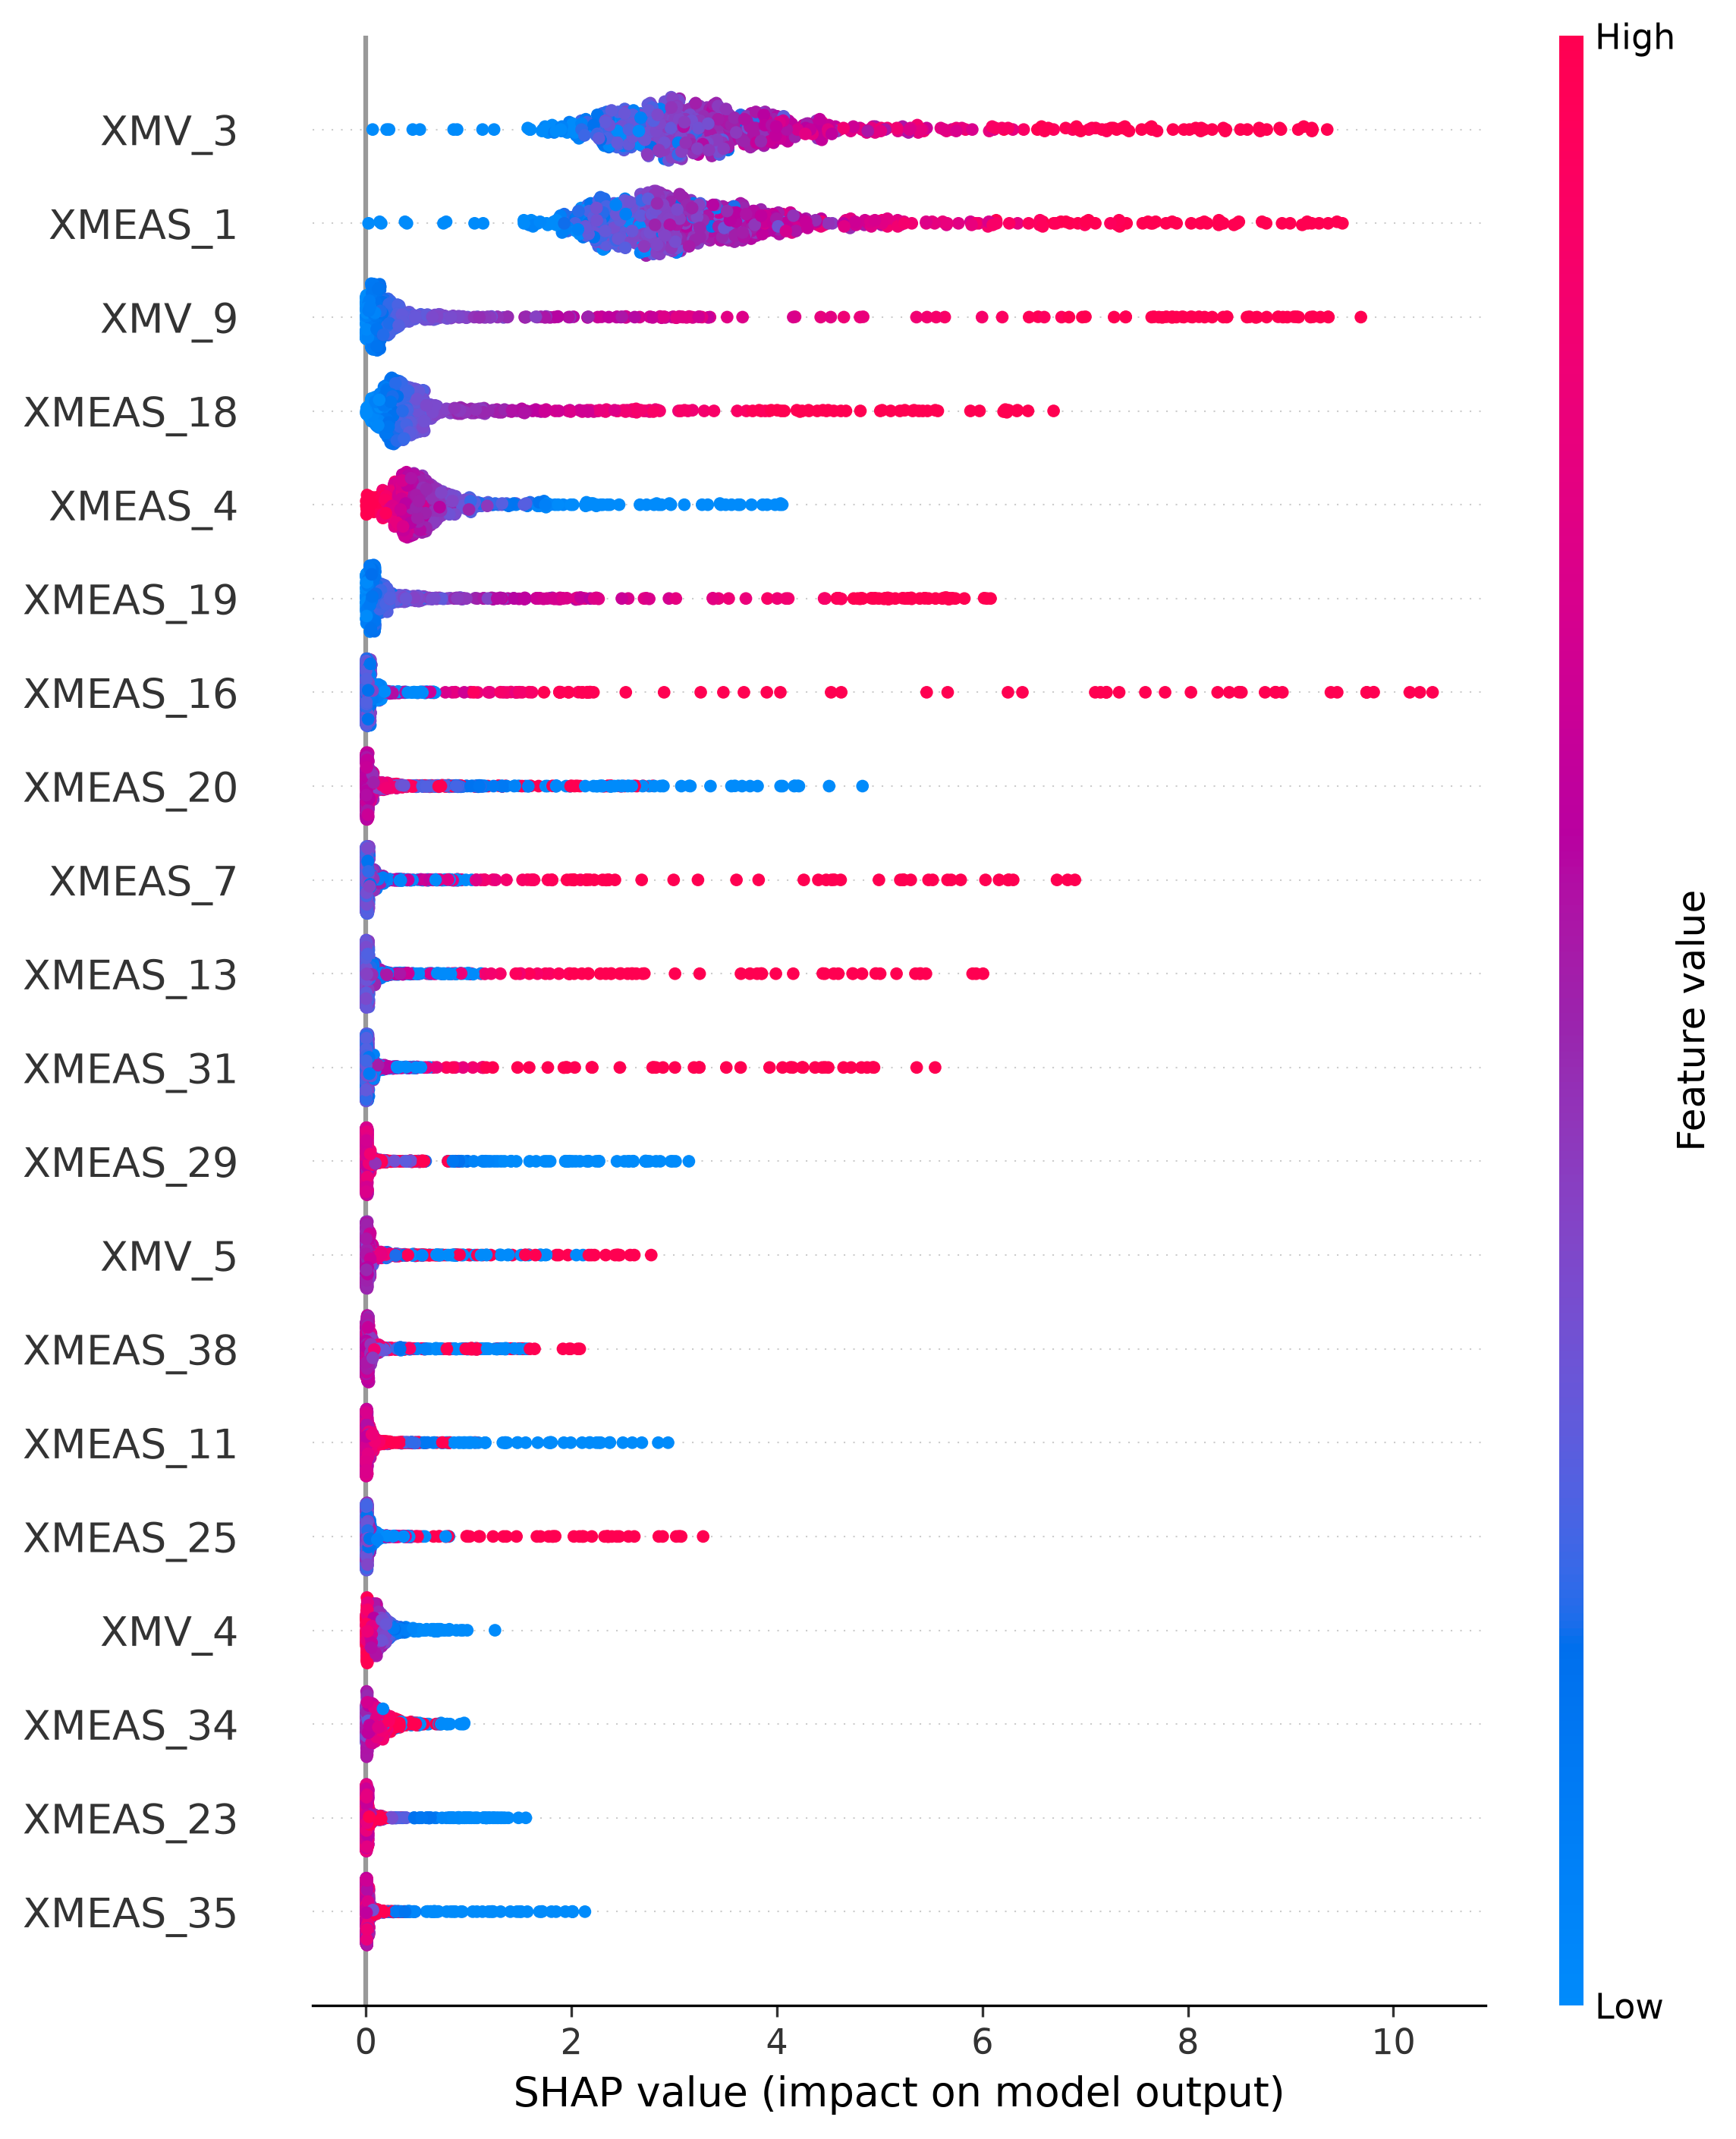
\includegraphics[width=0.85\textwidth,height=0.78\textheight,keepaspectratio]{baseline_shap_transformer_autoencoder_fault_1.png}
  \caption[SHAP: Transformer, TEP]{SHAP attribution for the Transformer autoencoder on \texttt{Fault\_1} of the Tennessee Eastman domain.}
  \label{fig:baseline-shap-transformer-fault1}
\end{figure}

\begin{figure}[htbp]
  \centering
  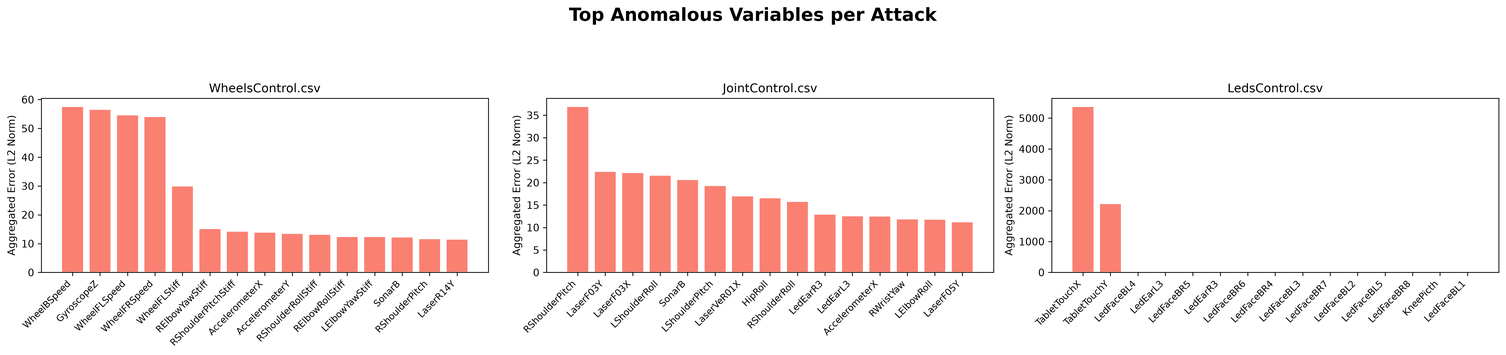
\includegraphics[width=0.85\textwidth,height=0.78\textheight,keepaspectratio]{baseline_lstm_autoencoder_top_anomalous_variables.png}
  \caption[Reconstruction ranking: LSTM baseline]{Top anomalous variables per attack class for the LSTM autoencoder baseline, ranked by reconstruction error rather than by coefficient drift.}
  \label{fig:baseline-lstm-top}
\end{figure}


Figure~\ref{fig:baseline-lstm-top} gives the neural baseline's own ranking of anomalous variables, by reconstruction error rather than by coefficient drift.

\subsection{Normalising the SHAP Attributions}
\label{sec:shap-normalised}

The SHAP magnitudes plotted in Figures~\ref{fig:shap-lstm-leds}
to~\ref{fig:shap-transformer-leds} are small in absolute terms, and that
appearance is an artefact of the axis. GradientExplainer returns attributions in
the units of the input, so the magnitude of a panel is fixed by whatever scale
the sensors happen to be recorded in. Across the nine robot panels the largest
attribution ranges from 0.22 to 227.26, which is three orders of magnitude of
sensor scaling and not three orders of magnitude of explanation.

Normalising each panel by its own total attribution removes the scale and leaves
the share of the explanation that a variable carries, which is comparable across
architectures and faults. Figure~\ref{fig:shap-normalised} shows the LED fault on
that scale. The reference line is the 0.41\% a variable would receive if
the model spread attribution evenly over all 244 sensors. The top variable
carries between 2.3 and 68.2\% depending on the architecture, so the
attributions concentrate between 6 and 166 times more than an even spread. The
TCN is the extreme case, placing 95.9\% of its attribution on the top
three variables, while the LSTM places 6.3\% there and spreads the rest
almost flat. Read on the normalised scale the SHAP values are not small, and the
architectures differ from each other far more than the raw plots suggest.

\begin{figure}[htbp]
  \centering
  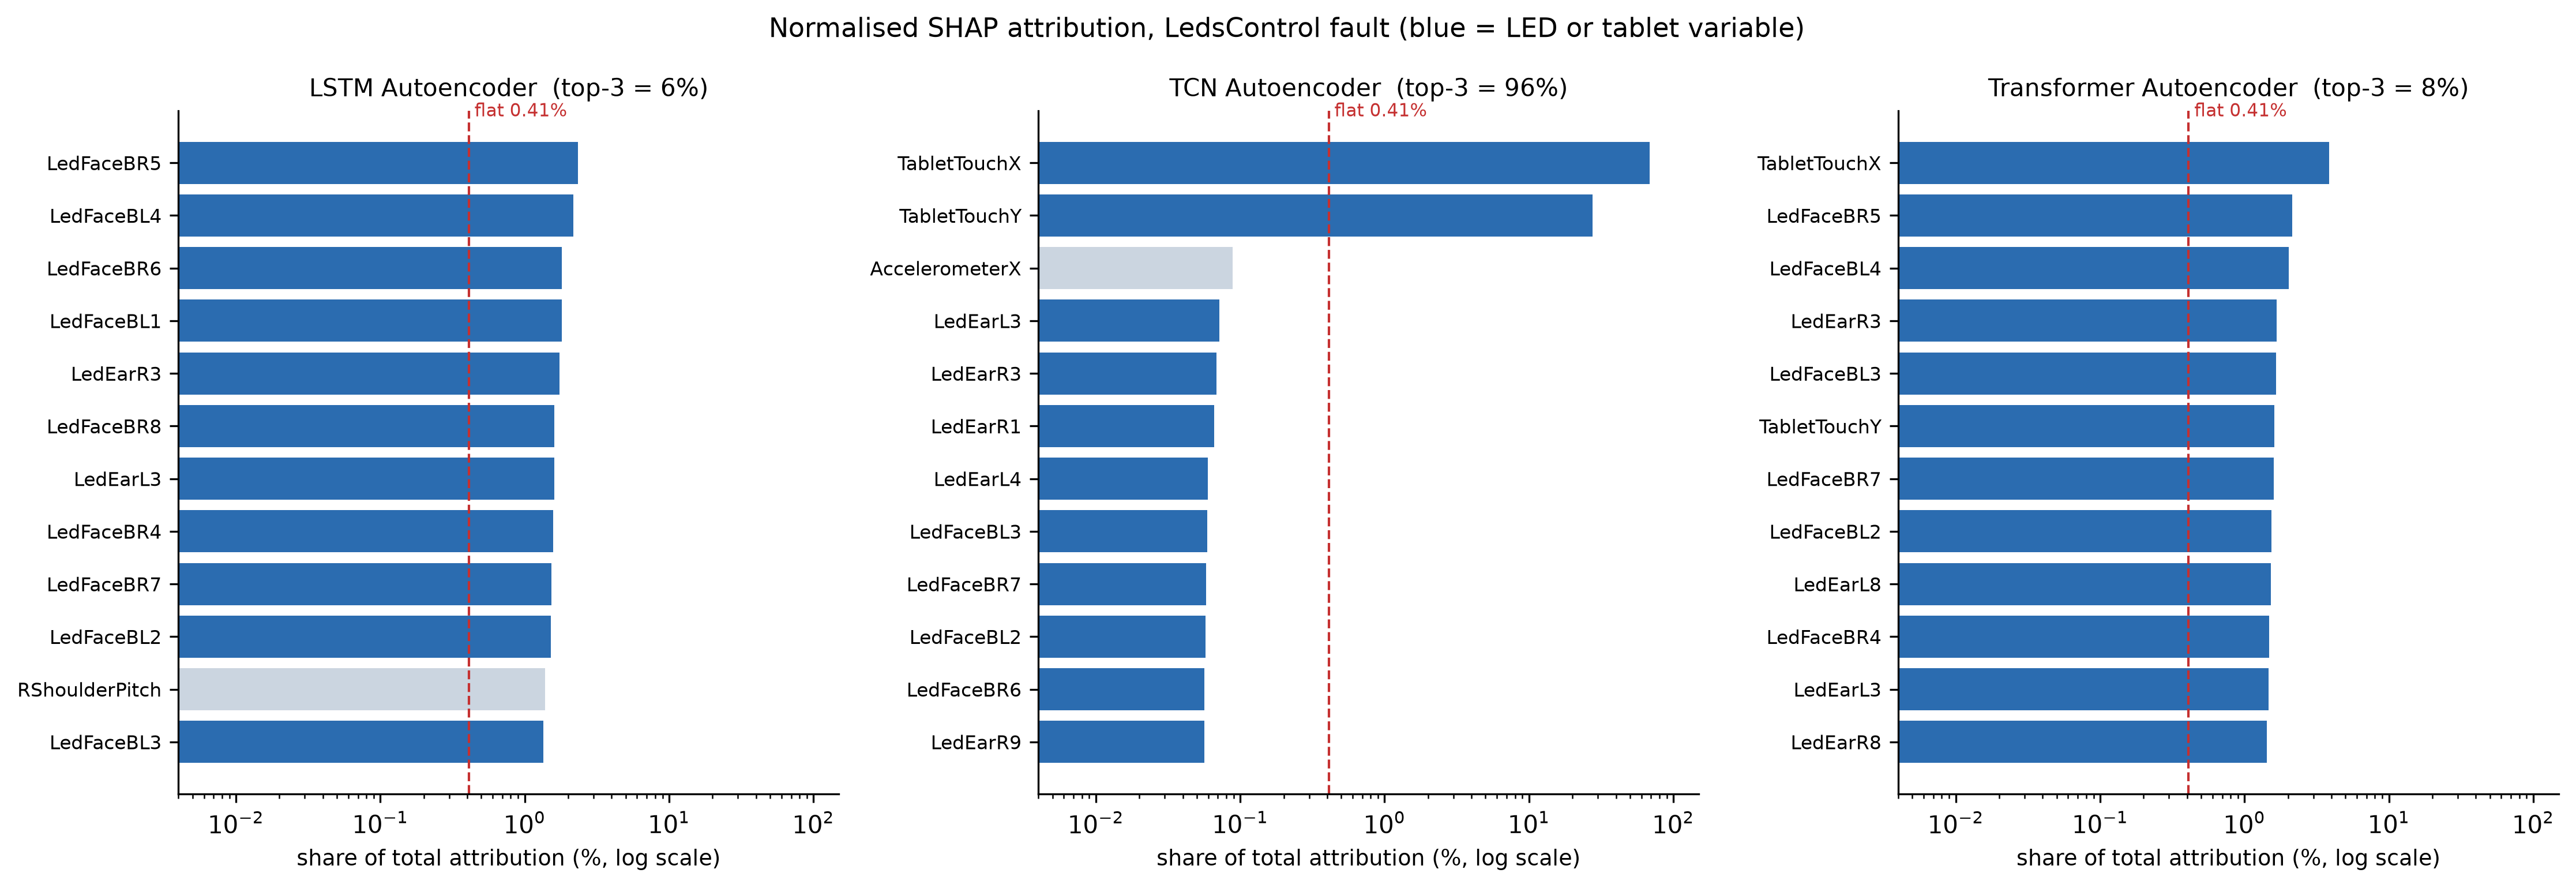
\includegraphics[width=\textwidth]{baseline_shap_normalised_ledscontrol.png}
  \caption[Normalised SHAP attribution for the \texttt{LedsControl} fault across the three neural architectures, on a common logarithmic scale]{Normalised SHAP attribution for the \texttt{LedsControl} fault across
  the three neural architectures, on a common logarithmic scale. Each bar is the
  share of that panel's total attribution. Blue marks a LED or tablet variable.
  The dashed line is the 0.41\% an evenly spreading model would assign.}
  \label{fig:shap-normalised}
\end{figure}

\section{Every Paired Attribution Comparison}
\label{app:attr-paired-full}

Chapter~\ref{ch:results} reports the paired attribution comparison at the top-three depth, which Section~\ref{sec:method-attribution} fixes as the depth every attribution result in this thesis is stated at. The other three depths are exploratory, and they are given here in full rather than summarised, because the alternative is to choose which of four depths to show after seeing what each one says.

One of them reverses the ordering. That reversal is why this table exists. At ten variables on the electrocardiogram GES leads SHAP by 9.0 points with thirteen of the fourteen classes behind it, which is a wider margin and a more lopsided split than either result reported in the chapter. It is marked degenerate and discounted for the reason Section~\ref{sec:attribution} gives: GES ranks nine of the twelve leads, so a request for the top ten returns all nine it has, its relevance is then the share of its own pool that is relevant, and that is its chance rate by construction. Its lift at that depth is 1.00 exactly. A method that returns everything is not ranking, and a comparison against it measures the pool rather than the explanation.

% GENERATED by Thesis/tools/make_tables.py -- do not edit by hand.
% Every figure below is read from a CSV written by the pipelines.
{\footnotesize
\setlength{\tabcolsep}{4pt}
\begin{longtable}{lllrrcrc}
\caption[Every paired attribution comparison, at all four reporting depths]{Every paired attribution comparison, at all four reporting depths. $\Delta$ is SHAP minus the causal algorithm, so positive favours SHAP. Sign splits the classes into those favouring SHAP, those favouring the causal side and those tied. $p$ is an exact two-sided paired sign test with ties discarded; it is Holm-adjusted within a domain at the top-three depth, which Section~\ref{sec:method-attribution} pre-specifies, and reported uncorrected at the other three, which are exploratory. A dash means the panel cannot reach the 5\% level at all, its smallest attainable $p$ being $2^{1-n}$. A dagger marks a degenerate comparison, one in which a method's selection depth reaches the pool it ranks so that it returns everything it has: GES ranks nine of the twelve electrocardiogram leads, so at ten variables it scores exactly chance by construction and the row measures the pool and not the method.}\label{tab:attr-paired-full}\\
\toprule
Dataset & Depth & Comparison & Cls. & $\Delta$ Rel.\% & Sign & $p$ & Sep. \\
\midrule
\endfirsthead
\toprule
Dataset & Depth & Comparison & Cls. & $\Delta$ Rel.\% & Sign & $p$ & Sep. \\
\midrule
\endhead
Robotics & Top-3 & SHAP $-$ CAM-UV & 3 & +11.1 & 2/0/1 & --- & --- \\
 & Top-3 & SHAP $-$ GES & 3 & +37.0 & 3/0/0 & --- & --- \\
 & Top-3 & SHAP $-$ PCMCI & 3 & +14.8 & 3/0/0 & --- & --- \\
 & Top-5 & SHAP $-$ CAM-UV & 3 & +22.2 & 2/1/0 & --- & --- \\
 & Top-5 & SHAP $-$ GES & 3 & +46.7 & 3/0/0 & --- & --- \\
 & Top-5 & SHAP $-$ PCMCI & 3 & +26.7 & 2/0/1 & --- & --- \\
 & Top-10 & SHAP $-$ CAM-UV & 3 & +17.8 & 2/1/0 & --- & --- \\
 & Top-10 & SHAP $-$ GES & 3 & +34.4 & 2/0/1 & --- & --- \\
 & Top-10 & SHAP $-$ PCMCI & 3 & +18.9 & 2/1/0 & --- & --- \\
 & $z>1$ & SHAP $-$ CAM-UV & 3 & -3.3 & 1/2/0 & --- & --- \\
 & $z>1$ & SHAP $-$ GES & 3 & +19.6 & 2/1/0 & --- & --- \\
 & $z>1$ & SHAP $-$ PCMCI & 3 & +25.0 & 2/1/0 & --- & --- \\
\midrule
Healthcare & Top-3 & SHAP $-$ CAM-UV & 14 & 0.0 & 7/6/1 & 1.0000 & no \\
 & Top-3 & SHAP $-$ GES & 14 & -6.3 & 5/7/2 & 1.0000 & no \\
 & Top-3 & SHAP $-$ PCMCI & 14 & \textbf{+11.9} & 10/1/3 & 0.0352 & yes \\
 & Top-5 & SHAP $-$ CAM-UV & 14 & +0.5 & 6/5/3 & 1.0000 & no \\
 & Top-5 & SHAP $-$ GES & 14 & -7.1 & 5/8/1 & 0.5811 & no \\
 & Top-5 & SHAP $-$ PCMCI & 14 & \textbf{+10.5} & 10/2/2 & 0.0386 & yes \\
 & Top-10 & SHAP $-$ CAM-UV & 14 & +1.0 & 6/3/5 & 0.5078 & no \\
 & Top-10 & SHAP $-$ GES$^\dagger$ & 14 & \textbf{-9.0} & 1/13/0 & 0.0018 & yes \\
 & Top-10 & SHAP $-$ PCMCI & 14 & +0.7 & 6/4/4 & 0.7539 & no \\
 & $z>1$ & SHAP $-$ CAM-UV & 14 & +2.0 & 8/5/1 & 0.5811 & no \\
 & $z>1$ & SHAP $-$ GES & 14 & -6.5 & 6/7/1 & 1.0000 & no \\
 & $z>1$ & SHAP $-$ PCMCI & 14 & +7.3 & 6/3/5 & 0.5078 & no \\
\midrule
Industrial & Top-3 & SHAP $-$ CAM-UV & 5 & -2.2 & 1/1/3 & --- & --- \\
 & Top-3 & SHAP $-$ GES & 5 & +6.7 & 1/0/4 & --- & --- \\
 & Top-3 & SHAP $-$ PCMCI & 5 & +2.2 & 2/1/2 & --- & --- \\
 & Top-5 & SHAP $-$ CAM-UV & 5 & +1.3 & 1/0/4 & --- & --- \\
 & Top-5 & SHAP $-$ GES & 5 & +6.7 & 2/0/3 & --- & --- \\
 & Top-5 & SHAP $-$ PCMCI & 5 & +4.0 & 2/0/3 & --- & --- \\
 & Top-10 & SHAP $-$ CAM-UV & 5 & 0.0 & 0/0/5 & --- & --- \\
 & Top-10 & SHAP $-$ GES & 5 & +4.0 & 2/0/3 & --- & --- \\
 & Top-10 & SHAP $-$ PCMCI & 5 & +1.3 & 2/0/3 & --- & --- \\
 & $z>1$ & SHAP $-$ CAM-UV & 5 & +3.1 & 2/2/1 & --- & --- \\
 & $z>1$ & SHAP $-$ GES & 5 & +6.4 & 3/1/1 & --- & --- \\
 & $z>1$ & SHAP $-$ PCMCI & 5 & +15.6 & 3/2/0 & --- & --- \\
\bottomrule
\end{longtable}}


%% The confounder analysis is specific to CAM-UV, which is why it sits here
%%, not in the results chapter.
\chapter{Latent Confounders under CAM-UV}
\label{app:confounders}

\section{Saturation of the confounder set}
\label{sec:confounders}

CAM-UV takes the highest score in no domain, placing second on robotics and healthcare and third on industrial, and this appendix accounts for that placing instead of simply recording it. Alone among the three it returns a second output beside the parent set: $U$, the pairs of variables it attributes to an unobserved common cause. Because the downstream regressor cannot condition on an unmeasured signal, every pair in $U$ is written into the graph as a dependency in its own right, so what $U$ contains determines what CAM-UV hands the detector. Table~\ref{tab:confounder} reports that content across the three domains, whose sample budgets differ by three orders of magnitude.

% GENERATED by Thesis/tools/make_tables.py -- do not edit by hand.
% Every figure below is read from a CSV written by the pipelines.
\begin{table}[htbp]
\centering
\small
\caption[Structure recovered by CAM-UV in each domain]{Structure recovered by CAM-UV in each domain. $P$ holds observed-parent edges and $U$ holds pairs attributed to a latent common cause. Saturation is the share of all $\binom{n}{2}$ variable pairs appearing in $U$. The samples available per variable during discovery differ by three orders of magnitude across the three domains, which is essential context for reading the industrial row. The AUC-ROC column is the linear/ridge variant in every row, which is what makes the saturation comparison like-for-like; the placings quoted in the surrounding text are over the best variant in each domain.}
\label{tab:confounder}
\begin{tabular}{lrrrrrr}
\toprule
Domain & Variables $n$ & Samples & Samples/var. & $|U|$ & Saturation & AUC-ROC $\uparrow$ \\
\midrule
Robotics & 35 & 1415 & 40.43 & 480 & 80.7\% & 0.6497 \\
Healthcare & 12 & 3500 & 291.67 & 39 & 59.1\% & 0.7861 \\
Industrial & 52 & 35 & 0.67 & 14 & 1.1\% & 0.8428 \\
\bottomrule
\end{tabular}
\end{table}


First, on Robotics the latent confounder set $U$ is not empty; it is overactive. It flags 480 pairs, a saturation of 80.7\%, and leaves zero observed-parent edges: every edge in the graph is a confounded pair. A method that declares four pairs in five confounded has not discovered structure, it has returned a near-complete graph, and the detector downstream inherits no useful sparsity.

Second, saturation tracks detection performance inversely and monotonically. Robotics is 80.7\% saturated and scores 0.6497; healthcare falls to 59.1\% and rises to 0.7861; industrial falls to 1.1\% and reaches 0.8428. This is the same relationship the graph density measurement of Section~\ref{sec:density} reports, and the agreement must not be banked as corroboration, because the two quantities are not independent. Density counts a pair as linked whenever the pipeline writes any edge between them, and every pair in $U$ is written into the graph, so $U$ is counted twice. On robotics the two are the same number: all 480 linked pairs are confounded ones. On healthcare 39 of the 48 linked pairs come from $U$, and on industrial 14 of 49. What the saturation column adds is therefore not a second vote but a decomposition: it says which part of CAM-UV's density is structure the method found and which part is structure it could not resolve, and the second part grows as the score falls.

Third, the industrial row must not be read as success. Its 1.1\% saturation is not a sparse confounder structure discovered by the method; it is a consequence of having 0.67 samples per variable. CAM-UV flags a pair by rejecting independence of two residuals with an HSIC test, and at that sample size the test has insufficient power to reject anything. $|U| = 14$ is absence of evidence rather than evidence of absence.

The synthetic ablation confirms that reading instead of merely excusing it. Given a system CAM-UV is specified for, recovery of the planted confounder depends monotonically on sample size: it never succeeds at 200 samples under any significance level, succeeds at 500 and 1000 only for $\alpha \geq 0.05$, and succeeds at every level tested by 1500. The lingam and causal-learn implementations agree exactly, recovering it in 14 of 24 configurations each. The industrial dataset supplies 35 samples. Its sparse confounder set is therefore the behaviour the ablation predicts, not a defect in the method.


\end{document}
